% The sequence of commands that you need to run. 
% Note: We are using the xindy option of the glossaries package. 
% That must be installed as well as Perl. 
% 
% pdflatex Dissertation
% pdflatex Dissertation
% makeglossaries Dissertation
% pdflatex Dissertation
% bibtex Dissertation
% pdflatex Dissertation
%
% Alternatively you can just run the custom script by typing sh compileAll.sh

\documentclass[dissertation,CC-BY-ND]{uathesis}

\usepackage[a4paper,width=150mm,top=25mm,bottom=25mm]{geometry}
\usepackage[T1]{fontenc}
\usepackage[utf8]{inputenc}
\usepackage{authblk}
\usepackage{graphicx}
\usepackage[cmex10]{amsmath}
\usepackage{amssymb}
\usepackage{amsthm}
\usepackage{mathrsfs}
\usepackage{hyphenat}
\usepackage{url} % Allows readers to click on urls in the pdf.
\usepackage[bookmarks,colorlinks=true,urlcolor=black,linkcolor=black,citecolor=black]{hyperref}
\usepackage{cleveref}
\usepackage[utf8]{inputenc}
\usepackage{appendix}
\usepackage{mleftright}


\usepackage{rotating} % Allows us to rotate figures
\usepackage{calc}

% This package allows us to make a list of acronyms, the option nomain is used
% because we actually don't want a glossary, the second option is used because 
% we want to define acronyms and display a list of used acronyms, 
\usepackage[acronyms,symbols,xindy,nonumberlist, nopostdot]{glossaries}

\usepackage[font=small,labelfont=bf, justification=justified,format=plain]{caption} % 'format=plain' avoids hanging indentation

% This is for fancy headers

\usepackage[english]{babel}
%\DeclareUnicodeCharacter{\u8}{ }

% Use these packages for algorithms

\usepackage{algorithm}
\usepackage{algpascal}

% For pasting in matlab code

\usepackage[numbered,framed]{matlab-prettifier}

% This package allows us to correctly format units
\usepackage{siunitx}

% This package allows me to use different font for inline code
\usepackage{courier}


%%%%%%%%%%%%%%%%%%%%%%%%%%%%%%%%%%%%%%%%%%%%%%%%%%%%%%%%%%%%%%%%%%%%%%%%%%%%%%

% This is the subdirectory where all the figures are stored
\graphicspath{{Figures/}}

% Makes words that are the main glossary italic on the first use
\defglsdisplayfirst[\glsdefaulttype]{\textit{#1}}

% This is rquires to make a glossary, a list of acronyms, or a list of 
\makeglossaries

% Adds any glossaries, list of acronyms, list of symbols we want to the table 
% of contents
\glstoctrue


%%



%%%%%%%%%%%%%%%%%%%%%%%% Define new commands here %%%%%%%%%%%%%%%%%%%%%%%%%%%%%

% Shorter command for math bold font
%\newcommand{\mb}[1]{\mathbf{#1}}
\newcommand{\mb}[1]{ \displaystyle \mathbf{#1} }

% Custom command to math bold font with a transpose operator
\newcommand{\mbt}[1]{\displaystyle \mathbf{#1}^T}
% \newcommand{\mbt}[1]{ \bm{#1}^T}}

% Custom command math bold font with an inverse sign
\newcommand{\mbi}[1]{\displaystyle \mathbf{#1}^{-1}}
%\newcommand{\mbi}[1]{\bm{#1}^{-1}}



% Custom command math bold font with a hat sign
\newcommand{\mbh}[1]{\hat{ \displaystyle \mathbf{#1} } }
%\newcommand{\mbh}[1]{\hat{\bm{#1} }}

\newcommand{\smb}[1]{$ \displaystyle \mathbf{#1} $}
%\newcommand{\smb}[1]{$ \bm{#1} $}

\newcommand{\smbh}[1]{$ \hat { \displaystyle \mathbf{#1} } $}
%\newcommand{\smbh}[1]{$ \hat { \bm{#1} } $}



% Custom command to create paraenthesis that auto size anything you put in the 
% argument of this command
\newcommand\ap[1]{\mleft( #1 \mright) }

\newcommand\given[1][]{\:#1\vert\:}

% Custom command to make a ratio of probabilities
\newcommand{\pr}[2]{ \frac{ \mbox{P}\mleft( #1 \mright) }{ \mbox{P} \mleft( #2 \mright) } }

% Custom command to make a probabilities
\newcommand{\prob}[1]{ P\mleft( #1 \mright) }


% Define the arg min formatting
\DeclareMathOperator*{\argminA}{arg\,min} 

% Define the arg max formatting
\DeclareMathOperator*{\argmaxA}{arg\,max} 

%%%%%%%%%%%%%%%%%%%%%%%%%%%%%%%%%%%%%%%%%%%%%%%%%%%%%%%%%%%%%%%%%%%%%%%%%%%%%%%%

%%%%%%% Load a seperate files where I define different glossary entries %%%%%%%%

\loadglsentries{glossaryentries}

%%%%%%%%%%%%%%%%%%%%%%%%%%%%%%%%%%%%%%%%%%%%%%%%%%%%%%%%%%%%%%%%%%%%%%%%%%%%%%%%

\crefname{section}{Section}{Sections}
\crefname{figure}{Figure}{Figures}
\crefname{table}{Table}{Tables}
\setcounter{secnumdepth}{3} 
\setcounter{tocdepth}{3}

\completetitle{Practical Considerations in Experimental Computational Sensing}
\fullname{Phillip K. Poon}			% Grad college wants your full name here.
\degreename{Doctor of Philosophy}	% Title of your degree.


\begin{document}


	
	
\maketitlepage
{COLLEGE OF OPTICAL SCIENCES} % Title of the department
{2016}	

\approval
{9 December 2016}		% Defense Date	
{Amit Ashok}  		% 1st committee member
{Rongguang Liang}		% 2nd committee membe
{Michael E. Gehm}

\statementbyauthor
% If this is a Thesis, use the following form, with your thesis director's
% name and title in the square brackets like so (you should also omit the 
% approval form insertion above):
%\statementbyauthor[Jane M. Doe\\Professor of Chemistry]

% Include the ``Acknowledgements''
\incacknowledgements{acknowledgements}

% Include the ``Dedication''
\incdedication{dedication}

% Create a ``Table of Contents''
\tableofcontents

% Create a ``List of Figures''
\listoffigures
% Create a ``List of Tables''
\listoftables

% Include the ``Abstract''
\incabstract{abstract}

%\printglossary[type=htypei]

\chapter{Introduction}

This chapter introduces the reader to the concept of isomorphic sensing and computational sensing and provides the motivation for the need to address the practical issues in experimental computational sensing. 

\emph{Isomorphic sensing} is the concept that a sensor's measurements resemble the signal of interest. Isomorhic sensing is often called traditional sensing. In isomorphic sensing the analog hardware, \acrfull{adc}, and processing algorithms are all seperate components, see Figure \ref{fig:isomorphicsesingflowchart}. Computational sensing is the concept that a joint design of the sensor, often though coding of the analog signal, with task-specific algorithms can exceed the performance of an isomorphic sensor, see Figure \ref{fig:computationalsensingflowchart} \cite{neifeld2006taskSpecificSensing}. While isomorphic sensors can provide flexible sensing in multiple applications, a computational sensor's joint design naturally lends to performance increases. Throughout this chapter and the rest of this dissertation we will provide many examples that highlight the differences between computational and isomorphic sensing. 

\begin{figure}
    \centering
    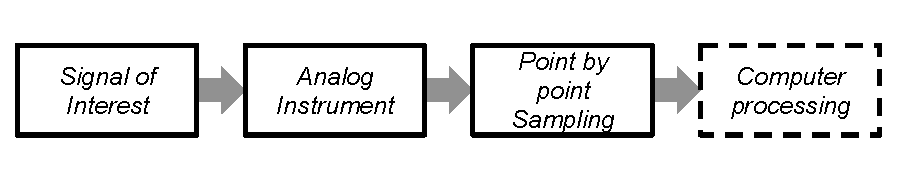
\includegraphics[scale=1]{isomorphicsensorflowchart}
    \caption{A systems view of a traditional sensing scheme. The signal-of-interest is incident upon the analog instrument. The analog instrument forms an isomorphism of the signal which is then periodically sampled point-by-point through an \gls{adc} device. Once the signal is in digital form, post-processing algorithms are often used to perform various tasks such as noise reduction, detection, and classification. Notice that the analog instrument, sampling scheme, and processing are all seperated. }
    \label{fig:isomorphicsesingflowchart}
\end{figure}


\begin{figure}
    \centering
    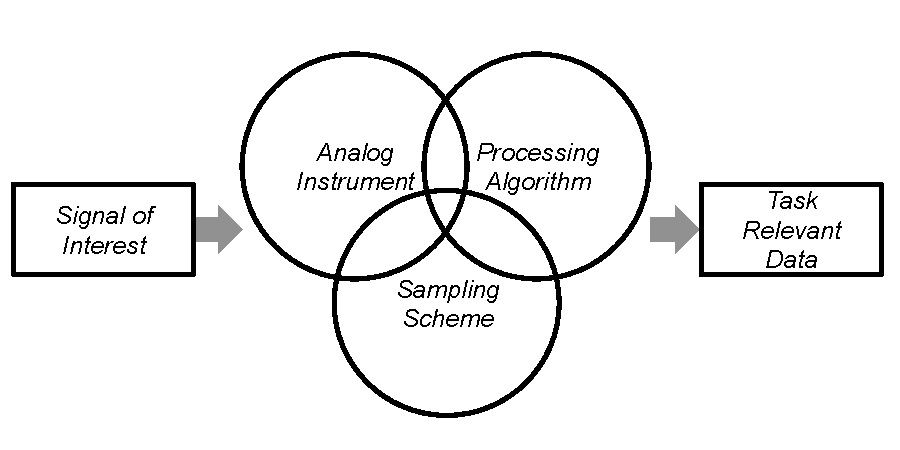
\includegraphics[scale=1]{computationalsensingflowchart}
    \caption{A systems view of a computational sensing scheme. The signal-of-interest is incident upon the analog instrument.  }
    \label{fig:computationalsensingflowchart}
\end{figure}


Rather than a rigorous discussion, this chapter will discuss some of the major developments and concepts in the field of computational sensing on an intuitive level. This will familiarize the reader with important terminology and techniques common in the field of computational sensing. A rigorous discussion with mathematical formalism of the concepts is given in \autoref{chap:Formalism}. This chapter will also discuss some of the challenges I and many other experimentalists and engineers have faced when developing computational sensing prototypes. I will close this chapter with a brief look ahead to the rest of the dissertation. 

%History%%%%%%%%%%%%%%%%%%%%

\section{Isomorphic Sensing}\label{sec:Isomorphic Sensing}

In Greek, the word isomorphic loosely translates to equal in form. Traditional sensors perform isomorphic sensing. In the context of this dissertation, an isomorphic sensor is any sensor which attempts to produce an output signal that resembles the signal-of-interest. In this paradigm, the analog instrument, sampling scheme, and post-processing algorithms are seperated.

We will discuss three important examples of isomorphic sensors: the pinhole camera, the photographic camera and the optical spectrometer (which I will just call a spectrometer from now on, even though there are many instruments called spectromers that not concerned with optical spectra). These sensors have had major roles throughout the history of optics and in the physical sciences so it is natural that they have also been the main focus of computational sensing. Therefore it is important we first understand the isomorphic version of these sensors.

In the photographic camera, the signal-of-interest is the object that is being photographed. This can be anything that is scattering or emitting light, a person, a tree or a distant group of stars. The analog instrument consists of the lens which is designed and fabricated to produce an image that is looks like the object at the \gls{fpa}. The more that the image resembles the object the better the optics. The \gls{fpa} then samples and quantizes the image and produces a digital representation of the object, measurement data. The measurement data is often is post-processed to perform such tasks as noise removal or to locate the object. 


There are two major sub-systems in the photographic camera which determine how well it performs: the optics and the FPA. Ideally, the optics (the analog instrument in this case) will produce a \gls{psf} which is infinitely small in diameter. For example, in a task such as the detection of a star from several neighboring stars in the night sky, if the \gls{psf} is much larger than the center to center seperation of the two stars in the optical image, it will be quite difficult to detect. A careful reader will note that this is the same argument used by Lord Raleigh in proposing his resolution criterion \cite{rayleigh1879investigations}. Even if the \gls{psf} is small enough, the \gls{fpa} must sample at a fine enough pixel-to-pixel spacing, called the \emph{pixel pitch}, to accurately reproduce the intensity variations at the scale which is pertinant to the task. Intuitively, this makes sense because if the image of both stars and the decreased intensity which signifies a certain amount of seperation between the two stars is imaged onto a single pixel, the one cannot ever hope to be able to accurately the detect the star without some other prior or side information. 

The pinhole camera predates the photographic camera over a thousand years, mostly due to it's simplicity. It consists of a small hole and a box which prevents any light except from the pinhole to enter, see Figure \ref{fig:pinholecamera}. The pinhole camera is useful for imaging in parts of the electromagnetic spectrum and particles for which there is no direct analog to refractive lens or reflective mirror. 

\begin{figure}
    \centering
    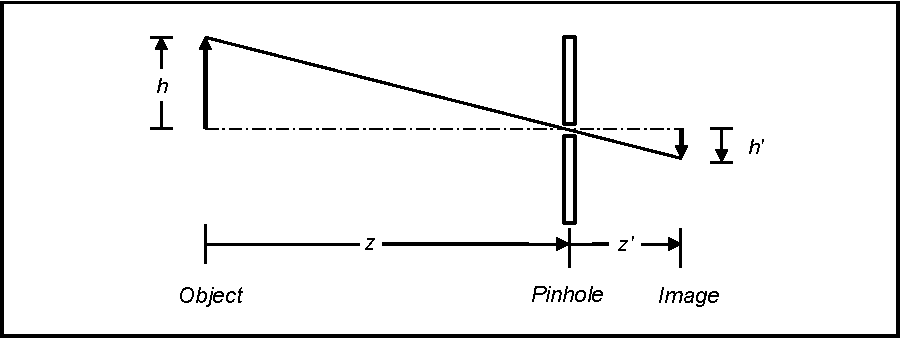
\includegraphics[scale=1]{pinholecamera}
    \caption{A pinhole camera.}
    \label{fig:pinholecamera}
\end{figure}

In the spectrometer, the signal of interest is the spectrum of the object. The optics are designed to take the incoming light and seperate various wavelength components, see Figure \ref{fig:slitspectrometer}. The part of the spectrometer which is used to physically isolate the wavelengths is called a \emph{spectrograph}. The result is a spectral intensity as a function of position at the \gls{fpa}. The \gls{fpa} and post-processing algorithms are used in the same manner as the photographic camera, which is to sample the optical spectrum creating digital version of it and to perform various tasks on the measurement data. For now, we will concentrate on the slit spectrometer, which measurements spectrum at a single point on the object.


\begin{figure}
    \centering
    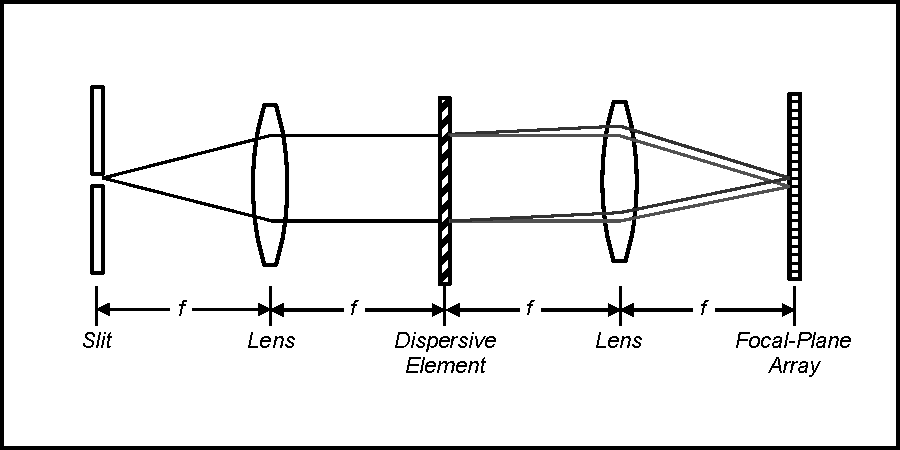
\includegraphics[scale=1]{slitspectrometer}
    \caption{An isomorphic slit spectrometer with a 4F configuration.}
    \label{fig:slitspectrometer}
\end{figure}

In the spectrometer, one of the important performance metrics is \emph{spectral resolution}, which we denote \gls{specres}. The spectral resolution is the smallest difference in wavelength the instrument can discern. Large spectral resolutions can degrade the spectrometers ability to discern important parts of the spectrum. Similarly with the camera, the \gls{fpa} must have a pixel pitch which is small enough in order to correctly sample the variations in the spectrum. 

The point-by-point nature of isomorphic sensing is both a strength and a source of weakness. 

The strength comes from the straightforward and intuitive architecture of the isomorphic sensor. Each subsystem: the optics, the \acrfull{fpa}, and the post-processing can be designed and constructed seperately as long as they meet their individual specifications. As long as the \gls{snr} is sufficient and the sampling rate is high enough we are guaranteed to recover the signal.

One of the weaknessess of the isomorphic approach however is the the ability to measure low \gls{snr} signals. Because the image is sampled in a completely parallel fashion at each exposure, each pixel contributes a certain amount of noise (which is independent of the signal strength). If the noise dominates, the measurement fidelity decreases often forcing the operator to incease the exposure time. For weak signals the exposure time can become prohibitive and for temporally dynamic signals this may lead to a loss of resolution. Indeed, one of the major engineering trade-offs faced by traditional spectrometer designers and users is that when one attempts to increase the light collection (increased slit-width) the spectral resolution \gls{specres} degrades (increases). Similarly, in the pinhole camera, there is a throughput versus spatial resolution trade-off, increasing the size of the pinhole degrades the \gls{psf}.


It would be easy to assume that with the recent revolution in machine learning and statistical signal processing combined with the dramatic increase in computing power that we could simply post-process poor measurments and obtain useful data. However, this isn't possible due to the an important theorem in information theory called the data processing inequality \cite{cover2012elements}. In layman's term it means "garbage in, garbage out".

Another weakness of isomorhic sensing is that the seperation of the analog instrument, the sampling scheme, and the data processing algorithms lead to increased \gls{swap-c}. As we mentioned in the photographic camera, the optics must be designed to produce a small \gls{psf}. For demanding applications, the optical design and fabrication can be the most expensive component of the sensor. While \gls{fpa} prices in the visible have fallen recently, \glspl{fpa} in certain parts of the electromagnetic spectrum can be quite expensive or non-existant \cite{noor2011compressive}.

In many cases, the signal is redundant and high resolution sampling becomes a waste of resources such as data storage and communications bandwidth. A good example is in photography where often the post-processing takes the digital image and applies a compression algorithm which looks for patterns in the signal and reduces the file size, discarding much of the sample data \cite{taubman2012jpeg2000}. 

The isomorphic sensor has served humanity well, however with all the weakness that have been discuss I will now begin to discuss some of major techniques in computational sensing that can be used to address some or all of the issues that I just stated. 

\section{Development of Multiplexing in Sensing}

\emph{Multiplexing} in sensing allows each measurement sample to be a combination of multiple points of the signal-of-interest. Multiplexing is a powerful tool that can be exploited by the sensor designer to eliminate or relax design trade-offs. 

A simple example which illustrates the usefulness of multiplex sensing is weighing objects. In this example, we are given a 100 sheets of paper. Let's assume that the scale's measurement error is insignificant. Isomorphic measurement sensing means one would need to measure each sheet of paper individually. Requiring 100 measurements. 

Now, let's say the scale's measurement error is on the order of the weight of the sheet. Measuring each sheet invidiually produces a large measurement error. In order to reduce the error to an acceptable \gls{snr} we need to make several measurements per sheet to reduce the error to an acceptable level.

However, we can be a little smarter. We can measure all 100 sheets at the same time. Since the weight of all 100 sheets is much larger than the measurement error of the scale, we can dramatically increase the precision of the measurement. If we can assume that each sheet is the same weight, then we are done. 

The weighing problem is analogous to the spectroscopy example. As discussed earlier in \autoref{sec:Isomorphic Sensing}, there is trade-off between light collection and spectral resolution. Increasing the slit-width to increase the amount of light has the effect of degrading the spectral resolution \gls{specres}. Around the late 1940's and early 1950's, several important papers and inventions demonstrated the effectiveness of multiplexing in spectroscopy. At the time the \gls{fpa} was non-existant, so in the slit spectrometer shown in \ref{fig:slitspectrometer}, where the \gls{fpa} is pictured, there was actually another slit. To record the intensity at each spectral channel, either the dispersive element or the exit slit had to be mechanically translated, making the measurements even slower by a factor of \gls{numspecchan}, the number of spectral channels of interest. 

Golay was the first to propose multiplexing the slit spectrometer by creating a pattern of binary (1's and 0's) entrance and exit slits \cite{golay1949multi}. The idea borrowed heavily from communications theory which is concerned with the reliable transmission of information over a noisey channel. In the Golay multi-slit spectrometer, the patterns of entrance and exit slits are matched based on mathematically useful properties, this is similar to coding and decoding signals in commucations. The entrance slits act to code the spectrum while the exit slits decoded the coded spectrum. Intuitively, the ability to use multiple entrance and exist slits increases the optical throughput of the spectrometer. Golay's idea dramatically increased the optical throughput without degrading the spectral resolution. 

Fellgett devised an alternative approach to multiplex spectroscopy, the Fourier Transform spectrometer, and was the first to note that multiplex measurements compared to isomorphic measurements improve the signal-to-noise ratio on the order of $ \sqrt{N_{\lambda}}$ \cite{fellgett1958principes}. He is generally credited with discovering the multiplex advantage, so it is often called the Fellgett advantage instead.

Another example that is pertinant to this dissertation is coded aperture imaging. Coded aperture imaging can be thought of as the multiplexed version of a pinhole camera. As mentioned earlier in \autoref{sec:Isomorphic Sensing}, there is a trade-off between the throughput and spatial resolution. However in many fields, such as high-energy particle imaging, refractive lenses and reflective mirrors are non-existant or underdeveloped. By using multiple pinholes the throughput is increased without sacraficing spatial resolution. However, the pattern of the pinholes, which is the code, in this case must be carefully designed to achieve optimal object reconstruction. Fenimore, Canon, and Gottesman were the first to create an elegant solution to coded aperture design called uniformly redundant arrays \cite{fenimore1978coded, gottesman1989new}.

In summary, multiplexing has the ability to eliminate classic trade-offs in isomoprhic sensors: signal strength or resolution. Modern researchers are still actively developing novel ways to implement multiplexing to increase resolution and senstivity in the spatial domain \cite{duarte2008single, townsend2012static}, spectral domain \cite{gehm2006static, tsai2013coded}, and temporal domain \cite{holloway2012flutter,llull2013coded}. However, multiplexing is not without its own set of problems. We now discuss inverse problems in computational sensing.

\section{Forward Models and Inverse Problems}

In the computational sensing community, a model which maps the signal-of-interest to the measurement data is called the \emph{forward model}. The problem of taking the observed data and calculating a reconstruction of the signal-of-interst or task-specific parameters is called the \emph{inverse problem}.

As you can imagine, solving inverse problems of isomorphic measurements, when one is concerned with reconstruction of the signal-of-interest, tend to be straight forward. In the weighing problem, the measurement is also the reconstruction. In the slit spectromer, where the forward model can be simply the continuous to discrete mapping of the spectrum. The spectrum is the interpolated measurement. 

Of course, we can begin to add various levels of complexity to the forward model to account for various physical aspects of the sensor, such as the fact the \gls{fpa} can't measure certain wavelength regions or the noise in our measurements. But again, assuming proper sampling and enough \gls{snr}, the reconstruction of the isomorphic signal is the measurement. This simplicity is one reason why isomorphic sensing still dominates at the consumer level despite all of the drawbacks I discussed earlier in \autoref{sec:Isomorphic Sensing}. 

However, the multiplexing of signal information forces us to develop computational steps to reconstruct or infer the parameters of the signal that caused the measurements. In the multiplexed weighing problem, a significant complication occurs when each sheet has a different weight. Now solving the inverse problem is not as straight forward. A single measurement of all 100 sheets in this case is an \emph{underdetermined problem} since we have 1 equation and 100 unknowns. What we can do is try measuring different combinations of the 100 sheets, each new combination provides us with a new equation to work with reducing the error. Niavely, we might assume that we can randomly choose 100 unique combinations and solve 100 equations using the algebra we were taught in high school. However when there is measurement error, in many applications including the weighing problem, random combinations are not the best way to conduct the coding, they are sub-optimal in terms of reconstruction error. This lead many to begin working on optimal coding strategies of signals for sensing and is major topic in this disseration.

In fact, the idea of multiplexing was not invented by Golay or Fenimore, what they contibuted was the creation of computationally simple ways to code and decode their signal-of-interest, making their sensors more appealling to a broader communicaty of scientists and engineers. A good example is the Hadamard matrix based code \cite{sloane1969codes}. The Hadamard code is appealling because reconstruction is simply the transpose of the original matrix. Unfortunately, not all multiplexing forward models codes have mathematically elegent inversion steps. Often the physics of the situation force non-isomorphic measurements which require a computational step to solve the inverse problem. 

\section{Indirect Imaging}

While Golay, Fennimore, and others were levering multiplexing to eliminate trade-offs in traditional sensors, an entirely disparate group of researchers were working on imaging techniques for which there was no isomorphic analog. In these cases the physics of the sensing modality prevents a point-by-point sampling of the signal-of-interest. These techniques are called indirect imaging. 

Perhaps one of the most successful early examples of indirect imaging and the rise of inverse problems in sensing is the development of radar. While early radar was concerned with the detection and distance of an object, development of imaging radar began after World War II. Imaging radar and specifically \gls{sar} can use time delay information combined with the doppler effects and interference patterns of coherent radio waves to create high resolutions of terrain and buildings. 

In medicine, an imaging modality that now common is X-Ray \gls{ct}, one is forced into this situation since the task is to reconstruct a 2 or 3-dimensional function from 1 or 2 dimensional measurement data. The forward model can be simple: In a collimated beam architecture with a 1-dimensional detector array, we say that each sample from each pixel on the array is proportional to the total number of x-ray photons that have not been aborped by the object \cite{radon20051} plus noise. The inversion of course is not straight forward. The culmination of the work related to the inversion techniques and the actual prototype resulted in the Nobel Prize for Physiology or Medicine in 1979 \cite{nobelprize1979medicine}. 

In general, non-isomorphic sensing such as indirect imaging schemes which include X-ray \gls{ct}, \gls{spect}, \gls{pet}, \gls{mri} and certain forms of sonic and radio wave imaging all require a data-processing or reconstruction step to solve an inverse problem \cite{barrett2013foundations}. In summary, the forward model of a sensor is essentially accounting for the physics which govern the measurement while the solving the inverse problem is a mathematical problem which attempts to either reconstruct the object or to calculate task-specific data of the object. 

We now turn to what are arguably the two most important inventions of optical sensing in the last several centuries, the digital image sensor and the digital computer. 

\section{The Digital Imaging Revolution}

Shannon, Nyquist, Wittaker and others established the theory for determining what the pixel spacing must be in order to properly sample the analog signal without loosing any information \cite{shannon1949communication, nyquist1924certain, nyquist1928certain}. 

\section{From Multiplexing to Compressive Sensing}\label{sec:multiplexingtocompressivesensing}

\section{Practical Considerations in Computational Sensing}

% Should this go in practical issues section?!?!
Decoding the signal, which we can also think of as solving the inverse problem is not necessarily straight forward. Unfortunately the coded of the analog signal and inversion steps are often seperately designed in computational sensing. This becomes especially frequency because the practicing sensor engineer must piece together various techniques from theorestist. This 

\section{Dissertation Overview}



%\bibliographystyle{IEEEtranS}  
%\bibliography{ThesisBib}


\chapter{Formalism}\label{chap:Formalism}

This chapter introduces the reader to the more rigorous concepts and mathematical background that will required to fully understand the material presented in the later chapters of this dissertation. 

A discussion of multiplexing and signal-to-noise ratio will be discussed, as well are various coding schemes used in various notable computational sensors as well as the ones in this disseration. 


The vast majority of modern optical sensing involves an \acrfull{adc} step, which creates discrete digital values from a physical phenomena. Therefore, we will concentrate on continuous-to-discrete and discrete-to-discrete measurements. This not only makes the formalism we will discuss more relavent but in many cases it will simplify the mathematics. 

As described earlier in \Cref{chap:Introduction}, a \gls{measurement} is a map from the physical signal-of-interest \gls{objvec} to the measurement data \gls{measvec}. The solutions to the electromagnetic wave equation are linear in free space so the propagation of electromagnetic radiation is linear. We can also approximately model the response of our sensors as linear. Thus we can write the measurement as an integral
%
\begin{equation}
	g_m = \int \mb{f}( \mb{x} ) h_m ( \mb{x} ) d \mb{x}
\end{equation}
%
where $ h_m ( \mb{x} ) $ is the continuous-to-discrete measurement process from point $ \mb{x} $ to discrete measurement index \gls{m}. We can write the continuous signal-of-interest as a superposition over a basis 
%
\begin{equation}
	f( \mb{x} ) = \sum_{n} f_n \psi_n ( \mb{x} )
\end{equation}
%
This allows us to express the measurement of any optical phenomena as a matrix multiplication
%
\begin{equation}
\mathbf{g} = \mathbf{Hf}
\label{eq:gHf}
\end{equation}
%
where \gls{measvec} is now a measurement data vector and \gls{objvec} is the discrete representation of the object signal-of-interest and $\mb{H}$ is the matrix which describes measurement process. For brevity we will refer to the \gls{objvec} as the object and $\mb{H}$ as either the sensing matrix or the measurement matrix. \Cref{eq:gHf} represents the forward model in a wide variety of computational sensors. The object \gls{objvec} is a vector in \gls{n} dimensional vector space and the measurement \gls{measvec} is a vector in \gls{m} dimensional vector space. In general $m \neq n$. Note that \Cref{eq:gHf} is an extremely useful way to represent the forward model in optics, since it allows us invoke a vast amount of computationally attractive numerical techniques which are dedicated to linear systems.

In the real-world noise degrades the measurements 
\begin{equation}
	\mb{g}=\mb{Hf} + \mb{e}	
\end{equation}
where \gls{noisevec} is additive noise. Additive noise is noise which is independent of the signal. An example of additive noise includes the thermal noise generated by the random fluctuations of the charge carriers from \gls{ccd} electronics. A different type of noise called multiplicative noise also exists, but will not be considered in this dissertation. 

\section{Isomorphic Sensing}

In an isomorphic measurement, where the goal is a one-to-one mapping of object points to measurement points, the measurement matrix is often modeled with the identity matrix
\begin{equation}
	\mb{H}=\mb{I}	
\end{equation}


We can get an idea of how much error exists in an isomorphic measurement through invoking the weighing example again. This example was originally discussed in book \cite{harwit2012hadamard} but it is so useful in the context of this dissertation I will briefly summarize it here. In the weighing example, let's say we have $4$ objects with true unknown weights $f_{1}, f_{2}, \cdots, f_{4}$. We record the measured weights $g_{1}, g_{2}, \cdots, g_{4}$ with additive noise (random error)  $ e_1, e_2, \cdots, e_4 $. The forward model with noise is 
\begin{equation}
	\left[ \begin{matrix} g_1\\ g_2\\ g_3\\ g_4\end{matrix} \right] = \left[ \begin{matrix} 1& 0& 0& 0\\ 0& 1& 0& 0\\ 0& 0& 1& 0\\ 0& 0& 0& 1\end{matrix} \right] \left[ \begin{matrix} f_1\\ f_2\\ f_3\\ f_4\end{matrix} \right] + \left[ \begin{matrix} e_1\\ e_2\\ e_3\\ e_4\end{matrix} \right] 
	\label{eq:gHfpluse}
\end{equation}
The estimated weights \gls{estobjvec} are the measurements  $ \mathbf{g} $
\begin{equation}
	\mathbf{ \hat{ f }} = \mathbf{g} 
\end{equation}
Where the error between the estimated weights and the actual weights is the error $ \mb{n} = \mbh{f} - \mb{f} $. For our purposes the assumption of a zero mean distributed noise is a good assumption. This allows us to assume the the isomorphic measurements are unbiased. For an unbiased estimator, the mean squared error of the estimated weight is the variance
\begin{equation}
	E [ ( \mb{e} )^2 ] = E [ ( \mbh{f} - \mb{f} )^2 ] = \sigma^2.
\end{equation}
The smallest possible mean square error is limited to the variance of the noise. Now, I will show how multiplexing codes can be used to reduce the mean square error of the estimate. 

\section{Multiplexing}

As we discussed in \cref{chap:Introduction}, \gls{multiplexing} is an extremely useful technique for overcoming trade-offs in traditional optical sensing. Now it is time to discuss and demonstrate the quantitative advantages provided by multiplexing. 

In a multiplexed measurement, each element in the measurement vector \gls{measvec} is a weighted linear combination of the elements in the object vector. Therefore the measurement matrix $\mb{H}$ is no longer an identity matrix. 



\subsection{Coding Schemes}\label{subsec:codingschemes}

We will now discuss formally the properties, advantages and disadvantages of several popular multiplex coding schemes used in computational sensing especially in dispersive spectroscopy such as the Hadamard, S-Matrices, and random coding. 

A Hadamard matrix of order $n$ is defined as a matrix \gls{hadamardn} as the $n \times n$ matrix whose elements consist of $+1$'s and $-1$'s and satisfies the following property:
\begin{equation}
	\mb{H}_{n}^T \mb{H}_{n} = \mb{H}_{n} \mb{H}_{n}^T = n I_{n}
\end{equation}
where $\mb{I}_n$ is an $n \times n$ indentity matrix. 

In multiplex spectroscopy and imaging, Hadamard codes are extremely popular for a variety of reasons. Hadamard codes are provably optimal in the case where we are allowed to take a full set of measurements, meaning that \gls{objvec} and \gls{measvec} from \cref{eq:gHf} are both vectors in $n$ dimensional space and when one uses both $+1$'s and $-1$'s in the code \cite{harwit2012hadamard}.  In this case, Hadamard codes achieves the minimal the mean square error defined as
\begin{equation}
	\text{MSE} = \frac{1}{n} ( e_1 + e_2 + \cdots e_n )^2 
\end{equation}

In the weighing example, we can get negative measurements by using a balancing scale instead of a spring scale. An Hadamard multiplexed measurement would look like
\begin{equation}
\left[ \begin{matrix} g_{1}\\ g_{2}\\ g_{3}\\ g_{4}\end{matrix} \right] =\left[ \begin{matrix} +1 +1 +1 +1 \\ +1 -1 +1 +1 \\ +1 -1 -1 +1 \\ +1 -1 -1 +1 \end{matrix} \right] \left[ \begin{matrix} f_{1}\\ f_{2}\\ f_{3}\\ f_{4}\end{matrix} \right]
\end{equation}
This means that in the first measurement all 4 items at placed in the same pan. In the second measurement items 1 and 3 are in the same pan while items 2 and 4 are in the opposite pan, etc \cite{harwit2012hadamard}. We have four equations and four unknowns so we can solve for the estimates using algebra

\begin{align*}
  \hat{f}_1 &= \frac{1}{4} (g_1 + g2 + g2 +g4) \\
  &= f_1 + \frac{1}{4}(e_1 + e2 + e3 + e4) \\
        \mathrel{\makebox[\widthof{=}]{\vdots}} \\
  \hat{f}_4 &= \frac{1}{4} (g_1 - g2 - g2 +g4) \\
  &= f_4 + \frac{1}{4}(e_1 - e2 - e3 + e4)
\end{align*}
The mean square error of the $m^{th}$ measurement  
\begin{equation}
	E [ ( \hat{f}_{m} - {f}_{m} )^2 ] = \frac{1}{4} \sigma^2.
\end{equation}
which is $4$ times lower than using an isomorphic measurement scheme. In general, the \gls{mse} of a Hadamard measurement is 
\begin{equation}
	\text{MSE} = \frac{\sigma^2}{N_{\lambda}}
	\label{eq:hadamardmse}
\end{equation}
where \gls{numspecchan} is the number of spectral channels, which is equal to the number of measurements \gls{nummeas}. Hotelling proved in 1944 that for a measurement matrix with elements $h_{mn} \in [-1, +1]$ the lowest possible MSE for the case of a full set of measurements is with a linear unbiased estimator is $\text{MSE} = \frac{\sigma^2}{N_m}$ \cite{brady2009optical}. So, one cannot possibly do better than Hadamard coding in this case. We will see later in other special cases that we can beat Hadamard codes.

In many practical cases in computational sensing, making a code with simultaneous positive and negative modulation of the signal is not possible. For incoherent light, the response is linear in intensity. In the case where one has the ability to make a full set of measurements but is limited to elements of $+1$'s and $0$'s, an S-Matrix code minimizes the \gls{mse} \cite{harwit2012hadamard}.

In the weighing example, a spring balance rather than a two pan scale analogous to this situations. 
\begin{equation}
\left[ \begin{matrix} g_{1}\\ g_{2}\\ g_{3}\\ g_{4}\end{matrix} \right] = 
\left[ \begin{matrix} 0 & +1 & +1 & +1 \\ +1 & +1 & 0 & 0 \\ +1 & 0 & +1 & 0 \\ +1 & 0 & 0 & +1 \end{matrix} \right]
\left[ \begin{matrix} f_{1}\\ f_{2}\\ f_{3}\\ f_{4}\end{matrix} \right]
\end{equation}
So items 2, 3, and 4 are weighed together, then 1 and 2, and so on. Solving the system of equations in a silimar fashion as before in the Hadamard weighing example we find that the mean square error for the $m^{th}$ measurement when weighing 4 items is 
\begin{equation}
\text{MSE} = E [ ( \hat{f}_{m} - {f}_{m} )^2 ] = \frac{7}{9} \sigma^2.
\end{equation}
Which reduced the \gls{mse} compared to the isomorophic measurement scheme but it is less of a reduction compared to the Hadamard measurement scheme. The \gls{mse} of the S-Matrix is approximately a factor of 4 increase compared to the Hadamard matrix coding scheme. 

In the case when the full set of measurements are availible, random coding schemes are provably sub-optimal to compared to Hadamard and S-Matrix codes. However, they should not be ignored because in compressive sensing, certain theoretical garuntees exist for random coding that do not exist for Hadamard and S-Matrix codes. Sometimes, the physics of the situation forces a random coding scheme. There is little literature on the performance of random coding schemes. At the time of this writing (2016), I am unaware of an optimality proofs for random codes when one has a full set of measurements availible. 

\subsection{The Fellgett Advantage}

The \gls{Fellgett advantage} is the improvement in \gls{snr} that occurs when an instrument takes multiplexed measurements compared to isomorphic measurements \cite{fellgett1958principes, davis2001fourier}. Physically the \gls{Fellgett advantage}  occurs because a single detector element produces a noise contribution whether it's sampling a single part of the object or multiple parts of the object. Maximizing the \acrfull{snr} of the estimated object signal-of-interest for a given system throughput and detector noise is major design consideration in computational optical sensing particularly in the area of spectroscopy. In spectroscopy, there are two well known multiplex schemes, the Hadamard multiplexing in dispersive spectrometers and the interferometric spectrometer . 

The \gls{fts} architecture is a similar to the Michelson interferometer, see Figure \ref{fig:fourierTransformSpec}.The \gls{fts} operates by taking the autocorrelation of the complex electric field as a function of time delay by moving one of the mirrors in the interferometer \cite{davis2001fourier}. The Wiener-Khinchin theorem says that for a wide-sense stationary random process, the Fourier transform of the autocorrelation is the power spectral density. Thus a computational post-processing step is required to reconstruct the spectrum from the measurement data. Since the \gls{fts} measures combinations of multiple wavelengths at each detector readout it also exhibits the \gls{Fellgett advantage}.

The advantage that multiplexing provides over an isomorphic measurement depends on the coding sceheme. We've just seen that for a Hadamard coding scheme the \gls{mse} is given by \Cref{eq:hadamardmse}. It turns out that for a \gls{fts} the \gls{mse} obtained is a factor of two greater than the Hadamard multiplexing scheme \cite{tai1976fourier}. 

\begin{equation}
	\text{MSE} = 2 \frac{\sigma^2}{N_{\lambda}} 
\end{equation}


\begin{figure}
	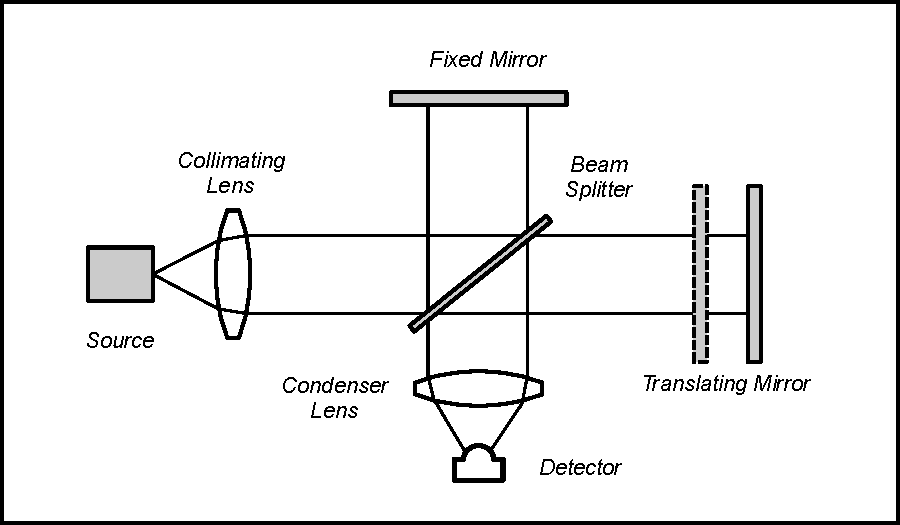
\includegraphics[scale=1]{fourierTransformSpec}
	\captionof{figure}[The architecture of the Fourier Transform Spectrometer.]{The architecture of the Fourier Transform Spectrometer resembles the Michelson interferometer. One of the mirrors is translated back and forth. The interferogram is the detected intensity versus mirror delay which is related to the autocorrelation of signal. The Fourier transform of the autocorrelation provides the spectrum.}
	\label{fig:fourierTransformSpec}
\end{figure}


\section{Principal Component Analysis}

Principal component analysis (PCA) is a technique that attempts to recast a dataset in manner which allows us to maximally discriminate the data with just a few vectors. The first vector points in the direction of maximum variance. The second vector points in a direction that also maximizes variance but is orthogonal to the first vector and so on. These new vectors are called the \emph{principal components}. We will say the \emph{rows} of matrix $\mb{P}$ are the principal components. 

Let's say we have a dataset $\mb{S}$ which consists of $N$ spectra with \gls{numspecchan} spectral channels. Instead of looking at the data as just intensity versus spectral channel, \gls{pca} attempts to construct a set of new vectors (also called features) that show as much variation in the spectra as possible. In other words, first direction (principal component) is used to recast the data to look as different (uncorrelated) as possible. This allows us to discriminate the data, as best we can with just one direction. The second principal component is the direction that provides the second most ability to discriminate the data, and so on. 

The covariance matrix is defined as
\begin{equation}
\mb{C_{X}} = \frac{1}{N} \mb{S} \mb{S}^{T}.
\end{equation}
Each element in the covariance matrix $C_{Xmn}$ is the covariance of the $m^{th}$ spectrum $\mb{s}_m$ and the $n^{th}$ spectrum $\mb{s}_n$. 
\begin{equation}
C_{Xmn} = \frac{1}{N} \mb{s}_m \mb{s}_n^{T}.
\end{equation}

Note that large covariance means they look quite alike and therefore are difficult to disambiguate.

If the entire collection of spectra $\mb{S}$ were mutually orthogonal, being able to tell one spectrum apart from another would be easy. You would just have a collection of spikes at different spectral channels. The covariance matrix in this case would be a diagonal matrix. 

Since there is typically some redundancy between spectra, the off-diagonal elements of the covariance matrix will be non-zero. The principal components allow us to recast the data to make it as uncorrelated as possible in a new basis. 
\begin{equation}
	\mb{Y} = \mb{PX}
\end{equation}
where $\mb{Y}$ is the data projected onto the principal component basis $\mb{P}$. The covariance of the projected data
\begin{equation}
	\mb{C_{Y}} = \frac{1}{N} \mb{Y} \mb{Y}^{T} 
\end{equation}
is a now diagonal matrix. Indeed, the principal components are the optimal way to discriminate the spectra in the dataset \cite{}.

It turns out there is a way to calculate the principal components in closed form. The \emph{eigenvectors of the covariance matrix are the principal components} \cite{shlens2014tutorial}. 

Since the full set of principal components forms a basis, each spectra $\mb{s}$ in $\mb{S}$ can be written as a superposition of principal components without any error
\begin{equation}
\mb{s} = \sum_{\lambda = 1}^{N_{\lambda}} y_{\lambda} \mb{v}_{\lambda}
\end{equation}
In many cases, only a few of the first principal components are needed in the summation to approximate the original data well.
\begin{equation}
{\mb{s}} \approx \sum_{\lambda = 1}^{M} y_{\lambda} \mb{v}_{\lambda}
\end{equation}
Where $M \ll N_{\lambda} $. Note that each eigenvector has an associated eigenvalue. The eigenvalues are also informative because they can tell us how many principal components are really needed to discriminate all of the spectra. The magnitude of the eigenvalue tells us how well it's associated eigenvector is at discriminating the data.

This is another reason why \gls{pca} is so useful. It can be used as a type of lossy compression code and as a measurement matrix for compressive sensing. Simply project the data onto the first several principal compoenents associated with the largest $M$ eigenvalues. 

The \gls{afssi-c} relies on a variation of Principal Component Analysis (PCA) for discriminating between spectra. In addition to \gls{pca} the AFSSI-C uses a Bayesian probability to create adaptive codes. We will now discuss some of fundamentals of Bayesian probability and the Log-likelihood ratios. 

\section{Bayesian statistics and Maximum a Posteriori}

In the real world, measurements are corrupted by noise. The random nature of noise corrupted measurements lends itself to a stochastic perspective of signals. A hypothesis can be associated with various parameters or aspects of a signal. A hypothesis is nothing more than a claim or premise that one is interested in verifying. In imaging and spectroscopy, one example is that at a certain location in the field of view, the hypothesis is that a spectrum is present or not present. Another hypothesis is that the mean value of the signal is some value. Instead of attempting to determine whether a hypothesis is true, often times we are interested in estimating parameters of stochastic processes, which we denote $\theta$.

Bayesian statistics allows one to treat the hypothesis or parameters as random variables rather than deterministric constants. A wide variety of Bayesian approaches exist and each require a heavy reliance on Bayes's theorem. Bayes' theorem is a way of computing probabilities of a hypothesis given some evidence which are related to the hypothesis. For example, Bayes' theorem can be used to decide which of two bags of candy has been opened or if a spectrum is present. The idea is that we can make a more informed calculation of probability if we are able to account or update the probability given some new piece of evidence that we may have not had at the beginning.

The derivation of Bayes' theorem follows from the definition of conditional probability, the conditional probability of event $A$ occuring given that $B$ occured is:

\begin{equation}
	P \left( A \given[\big] B \right) = \frac{ P \left( A \cap B \right) }{ P \left( B \right)}
\end{equation} 
this can be seen graphically in Figure


\begin{figure}
	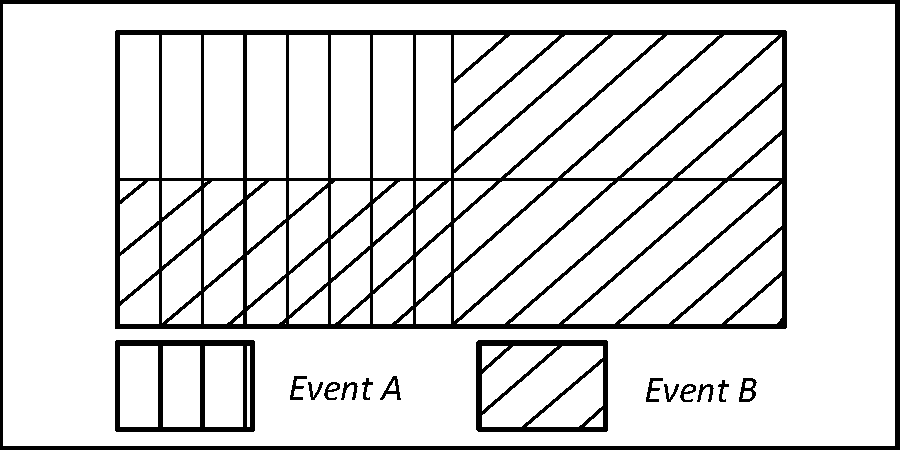
\includegraphics[scale=1]{definitionOfConditionalProbability}
	\captionof{figure}[Graphical demonstration of joint probability.]{Graphical demonstration of joint probability. The probability of event $A$ is $P(A)=3/4$. The probability of event $B$ is $P(B)=3/4$. The joint probability of events $A$ and $B$ is $P(A \cap B) = 1/4$. The probability of event $A$ occuring given that event $B$ has occured is $P( A \given B) = 1/3$. This is consistent with the equation $ P(A \cap B) = P(A \given B) P(B) $}
	\label{fig:definitionOfConditionalProbability}
\end{figure}

solving for the joint probability $ P \left( A \cap B \right) $ gives
\begin{equation}
 P \left( A \cap B \right) =	P \left( A \given[\big] B \right)  P \left( B \right)
\label{eq:bayeStep2}
\end{equation} 
since the joint probability commutes $ P \left( A \cap B \right) = P \left( B \cap A \right) $, we can also write
\begin{equation}
 P \left( A \cap B \right) =	P \left( B \given[\big] A \right)  P \left( A \right)
\label{eq:bayeStep3}
\end{equation} 
equatin the right hand side of Equation \ref{eq:bayeStep2} and Equation \ref{eq:bayeStep3} gives use Bayes' theorem (also called Bayes' rule)
\begin{equation}
	P \left( A \given[\big] B \right) = \frac{ P \left( A \right) P \left( B \given[\big] A \right) }{ P \left( B \right) }
\end{equation}

One interpretation of Bayes' theorem is called the Diachronic interpretation, which says that conditional probability of the hypothesis or parameter $\theta$ given knowledge of some evidence or measurement data $g$ is given by 

\begin{equation}
	P \left( \theta \given[\big] g \right) = \frac{ P \left( \theta \right) P \left( g \given[\big] \theta \right) }{ P \left( g \right) }
	\label{eq:diachronic}
\end{equation}

The term $ P \left( \theta \given[\big] g \right) $ is called the posterior. It represents our belief in the hypothesis given the data. The term $ P \left( \theta \right) $ is called the prior. $P \left( g \given[\big] \theta \right)$ is called the Likelihood. $P \left( \theta \right)$ is called the normalizing constant. In general the normalizing constant can be written as 
\begin{equation}
P \left( \theta \right) = \sum_{i} P \left( \theta_i \right) P \left( g_i \given[\big] \theta_i \right)
\label{eq:normalizingConstant}
\end{equation}
One can repeatly apply Bayes' theorem given new measurement data. We will use a simple example to illustrate how to update the belief. Imagine we have two bags of candy. Bag 1, which we denote $B_1$, has 10 pieces of cherry flavored candy, denoted as $C$, and has 30 pieces of strawberry flavored candy, denoted as $S$. Bag 2, $B_2$, has 20 pieces of cherry candy and 20 pieces of strawberry candy. At the beginning, the prior probability of selecting bag 1 or bag 2 is both equal
\begin{equation}
	P \left( B_1 \right) = P \left( B_2 \right) = \frac{1}{2}
\end{equation}
Someone then picks a bag at random and takes out a piece of candy that turns out to be strawberry flavor. What is the probability that bag 1 was selected? We can use Bayes' theorem to compute this

\begin{equation}
	P \left( B_1 \given[\big] S \right) = \frac{ P \left( B_1 \right) P \left( S \given[\big] B_1 \right) }{ P \left( S \right) }
\end{equation}

Where $ P \left( S \given[\big] B_1 \right) $ means the probability of selecting a strawberry candy assuming we have selected bag 1, which is $3/4$. The $ P \left( S \right) $ is the probability of selecting a strawberry candy from either bag 1 or bag 2, which $5/8$. Thus

\begin{equation}
	P \left( B_1 \given[\big] S \right) = \dfrac {\left( \dfrac {1} {2}\right) \left( \dfrac {3} {4}\right) } {\left( \dfrac {5} {8}\right) } = \frac{3}{5}
\end{equation}
Similarly, the probability that the person chosen bag 2 is $P \left( B_2 \given[\big] S \right) = 2/5$. Qualatatively, this makes sense, since bag 1 contained more strawberry flavored candy, the belief that bag 1 was chosen should increase and the belief that bag 2 was not chosen should decrease.

Now let's continue the example. Say we put the first piece of candy back in the bag and draw another piece of candy, which turns out to be cherry flavor. Now we must update the beliefs with this new piece of information. We can keep using Baye's theorem, but the trick is that the posterior from the last draw is now used as the prior for the current update.

\begin{equation}
	P \left( B_1 \given[\big] C \right) = \frac{ P \left( B_1 \given[\big] S \right) P \left( C \given[\big] B_1 \right) }{ P \left( C \right) }
\label{eq:updatedBayes1}
\end{equation}

\begin{equation}
	P \left( B_2 \given[\big] C \right) = \frac{ P \left( B_2 \given[\big] S \right) P \left( C \given[\big] B_2 \right) }{ P \left( C \right) }
\label{eq:updatedBayes2}
\end{equation}

The probability of drawing a cherry flavored candy assuming bag 1 was chosen is $ 1/4$ and the probability of drawing a cherry flavored candy assuming bag 2 was chosen is $1/2$. We now must use Equation \ref{eq:normalizingConstant} to compute the normalizing constant, otherwise the posterior probabilities will not sum to 1. In this case $ P(C) = 7/20 $. Plugging these numbers into Equations \ref{eq:updatedBayes1} and \ref{eq:updatedBayes2} gives the updated posterior probabilities

\begin{equation}
	P \left( B_1 \given[\big] C \right) = \frac{3}{7} \approx 0.43
\end{equation}

\begin{equation}
	P \left( B_2 \given[\big] C \right) = \frac{4}{7} \approx 0.57
\end{equation}

Intuitively, drawing a cherry flavored candy has reduced our belief that bag 1 was chosen since bag 1 consist of only $1/4$ cherry flavor candies while bag 2 consisted of $1/2$ cherry candy. 

Sometimes one is given a set of possible parameters that we are interested in estimating, $ \mb{\theta} $, given some measurement data $ g $. The method of \acrfull{map} says the parameters  $ \mb{\theta} $ which maximize the posterior probability are the most likely parameters. 

\begin{equation}
	\mb{\theta}_{map} = \argminA_{\mb{\theta}} \: p\left( \mb{\theta} \given[\big] g \right) 
	\label{eq:map}
\end{equation} 
Using Bayes' theorem we can rewrite Equation \ref{eq:map} as 
\begin{equation}
	\mb{\theta}_{map} = \argminA_{\mb{\theta}} \: \frac{ p\left( g  \given[\big] \mb{\theta} \right) p\left( \mb{\theta} \right) } { p\left(  g \right) }
\end{equation} 
Maximizing the posterior is now equal to maximizing the likelihood and prior. In certain cases, one needs to decide between two sets of parameters or hypotheses. One can do an analogous technique of comparing the posteriors by using a ratio

\begin{equation}
	\frac{ p( \theta_i | g ) }{ p( \theta_j | g ) } = \frac{ p(g|\theta_i) }{ p(g|\theta_j)} \frac{p(\theta_i)}{p(\theta_j)}
\end{equation}
If the ratio is larger than some threshold value then one choses parameter $\theta_i$ and if the ratio is less than the threshold then one choses $\theta_j$. Similar to the earlier example of updating the posterior based on new data, one can update the \gls{map} decision based on new data. Define the likelihood ratio of the $m^{th}$ measurement as 
\begin{equation}
	\Lambda_m = \frac{ p(g_m|\theta_i) }{ p(g_m|\theta_j)}
\end{equation}
After each new set of measurement data $g_{m}$ is collected, one can update the posterior ratios by multiplying the likelihood ratio from the old set of data with the likelihood ratio of the new set of data. The ratio which includes all the updates from measurement $m = 1$ to measurement $m = N_m$ is written as
\begin{equation}
	\frac{ p( \theta_i| \{ g \} _{N_m} ) }{ p( \theta_j | \{ g \} _{N_m} ) } = \displaystyle\prod_{m=1}^{N_m} \Lambda_m \frac{p(\theta_i)}{p(\theta_j)}
\end{equation}
where the notation $\{ g \} _{N_m}$ represents the set of all data from measurement $m$ to $N_m$.

Bayesian statistics is a useful way to update one's belief in a hypothesis or estimate a set of parameters. The Bayesian perspective is a different from the classical perspective. A classical approach to statistical estimation views parameters of interest as deterministic but unknown constants. The Bayesian approach assumes that $\theta$ is a random variable whose particular realization we must estimate.

As we've just seen through the Bayesian approach, the ability to take advantage of new measurement data and prior knowledge is a powerful concept. We will continue on this theme as we discuss \gls{compressive sensing} which relies heavily on the prior assumption of \gls{sparsity}.

\section{Compressive Sensing}

The fundamental approach of \gls{compressive sensing} is that rather than sampling at a high rate and then compressing the sampled data, one can dramatically reduce the number of samples by sampling the signal in a compressed form. I will now discuss some of the more formal concepts of compressive sensing and some techniques to compressively sampling signals. This allows one to build some intuition about compressive sensing. In order to understand why compressive sensing is so powerful we should first discuss the conventional sampling strategy.


\subsection{The Nyquist-Shannon Sampling Theorem}

One of the most important results concerning the \gls{sampling} of continuous signals is the Nyquist-Shannon sampling theorem (often referred to as the \emph{sampling theorem} for short). The sampling theorem says that exact reconstruction of a continuous \gls{bandlimited signal} $f(x)$ is possible if the sampling frequency $f_s$ is atleast twice the maximum frequency $ B $ of the signal \cite{shannon1949communication}. Assuming that a bandlimited signal $f(x)$ has been sampled according to the sampling theorem, then exact recovery from the discrete samples $f_n$ is guaranteed.

However, if the sampling frequency is less than twice the maximum bandwidth $f_s < 2B$, then aliasing may occur in the reconstruction. Aliasing is the effect that high frequencies in the original signal will represented as lower frequencies after reconstruction and information contained in the high frequencies will be potentially lost \cite{proakis1988introduction}. 

Before we continue, it's important to clarify a small but important distinction between the meaning of \gls{sampling} and the meaning of a \gls{measurement}. A measurement is any process that maps physical phenomena which contains a signal-of-interest into measurement data. The measurement data may or may not be discrete. Sampling has a more precise mathematical definition. It is the process of mapping a continuous signal into a sequence of discrete numbers which are called the samples. 

\subsection{Sparsity, Incoherence, and the Restricted Isometry Property}

At first glance, \gls{compressive sensing} seems to go against the Nyquist-Shannon sampling theorem, however the sampling theorem's guarantee of exact reconstruction of a continuous signal relies on the assumption of a bandlimited signal and uniform periodic sampling, which leads to isomorphic sampling. \Gls{compressive sensing} makes different assumptions:  \gls{sparsity} and \gls{incoherence}. Combined with non-linear optimization techniques, \gls{compressive sensing} allows one to take far less samples without significant loss of information. Before we discuss how to actually do compressive sensing and some of its drawbacks, it is important to have a formal discussion of these concepts.

Most continuous signals $f(x)$ can be writen as a discrete summation of orthonormal basis functions
\begin{equation}
	f(x) = \sum_{n=1}^{N} x_n \Psi_n(x),
	\label{eq:expansionEquation1}
\end{equation}
where $x_n$ is the coefficients. I will call the vector $\mb{x} = [ x_{1} \: x_{2} \: \dots \: x_{N} ]^T$ the representation vector of the signal and $\mb{\Psi}$ the representation basis. This allows us to rewrite the signal as a matrix multiplication
\begin{equation}
	\mb{f} = \mb{\Psi}\mb{x}.
\end{equation}

As we discussed in \Cref{chap:Introduction}, any vector $\mb{x}$ is \gls{sparse} when all but a few of its entries are zero. A vector is called $K$-sparse when it has at most $K$ non-zero entries. In real situations, signals with strictly sparse representation vectors are unlikely. Fortunately, it is possible to have approximately sparse representation vectors, which are called \gls{compressible}. In other words, the sorted magnitudes of the coefficients $|x_n|$ quickly decay. When a signal has an expansion in terms of a compressible representation vector, we can intuitively understand \Cref{eq:expansionEquation1}. Discarding smaller coefficients will not significantly degrade the information in the signal \cite{candes2008introduction}. \footnote{From now on, I will use the words \gls{sparse} and \gls{compressible} interchangeably.} 

The concept of \gls{sparsity} is important in compressive sensing. Sparsity determines how efficiently one can acquire the signals. All things being equal, if $K$ decreases, then the reconstruction error tends to decrease. Sparse representations of the signal are not the only important prequisite for high probability reconstruction.

The random sensing basis is useful because of it's mathematical convience however, we shall show heuristically that incorporating additional prior knowledge of the statistics of the signal can reduce reconstruction error in reconstruction but other computational sensing tasks such as spectral classification. However, the options for compressive sensing bases are still quite limited.

In practice, the signal is sampled in a different basis than the representation basis. For example, while many natural signals have a sparse or compressible representation in various wavelet bases or Fourier bases, sampling using the representation basis is not practical or desirable in many cases. Often a sensing basis \gls{H} is used to perform the sampling. In traditional Nyquist-Shannon sampling, the sensing basis is a collection of delta functions. In compressive sensing for example, the sensing basis is the binary random coded aperture mask in a compressive imaging system \cite{duarte2008single}. In an \gls{lcos} based compressive sensing spectrometer, the sensing basis is a finite set of spectral filters \cite{oiknine2016along, yuan2015compressive}. In short, the representation basis allows a signal to be represented as a sparse vector, while the sensing basis is composed of the functionals that one samples with.

The equation which combines these concepts to model a compressive measurement is

\begin{equation}
	\mb{g} = \mb{H} \mb{\Psi} \mb{x} = \mb{H} \mb{f}
	\label{eq:gHf2}
\end{equation}
where \gls{measvec} is a $N_m \times 1$ measurement vector, \gls{H} is a $N_m \times N$ measurement vector, and $\mb{x}$ is an $N \times 1$ vector. A forward model in compressive sensing obeys \Cref{eq:gHf2} when $N_m \ll N$. 

One important concept in \gls{compressive sensing} is coherence. The coherence between the sensing basis $\mb{H}$ and the representation basis $\mb{\Psi}$ is
\begin{equation}
	\mu \left( \mb{H}, \mb{\Psi} \right) = \sqrt{n} \max_{1 \leq k, 1 \leq n}  | \langle h_k, \psi_j \rangle | ,
	\label{eq:coherenceDef1}
\end{equation}
which defines coherence as a measure of the largest correlation between any two elements of $\mb{H}$ and $\mb{\Psi}$. There is an alternate definition of coherence which is concerned with only the sensing matrix $\mb{H}$ (the sensing matrix is also called the measurement matrix or the system matrix).

\begin{equation}
	\mu \left( \mb{H} \right) =  \max_{k \neq j } \frac{ | \langle h_k, h_j \rangle | } { \left\| h_k \right\|_2 \left\| h_j \right\|_2 }.
	\label{eq:coherenceDef2}
\end{equation}
In this definition, the coherence is the maximum correlation between columns of the system matrix. 

Ideally, one would like to use as less measurements $N_m$ as possible without degrading the reconstructed signal. In \gls{compressive sensing}, the amount of measurements needed is a function of the sparsity and the coherence. Given a coefficient sequence $\mb{a}$ that is $K$-sparse then one needs
\begin{equation}
N_m \geq C \cdot \mu^2 ( \mb{H} , \mb{\Psi} ) \cdot K \cdot \log n
\label{eq:minMeas1}
\end{equation}
for a high probability of reconstruction, where $C$ is just a constant and $n$ is the dimensionality of the original signal.

\Cref{eq:minMeas1} shows the importance of sparsity and coherence in compressive sensing. Lower coherence and sparsity allows one to use less measurements \cite{duarte2008single}. The more incoherent---lower correlation---the two bases are, the higher the probability of succesful reconstruction of compressive measurements. Random matrices have a high probability of being incoherent with any basis \cite{candes2008introduction}. Using the alternate definition of coherence from \Cref{eq:coherenceDef2} produces similar qualitative results \cite{tropp2006just}. 

The isometery constant $\delta_K$ of a matrix \gls{A} $=\mb{H}\mb{\Psi}$ is the smallest number such that 
\begin{equation}
	\left( 1 - \delta_K \right) \left\| \mb{x} \right\|_{\ell_2}^{2} \leq \left\| \mb{A} \mb{x} \right\|_{\ell_2}^{2} \leq \left( 1 + \delta_K \right) \left\| \mb{x} \right\|_{\ell_2}^{2} 
\label{eq:rip}
\end{equation}
for all $K$-sparse vectors $\mb{x}$. The matrix \gls{A} obeys the \emph{restricted isometry property} (RIP) of order $K$ if $\delta_K$ is not too close to one \cite{candes2008introduction}. If RIP is satisfied, the sensing matrix \gls{A} approximately preserves the Euclidean length of signals. The \gls{rip} is an important theorectical result which allows robust compressive sensing where signals are corrupted by noise. Sensing matrices which have random entries obey the \gls{rip} with high probability \cite{candes2008introduction, duarte2008single, foucart2013mathematical}. 

All of the concepts I have just discussed can be understood at an intuitive level. Sparsity is the idea that the information content of a signal is relatively small compared to the amount of data which originally described the signal. Coherence extends that concept of how invertable a matrix is, the more linearly independent the system of equations, the easier it is to invert the matrix. The restricted isometry property is basically saying that any matrix with a small isometry constant will keep the distance between signal vectors the same. Why is this important? Think of a geometric picture, imagine noise as a sphere of uncertainty around the signal vectors. When the noise is small, two signal vectors can be mapped to a small part of the measurement space and still fit in that space. When one extracts the signal from the measurements, one can tell them apart. As the noise increases one wants the distance between measured signal vectors to at least stay the same and certainly not dramatic decrease, otherwise it will be difficult to tell the signals apart. The \gls{rip} is basically a way of seeing if a measurement matrix will pack the signal vectors with the space distance between them. A small amount of noise will lead to a small amount of reconstruction error instead of a small amount of noise leading to a large reconstruction error. 

\subsection{Solving Inverse Problems For Compressive Sensing}


Now that I have discussed what compressive sensing is mathematically, it is time to address how to actually solve the problem of extracting $\mb{x}$ from
\begin{equation}
	\mb{g} = \mb{Ax} + \mb{e}
	\label{eq:gTan}
\end{equation}
where $\mb{g}$ is the measurement vector, $\mb{x}$ is the sparse represetation of the signal, $\mb{A}$ is the linear mapping from $\mb{x}$ to $\mb{g}$, $\mb{e}$ is the noise vector, and the number of measurements $N_m$ is much less than the dimensionality of the sparse representation vector $N$. 


The least squares estimator (LS) estimator attempts to solve this inverse problem by minimizing the objective function 
\begin{equation}
	\sum_{n=1}^{N} \left( \mb{g} - \mb{A}\mb{x} \right)^2 = \| \mb{g} - \mb{A}\mb{x} \|_{2}^{2}.
\end{equation}
which is the $\ell_2$ norm between the given data \gls{measvec} and the forward model for the data $\mb{A}\mb{x}$. Notice, there are no probabilistic assumptions about the measurement data. It turns out that a closed form version of the LS estimator exists as

\begin{equation}
	\mbh{x} = \left( \mb{A}^T \mb{A} \right)^{-1} \mb{A}^T \mb{g}.
\end{equation}
where $\mbh{x}$ is the estimated value of $\mb{x}$.

The derivation of the closed form of the least squares estimator is given in Appendix \ref{app:Derivation of the Least Squares Estimator}. Alternatively, if the vector $\mb{x}$ is very large, solving the inverse problem in closed form maybe too computationally intensive, one may use the gradient descent algorithm or other types of iterative optimization algorithms to solve the least squares problem. While the \gls{ls} estimator may provide a solution when $N_m \ll N$, these solutions tends to overfit the data in these situations and does not take advantage of the prior knowledge of sparsity in reduce the solution space. Therefore, the unconstrained \gls{ls} approach tends to be sub-optimal for the compressive sensing problem.

There are a vast number of algorithms that claim to be designed for compressive sensing. A full discussion of each algorithm, estimator, and optimization technique is simply not feasible. The ones used by the author and notable ones in the community will be briefly discussed now and in the relavent chapters. Since this dissertation is geared towards those who wish to construct experimental computational sensors, full rigour is omitted and only intuitive justification is given for each type of algorithm.

One can catagorize compressive sensing algorithms in three groups: optimization methods, greedy methods, and thresholding-based methods. 

Many of the algorithm for compressive sensing are optimization algorithms, specifically called \gls{basis pursuit} algorithms  \cite{foucart2013mathematical}. Optimization algorithms are problems which serve to minimize (or maximize) an objective function $F_0$.
\begin{equation}
	\mbh{x} = \argminA_{\mb{x \in \mathbb{R}^N }} \: F_0 \left( \mb{x} \right)
\end{equation}
which is called an unconstrained optimization problem. Similarly, solving the problem
\begin{equation}
	\mbh{x} = \argminA_{\mb{x \in \mathbb{R}^N }} \: F_0 \left( \mb{x} \right) \text{\; subject to \;} F_n \left( \mb{x} \right) \leq b_n \text{\; \;}\forall \text{\;} n
\end{equation}
is a constrained optimization problem. If $F_n \text{\;}\forall \text{\;} n$ are all convex then then problem is a convex optimization problem. If  $F_n \text{\;}\forall \text{\;}n$ are all linear functions, then it is called a linear program (program is synonomous with optimization) \cite{foucart2013mathematical}.

Given measurements \gls{measvec} and knowledge that $\mb{x}$ is sparse or compressible, solving an optimization problem of the form 
\begin{equation}
	\mbh{x} = \argminA_{\mb{x}} \: \| \mb{x} \|_{0} \text{\; subject to \;} \mb{A}\mb{x} = \mb{g}
	\label{eq:l0min}
\end{equation}
where $\| x \|_{0}$ is the $\ell_0$ norm, which is equal to the number of nonzero entries in vector $\mb{x}$.\footnote{The $\ell_0$ norm is not strictly a norm and is actually a quasi-norm.} \Cref{eq:l0min} return $\mbh{x}$ that resembles $\mb{x}$ as long as the measurement noise is small. This is referred to as $\ell_0$-minimization. The constraint ensures the solution agrees with the observed measurement data. In other words, one wants the sparsest solution possible that agrees with the measurement data. 


The $\ell_1$ minimization or \emph{basis pursuit} algorithm is 



Given that one has prior knowledge of the existance of a sparse solution, a more intuitive approach is to rewrite the inverse problem to ensure that sparsity is part of the solution. 


Unfortunately, $\ell_0$-minimization is nonconvex which means that iterative methods may not converge to a solution. This is an important feature for inverse problems. A convex problem has the property that any local minimum is also a global minimum. In fact, it has been shown that for a general matrix $\mb{A}$, $\ell_0$- minimization is intractable \cite{aggarwal2007data}. 

Fortunately, one can minimize the $\ell_1$ norm 
\begin{equation}
	\mbh{x} = \argminA_{\mb{x}} \: \| \mb{x} \|_{1} \text{\; subject to \;} \mb{A}\mb{x} = \mb{g}
	\label{eq:l1min}
\end{equation}
where $\| \mb{x} \|_1 = \sum_{n}^{N}|x_n|$, and get excellent reconstruction in the case where \Cref{eq:minMeas1} and the \Cref{eq:rip} (the \gls{rip}) are satisfied. Additionally, \gls{l1}-minimization is a convex problem which allows for fast and accurate reconstruction \cite{donoho2006compressed, candes2006robust, foucart2013mathematical}. A more practical version of \Cref{eq:l1min} is written as
\begin{equation}
	\mbh{x} = \argminA_{\mb{x}} \: \| \mb{Tx} = \mb{g} \|_{2}^{2} + \tau \| \mb{x} \|_1
	\label{eq:l1regls}
\end{equation}
where $\tau$ is a non-negative number. \gls{tau} is called the regularization parameter and serves to change the sparsity level of the solution and can be used to account for noise in the vector which increases the robustness of the optimization. In this form, the problem is called $\ell_1$ regularized least squares (LS). $\ell_1$ regularization also appears in the context of basis pursuit denoising \cite{chen2001atomic}. In statistics, $\ell_1$ regularization is used in the LASSO algorithm for feature selection, therefore one often refers to \Cref{eq:l1regls} as the LASSO problem \cite{tibshirani1996regression}. 












%\bibliographystyle{IEEEtranS}  
%\bibliography{ThesisBib}




\chapter{Static Computational Optical Undersampled Tracker}\label{chap:Scout}

\section{Motivation for the Static Computational Undersampled Tracker}

In large-area persistent surveillance, traditional \gls{isomorphic} sensing systems must acquire, process, store, and transmit large amounts of data to achieve high spatial and temporal resolution. These sensors are typically on airborne platforms or orbiting satellites which leads to a large \acrfull{swap-c}. However, if one is interested in estimating the location of moving objects (tracking) rather than reconstructing the entire object scene, the information content in the signal-of-interest is relatively low. One can significantly lower the \gls{swap-c} by using a task-specific approach. To address the challenges of traditional target tracking, several colleagues and I designed, built, and demonstrated such a device called the \acrfull{scout} \cite{townsend2012static, stenner2010static}. This chapter will provide details in to how we developed the \gls{scout}.

Most of the current experimental demonstrations of \gls{compressive imaging} try to reconstruct the entire object scene or spatial-temporal datacube. For example, the \gls{cacti} sensor uses a temporally varying psuedo-random coded aperture during a single \gls{fpa} exposure and attempts to reconstruct a spatial-temporal datacube \cite{llull2013coded}. In another experimental compressive imager, a rotating cylindrical lens measures scene data using an optical Radon transform and then reconstructs a static object scene \cite{evladov2012progressive}. While these architectures demonstrate the rapid progress that researchers have made towards compressive imaging, they emphasize reconstructing high dimensional data and require another post-processing step to extract task-specific information. Furthermore, this data will then need to be compressed again for storage or transmission. If one is concerned with only tasks, then reconstructing the entire scene as an intermediate step is unnecessary and even wasteful. 

Another example of \gls{compressive imaging} is the single pixel camera, discussed in \Cref{sec:multiplexingtocompressivesensing}. This sensor uses a \acrfull{dmd} to measure in any arbitrary basis, but must do so over many time-sequential measurements \cite{duarte2008single}. Each measurement is an integrated point-by-point multiplication of the scene locations with the \gls{dmd} array values. For temporally static scenes, this architecture allows an arbitrarily long exposure time (within the limit of detector saturation) to increase the \gls{snr} for each measurement. However, with temporally varying scenes it needs to record all the projections for each frame before the object moves.  Increasing the rate at which projections are made is possible, but this reduces exposure time and \gls{snr}. One way to overcome this is by implementing a parallel architecture of single pixel cameras, each with a different projection, see \Cref{fig:parallelcsimager2}. Clearly this will significantly increase the \gls{swap-c} of the architecture. Another issue with a fully parallel architecture, is that each camera will have a different entrance pupil location, producing parallax. One issue many computational sensor designs must deal with is ``over multiplexing''. All real optical \gls{adc} devices have a certain amount of dynamic range, in which linearity is valid. As the amount of light that is recorded increases, the amount of dynamic range being used fills up. Architectures which only use a single pixel are at greater risk for over multiplexing. 

\begin{figure}
	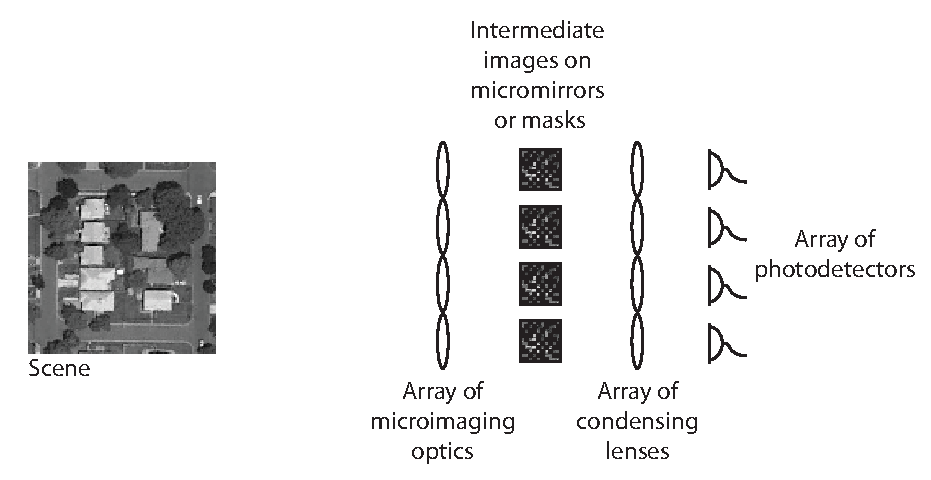
\includegraphics[scale=0.9]{parallelcsimager2}
	\captionof{figure}[The architecture of a hypothetical parallel single pixel camera to capture simultaneous projections.]{An example of a typical parallel optical CS architecture. Capturing $N_m$ simultaneous projections requires using $N_m$ spatial light modulators or masks and $N_m$ detector elements.}
	\label{fig:parallelcsimager2}
\end{figure}

A computational sensing architecture dedicated to target tracking rather than full object scene reconstruction, can significantly ameliorate these design trade-offs. We developed the \acrfull{scout} with the goal that measurements must be acquired ``single-shot'' using a conventional \gls{fpa} \cite{townsend2012static, poon2012advances}. The \gls{scout} system is an important step toward practical low-cost computational sensing for optical imaging. The system enables parallel ``single-shot'' acquisition of compressed, task-specific sensing oriented data, using a static (no moving parts) architecture. 

\begin{figure}
	\centering
	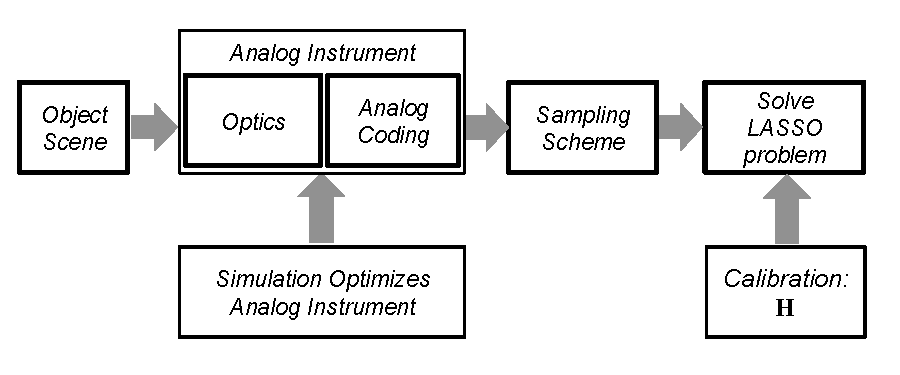
\includegraphics[scale=1.0]{scoutFlowchart}
	\captionof{figure}[Flowchart of \gls{scout} system architecture.]{A systems level flowchart of the \gls{scout} system. Light from the object scene propagates to the optical instrument which consists of a coded aperture (mask 1), an objective lens, and another coded aperture (mask 2), a \acrfull{fpa} then undersamples the coded object scene, measurement data is used to solve a \gls{lasso} problem. The parameters of the optical instrument is optimized using simulations to minimize the probability of tracking error. Calibration provides accurate measurement of the system matrix $\mb{H}$ to lasso optimization algorithm.}
	\label{fig:scoutFlowChart}
\end{figure}

A related static approach uses optical Radon projections \cite{kashter2012optical}. This instrument relies on a several cylindrical lenses to integrate the optical intensity from the object plane onto lines on the \gls{fpa}. The number of detector elements is much less than the native dimensionality of the object scene. For a single moving point in the field-of-view, two perpendicular Radon projections is enough to compute the change from frame to frame. However, the researchers found heuristically that four cylindrical lens are better for reconstructing the change information for an scene that included up to ten moving objects, called movers. 

A systems level flowchart of the \gls{scout} is shown in \Cref{fig:scoutFlowChart}. Like many computational sensors, it relies on the coding of the analog signal-of-interest prior to the \gls{adc} step and processes the measurement data using prior information and calibration data. The analog instrument was optimized using a custom ray-based simulation which evaluates a metric based on the simulated system matrix. In this chapter, I will discuss the \gls{scout} architecture in detail in \Cref{sec:ScoutArchitecture}, which uses a defocused imaging system with two binary amplitude masks. The \gls{fpa} samples at a much lower resolution than the native resolution of the object scene. While other compressive imaging systems have to reconstruct entire images, the \gls{scout} only reconstructs frame-to-frame differences. As a result the \gls{scout} requires significantly less bandwidth to transmit to a base station where the post-processing step can occur.


\section{SCOUT Architecture}\label{sec:ScoutArchitecture}

The goal of the \gls{scout} was to demonstrate a low \gls{swap-c} compressive target tracking sensor. The \gls{scout} architecture is designed to avoid the hardware scaling issues of the single-pixel camera. The trade-off for the ability to measure parallel projections is the loss of flexibility to implement arbitrary projections i.e. by using a \gls{slm}. However, rather than fully designing the projections themselves, I describe a process for optimizing the optical instrument  in \Cref{sec:ScoutSimulations}. Previous prototypes of the \gls{scout} architecture are described in \cite{stenner2010static, rivenson2010single}. 

The \gls{scout} system takes measurements that are both compressive and multiplexed: The number of measurements is less than the number of scene locations $N_m \ll N$, and each measurement must contain information about many scene locations. In this architecture, the number of measurements is the number of pixels in the \gls{fpa}. Intuitively this means that the system matrix must exhibit a many-to-few mapping from scene locations to \gls{fpa} elements. 


The \gls{scout} architecture is shown in \Cref{fig:scoutArchitecture}. In this architecture the \gls{multiplexing} occurs in the spatial domain by mapping multiple object scene locations to only a few detector pixels. To accomplish this, we created a structured blur. This blur allows the light from a single object point to be spread to several pixels on the \gls{fpa}. The most straightforward way to achieve a blur is by defocusing the image so that the \gls{psf} is broad, spanning many \gls{fpa} pixels. Since the number of \gls{fpa} pixels are less than the object scene resolution, the measurement is compressive. 


Like any aberration, defocus significantly reduces contrast of high spatial frequencies, so the measurements will be poorly conditioned for reconstruction. Therefore, we created high-frequency structure in the \gls{psf} by using two pseudo-random binary occlusion masks. Each mask is placed at different positions between the lens and the sensor. The separation between masks results in a spatially varying point-spread function. 




\begin{figure}
	\includegraphics[scale=1.2]{scoutArchitecture}
	\captionof{figure}[The SCOUT architecture.]{A diagram of the \gls{scout} architecture. A lens projects light through a pair of binary occlusion masks onto a low-resolution sensor which is defocused from the nominal image plane. This creates a spatially multiplexed shift-variant PSF incident on the \gls{fpa}.  }
	\label{fig:scoutArchitecture}
\end{figure}



As with many linear computational sensing architectures, the forward model is written in the form
%
\begin{equation}
	\mb{g} = \mb{H} \mb{f} + \mb{e}
\end{equation}
%
where $\mb{f}$ is the discrete representation of the object signal-of-interest, $\mb{g}$ is the measurement, $\mb{H}$ is the matrix which describes mapping of the object to the measurement, and $\mb{e}$ is the noise at each measurement. In this situation the signal-of-interest is actually the difference between two subsequent object scenes (frames) $\Delta \mb{f}$:
%
%
\begin{equation} 
\begin{split}
	\mb{g}_{k} &= \mb{H} \mb{f}_{k} + \mb{e}_{k} \\
	\mb{g}_{k+1} &= \mb{H} \mb{f}_{k+1} + \mb{e}_{k+1}
\end{split}
\end{equation}
%
Where the subscripts represent the $k^{th}$ readout from the \gls{fpa}.
%
\begin{equation}
	\Delta \mb{g} = \mb{g}_{k+1} - \mb{g}_{k} = \mb{H} \ap{ \mb{f}_{k+1} - \mb{f}_{k} } + \mb{e}_{k+1} - \mb{e}_{k} 
\end{equation}
%
%
so the forward model can be written as
%
\begin{equation}
	\Delta \mb{g} = \mb{H} \Delta \mb{f}  + \Delta \mb{e}
	\label{eq:scoutgHf}
\end{equation}
%
In this equation, the 2-dimensional difference frame and object scene have a resolution of $ R_x \times R_y$ elements, and are lexicographically reordered into a $N \times 1$ column vector, $\Delta \mb{f}$ and $\mb{f}$. Similarly, the difference measurement and measurement $\Delta \mb{g}$ and $\mb{g}$ are $N_m \times 1$ vectors representing a 2-dimensional \gls{fpa} readout with a $ r_x \times r_y$ matrix which represents the low resolution measurement. The detector noise is represented by the $ N_m \times 1 $ vector $\mb{e}$. The system matrix $\mb{H}$ is thus an $N_m \times N $ matrix, where $N_m \ll N$ in order to the system to be considered compressive. The $n^{th}$ column of the matrix is the \gls{psf} of the $n^{th}$ location in the object scene. The resulting system matrix $\mb{H}$ demonstrates that the \gls{scout} is a spatially variant optical system and presents a block structure, as seen in the example shown in \Cref{fig:scoutSysResponse}.

\begin{sidewaysfigure}
	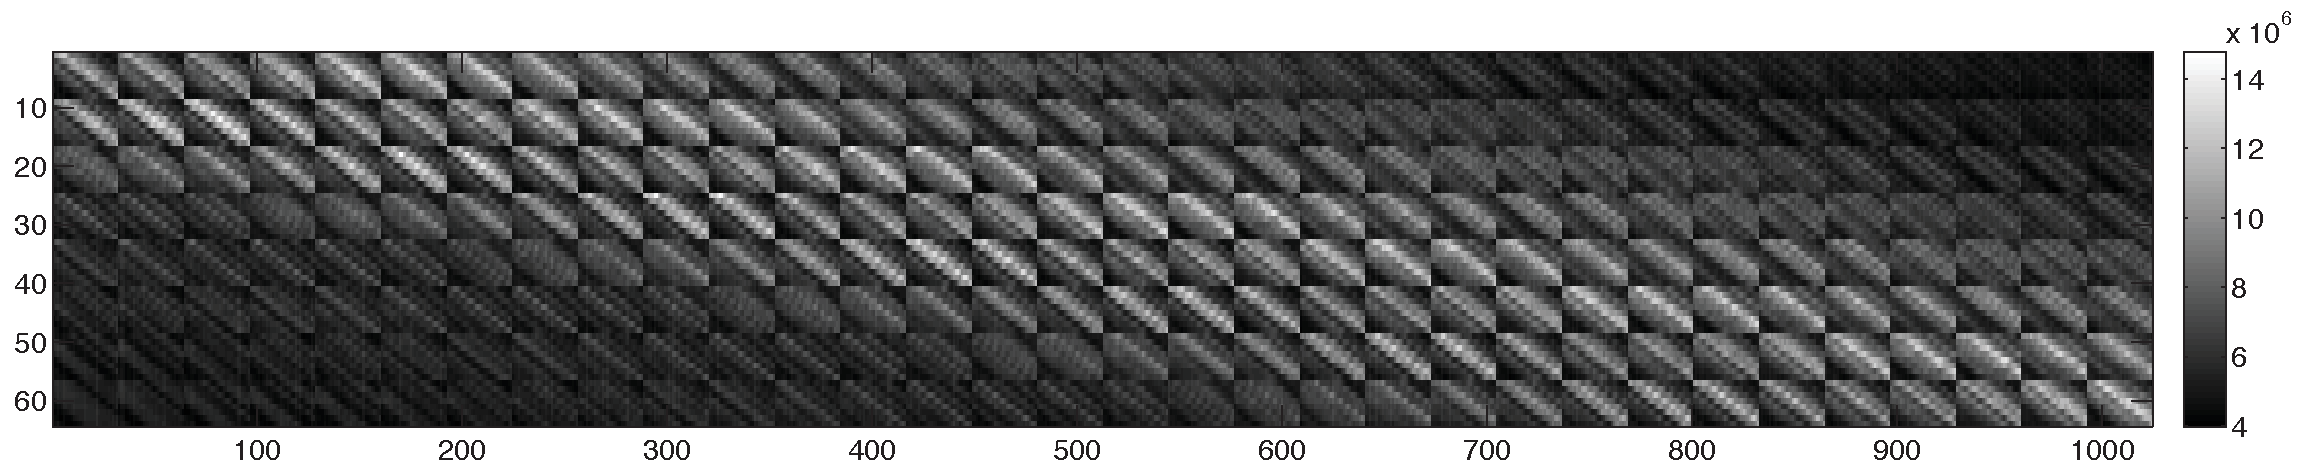
\includegraphics[scale=0.65]{scoutSysResponse}
	\captionof{figure}[An example of the system matrix of the \gls{scout}.]{An example of an experimentally measured of the system matrix of the \gls{scout} system. The approximate block-Toeplitz structure is clearly evident, as is the deviation from the Bernoulli or Gaussian ensembles typically considered in CS treatments. }
	\label{fig:scoutSysResponse}
\end{sidewaysfigure}


Referring back to the diagram of the \gls{scout} architecture shown in \Cref{fig:scoutArchitecture}. The object distance is much larger than the focal length of the lens so image of the scene occurs approximately one focal length from the lens $f_E$. The \gls{fpa} is placed some distance $d_{im}$ from the focal plane thus the total distance from the lens to the \gls{fpa} is $f_E + d_{im}$. Two binary occlusion masks, mask 1 and mask 2, are placed at distances $d_1$ and $d_2$ from the sensor. Mask 1 and 2 have associated fill factors $F_1$ and $F_2$ and pitch $p_1$ and $p_2$, respectively. 


\section{Optimizing the SCOUT}\label{sec:ScoutSimulations}

While the \gls{scout} lacks the ability to implement arbitrary measurement codes, we are able to adjust various physical parameters of the system such as defocus distance and mask fill factor to minimize reconstruction error. Adjusting each parameter in the actual prototype requires too much time, a more practical approach is to simulate the \gls{scout} architecture. In this section, I will discuss the simulation and define a metric that we used to evaluate different design parameters of the \gls{scout} without the need to reconstruct the difference frames. 

\subsection{Simulating a SCOUT System}

We developed a paraxial ray based simulation for the \gls{scout}. The simulation allows us to model the effects on the measurement as light travels through the lens and two masks and onto the detector plane. The lens is modeled as a single thin lens with transmittance function $t_f$ and the two masks have transmittance functions $t_1$ and $t_2$. From calibration measurements, the mask has a transmittances of $0$ where the mask is black and $0.88$ where the mask is clear. The lateral magnification of the scene and the two masks is calculated using similar triangles.

A simulated calibration occurs, in other words the simulation records the $r_x \times r_y$ PSF from each scene location in order to obtain the system matrix $\mb{H}$. Once $\mb{H}$ is known, we use it to simulate the low resolution measurements, $\mb{g}$, of the higher resolution scenes, $\mb{f}$. Subsequent simulated measurements are subtracted to find $\Delta \mb{g}$. We also did not add any noise. I have attached the simulation code in Appendix \ref{app:scoutSimCode}.


\subsection{Quantifying Reconstruction Error}

The \gls{mse} error metric is not suitable for our application because it weights all errors equally. For the task of motion tracking we classify errors into three types. A false positive occurs when the estimate shows an object where there is none. A false negative occurs when the estimate fails to show an object where one exists. As shift error occurs when an object is being tracked but appears in the wrong location. We developed a custom tracking error metric that weighs false negatives and false positives more than shift errors. This is because false negatives and false positives indicate a serious failure in the motion tracking task, while shift errors are less serious. We define tracking error as

\begin{equation}
	P = \frac{ | \mb{a}   \otimes \mb{\epsilon} |}{2N_{mv}}
	\label{eq:scoutErrorMetric}
\end{equation}
%
where
%
\begin{equation}
	\mb{a} = 
	\begin{bmatrix}
	    1/9 & 1/9 & 1/9 \\
	    1/9 & 1/9 & 1/9 \\
	    1/9 & 1/9 & 1/9 
	\end{bmatrix}
\end{equation}
%
where the error $\mb{\epsilon}$ is the difference between the true and reconstructed difference frames
%

\begin{equation}
	\mb{\epsilon} = \Delta \mb{f} - \Delta \mbh{f}
\end{equation}
%
and $N_{\text{mv}}$ is the number of movers in the scene. To reduce the penalty for one-pixel shift errors, the error frame is convolved with a three pixel averaging kernel $\mb{a}$. The absolute value is taken in order to count positive and negative errors equally, and the error is divided by $2N_{mv}$ to make the metric independent of the number of movers. 

\subsection{Optimizing Optical System Parameters}

Now that I have explained the simulation and the custom error metric for tracking, I can finally begin to discuss how we optimized some of the parameters to reduce the reconstruction error. Both the simulation and experimental study demonstrates a relationship between mask position and pitch: the tracking error is very sensitive to the \emph{projected} mask pitch on the \gls{fpa}. Furthermore, increasing the mask seperation reduced tracking error, generating a highly space-variant \gls{psf}. With these observations in mind, we focus our study on the mask pitches ($p_1$, $p_2$) as well as the defocus distance $d_{im}$. 

A brute force search, using the \gls{lasso} solver at each step is computationally intensive. We wanted a simple to compute metric which can predict tracking error. So we developed a custom metric inspired by the coherence parameter from the compressive sensing community, see \Cref{eq:coherenceDef1}. We created a customized coherence parameter $\mu$, 
%
\begin{equation}\label{defofcoherence}
    \mu = \max{\left| \langle h_i, h_j \rangle \right|} ;  \qquad i \neq j
\end{equation}
%
which is the maximum absolute value of the inner product between unique columns $h_i$ and $h_j$ of $\mb{H}$. The columns are unnormalized because their relative magnitude is related to the physical light throughput. 

Notice that although system matrices with nearly pairwise orthogonal columns will result in small coherence values, system matrices with numerically small entries can accomplish the same. Optimizing $\mb{H}$ for minimum coherence would drive total system throughput down. To eliminate this effect we normalized $\mb{H}$:

\begin{equation}
	\mb{H}_{norm} = \frac{ \mb{H} }{ \sum_{m = 1}^{N_m} \sum_{n = 1}^{N} h_{m,n} }
\end{equation}
%
where $N_m$ and $N$ are the total number of rows and columns in the system matrix. Physically, this normalization represents division by the sum of each PSF’s light throughput. The coherence of a system matrix normalized in this way cannot be biased by reducing throughput. One consequence of this normalization is that mask fill factor cannot be optimized.

\begin{figure}[!ht]
	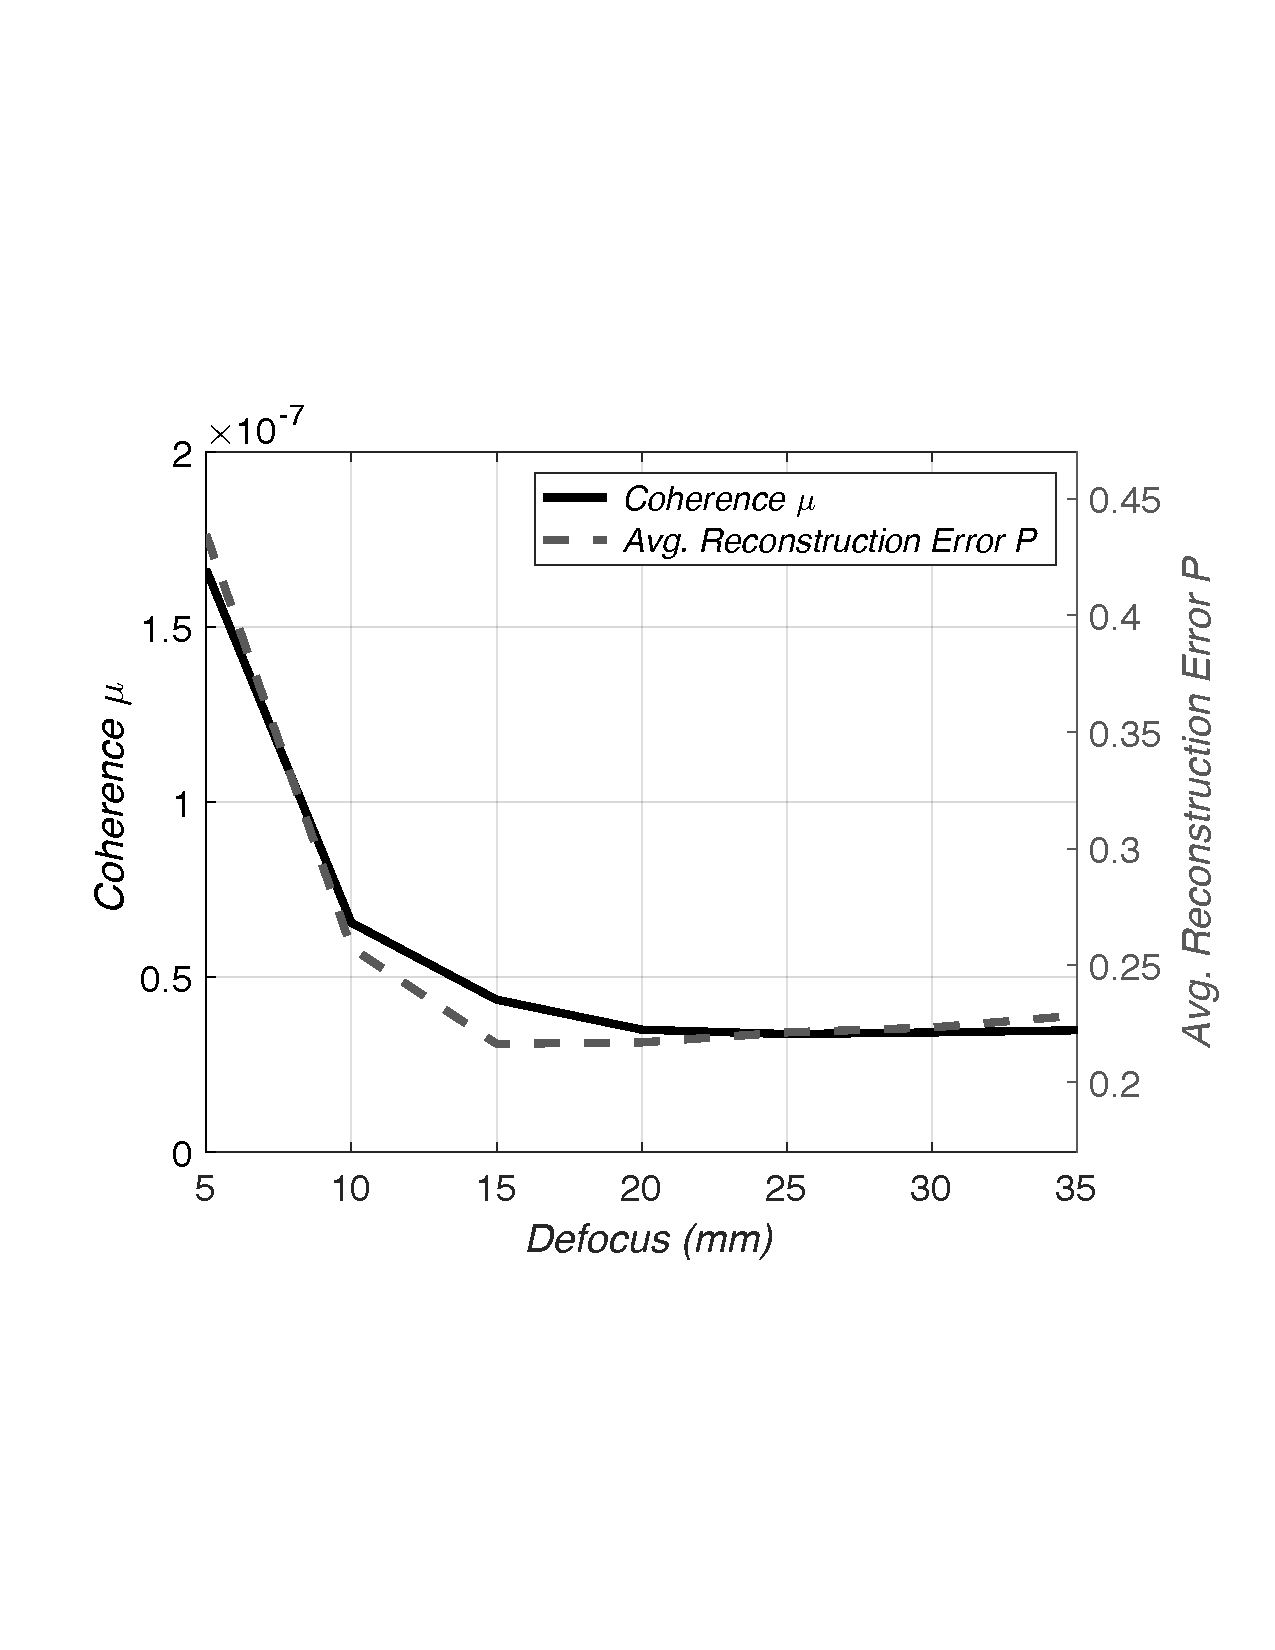
\includegraphics[scale=0.75]{coherenceAndReconErrorVsDefocus}
	\captionof{figure}[The coherence and reconstruction error versus defocus distance.]{The coherence $\mu$ (left vertical axis - black) and reconstruction error P (right vertical axis - dashed gray) plotted as a function of defocus distance $d_im$. }
	\label{fig:coherenceAndReconErrorVsDefocus}
\end{figure}

\begin{figure}[!ht]
	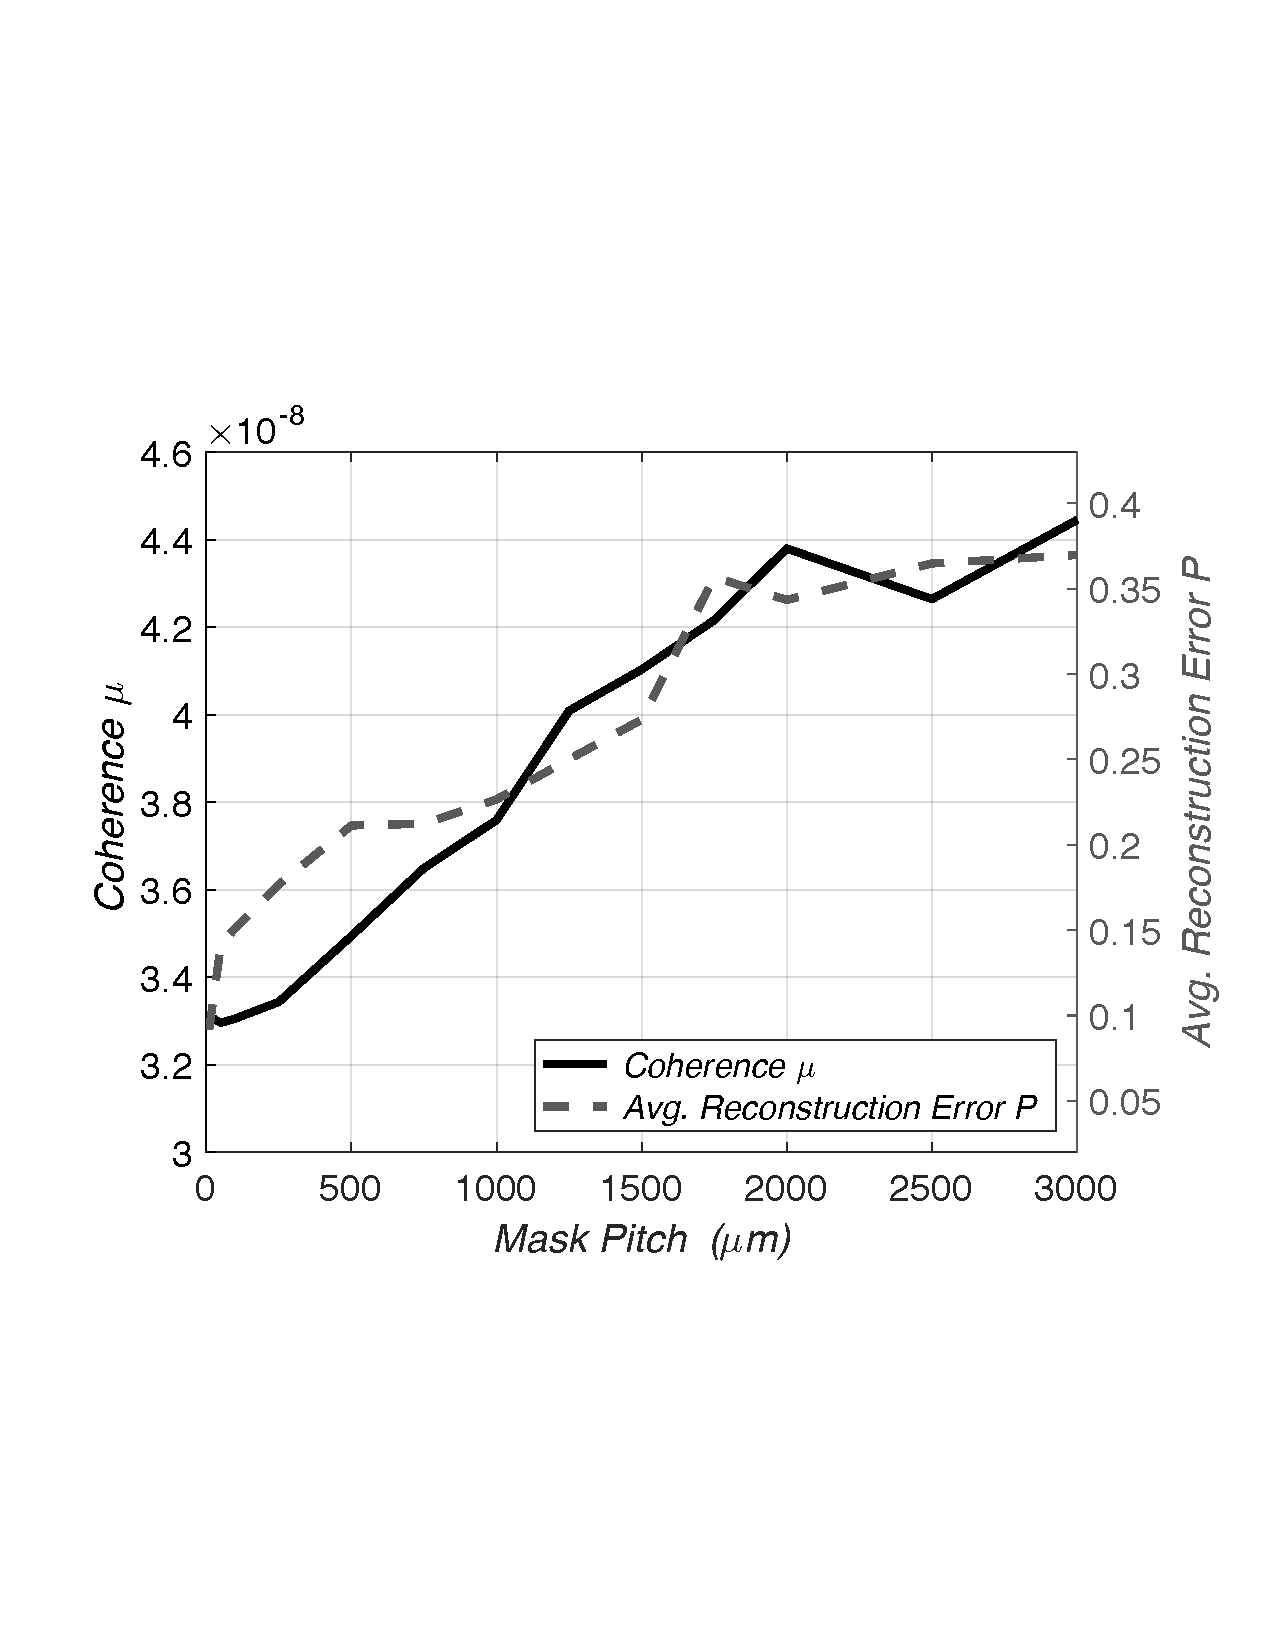
\includegraphics[scale=0.75]{coherenceAndReconErrorVsMaskPitch}
	\captionof{figure}[The coherence and reconstruction error versus pitch of mask 2.]{The coherence $\mu$ (left vertical axis - black) and the reconstruction error P (right vertical axis - dashed gray) is plotted as a function of the pitch of mask 2 }
	\label{fig:coherenceAndReconErrorVsMaskPitch}
\end{figure}


\begin{figure}[!ht]
	\centering
	\includegraphics[scale=0.65]{scoutExpSetup1}
	\captionof{figure}[Photograph of \gls{scout} recording a moving object scene of a black background.]{The camera captures images of scenes displayed on a plasma television approximately 2 meters away..}
	\label{fig:scoutExpSetup1}
\end{figure}

\begin{figure}[!ht]
	\centering
	\includegraphics[scale=0.85]{scoutExpSetup3}
	\captionof{figure}[Photograph of \gls{scout} camera disassembled to show the lens and the first mask.]{The camera disassembled to show the camera body, the optical tube and the custom fabricated lens holder which goes inside the lens tube.}
	\label{fig:scoutExpSetup3}
\end{figure}

To demonstrate the effectiveness of the modified coherence parameter as a predictor of reconstruction error trends, I ran several simulations with complete reconstructions in order to compare reconstruction error to coherence. \Cref{fig:coherenceAndReconErrorVsDefocus} shows that reconstruction error and the coherence parameter follow similar trends for different defocus distances when all other parameters are held constant. \Cref{fig:coherenceAndReconErrorVsMaskPitch} shows similar agreement when varying values of mask pitch $p_2$.

The simulations demonstrate the viability of the architecture and provide an efficient way to optimize most architecture parameter values using the simulated system matrix coherence. Mask throughput cannot currently be optimized because the custom coherence metric is normalized by full system throughput. The problem of finding optimal mask throughput warrants further investigation.

\section{Experiment}\label{sec:ScoutExperimentalResults}

\subsection{Experimental Setup}

For the experiment, the captured image resolution $r_x \times r_y$ is $8 \times 8$, while the ground-truth and reconstructed frame differences have a resolution $R_x \times R_y$ of $32 \times 32$. To simulate a low-resolution detector, the camera captures the scenes at $128 \times 128$ sensor pixels and the images are binned down to $8 \times 8$ before being used in reconstruction. 


We used a SBIG Model ST-7XMEI CCD camera with modified optics. The object scenes were displayed on a plasma television monitor. Figures \ref{fig:scoutExpSetup1} and \ref{fig:scoutExpSetup3} shows a photograph of the experimental setup. The optical system of the camera includes a 35 mm focal length lens and two random amplitude binary masks. Each mask was printed on transparencies using a high resolution laser printer. Mask 1 has pitch $p_1 = $ \SI{30}{\micro\metre}  and fill factor $F_1 = 0.4$ and is located at a distance $d_{m1} = $ \SI{14}{\milli\metre}  from the sensor. Mask 2 has pitch $p_2 = $ \SI{500}{\micro\metre} and fill factor $F_2 = 0.2$ and is located at a distance $d_{m2} = $ \SI{57}{\milli\metre} from the sensor. These parameters were chosen based on the aforementioned optimization process. A plasma monitor was used because it provides a higher contrast compared to the traditional liquid crystal displays (LCD). However, the black background of the plasma monitor still produced a small amount of irradiance, which is a source of systematic error and potentially reduces the usable amount of dynamic range. 
\subsection{Calibration}\label{ssec:ScoutCalibration}

Instruments based on compressive sensing rely heavily on accurate calibration. Especially important is the knowledge of the system matrix $\mb{H}$ to prevent reconstruction or task-specific sensing errors. The \gls{scout} architecture is no different. Inaccurate calibration dramatically affects the tracking error.  Furthermore, because of the non-isomorphic nature of compressive sensing, it is difficult to look at the system matrix and intuitively tell whether it will lead to good results. In this section, I will describe the calibration procedure for the \gls{scout} architecture. 

Conceptually the calibration procedure is a straightforward. The goal is to experimentally determine the system matrix $\mb{H}$. Each column of the matrix   is the \acrfull{psf} due to a ``point'' at the $n^{th}$ location in the object scene. All one needs to do is display the point at each location and store the measurement in the respective column of $\mb{H}$. 


There are several practical issues in the calibration process for the \gls{scout}. Calibration itself is a measurement process, noise is present in each measurement. To mitigate the effects of noise, we cooled the \gls{ccd} in the camera to $0$ degrees Celsius using the built-in \gls{tec}. We also increased the exposure time to 1.0 seconds. While it is possible to continue increasing the exposure time, we found that increasing the exposure time past this did not significantly reduce the tracking error metric.

To eliminate any systematic error due to light pollution, we constructed a light-tight box using 80/20 aluminum framing, black poster board, and black gaffer tape. This box enclosed the entire \gls{scout} and the plasma monitor. We also found that the plasma monitor emitted a certain amount of light even though it is set to zero. To mitigate this, we take several dark frame measurements, which is a measurement with the plasma monitor set to all zero and then averaged. This averaged dark frame measurement is subtracted from each \gls{psf} measurement. 

Another issue with the plamsa is that the intensity varies after a few minutes. Therefore, every 60 seconds we pause the calibration procedure and set the entire screen to all white. This resets the intensity levels and a new set of dark frame measurements is recorded. The calibration sequence is then allowed to continue. 

Another issue with the plamsa monitor is that when a particular pixel is illuminated, the intensity of the adjacent pixels change. So when the next pixel is illuminated, that intensity is different compared to the intensity we measure if the adjacent pixel had not been turned on. In other words, turning on pixel $n$ changes the intensity at pixel $n+1$ when it is turned on. In order to mitigate this effect, we created a psuedo-random sequence so that after a certain amount of time, the effect of a neighboring pixels activity is reduced. The total time to calibrate the \gls{scout} is approximately 20 minutes. 

Remember that an isomorphic sensor is represented by the identity matrix. In comparison, in the \gls{scout}, the spatially varying blurred \gls{psf} leads to an approximate block-Toeplitz structure for the system matrix, with approximate Toeplitz structure within individual blocks due to the shifting \gls{psf}. This circulant structure is modified by random variations corresponding to the differing projections created by the two masks. Psuedo-case describing the calibration is given in Appendix \ref{app:scoutPsuedoCode}.  




\subsection{Reconstruction: $\ell_1$ regularized Least Squares Minimization}

Given $\Delta \mb{g}$ and $ \mb{H} $, reconstructing the difference frame $\Delta \mb{f}$, is a highly underdetermined problem given no other prior knowledge. As discussed in \Cref{sec:compressiveSesing}, several important theoretical results show that it is possible to accurately recover $\Delta \mb{f}$ if the sparsity $K$ is low relative to the number of measurements $N_m$ and the \gls{rip} is satisfied. Inspired by these results, we turn to algorithms designed to solve the $\ell_1$ regularized \gls{ls} (\gls{lasso}) problem:
%
\begin{equation}
	\Delta \mbh{f} = \argminA_{\Delta \mb{f}} \: \| \mb{H} \Delta \mb{f} - \Delta \mb{g} \|_{2}^{2} + \tau \| \Delta \mb{f} \|_1
	\label{eq:scoutl1regls}
\end{equation}
%
Given $\Delta \mb{g}$ and $ \mb{H} $, the reconstruction algorithm finds a solution $\Delta \mbh{f}$ that minimizes this objective function. 


We used the \texttt{l1\_ls} toolbox for MATLAB which implements an optimization technique based on Interior-Point methods \cite{kim2007interior}. The \texttt{l1\_ls} function requires several input arguments: $\Delta \mb{g}$, $ \mb{H} $, $\tau$ the regularization parameter, and a parameter called the relative tolerance, \texttt{rel\_tol}. As I discussed in \Cref{sec:compressiveSesing}, $\tau$ is a tuning parameter that is used to tell the optimization algorithm how much to weight the sparsity of the solution. Large $\tau$ tend to drive the solutions towards lower values of sparsity, \gls{sparseSym}. The \texttt{rel\_tol} controls how well the solution should agree with the data. Low values of \texttt{rel\_tol} tend to force the \texttt{l1\_ls} to run many iterations until the a threshold has been reached. While large values of \texttt{rel\_tol} tend to produce poorer reconstruction results but less optimization iterations. 

We found that a regularization parameter of $\tau= \left( 1 \times 10^{-9} \right) \| 2 \: \mb{H}_{cal}^T \: \Delta \mb{g} \|_{\infty}$ works well for experimental reconstruction. Where $\mb{H}_{cal}$
is the system matrix measured from calibration and $\| \cdot \|_{\infty}$ is the infinity norm. The \texttt{rel\_tol} is set to $1 \times 10^{-4}$.

Finding the correct regularization parameter is one of the major issues for many algorithms designed for compressive sensing. In our experiment, we had to run the reconstruction over many iterations with varying $\tau$ in order to find the appropriate value. Unfortunately this also depends on the sparsity of the signal-of-interest. Therefore, large numbers of movers may have a different optimal value for $\tau$. The value of $\tau$, we reported works well from one to ten movers in our experiment.

\subsection{Experimental Results}
Experimental results for a ten difference frame sequence is shown in Appendix \ref{app:scoutExpResults}. The object scenes contains two dots (movers) changing position on a black background. Difference frame 1 of this sequence is shown in \Cref{fig:scout_fig10_un}. The top row shows two consecutive, before and after, $\mb{f}_1$ and $\mb{f}_2$, frames of the scene and the ground-truth difference frame $\Delta \mb{f}$, all at $32 \times 32$ resolution. The bottom row shows the difference of corresponding $8 \times 8$ measurement frames, $\Delta \mb{g}$. Finally, the $32 \times 32$ reconstructed difference frame is shown at the bottom right, $\Delta \mbh{f}$. 

Initially, the amplitude of the movers in the estimated difference frame to did not agree qualitatively with the amplitude of the ground truth difference frame. We realized that this was due to the fact that the exposure time during calibration was not the same as the exposure time during the actual experiment. By normalizing the system matrix obtained during calibration by the ratio of exposure times, we were able to demonstrate quantitative agreement with the ground-truth:

\begin{equation}
	\mb{H}_{recon} = \frac{t_{exp}}{t_{cal}} \mb{H}_{cal}
	\label{eq:ScoutCalibrationMatrixScaling}
\end{equation}
%
where $t_{exp}$ and $t_{cal}$ are the experiment and calibration exposure times, respectively. This scaling accounts for the physical effect of increased photon collection (and hence photodetector counts) as a function of increased exposure time. The resulting peaks are easily identified against background noise.

\begin{figure}
	\centering
	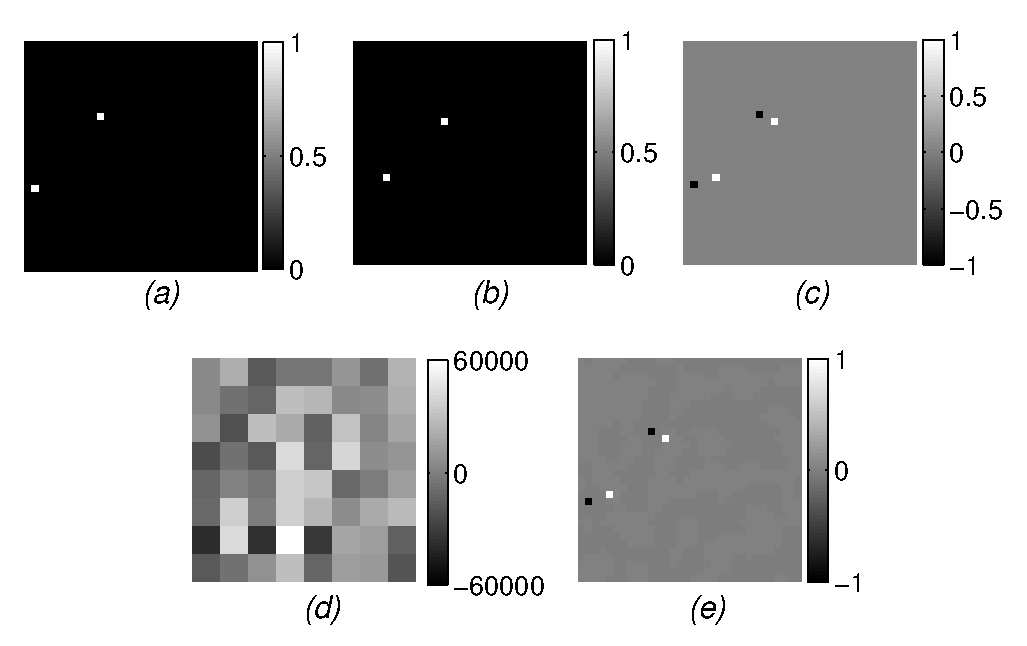
\includegraphics[scale=0.75]{scout_fig10_v2.eps}
	\captionof{figure}[Difference frame 1 of a sequence of two movers on a black background.]{A reconstruction of a $32 \times 32$ scene with two movers of equal amplitude on a black background. (a) ground-truth scene 1 (b) ground-truth scene 2 (c) ground-truth frame difference and (d) measured $8 \times 8$ frame difference, scaled so that it is discernible (e) reconstructed $32 \times 32$ difference frame}
	\label{fig:scout_fig10_un}
\end{figure}

\begin{figure}
	\centering
	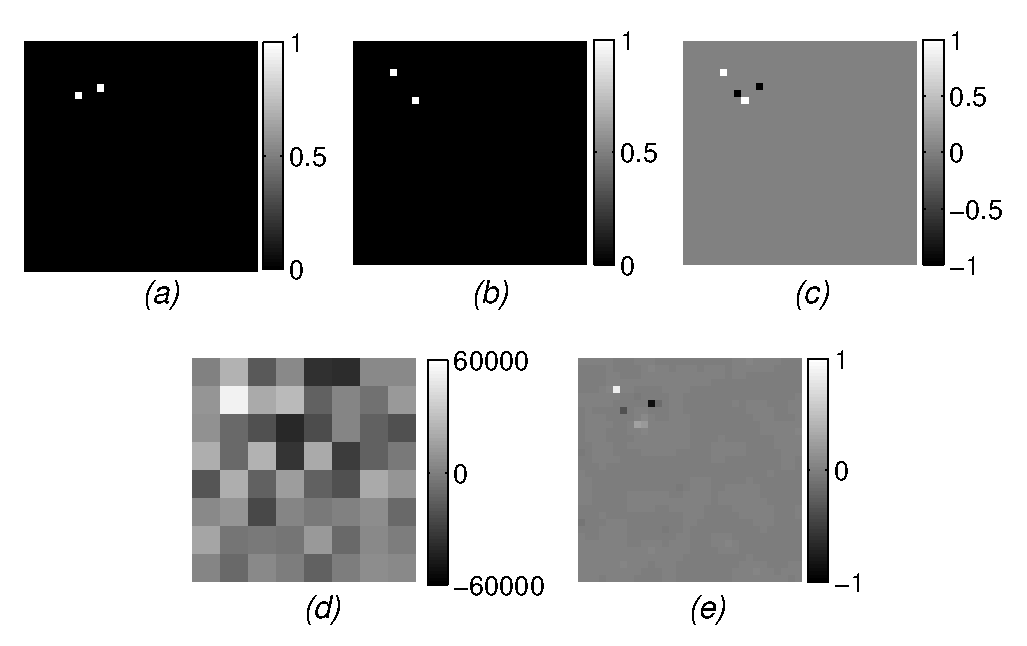
\includegraphics[scale=0.75]{scout_fig11_v2.eps}
	\captionof{figure}[Difference frame 9 of a sequence of two movers on a black background.]{A reconstruction of $32 \times 32$ scene with two movers of equal amplitude on a black background. This frame shows the results when the past and present mover locations are adjacent in the difference frame. (a) ground-truth scene 1 (b) ground-truth scene 2 (c) ground-truth frame difference and (d) measured $8 \times 8$ frame difference, scaled so that it is discernible (e) reconstructed $32 \times 32$ difference frame}
	\label{fig:scout_fig11_un}
\end{figure}


\begin{figure}
	\centering
	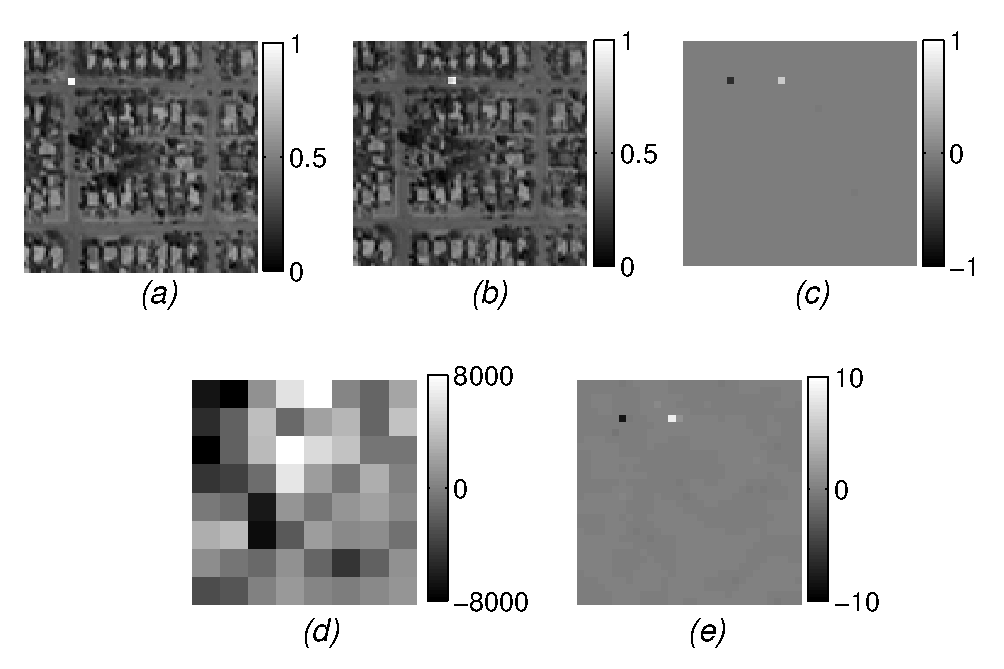
\includegraphics[scale=0.75]{scout_fig12_bg_un}
	\captionof{figure}[Difference frame 1 of a reconstruction video of two movers on a non-zero background.]{Difference frame 1 of a video demonstration of compressive tracking of a  $32 \times 32$ difference scene with a non-zero background. Scene background ©2012 Google. (a) ground- truth scene 1 (b) ground-truth scene 2 (c) ground-truth frame difference and (d) measured $8 \times 8$ frame difference, scaled so that it is discernible (e) reconstructed $32 \times 32$ difference frame}
	\label{fig:scout_fig12_bg_un}
\end{figure}


In the reconstruction of the ninth difference frame, the amplitude of one the movers had a lower amplitude, shown in \Cref{fig:scout_fig11_un}. Poor reconstruction tends to occur when two movers are located adjacent to each other in the ground-truth difference scene. This is an issue that can be traced to the system response matrix $\mb{H}$, locations next to each other have are more likely to have larger correlations in their respective \gls{psf}.


We also performed a more realistic experiment in which a mover simulates a vehicle driving on a street. This demonstrates that the \gls{scout} works well in situations with non-zero backgrounds. This sequence with the results for a single mover is also shown in Appendix \ref{app:scoutExpResults}. The first difference frame of this sequence is shown in \Cref{fig:scout_fig12_bg_un}. As seen in ground truth difference fram $\Delta \mb{f}$ shown in \Cref{fig:scout_fig12_bg_un}(c), the amplitude of the past and present mover locations in the ground-truth are lower than the zero background case. Therefore there is also less contrast in $\Delta \mb{g}$ the difference measurements in \Cref{fig:scout_fig12_bg_un}(d), which makes this case more sensitive to noise. 

The most notable feature in the non-zero background results is reduced quantitative agreement with the ground-truth, even when the calibration matrix is scaled according to \Cref{eq:ScoutCalibrationMatrixScaling}. There are several reasons for this: Nonlinearities in the overall system response that result from a nonlinear monitor “gamma” (mapping from pixel value to output brightness) and inter-pixel interactions that effect brightness. These effects are not captured during calibration as that is performed point-by-point (thus reducing inter-pixel effects) and with pixels that are fully-on or -off (thus avoiding effects from monitor gamma). Another possible reason is over-multiplexing, since the total light from each frame is increased, there is less dynamic range in the \gls{fpa}, and therefore detector non-linearity may be a source of error. Despite the lack of quantitative agreement, qualitative agreement is excellent and the movers are clearly identifiable agains the background in \Cref{fig:scout_fig12_bg_un}(e).



\section{Conclusion}

While the \gls{scout} architecture is well-suited for tracking applications, it does have limitations which make it less useful for general imaging applications. Without sparse scene motion, the priors used in reconstruction will lead to incorrect results. Reconstructions only show the locations of moving objects, and the sensing platform must be stationary relative to the scene so that frame differences are sparse. However, more sophisticated techniques could potentially estimate platform motion. Despite the limits of the \gls{scout}, the architecture is well-suited for applications such as fixed-camera wide-area surveillance where bandwidth, data volume, and cost are key concerns.

Many of the theoretical guarantees for \gls{compressive sensing} is not specialized or tuned for the block-circulant system matrix. As I mentioned in \Cref{chap:Formalism}, random coding has several theoretical properties that make them useful for compressive sensing. There has been some research work to investigate system matrices with Toeplitz and circulant structure \cite{bajwa2007toeplitz, rauhut2009circulant, romberg2009compressive}, however there has been relatively little work published discussing the approximately block-Toeplitz structure that naturally arises in optical systems such as \gls{scout} and theoretical guarantees like the ones force random coding. Two exceptions are \cite{sebert2008toeplitz, liu2008sparsesense}, which provide both theoretical evidence for the viability of CS system matrices with block-Toeplitz structure.


A completely parallel compressive imager would require as many encoding optical elements as simultaneous measurements. The \gls{scout} architecture eliminates this scaling issue by giving up the ability to implement arbitrary projections. Using a pair of masks at different distances to create a block-circulant system matrix, the system makes compressive measurements and reconstructs frame differences. The system can be optimized by adjusting system parameters such as mask pitch and defocus distance. Simulations demonstrated the use of the a modified coherence parameter as an efficient predictor of system matrix performance to optimize these parameters. An experimental system based on the \gls{scout} architecture successfully performed compressive motion tracking on scenes with zero and nonzero backgrounds in most instances. However, the reconstruction of difference scenes with adjacent mover locations caused issues due to the design or calibration of the system matrix. The system showed promising results using a general $\ell_1$ regularized least squares minimization algorithm and I believe that further research on sparse reconstruction with block-circulant system matrices may decrease reconstruction error. We also believe that non-isomorphic calibration techniques and adding further degrees of freedom in the design parameters could result in significant performance gains.





\chapter{Adaptive Feature Specific Spectral Imaging-Classifier}\label{chap:Afssic}


\section{Motivation}

Spectral imaging allows for improved discrimination of objects in a scene by measuring both spatial and spectral data \cite{chang2003hyperspectral, ibrahim2010spectral, shaw2003spectral}. By combining the spectrometer with the camera, the spectral imager produces a spectral datacube, which consists of two spatial dimensions and a spectral dimension \cite{garini2006spectral,eismann2012hyperspectral}, see \Cref{fig:isoCubes}(a).  In this chapter, I will introduce the \acrfull{afssi-c}, a computational spectral imaging system which directly classifies the spectrum at each spatial location in a scene.

One of the major limitations of \gls{isomorphic} sensing techniques in spectral imaging is due to the fact that one must acquire a three-dimensional spectral datacube using a two-dimensional \acrfull{fpa} \cite{garini2006spectral}. Traditional isomorphic systems rely on a point-by-point acquisition technique to acquire the entire spectral datacube. A \gls{whiskbroom} technique simultaneously measures the entire spectrum from a single spatial location. This is repeated for each location until the spectral datacube is completely acquired, see \Cref{fig:isoCubes}(b) \cite{wolfe1997introduction}. A \gls{pushbroom} technique measures the spectrum of an entire spatial row or column at a time, see \Cref{fig:isoCubes}(c). This is repeated until all the rows (or columns) in the spectral datacube is acquired \cite{yang2003ccd, wolfe1997introduction}. A \gls{tunable filter} technique, such as the Fabry-Perot interferometric filter \cite{fabry1897franges, perot1899application, fabry1901new}, simultaneously measures a single spectral channel  over the entire \gls{fov}, scanning through the spectral dimension, see \Cref{fig:isoCubes}(d) \cite{gat2000imaging}. 

\begin{figure}[htb]
	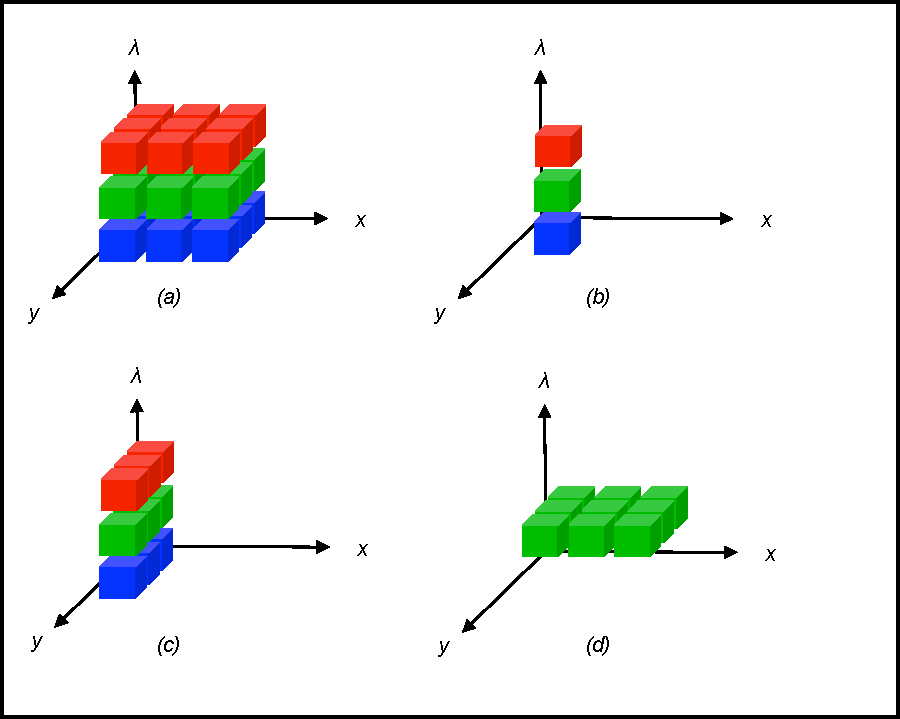
\includegraphics[scale=1.0]{isoCubes}
	\captionof{figure}[Discrete representation of the spectral datacube and various scanning measurement techniques]{(a) A discrete spectral datacube with $R_x = 3, R_y = 3, N_{\lambda} = 3$. (b) The whiskbroom technique measures the entire spectrum one spatial location at a time. (c) The pushbroom technique measures the entire spectrum on an entire spatial row or column at a time. (d) The tunable filter technique measurements an entire monochromatic image one spectral channel at a time.}
	\label{fig:isoCubes}
\end{figure}


The problem with the traditional ismorphic technique is that a typical spectral datacube has a significant amount of measurement samples. The \acrfull{aviris} system, acquires $R_x \times R_y = 677$ spatial locations (pixels) and $N_{\lambda} = 224$ spectral channels \cite{green1998imaging}, producing a spectral datacube with $N \approx 10^9$ measurement samples in $10$ minutes. 

Just like with the traditional spectrometer and camera, researchers have turned \gls{computational sensing} for spectral imaging. These architectures use the \gls{Fellgett advantage} (multiplexing) and \gls{Jacquinot advantage} (open aperture) to improve the \acrfull{snr} and reduce acquisition time and use a computational step to solve an inverse problem to reconstruct the spectral datacube \gls{spectralDataCube} from non-isomorphic measurements. Some spectral imaging architectures also leverage \gls{compressive sensing}. 

One of the early examples of computational sensing in spectral imaging is the \gls{ctis} \cite{descour1995computed}, see \Cref{fig:ctisArch}. The \gls{ctis} can reconstruct the spectral datacube \gls{spectralDataCube} from a single \gls{fpa} exposure by recording multiple measurements of the spectral datacube simultaneously. The \gls{ctis} uses several gratings to create two-dimensional projections of the three-dimensional hyperspectral datacube, see \Cref{fig:CTIS}. According to the central slice theorem, the two-dimensional Fourier Transform of each projection is a plane through the three-dimensional frequency space representation the spectral datacube. Ideally, one must collect enough projections to fully reconstruct the three dimensional frequency representation of the spectral datacube. The three-dimensional real-space distribution of the spectral datacube is then recovered through an inverse three-dimensional Fourier transform. This is similar to how computed tomography medical imaging works. However, in practice only a finite subset of projections are recorded and missing information is must be inferred. In the \gls{ctis}, the missing information is recovered by maximizing the likelihood of the measurement data using the expectation-maximization algorithm \cite{steven1993fundamentals, moon1996expectation}. According to the practical definition of compressive sensing, the \gls{ctis} maybe considered a compressive sensing technique since the number of measurement samples is less than the object dimensionality of the spectral datacube. However, it does not take advantage of sparsity or incoherence in order to reconstruct the spectral datacube.

\begin{figure}
	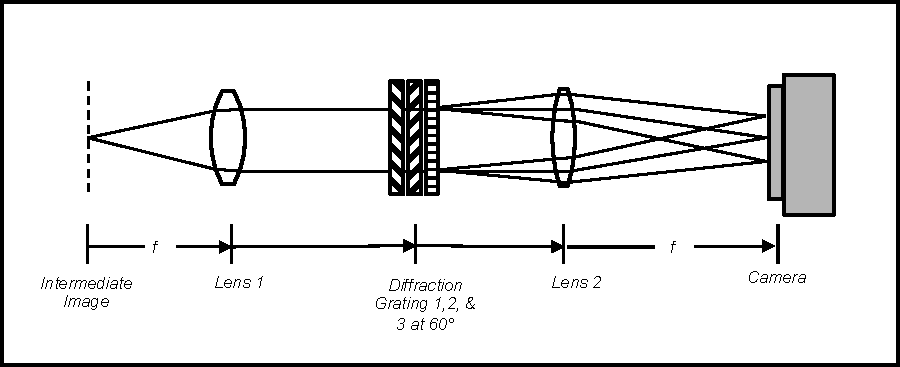
\includegraphics[scale=1.0]{ctisArch}
	\captionof{figure}[The architecture of the \acrfull{ctis}.]{The architecture of the \acrfull{ctis} consists of a collimating lens, several diffraction gratings, an imaging lens, and a \acrfull{fpa}. Each diffraction grating produces three two-dimensional projections of the three-dimensional spectral datacube (Two first order and one zeroth order). In this example,  gratings are rotationally seperated by 60 degrees to produce multiple projections. \cite{descour1995computed}}
	\label{fig:ctisArch}
\end{figure}

\begin{figure}
	\centering
	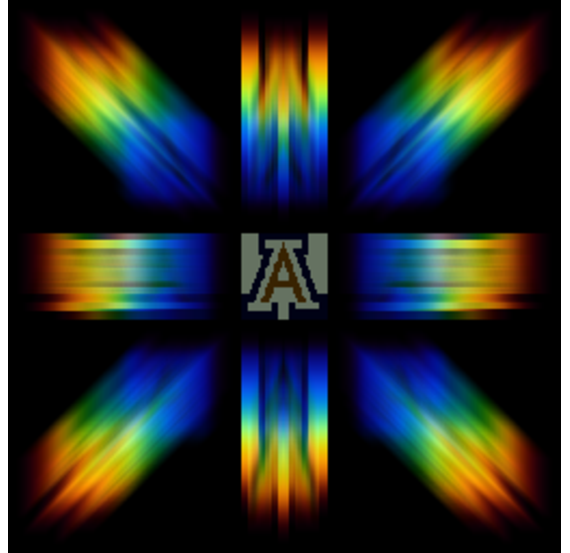
\includegraphics[scale=1.0]{CTIS.pdf}
	\captionof{figure}[The optical image before being sampled by the \gls{fpa} in the CTIS]{The optical image before being sampled by the \gls{fpa} in the \gls{ctis}. The \gls{ctis} uses multiple gratings to create projections of the spectral datacube at the \gls{fpa}. Note the center image is the zeroth order and is simply the undiffracted color image of the object scene \cite{descour1995computed}.}
	\label{fig:CTIS}
\end{figure}

In another example of computational sensing applied to spectral imaging is the \acrfull{cassi} sensor, see \Cref{fig:cassiArch}. In the \gls{cassi}, a coded aperture spatially codes the spectral datacube \gls{spectralDataCube}. The dispersive element then creates a projection of the spectral datacube that maps three-dimensional information into a two-dimensional image at the \gls{fpa}. Unlike the \gls{ctis}, only one two-dimensional projection is recorded per \gls{fpa} image which allows for higher spatial resolution for the same detector array. Using calibration data and prior knowledge of sparsity, the post-processing step solves the \gls{lasso} problem to reconstruct the spectral datacube \cite{wagadarikar2008single, arce2014compressive}. Often a total-variation regularization is also invoked to improve reconstruction of the spatially varying image \cite{wagadarikar2008spectral, bioucas2007new}.


\begin{figure}
	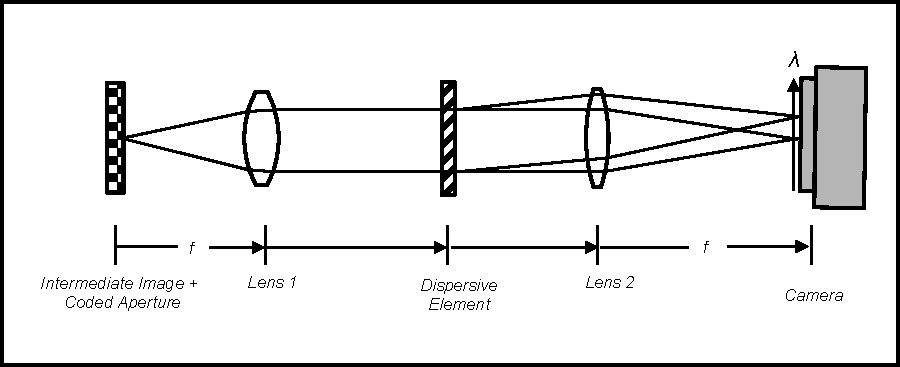
\includegraphics[scale=1.0]{cassiArch}
	\captionof{figure}[The architecture of the \acrfull{cassi}.]{The architecture of the \acrfull{cassi} consists of a collimating lens, a disperive element, an imaging lens, and a \acrfull{fpa}. The coded aperture spatially codes each wavelength layer in the three-dimensional spectral datacube. Then the dispersive element creates a wavelenght depedent spatial shift, shearing the spectral datacube. The monochromatic image of the \gls{fpa} creates a coded two-dimensional projection of the three-dimensional spectral datacube.}
	\label{fig:cassiArch}
\end{figure}


All traditional and computational spectral imaging architectures including the \gls{ctis} and the \gls{cassi} only reconstruct the spectral datacube \cite{hagen2013review}. This produces a significant amount of data, which is only used as an intermediate step. One is typically interested in determining the which chemical or material is responsible for a spectrum at a specific location. This is called spectral classification \cite{chang2003hyperspectral, dupont2011spatial, liu2014discriminative}. Therefore, an additional post-processing step needed. If however, one could directly classify the spectrum ,one could signficantly reduce the amount of data storage and communication resources required to operate the instrument. 

Previously my colleuges developed a computational spectrometer called the \acrfull{afss} \cite{dinakarababu2011adaptive}. Shown in \Cref{fig:afssArch}, the \gls{afss} was the first experimental computational sensor that make use of an adaptive scheme which uses measurement data to design spectral filters (codes). This allowed the spectrometer to directly classify the chemical or material responsible for the spectrum without the need to perform a reconstruction step. By combining the \gls{Fellgett advantage} with an adaptive algorithm to create custom spectral filters, the \gls{afss} was able to demonstate significant reduction in the number of measurements to classify a spectrum compared to non-adaptive multiplexed spectrometers in low \gls{snr} scenarios. In this context, the spectral filters act as feature vectors, which are computed using variation of \gls{pca}.\footnote{In the context of the AFSS and AFSSI-C the terms spectral filter, code, and feature vector are synonymous.}

The \acrfull{afssi-c} extends the concept first demonstrated by the \gls{afss} to spectral imaging. The \gls{afssi-c} directly classifies the spectrum at each spatial location without the need to reconstruct the spectral datacube. By adopting a task-specific sensing approach, the \gls{afssi-c} greatly improves classification accuracy while simultaneously reduces the amount of bandwidth and storage for data. Furthermore, the architecture of the \gls{afssi-c} leverages both the Fellgett and adaptive measurement scheme like the \gls{afss}, while also adding the Jacquinot advantag to outperform all traditional and currently known computational spectral imaging instruments in terms of number of measurements to correct classifcation.

\section{Architecture}

I want to quickly review the architecture of the \acrfull{afss} before discussing the architecture of the \gls{afssi-c}. The \gls{afss}, shown in \Cref{fig:afssArch}, is the earliest known computational spectrometer to use adaptive spectral filters to classify spectra \cite{dinakarababu2011adaptive}. Unlike the traditional slit spectrometer, the \gls{afss} images the dispersed slit onto a \gls{dmd}. The mirrors of the \gls{dmd} can then be adjusted to selectively reflect certain wavelengths towards the condensor lens, which then focuses light onto a single detector element \cite{dinakarababu2011adaptive}. By reflecting or ``turning on'' multiple \gls{dmd} mirrors and only using a single detector element, we achieved the \gls{Fellgett advantage}. By using measurement data to actively design spectral filters, the \gls{afss} outperforms non-adaptive schemes by eliminating spectra that improbable and turns it attention towards trying to classify the remaining high probability spectra. 

\begin{figure}
	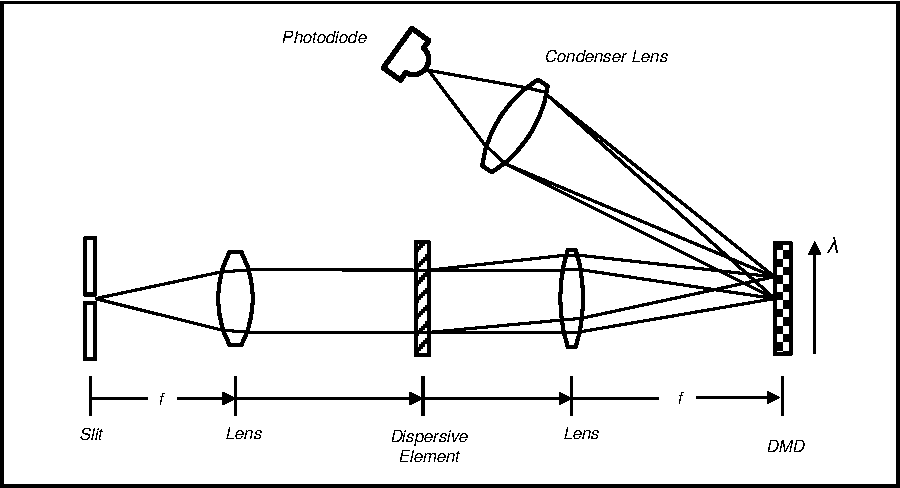
\includegraphics[scale=1.0]{afssArch}
	\captionof{figure}[The architecture of the Adaptive Feature Specific Spectrometer. ]{The slit blocks light from all but one spatial location. A lens collimates the light passed from the slit and a dispersive element creates monochromatic images of the slit at different columns on the \gls{dmd}, corresponding to different spectral channels. The \gls{dmd} can then selectively reflectives combinates of each spectral channels into the condenser lens. The condensor lens focuses all the light onto a single detector element, a photodiode.}
	\label{fig:afssArch}
\end{figure}

In order to create an imaging version of the \gls{afss}, one may naively attempt to extend the \gls{afss} architecture by forming a parallel array of \gls{afss} sensors to achieve classification across a spatial scene. However, just like in the proposed parallel single-pixel camera design in \Cref{chap:Scout}, this approach would significantly increase the \gls{swap-c} of the design. The \gls{afssi-c} provides a similar feature-based measurement approach and Bayesian framework but with a more compact architecture. Rather than a fully parallel version of the \gls{afss}, the optical design of the \gls{afssi-c} uses a single \gls{dmd} and a single set of lenses and dispersive elements sharing a common entrance pupil. This approach share resources across multiple spatial locations.


\begin{figure}
	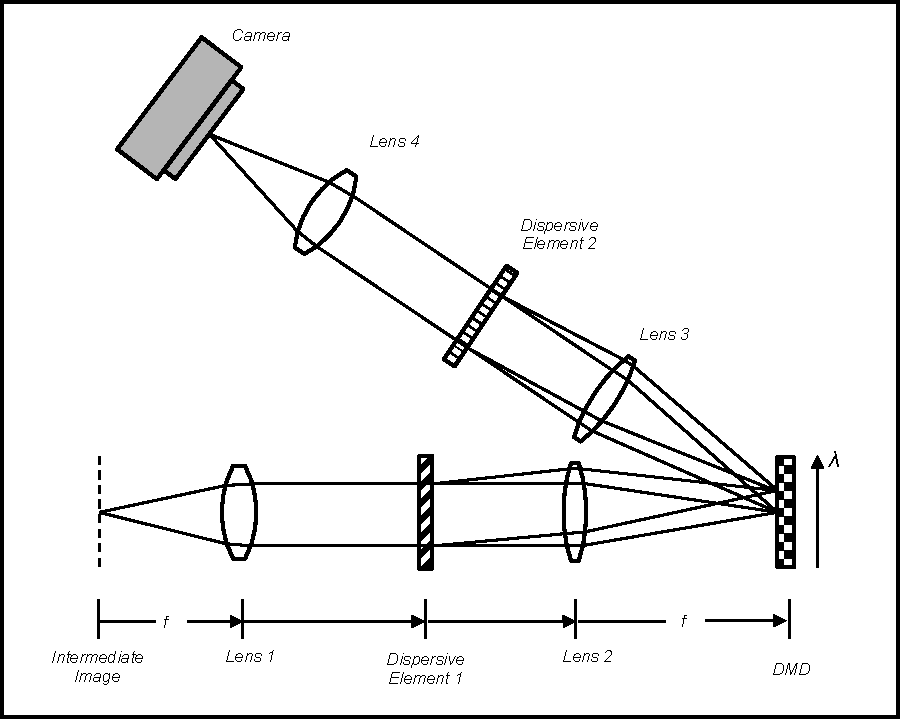
\includegraphics[scale=1.0]{afssicArch}
	\captionof{figure}[The architecture of the Adaptive Feature Specific Spectral Imaging-Classifier]{An objective lens forms the intermediate image of the object scene at the input plane of the instrument. The first lens collimates the light and a diffraction grating disperses the light. A second lens images spectrally dispersed versions of the image of the object scene onto the \gls{dmd}. The \gls{dmd} directs light to a beam dump or reflects the light towards the third lens on a mirror-by-mirror basis. Collimated light from third lens
is sent through a second grating, and finally imaged onto the detector by the fourth lens.}
	\label{fig:afssicArch}
\end{figure}


The design of the \gls{afssi-c} is essentially two 4\textit{f} open-aperture monochromators seperated by a \acrfull{dmd}, shown in Fig.~\ref{fig:afssicArch}. In our experiment, we used an objective lens, which is not shown, to create an intermediate image at the input plane of the instrument. At this point in the system one can imagine the source spectral datacube as depicted in \Cref{fig:sysCubes}(a), where $x$ and $y$ are the spatial axes, and $\lambda$ the spectral axis. The first lens of the system collimates the light from the input place. The first grating disperses the light. The second lens then images spectrally dispersed copies of the intermediate image on the \gls{dmd}. Just prior to being reflected from the \gls{dmd}, one can imagine the spectral dimension of the datacube as being sheared at an angle, in the direction of the dispersion, see \Cref{fig:sysCubes}(b). As in the \gls{afss}, each mirror on the \gls{dmd} either reflects light into the second arm or reflects light away into a beam dump (not shown). One can visualize this by looking at \Cref{fig:sysCubes}(c), a mirror that reflects light away, towards the beam dump, deletes columns in the sheared spectal datacube. The light that reflected into the second arm is then collimated before hitting the second grating, which is identical to the first, but with the reverse dispersion direction. This removes the shear in the encoded spectral datacube, seen in \Cref{fig:sysCubes}(d). Lens 4 images the unsheared spectral datacube onto the \gls{fpa}. The grayscale image of the \gls{fpa} essentially integrates the spectral datacube over the spectral dimension. 

\begin{figure}
	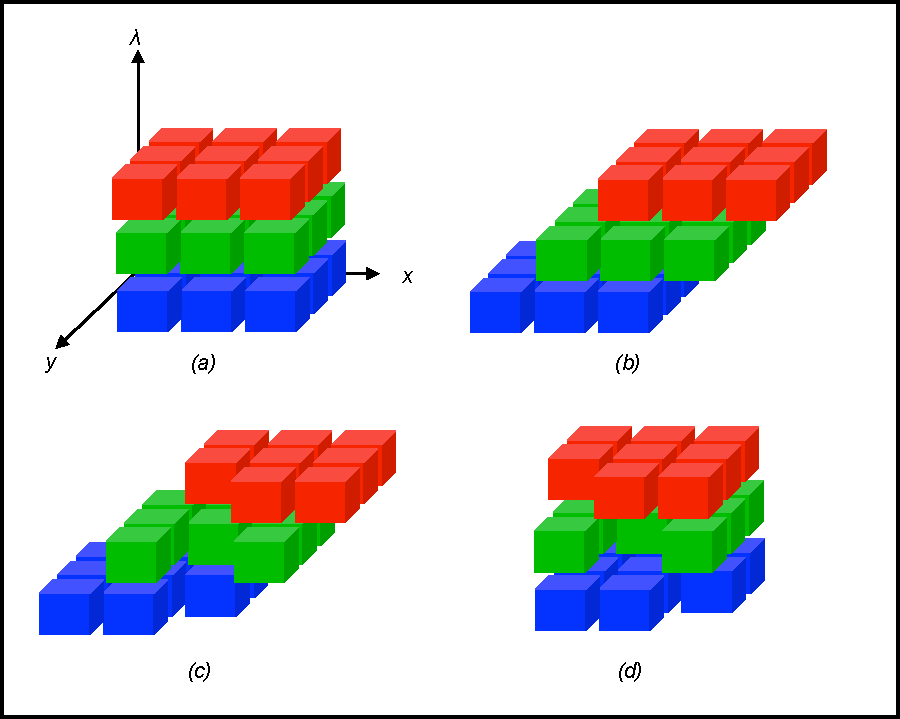
\includegraphics[scale=1.0]{justCubes}
	\captionof{figure}[Visualization of datacube progression through the \gls{afssi-c} system.]{(a) The input cube is (b) sheared by the first grating, (c) encoded at the \gls{dmd}, and finally (d) spatially re-registered by the second grating.}
	\label{fig:sysCubes}
\end{figure}

We choose to use a dual-disperser architecture rather than the single-disperser architecture such as the one in the \gls{cassi} since the mirror patterns on the \gls{dmd} acts as spectral filters for each spatial location. In the dual-disperser design, the spectral coding of each spatial location is more straightforward and elegant approach for parallel direct classification: the architectures allows us to write the image of each \gls{fpa} pixel as an innner product of the spectrum at the corresponding location at the source with the spectral filter created by the \gls{dmd}, allowing for parallel operation of the Bayesian inference approach. A single-disperser design would entangle both the spectral and spatial dimension of the spectral datacube, and would require solving a single larger joint inference problem.

\subsection{Forward Model}

Imagine a continuous spectral datacube which we call the source spectral density of $D_0 \left(x, y;\lambda \right)$ at the input aperture. To simplify the forward model analysis, assume unit magnification and ignore diffraction, aberrations, and vignetting. The spectral density just before reflection from the \gls{dmd} is written as:
%
\begin{equation}
\begin{split}
		D_1 \ap{ x, y; \lambda } & = \iint \delta \ap{x^\prime - \left[ x + \alpha \ap{\lambda - \lambda_c} \right] } \delta \ap{y^\prime - y } D_0 \ap{x^\prime, y^\prime; \lambda} dx^\prime dy^\prime \\
		& = D_0 \ap{x + \alpha \ap{\lambda - \lambda_c}, y; \lambda}
\end{split}
\end{equation}
%
Notice that this can thought of as a two-dimensional convolution of the spectral density with an wavelength dependant \acrfull{psf} that shifts the spectral density by an amount $\alpha \ap{\lambda - \lambda_c}$, where $\alpha$ is the dispersion and $\lambda_c$ is the center wavelength. If there is no dispersion, when $\alpha = 0$, then one would get the original spectral density back. Note, that when $\lambda = \lambda_c$ there is no shift in the $x$ direction. 

After reflecting from the \gls{dmd} the spectral density can then be written as:
%
\begin{equation}
D_2 \ap{ x, y; \lambda } = T\left( x, y \right) D_1\ap{ x, y; \lambda} = T \ap{ x, y } D_0 \ap{x + \alpha \ap{\lambda - \lambda_c}, y; \lambda}
\end{equation}
%
where $T \ap{ x, y }$ represents the reflection pattern of the \gls{dmd}. If $T = 1$ the light is being reflected into the second arm and if $T = 0$ the light is being reflected towards the beam dump. 

Propagating through the second arm has the effect of reversing the shear imposed on the spectral density:
%
\begin{equation}
\begin{split}
	D_3 \ap{x,y;\lambda} & = \iint  \delta \ap{x^\prime - \left[ x - \alpha \ap{\lambda - \lambda_c} \right]} \delta \ap{y^\prime - y} D_2 \ap{x,y;\lambda} dx^\prime dy^\prime \\
	& = T \ap{x - \alpha\ap{\lambda - \lambda_c},y} D_0 \ap{x,y;\lambda} \\
	& = H \ap{x,y;\lambda} D_0 \ap{x,y;\lambda}
	\label{eq:afssicFilter}
\end{split}
\end{equation}
%
Notice that the dispersion $\alpha$ has the opposite sign. This equation is represented in discrete form in \Cref{fig:sysCubes}(d). Thus, propating through the entire optical system represents multiplying the input spectral density with a spectral desnity filter function $H \ap{x,y;\lambda}$. 

Since the \gls{fpa} image is grayscale, ignoring quantization effects, the image can be written as an integral over the wavelengths
%
\begin{equation}
	I\ap{x,y} = \int H \ap{x,y;\lambda}  D_0 \ap{x,y;\lambda} d\lambda
\end{equation}
%
By taking into account the spatially pixeled detector array with pixel size $\Delta$, then the discrete \gls{fpa} image is
%
\begin{equation}
	\Gamma_{nl} = \iiint \mbox{rect} \ap{ \frac{x}{\Delta} - n, \frac{y}{\Delta} - l } H \ap{x,y;\lambda} D_0 \ap{x,y;\lambda} dx^\prime dy^\prime d\lambda
	\label{eq:afssicDiscreteReadout}
\end{equation}
%
where $\Gamma_{nl}$ is the image value from the $n^{th}$ and $l^{th}$ location. Now consider that the \gls{dmd} pattern $T$ is also pixelated with the same pixel size $\Delta$ as in the detector. 
%
\begin{equation}
	T \ap{x,y} = \sum_{n^\prime, l^\prime}  T_{n^\prime, l^\prime} \mbox{rect} \ap{ \frac{x}{\Delta} - n^\prime, \frac{y}{\Delta} - l^\prime}
	\label{eq:afssicDiscreteDMD}
\end{equation}
%
Inserting \Cref{eq:afssicDiscreteDMD} into \Cref{eq:afssicFilter} and \Cref{eq:afssicDiscreteReadout} produces a single equation which describes how the signal-of-interest $D_0 \left( x, y; \lambda \right)$ is measured by the \gls{afssi-c}:
%
\begin{align} \label{eq:PixelizedDetectIntensity}
	\Gamma_{nl} &= \sum_{n^\prime l^\prime} \iiint \mbox{rect} \left( \frac{x}{\Delta} - l, \frac{y}{\Delta} - n \right) \mbox{rect} \left( \frac{x-\alpha \left(\lambda - \lambda_c\right)}{\Delta} - l^\prime , \frac{y}{\Delta} - n^\prime \right) \notag \\
 	&\qquad \times T_{n^\prime l^\prime} D_0 \left( x, y; \lambda \right) dx \, dy \, d\lambda.
\end{align}
%
This equation maybe somewhat difficult to interpret, so to add some additional intuition I will go through an example of a monochromatic source at the center wavelength, $D_0 \left(x, y, \lambda\right) = I_0 \left(x, y \right) \delta \left( \lambda - \lambda_c \right)$, where $I_0$ is the intensity distribution of the monochromatic scene. In this case, \Cref{eq:PixelizedDetectIntensity} simplifies to
%
%
\begin{align} \label{eq:MonoChrome}
	\Gamma_{nl} \left(\lambda = \lambda_c \right) &= \sum_{ n^\prime l^\prime} \iiint \mbox{rect} \left( \frac{x}{\Delta} -  l, \frac{y}{\Delta} - n \right)  \mbox{rect} \left( \frac{x}{\Delta} - l^\prime, \frac{y}{\Delta} - n^\prime \right) \notag \\
	&\qquad \times T_{n^\prime l^\prime} I_0 \left( x, y \right) \delta \left( \lambda - \lambda_c \right) dx \, dy \, d\lambda  \notag \\
	%
	&= \sum_{ n^\prime l^\prime} T_{n^\prime l^\prime}  \iint \mbox{rect} \left( \frac{x}{\Delta} -  l, \frac{y}{\Delta} - n \right)  \mbox{rect} \left( \frac{x}{\Delta} - l^\prime, \frac{y}{\Delta} - n^\prime \right) \notag \\
	&\qquad \times I_0 \left( x, y \right) dx \, dy \, \int \delta \left( \lambda - \lambda_c \right)d\lambda  \notag \\
	%
 	&= \sum_{n^\prime l^\prime} \delta_{ll^\prime} \delta_{nn^\prime} T_{n^\prime l^\prime} I_{nl} \notag \\
 	&= T_{nl} I_{nl},
\end{align}
%
where $I_{nl}$ is a spatially pixelated version of the monochromatic source with intensity distribution $I_0 \left(x, y \right)$. One now sees that in the monochromatic case, the measurement is point-by-point multiplication of the \gls{dmd} pattern with the discrete monochromatic image $I_{nl}$

In the next example, I consider the case where a monochromatic source is not at the center wavelength but is shifted in wavelength. The wavelength of the monochromatic source is shifted from the center wavelength by a single spectral channel $\lambda= \lambda_c + \Delta_{\lambda}$, where $ \Delta_{\lambda} = \Delta / \alpha$. The spectral density is now written as $D_0 \left(x, y, \lambda\right) = I_0 \left(x, y \right) \delta \left( \lambda - \ap{\lambda_c + \Delta_{\lambda} } \right)$. \Cref{eq:PixelizedDetectIntensity} simplifies to
%
\begin{align} 
	\Gamma_{nl}\left(\lambda = \lambda_c + \Delta \lambda\right) &= \sum_{n'l'} \iiint \mbox{rect} \left( \frac{x}{\Delta} - l, \frac{y}{\Delta} - n \right)  \mbox{rect} \left( \frac{x}{\Delta} - \left(l' + 1 \right), \frac{y}{\Delta} - n' \right) \notag \\
 	&\qquad \times T_{n'l'} I_0 \left( x, y \right) \delta \left( \lambda - \left( \lambda_c + \Delta \lambda \right)\right) dx \, dy \, d\lambda  \notag \\
 	%
	&= \sum_{ n^\prime l^\prime} T_{n^\prime l^\prime}  \iint \mbox{rect} \left( \frac{x}{\Delta} -  l, \frac{y}{\Delta} - n \right)  \mbox{rect} \left( \frac{x}{\Delta} - \left(l' + 1 \right), \frac{y}{\Delta} - n' \right) \notag \\
	&\qquad \times I_0 \left( x, y \right) dx \, dy \, \int \delta \left( \lambda - \left( \lambda_c + \Delta \lambda \right)\right) d\lambda  \notag \\
	%
 	&= \sum_{n'l'} \delta_{l \left( l' + 1 \right) } \delta_{nn'} T_{n' l'} I_{nl} \notag \\
 	&= T_{n\left(l - 1 \right)} I_{nl}
 	\label{eq:Mono2}
 \end{align}
%
This shows that a shift by one spectral channel results in a shift of one pixel in of the \gls{dmd} pattern.

Using the intuition from the last two examples, I will now extend this to a non-monochromatic case. Consider spectral channel index \gls{specchan} out of \gls{numspecchan} total spectral channels.
We can also define a discretized source spectral datacube $D_{nlc}$, and then the detector signal $\Gamma_{nl}$ as a result of mirror pattern $T$ acting on the pixelated source is
%
%
\begin{equation}
	\Gamma_{nl} = \sum^{N_{\lambda}-1}_{c = 0} T_{n \left( l + c \right)} S_{nlc},
\end{equation}
%
%
which shows the measurement at each pixel being the inner product of the source spectrum and the spectral filter which results from the mirror pattern. If one inspects the adjacent pixel on the detector, $\Gamma_{n \left(l +1 \right)}$ we find that
%
%
\begin{equation}
\Gamma_{n\left(l-1\right)} = \sum^{N_{\lambda}-1}_{c = 0} T_{n\left( l + 1 + c \right)} S_{n\left(l+1\right)c}.
\end{equation}
%
%
The spatial location $\left(n,l \right)$ sees the effect of the pattern in mirror locations $T_{nl}$ to $T_{n\left(l+N_{\lambda}-1\right)}$, while the neighboring spatial location at $n, \left( l + 1\right)$ is encoded by the mirror pattern from $T_{n\left(l+1\right)}$ to $T_{n\left(l + N_{\lambda} \right)}$. Notice that given two neighboring spatial pixels in the input aperture, $l$ and $l+1$, mirror pixels $T_{n\left( l + 1 \right)}$ to $T_{n\left(l + N_{\lambda} - 1 \right)}$ are common to both locations. 

Now the design constraint of the \gls{afssi-c} architecture is clear, while a naively parallel set of \gls{afss} would have been costly in terms of \gls{swap-c}, using a common entrance pupil prevents indepdent spectral filters for each spatial location. The spectral filters imposed by the \gls{dmd} pattern maybe unique for every spatial location, but \textit{cannot} be implemented independently, requiring the features to be designed \textit{jointly} for spatial locations along a row (the $l$ direction).



\section{Adaptive Classification Algorithm}

As mentioned earlier, the \gls{afssi-c} uses adaptive features to directly classify the spectrum at each spatial location. At each measurement step $m$, the classification algorithm computes the probability of each hypothesis spectra in a spectral library. Building on the discussion of \acrfull{pca} and Bayesian statistics in \Cref{chap:Formalism}, I will discuss how the classification algorithm of the \gls{afssi-c} works. 


Since the \gls{afssi-c} feature vectors are not indpendent for each spatial location, it is more intuitive to discuss the algorithm when only a single spatial location exist in the spectral datacube. The reader can then expand the intuition to the entire scene. For a single pixel architecture, one can write the discrete forward model as
%
\begin{equation}
g_m = \mb{t}_{m}^{T} \mb{f}
\end{equation}
%
where $g_m$ is the $m^{th}$ measurement of \gls{dmd} mirror pattern $\mb{t}_m$ and $\mb{f}$ is the ground truth spectrum of the source. 

The measurement from the detector is compared to the spectral library, subject to the spectral filter implemented at that spatial location. A probability is assigned to each hypothesis in the spectral library using Bayes' theorem. The conditional probability of the hypothesis, which is spectrum $\mb{s}_i$ is present, given the measurement history up to the $m^{th}$ measurement $\{g\}_m$, can be written as:
%
\begin{equation}\label{eq:BayesThm2}
\mbox{P} \left( h_i | \{ g \}_m \right) = \frac{\mbox{P} \left( \{g\}_m |\, h_i \right) \; \mbox{P} \left(h_i\right)}{\mbox{P} \left( \{g\}_m \right)}.
\end{equation}



Remember from Chapter 2, that \gls{pca} provides the optimal basis to distinguish between data vectors in a vector space by diagonalizing the covariance matrix. The covariance matrix (or scatter matrix) is simply the matrix multiplication of the spectral library (with the mean spectrum subtracted) with the transpose of itself. 

\begin{align}
\textbf{Q} &= \sum^{N_{R}}_{r \;= \,1} \left(\textbf{s}_r - \bar{\textbf{s}} \right) \left(\textbf{s}_r - \bar{\textbf{s}} \right)^T \notag \\
&=\textbf{X}\;\textbf{X}^T. \label{eq:nonweightedScatter}
\end{align}

However, since the spectral library is constant with respect to the measurements, the set of principal components will also remain constant. Intuitively, one can use the probability of each spectrum that was computed from the last measurement to weight each of the spectra in the library. Geometrically, one can imagine that the direction of largest variation is now biased to align in the direction with higher probability spectra. The geometric depiction of the probabilistically weighted \acrfull{pca} which we call pPCA is shown in \Cref{fig:pPCA}.

%
\begin{figure}[htb]
  \centering
  % Requires \usepackage{graphicx}
  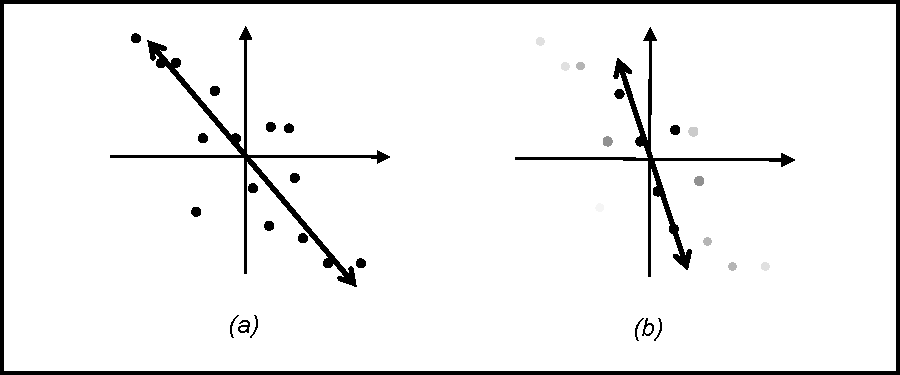
\includegraphics[scale=1.0]{pPCA}
  \caption{Depiction of the pPCA (simple 2D example). (a) First principal component before a measurement has been made. All of the hypotheses are equiprobable, depicted here as all points having the same grayscale value. (b) After a measurement has been made: the darker points are more probable hypotheses, with the less probable hypotheses taking on lighter shades of gray. The first principal component has now been shifted to the direction of greatest variation in the weighted data.}\label{fig:pPCA}
\end{figure}
%
I will now go over the formalism for \gls{ppca}. At each spatial location, we create a covariance matrix with \gls{numspeccand} spectral hypotheses, with individual spectrum $\textbf{s}_r$, weighted in relation to the prior probability associated with each hypothesis given the measurement history. The individual covariance matrices $\textbf{{Q}}(m)$ at each spatial location with spectral library element hypothesis $h_r$ take the form
%
%
\begin{align}
\textbf{Q}(m) &= \sum^{N_{\lambda}}_{r \;= \,1} \mbox{P} \left( h_r | \{g\}_m \right) \left(\textbf{s}_r - \bar{\textbf{s}} \right) \left(\textbf{s}_r - \bar{\textbf{s}} \right)^T \notag \\
&=\textbf{X}(m)\;\textbf{X}^T(m). \label{eq:preScatter}
\end{align}
%
%
Here $\textbf{X}(m)$ is the matrix of weighted spectral elements, where the row index $i$ is from 1 to the number of spectral channels $N_{\lambda}$; the columns $r$ from 1 to \gls{numspeccand} as follows,
%
%
\begin{equation}
	\textbf{x}_{r}(m) = \sqrt{\mbox{P} \left(h_r \vert \{g\}_m \right)} \left(\mb{s}_{r} - \bar{\textbf{s}}\right),
\end{equation}
%
%
and $\bar{\textbf{s}}$ is the probabilistically-weighted sum of the spectral library:
%
%
\begin{equation} \label{eq:Sbar}
\bar{\textbf{s}} = \sum^{N_R}_{r \;= \, 1} \mbox{P} \left( h_r | \{g\}_m \right) \textbf{s}_r.
\end{equation}


We can then compute the first eigenvector of $\textbf{Q}(k)$, analogous to PCA. We call this probabilistic-PCA or pPCA, and in the case of the AFSS this eigenvector becomes the feature for the next measurement. The scatter matrix $\textbf{Q}(k)$ is then updated with every measurement.

\subsection{Updating Probabilities}\label{ssec:updatingProbabilities}

In practice we do not directly compute the posterior probabilities for each hypothesis using Bayes' theorem, \Cref{eq:BayesThm2}, since we have no meaningful way of computing the probability of the measurement history $\prob{ \{g\}_m }$. Thankfully, the method of \acrfull{map} and taking ratios of posterior probabilities that I discussed in Chapter 2 allows one to compute relative probabilities which will be used to weight the spectral library after each measurement. For now I will define the ratio of the posterior probabilities
%
\begin{equation}
	  L_{ij}^{\left\{ g \right\}_m} := \pr{h_i | \{g\}_{m} }{h_j | \{g\}_{m} } = \pr{ \{g\}_{m}|h_i }{ \{g\}_{m}|h_j} \pr{h_i}{h_j}
	  \label{eq:initRatio1}
\end{equation}
%
where $\{g\}_{m}$ is the set of all measurements, including the current measurement number index $m$.


Note that if we assume that the likehood probabilities are indepdent, then we can write the joint probability as a product of the likelihood of the current measurement with the likelihoods of all past measurements
%
\begin{align}
	\prob{\{g\}_m|h_i} &= \prob{g_m|h_i} \prob{\{g\}_{m-1}|h_i} \notag \\
							&= \prob{g_m|h_i} \prod_{m'=1}^{m-1} \prob{g_{m'}|h_i}
\end{align}
So we can expand \Cref{eq:initRatio1} 

\begin{equation}
	  L_{ij}^{\left\{ g \right\}_m} =  \frac{ \prob{g_m|h_i} \prod_{m'=1}^{m-1} \prob{g_{m'}|h_i} }{ \prob{g_m|h_i} \prod_{m'=1}^{m-1} \prob{g_{m'}|h_j}} \pr{h_i}{h_j}
	  \label{eq:initRatio2}
\end{equation}
%
If I define
%
\begin{equation}
L_{ij}^{\left\{ g \right\}_{m-1}} := \frac{ \prod_{m'=1}^{m-1} \prob{g_{m'}|h_i} }{ \prod_{m'=1}^{m-1} \prob{g_{m'}|h_j}} \pr{h_i}{h_j}
\end{equation}
%
then \Cref{eq:initRatio2} simplifies into
%
\begin{equation}
	  L_{ij}^{\left\{ g \right\}_m} =  \frac{ \prob{g_m| h_i} } { \prob{g_m| h_j} } L_{ij}^{\left\{ g \right\}_{m-1}}
	  \label{eq:initRatio3}
\end{equation}
%
This equation provides a convient way to update the ratio of posterior probabilities after each measurement.

The question now turns to how does one actually compute the likelihoods. For this step we assumed that the likelihood takes on a Gaussian noise model with standard deviation of the noise $\sigma_{\text{AWGN}}$. Thus we say the probability of the measurement $g_m$ given that hypothesis $h_i$ is true is 
%
\begin{equation}
	\prob{g_m | h_i } = \frac{1}{\sqrt{2\pi\sigma_{\text{AGWN}}^2 }} 
	\exp \left[ - \frac{ \ap{g_m - \mb{t}_m \cdot \mb{s}_i } }{2 \sigma_{\text{AGWN} }^2} \right]
	\label{eq:noiseModel1}
\end{equation}
%
where $\mb{t}_m$ is the spectral filter at the measurement step $m$. This equation means that when the measurement value $g_m$ is close to the inner product of the spectral filter and the hypothesis spectrum, the probability is large. As the measurement value deviates from $\mb{t}_m \cdot \mb{s}_i $ the probability decreases.

After each measurement we compute \Cref{eq:initRatio3} for all pairs of spectra ${i,j}$ using the noise model \Cref{eq:noiseModel1}. In practice, the exponentials of numbers of moderate size cause numerical issues. To avoid this, we compute the logarithm of the likelihood (log-likelihood) ratios to eliminate the exponentials. In Appendix \ref{app:Derivation of the LLR Update}, I will discuss the update rule using log-likelihood ratios. 

\subsection{Extension to Spectral Imaging}

In the case of spectral classification for only a single spatial location, like the \gls{afss}, the number of \gls{dmd} mirrors is equal to the number of spherical channels. 
%
\begin{equation}
	N_d = N_{\lambda} 
\end{equation}
%
As we saw before the dimensionality of the feature vectors produced by taking the eigenvectors of the covariance matrix is equal to the number of spectral channels. 

In the \gls{afssi-c} architecture, light from spatial pixel $l$ is dispersed onto DMD pixels $l$ to $l + N_{\lambda} - 1$. While light from the next spatial pixel $l + 1$, is dispersed onto DMD pixels $l + 1$ to $ \ap{l + N_{\lambda}} $. Therefore adjacent spatial pixels have $N_{\lambda} - 1$ DMD pixels in common. Light is not dispersed between rows. This means that one can treat the design of the features between different rows seperately. However, within a particular row, this dispersion constrains our ability to indepdently design features to classify the spectral for each spatial location on the row. This is one of the major design constraints in the \gls{afssi-c}. 

It turns out, one can still use pPCA by constructing a very large data matrix $\tilde{\mathbf{X}}$. The individual probabilistically weighted spectral library matrices $\mb{X}_l$ for each spatial pixel $l$ is placed inside $\tilde{\mathbf{X}}$. The adjacent spatial location will have $\mb{X}_{l+1}$ placed next to it but one row down. The first row is padded with zeros. 

For example, imagine two adjacent spatial pixels $l = 1$ and $l = 2$ with five spectral channels $N_{\lambda} = 5$ and three spectra in the spectral library $N_R = 3$.
\begin{equation}
\tilde{\mathbf{X}} =
\begin{bmatrix}
    x_{1,1,1}  & x_{1,2,1} & x_{1,3,1} 	& 0 	    & 0 		& 0 \\
    x_{2,1,1}  & x_{2,2,1} & x_{2,3,1} 	& x_{1,1,2} & x_{1,2,2} & x_{1,3,2} \\
    x_{3,1,1}  & x_{3,2,1} & x_{3,3,1} 	& x_{2,1,2} & x_{2,2,2} & x_{2,3,2} \\
    x_{4,1,1}  & x_{4,2,1} & x_{4,3,1} 	& x_{3,1,2} & x_{3,2,2} & x_{3,3,2} \\
    x_{5,1,1}  & x_{5,2,1} & x_{5,3,1} 	& x_{4,1,2} & x_{4,2,2} & x_{4,3,2} \\
    0		   & 0	       & 0      			& s_{5,1,2} & s_{5,2,2} & s_{5,3,2} 
\end{bmatrix}
\end{equation}
%
The subscripts of element $x_{c,r,l}$ refer to $c$ the spectral channel, the $r^{th}$ spectrum in the spectral library and $l$ the spatial pixel index. Therefore we see that the first three columns are just $\mb{X}_1$, the modified spectral library for spatial pixel $l=1$ and the last three columns is the modified spectral library $\mb{X}_2$ for spatial pixel $l = 2$.

Notice that the rows of this matrix have physical meaning. The first row corresponds to the first \gls{dmd} pixel, since only spectral channel one from all three possible spectra from location $l = 1$ can be imaged onto the first \gls{dmd} pixel (mirror). The second row corresponds to the second spectral channel of the three possible spectra from location $l = 1$ and the first spectral channel of the three possible spectra from location $l = 2$.  

The revised covariance matrix is now

\begin{equation}
\tilde{\mathbf{Q}} = \tilde{\mathbf{X}} \tilde{\mathbf{X}}^{T}
\end{equation}
%
Where $\tilde{\mathbf{X}}^{T}$ is the transpose of the matrix $\tilde{\mathbf{X}}$. Thus the columns of $\tilde{\mathbf{X}}^{T}$ have the same physical interpretation as the rows of $ \tilde{\mathbf{X}}$. Each element of $\tilde{\mathbf{Q}}$ is therefore the covariance of each of the possible spectral channel from each location onto each \gls{dmd} mirror. Thus pPCA is computing the eigenvector of the covariances in the ``DMD mirror space''. This is what we call the joint-pPCA, basically the extension of pPCA to the imaging problem.  


% joint-pPCA figure
%\begin{figure}[htb]
%	\centering
%	\includegraphics[height=3.0in]{jointpPCA}\\
%	\caption{Joint-pPCA schematic. (a) The pictorial illustration of the formation of $\textbf{X}(k)$ from Equation(\ref{eq:preScatter}). The hypothesis spectra (1) are centered around the mean (2), and given a weight based on their probabilities (3).  (b) The joint-pPCA calculation involves the stacking of the $1, \ldots, C-1$ elements of $\textbf{X}_{i, j}(k)$ for each location $\left( n^\prime,\;l^\prime \right)$ along a row into a larger matrix $\textbf{\~X}_{uv}(k)$. The final joint-pPCA scatter matrix is formed from $\textbf{\~X}(k)$ multiplied by its mean-centered transpose, to arrive at scatter matrix $\textbf{\~Q}(k)$. The first principal component of this much larger scatter matrix is then in the direction of greatest variation in the joint-position data.}\label{fig:jointpPCA}
%\end{figure}
\clearpage


\section{Experiments}

A systems level flowchart is shown in \Cref{fig:afssicFlowchart} which shows each of the major steps in running the \gls{afssi-c} experiment. In this section, I will discuss each step, with the goal of continuing to concentrate on the practical considerations of the \gls{afssi-c}. The experimental results in this dissertation are for a 4-class problem, with an input spectral datacube of 64 $\times$ 64 spatial pixels and 38 spectral channels. \Cref{fig:afssicSpecLib} and \Cref{fig:afssicUofAsource} are depictions of the associated 4-class spectral library, with the spectral source displayed on the LED monitor. While this spectral datacube is small compared to those used in remote sensing, the implemented size was driven by practical considerations regarding the source, \gls{dmd} and detector on hand. The dual-disperser architecture, in general, places no significant limitation on possible datacube sizes. Similarly, the processing involved in the Bayesian inference and feature design are computationally lightweight and do not create a computational limit on datacube size.

% joint-pPCA figure

\begin{figure}[h!]
	\centering
	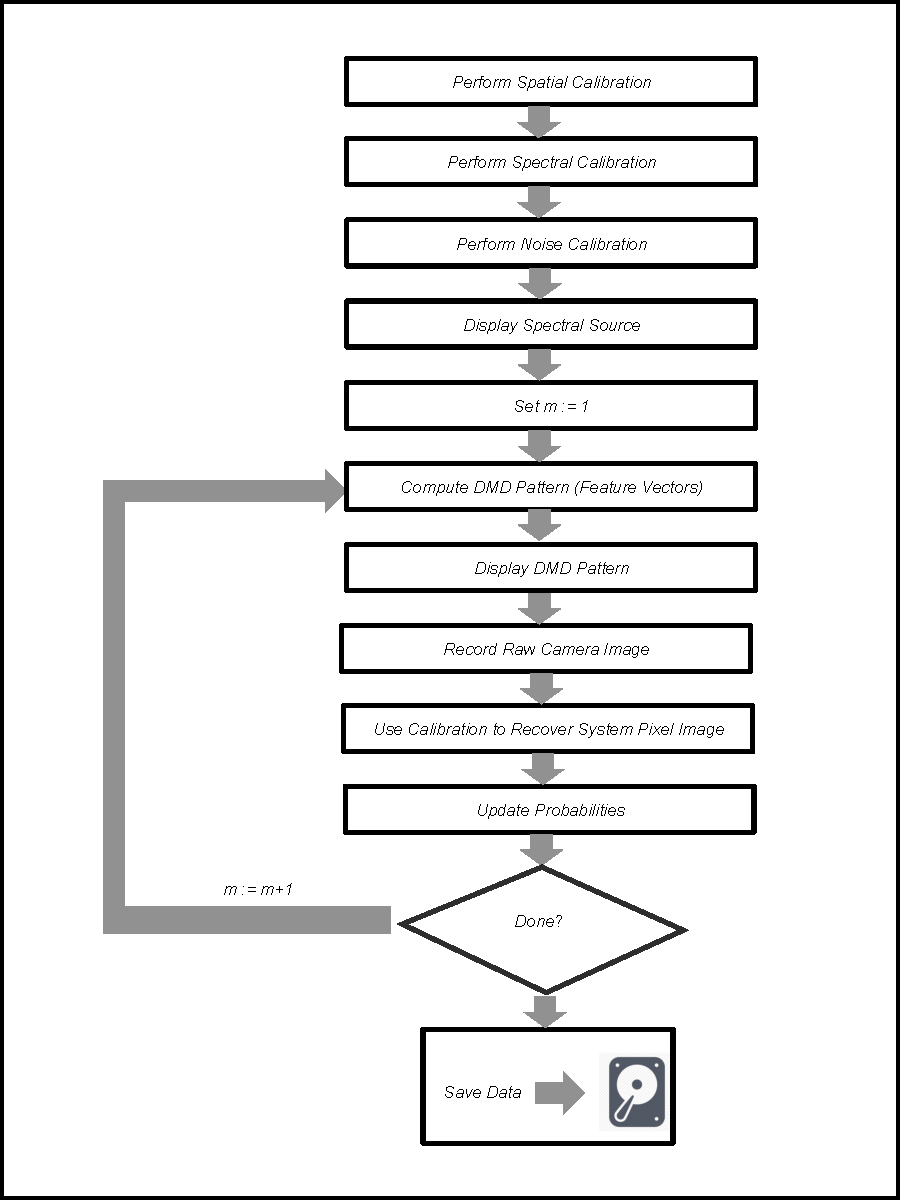
\includegraphics[scale=1.0]{afssicFlowchart}\\
	\captionof{figure}[Systems Level Flowchart for AFSSI-C Experiment]{Systems Level Flowchart of the AFSSI-C Experiment}
	\label{fig:afssicFlowchart}
\end{figure}


Classification difficulty is quantified as the \acrfull{tsnr} which considers the noise in the system relative to the separation distance between hypotheses spectra. We define \gls{tsnr} as
%
\begin{equation}
\text{TSNR} = 10 \log_{10} \ap{ \frac{d_{min}}{\sigma} }
\end{equation}
%
For our experiment, the noise is approximately \gls{awgn} distributed with standard deviation $\sigma$. The minimum Euclidean distance between the hypotheses in the spectral library $d_{min}$. When using this definition for TSNR, a value of 0 dB TSNR is the point where the noise is equal to the minimum distance between the library elements.


% Plot of the \gls{afssi-c} 4 Class Spectral Library
\begin{figure}[htb]
	\centering
	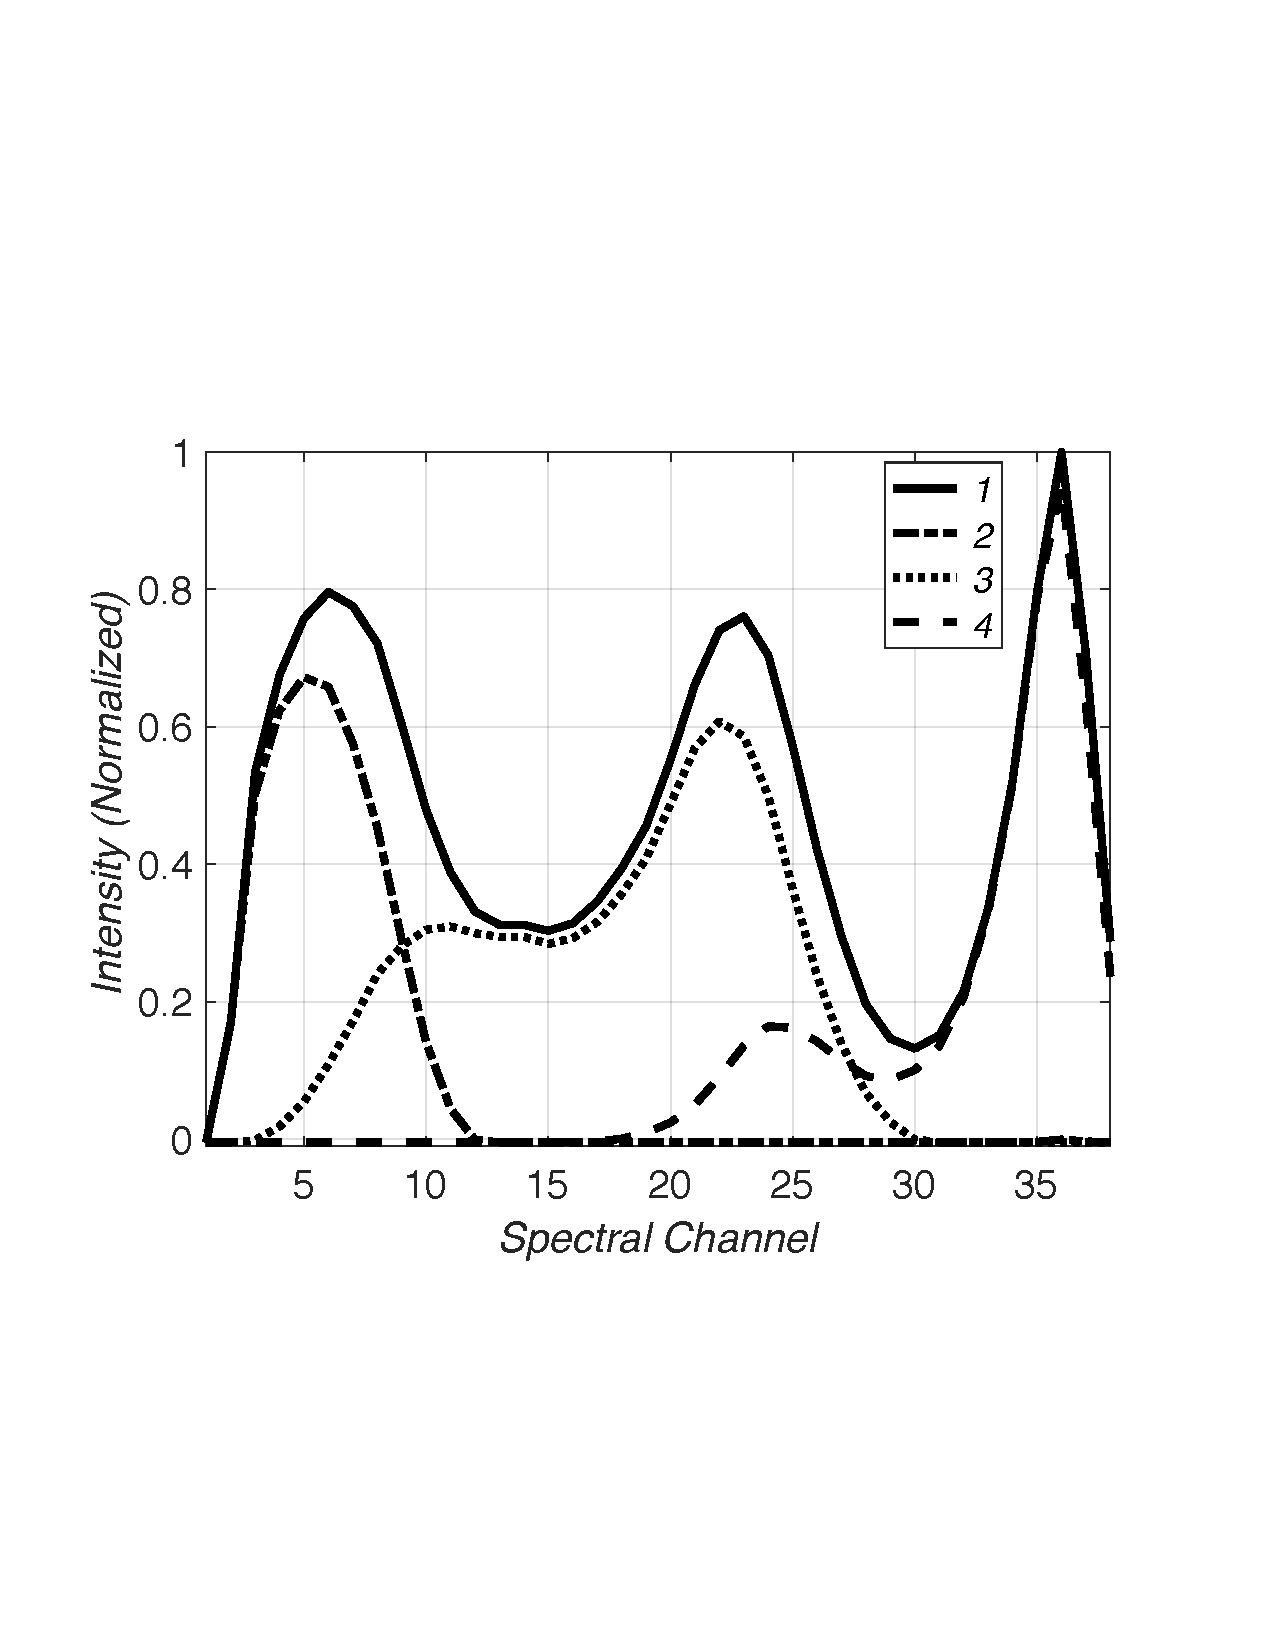
\includegraphics[scale=0.845]{afssicSpecLib}\\
	\captionof{figure}[Four class spectral library used for the AFSSI-C experiment.]{The spectral library consists of four spectral classes: the white, red, green, and blue of the LED monitor.}
	\label{fig:afssicSpecLib}
\end{figure}


% Plot of the UofA Symbol
\begin{figure}[htb]
	\centering
	
\includegraphics[scale=0.90]{afssicUofAsource}\\
	\captionof{figure}[Four class spectral source used for the \gls{afssi-c} experiment]{Four class spectral source used for the AFSSI-C experiment.}
	\label{fig:afssicUofAsource}
\end{figure}

\subsection{Hardware}

I will now discuss the hardware used in the \gls{afssi-c} experiment, shown in \Cref{fig:afssicPhoto1}. Specifically I will describe some of the design decisions and consequences of those decisions in the \gls{afssi-c} experiment. To avoid expensive and time consuming optical design and fabrication, the lenses were restricted to commercial off-the-shelf achromatic doublets. A compact, fixed focal length, lens (Edmund Optics Stock No. 58-001, f = 12mm) is used as an objective lens, relaying the object onto an intermediate image plane. A fast entrance optic is needed to meet the layout and magnification requirements. Referring to \Cref{fig:afssArch}, lenses 1 and 4 are 75 mm focal length achromatic doublets with a 50 mm diameter (Edmund Optics Stock No. 49-291), and lenses 2 and 3 are 150 mm focal length achromatic doublets with 25 mm diameter (Edmund Optics Stock No. 47-643). 

% joint-pPCA figure
\begin{figure}[htb]
	\centering
	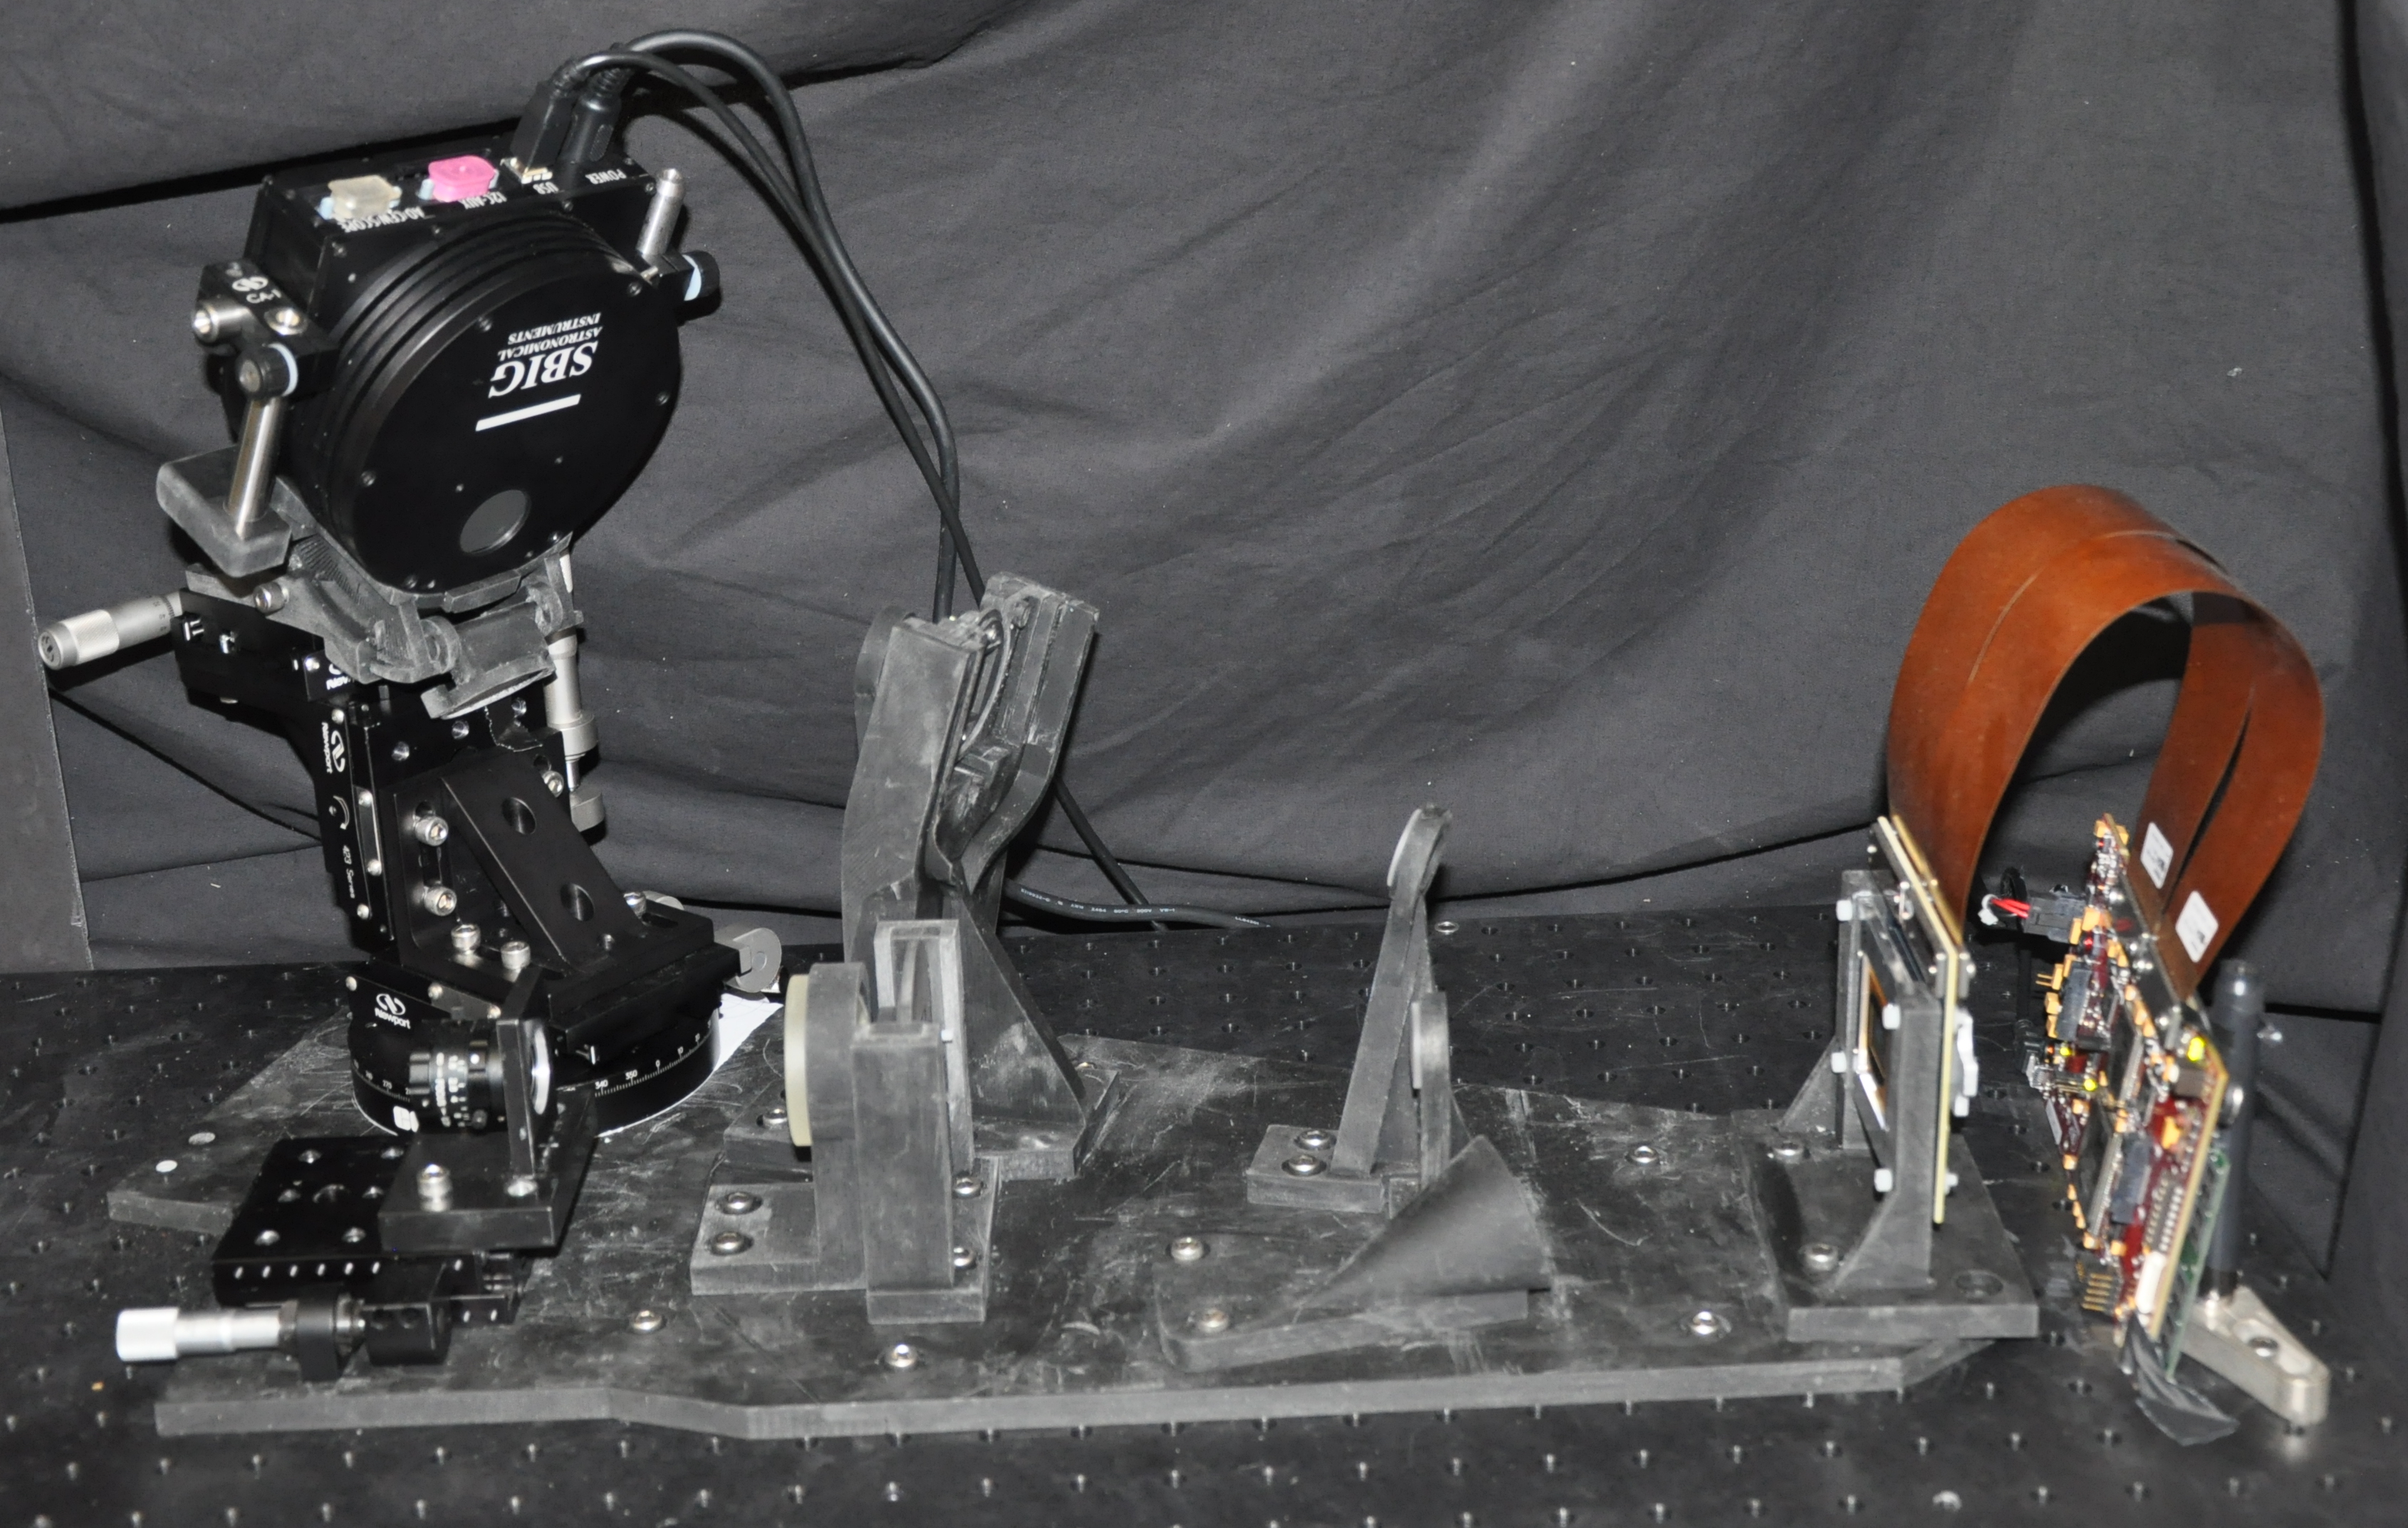
\includegraphics[height=3.7in]{afssicPhoto1.JPG}\\
	\captionof{figure}[Photograph of AFSSI-C.]{Photo of \gls{afssi-c}}
	\label{fig:afssicPhoto1}
\end{figure}

For a repeatable, programmable synthetic datacube source, we used an LED display (Dell P2311H LED monitor with 248 \textmu m pixel pitch). Though this limits the spectra we were able to generate, it still allows for programmable spectra at every spatial location. The center 1080 $\times$ 1080 pixels are used to generate the source spectral datacubes. Spectra consist of combinations of the RGB monitor colors.

The \gls{afssi-c} operated at a spectral range of 425-625 nm, which is approximately the visible wavelength range. We placed thin-film spectral filters in the collimated space to attenuate light outside of this range. The system is designed for $N_{\lambda} = 38$ spectral channels, resulting in roughly $5$ nm/spectral channel. The system magnification to the \gls{dmd}, which then dictates the lateral spread allowed per spectral channel, requires custom 0.10 lines \textmu m holographic blaze gratings as the dispersive elements, fabricated by Wasatch Photonics. The gratings are designed to minimize diffraction in all the orders except the first order. 

The \gls{dmd} used in our experimental prototype was manufactured by Texas Instruments, it is a DLP Discovery 4100 \gls{dmd} development kit, with the DLP9500 0.95" 1080p \gls{dmd} chipset. The \gls{dmd} has 1080 $\times$ 1920 10.8 \textmu m mirrors on the array, and the mirrors pivot 12 degrees on a diagonal axis. The \gls{dmd} is oriented such that the bottom of the array is parallel to the optical table, which forces the second arm of the \gls{afssi-c} to rise off the optical table at an angle of 17.5 degrees; this orientation was chosen so that the mirrors would be oriented as squares rather than diamonds. While the periodic structure of the \gls{dmd} can produce strong diffraction for certain types of illumination, no diffraction effects are observed in the \gls{afssi-c} as the light incident on the \gls{dmd} is incoherent. 

A Santa Barbara Instrument Group (SBIG) ST-10XME detector with a 2184 $\times$ 1472, 6.8  \textmu m pitch \gls{ccd} as the camera. Due to the angle of the optical axis of the second arm of the \gls{afssi-c}, a goniometer was constructed using a rapid prototyping 3D printer to facilitate easy alignment of the SBIG camera \cite{dunlop-gray2015phdthesis}.

%ecause we are interested in a quantitative system analysis, we compare measurements on the discretized detector to what was projected by our discretized source. The layout dimensions, component pixel size, and lens design were tuned to yield pixel groups---referred to here as \gls{sp}s---at each component that are an integer number of the component pixel, or in the case of the \gls{dmd}, integer number of mirrors. We therefore have the following \gls{sp} dimensions: $16 \times 16$ pixels on the source, $8 \times 8$ \gls{dmd} mirrors, and $12 \times 12$ pixels at the detector.

Once the optical layout was finalized, the physical system was designed in SolidWorks. The lens mounts, detector mount, \gls{dmd} mount, beam dump, and locating plates were then fabricated on a Eden 350 rapid prototyping 3D printer.

Light baffling is utilized to shield the system from ambient light as well as stray light within the system. A baffling structure was designed and printed to surround the detector, with smaller baffling elements to attenuate stray light around the optical paths.


\subsection{Implementing Codes}

One of the practical considerations of the coding scheme in the \gls{afssi-c} is that the pPCA algorithm generates both positive and negative elements in the feature vectors. These are analogous to having positive and negative weights in the weighing problem. Unfortunately, with incoherent light, one is unable to make simultaneous positive and negative measurements because we cannot easily manipulate the phase of the electric field. Therefore, in the \gls{afssi-c} we are forced to take two camera exposures for each measurement step and subtract the negative set of measurements from the positive set of measurements. This means that an additional noise term is added to each measurement step. For the rest of this chapter, when I say measurement or measurement step, I really mean one  measurement step which records two camera exposures.

Another practical issue is that the \gls{dmd} we used only allows a binary mode of operation. Either the mirror reflected the light towards the second arm or it reflected light towards the beam dump. In practice any positive element is set to $1$ and any negative element is set to $-1$. 

\subsection{Calibration}

One reoccurring topic in this dissertation is calibration. In computational sensing the measurement may not look anything like the signal-of-interest. Just like in the \acrfull{scout}, the \gls{afssi-c} relies heavily on several calibration procedures which involves spatial, spectral, and noise measurements for optimal classification performance.


\subsubsection{Spatial Calibration}

One of the major opto-mechanical issues in the \gls{afssi-c} is caused by the geometry of the \gls{dmd} with respect to the second arm. The \gls{dmd} plane is normal to the optical axis of the first arm, but it is at an angle (equal to twice the tilt of the mirrors on the diagonal) to the second arm. One can think of the \gls{dmd} plane as the object plane for the second arm of the system. Since the \gls{dmd} is tilted, this creates an Scheimpflug distortion: a tilted object plane images to tilted image plane \cite{smith1966modern}. 

Because of Scheimpflug distortion, the image of the monitor physical pixels are not aligned to the rectangular grid of pixels on the \gls{fpa}, see \Cref{fig:rawDetReadoutOfUofALogo}. Even worse there is not a one-to-one relationship of \gls{fpa} pixels to object scene pixels since the magnification is not constant over the \gls{fov}.  In order to produce optimal performance we need to know the mapping of monitor to \gls{fpa} pixel locations. The goal of spatial calibration is to make a set of measurements in which we can infer a parameterized relationship from \gls{fpa} physical pixel coordinates to monitor physical pixel coordinates. 


\begin{figure}[htb]
	\centering
	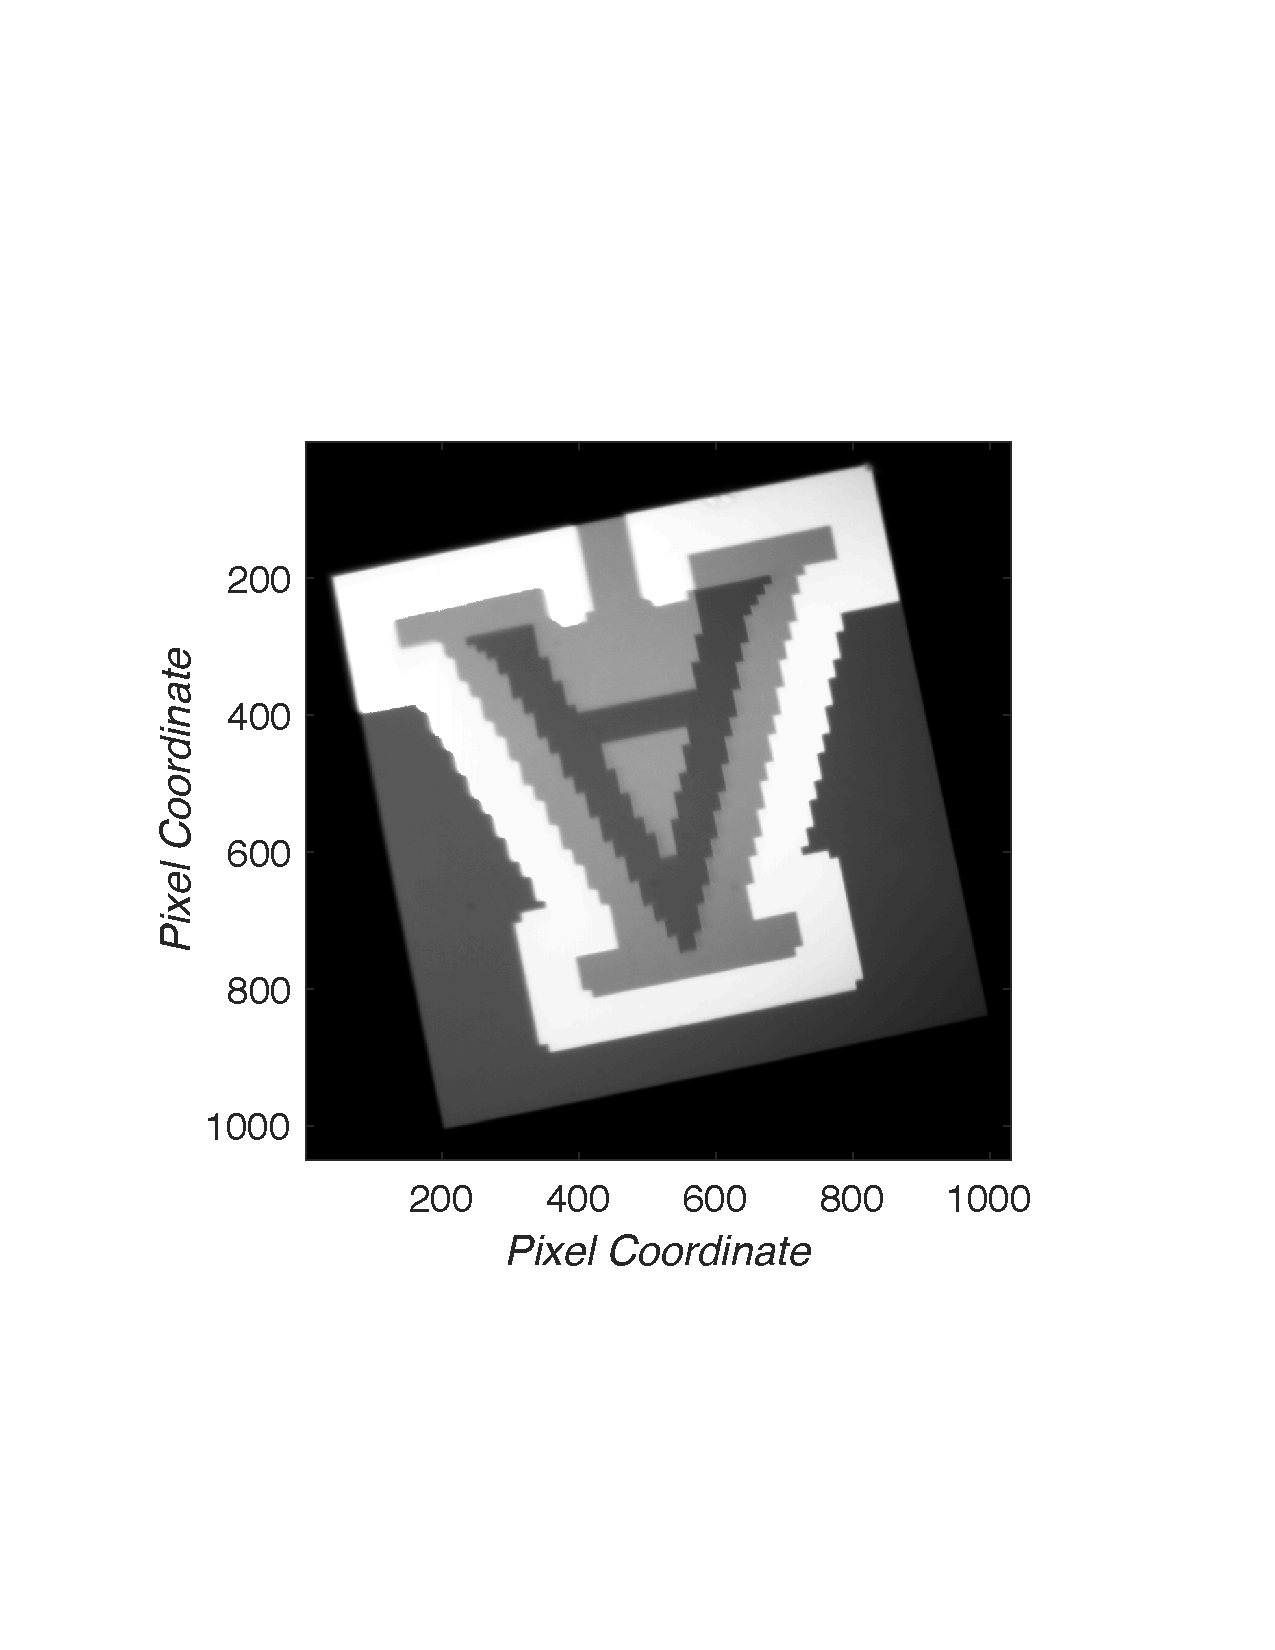
\includegraphics[scale=0.75]{rawDetReadoutOfUofALogo}\\
	\captionof{figure}[The image produced by the camera without any post-processing.]{The image produced by the camera without any post-processing.}
	\label{fig:rawDetReadoutOfUofALogo}
\end{figure}


Due to spatial resolution constraints and other practical issues, we grouped several physical pixels together in a \acrfull{sp}. For example, in our experiment we have an effective resolution of 64 $\times$ 64 \gls{sp}s. However, on the monitor a \gls{sp} actually consists of 16 $\times$ 16 physical pixels on the source. Similarly, on the \gls{dmd} a \gls{sp} consists of 8 $\times$ 8 physical pixels (mirrors) and on the detector a \gls{sp} consists of 12 $\times$ 12 physical pixels.


A straightforward approach to inferring the relationship between \gls{fpa} and object scene pixels would be to energize each physical pixel on the \gls{roi} one at a time and record the image on at the physical pixel. We could then create a look-up table for each \gls{fpa} pixel to infer where from the LED this came from. However, energizing each of the 1024 $\times$ 1024 physical pixels at 5 seconds per exposure will take approximately 61 days. We are therefore forced to infer the spatial transform from a small number of physical pixels images.

At this point we are only concerned with how the the LED monitors appear on the \gls{fpa} image. The alignment of the \gls{dmd} does affect the image quality and location, but the pattern of the \gls{dmd} only affects the radiance of an image point. Therefore, we set the entire \gls{dmd} mirror pattern to reflect towards the second arm. In this state, the \gls{dmd} acts like a normal mirror. 

First the monitor displays a grid of white dots, \Cref{fig:gridOfWhiteDotsForSpatialCalibration1}. The number of dots can be then be increased for better accuracy but increases the calibration time. The list of monitor physical pixel coordinates where the center of each dot appeared on the monitor is then saved.

\begin{figure}[htb]
	\centering
	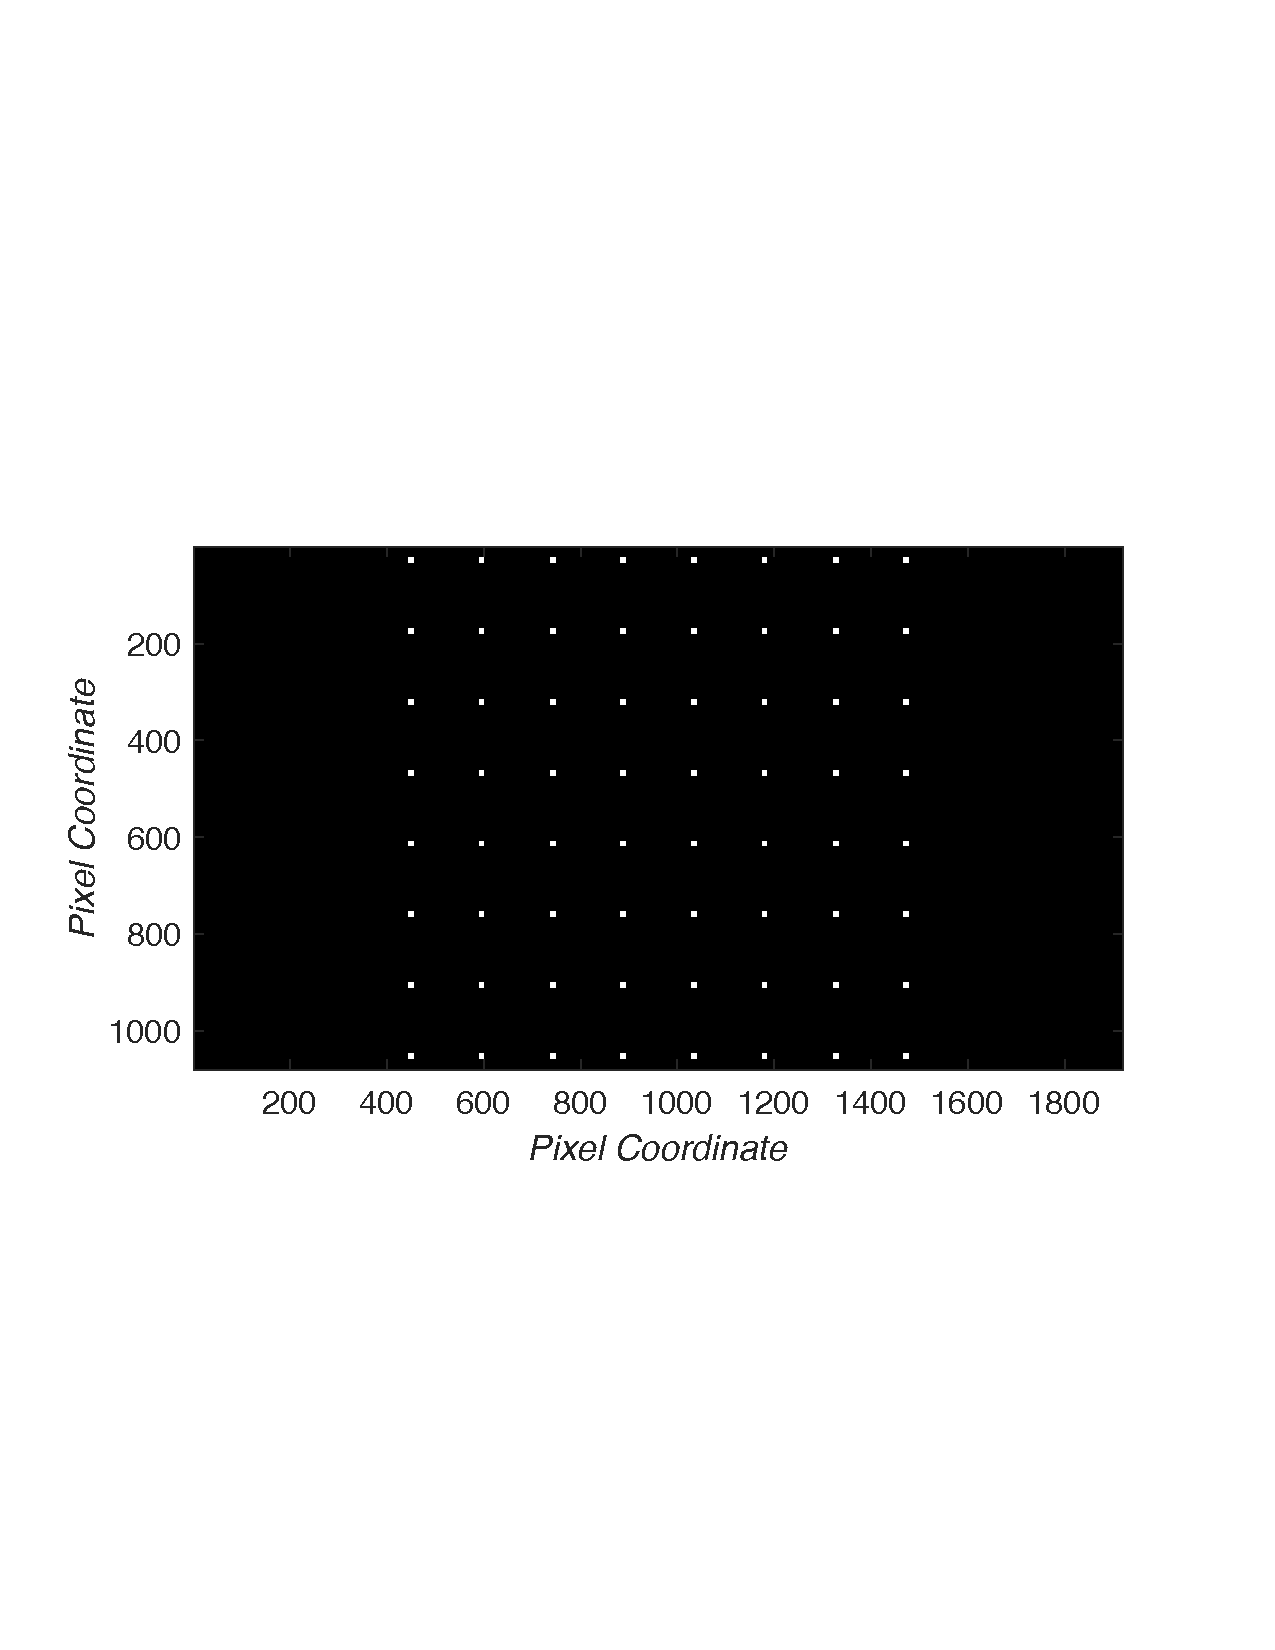
\includegraphics[scale=0.81]{gridOfWhiteDotsForSpatialCalibration1}\\
	\captionof{figure}[Spatial Calibration Grid of Dots Used In \gls{afssi-c} Experiment]{An array of white dots is displayed on the monitor as part of the spatial calibration. The image of this grid is recorded, the centroids are estimated and a spatial transform is inferred between the physical pixel coordinates of the LED monitor and the \gls{fpa}}
	\label{fig:gridOfWhiteDotsForSpatialCalibration1}
\end{figure}

A raw camera image is captured and stored, see \Cref{fig:detReadOutOfDots}. To account for hot pixels and systematic error in the system the camera image of the all black monitor is subtracted from the camera image of the array of white dots which gives us the dark subtracted image of white dots. The dark subtracted detector image is then thresholded to prevent noisey pixels from being counted as one of the images of the white dots from the monitor. All values above the threshold is set to 1 while all values below the threshold is set to 0.

Using a built-in MATLAB \texttt{regionprops} function with the optional \texttt{centroid} argument, we can infer the center pixel, centriod, for each of the white dot images in the thresholded image. This function generates a list of pixel coordinates from the thresholded image. Each pixel coordinate is associated with the center of each white dot in the image. Often times however, we get a list of coordinates is that more or less than the number of white dots displayed onto the monitor. At this point, we may need to change the threshold value to return the same number of coordinate pairs as dots displayed on the monitor. For example if we have an 8 $\times$ 8 grid of dots we expect a list of 64 detector pixel coordinate pairs. As a sanity check, we can create an image of the where the inferred centriods are and overlay it on thresholded image of the grid of white dots. The image of the centriods should be approximately on top of the image of each white dot, see \Cref{fig:centriodsOverlayedOnTheThresholdedImage}.

\begin{figure}[h]
\includegraphics[scale=0.7]{detReadOutOfDots}
\centering
\caption{The detector image of the array of white dots as part of the spatial calibration}
\label{fig:detReadOutOfDots}
\end{figure}

\begin{figure}[h]
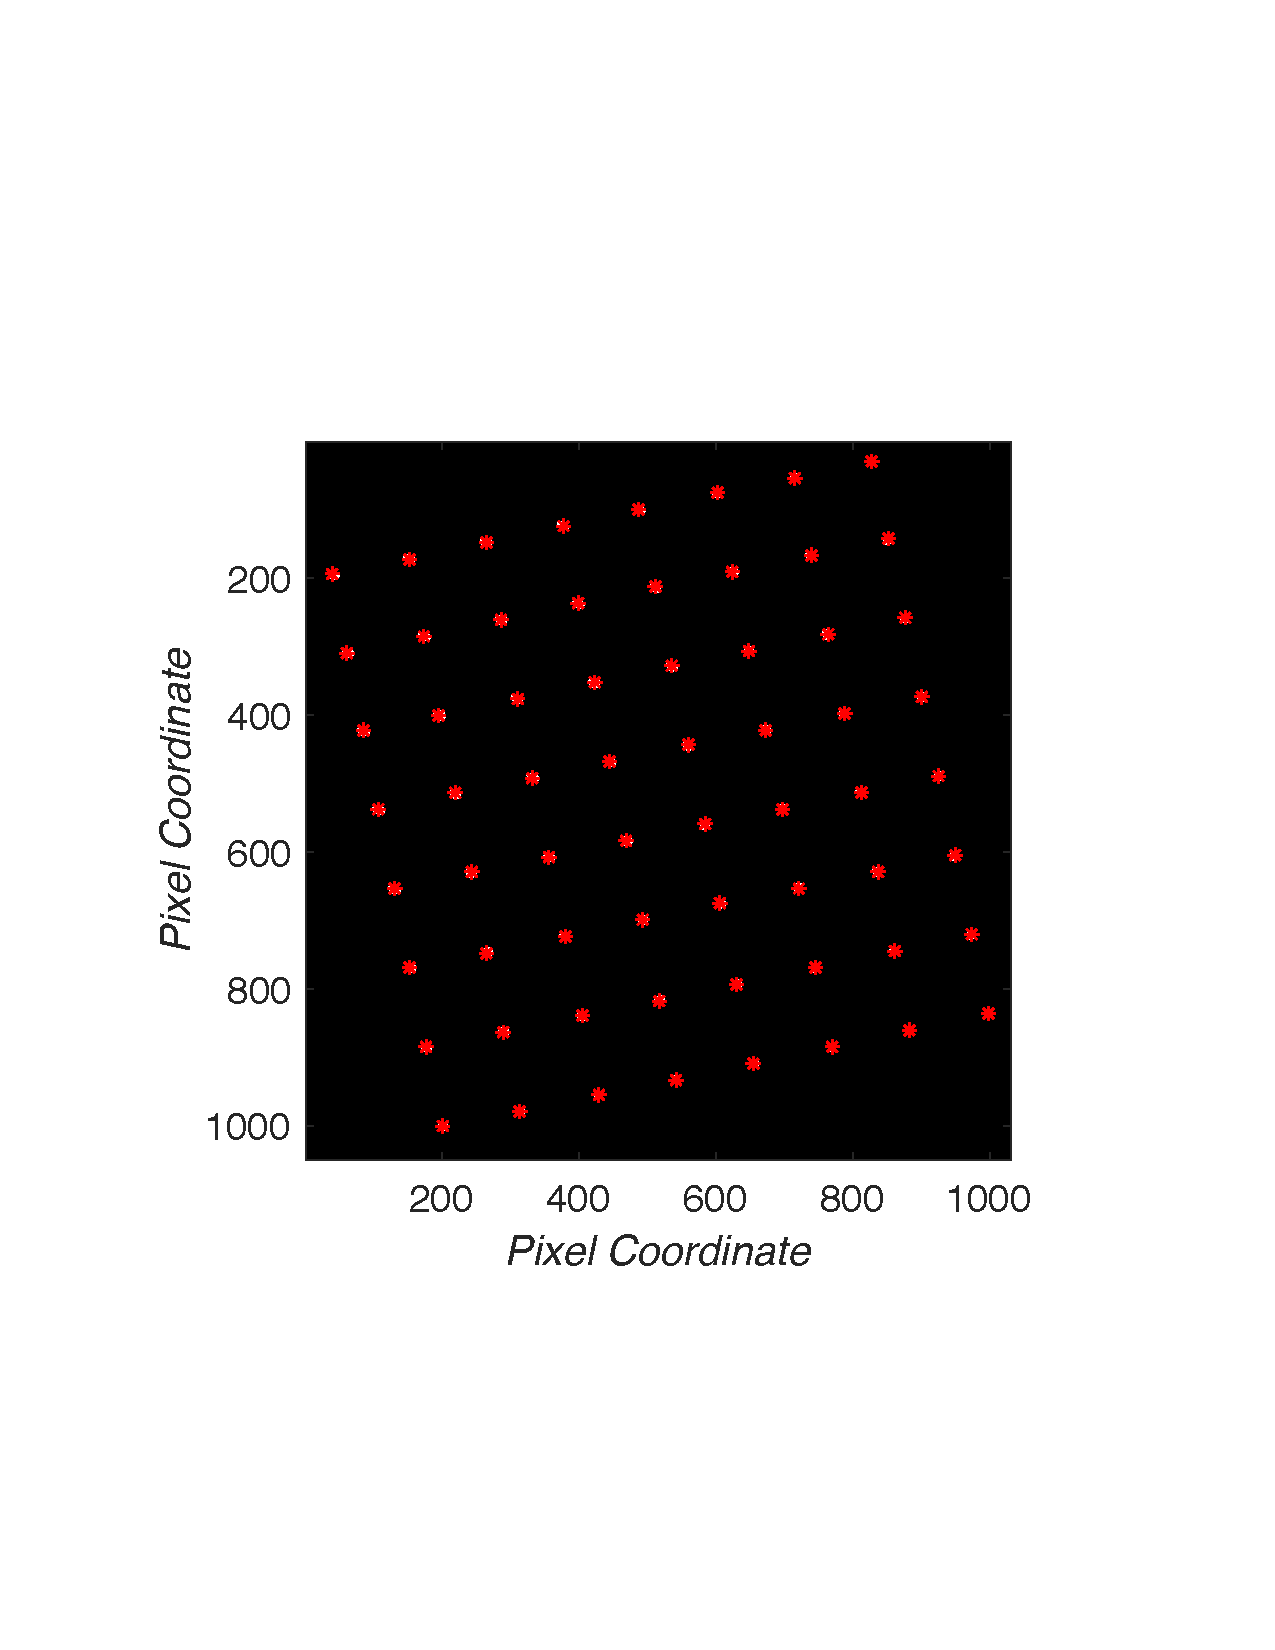
\includegraphics[scale=0.7]{centriodsOverlayedOnTheThresholdedImage}
\centering
\caption{The detector image of the array of white dots as part of the spatial calibration}
\label{fig:centriodsOverlayedOnTheThresholdedImage}
\end{figure}

Each dot is added to the monitor scene one at a time to prevent accidently associating the wrong dot on the image. Doing this each time the \gls{afssi-c} is calibrated is time consuming, since we need at least as many \gls{fpa} exposures as there are dots in the object scene. In practice, we use MATLAB to look up the locations from the last spatial calibration and if we believe the instrument has not been misaligned since then, we look in a neighborhood of pixels around the last dot locations and compute the centroids of the dots, see \Cref{fig:theFinalSquareLocatesTheFinalDot}.


\begin{figure}[h]
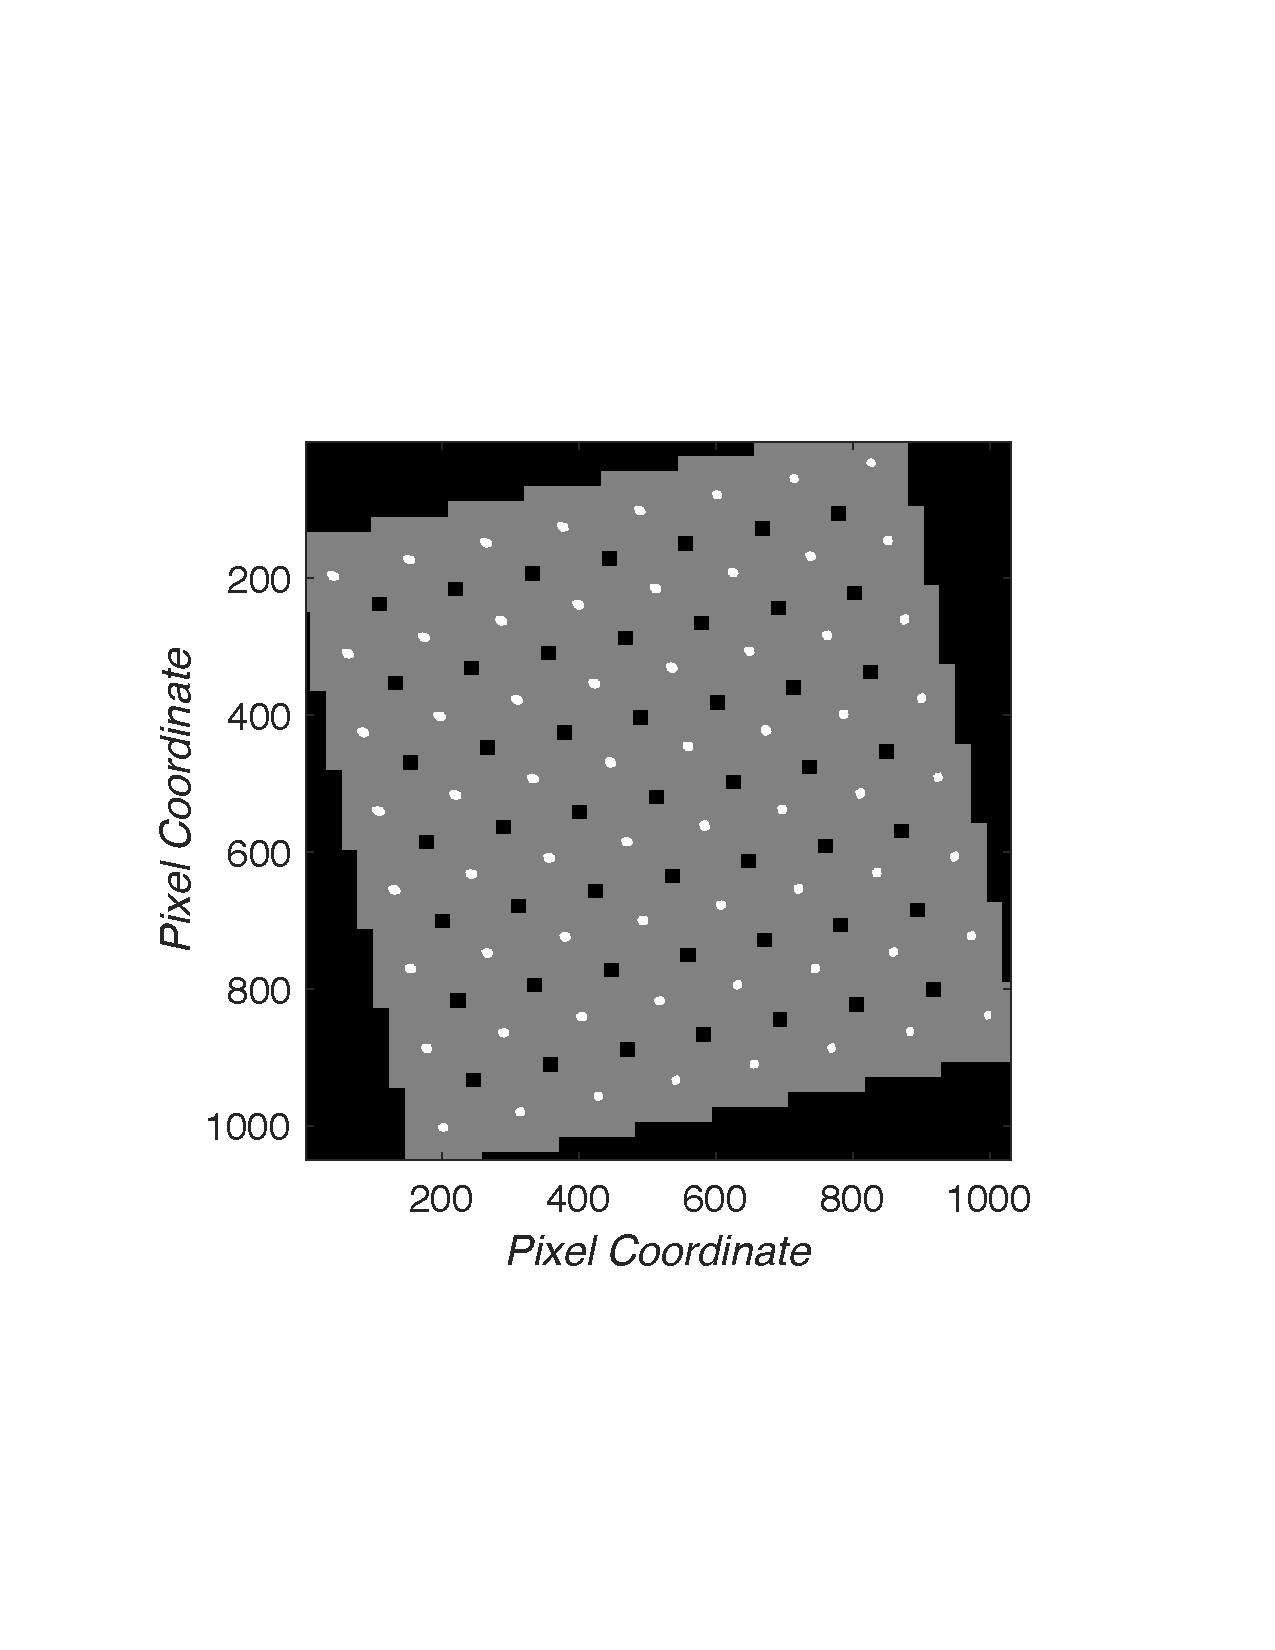
\includegraphics[scale=0.7]{theFinalSquareLocatesTheFinalDot}
\centering
\captionof{figure}[Speeding Up Spatial Calibration By Looking In Regions Around Previous Spatial Calibration Image Dots]{Instead of displaying the dots one at a time, we use the location of the dot images from the last spatial calibration and search in a rectangular region around those coordinates for the new dots. This greatly speeds up the spatial calibration since each exposure is approximately 3-5 seconds.}
\label{fig:theFinalSquareLocatesTheFinalDot}
\end{figure}


Now that we have a list of dot centers in the monitor pixel coordinates and a list of dot centers in the detector pixel coordinates, we use the MATLAB function \texttt{cp2tform}, which takes the list of control points and uses them to infer the spatial transform. This transform is a parameterized relationship between every single physical pixel coordinate on the monitor and physical pixel coordinate on the detector. 

Each \gls{sp} contains $16 \times 16$ physical pixels, using the spatial transform, we known which detector pixels these physical pixels will image to. The average value of all the physical pixels from the \gls{fpa} image correspond to the \gls{sp} value. Thus we can reverse the effects for any image rotation or translation at the \gls{fpa} plane.

As part of the calibration procedure, an image is saved by turning on the entire DMD and measuring the intensity at each spatial location with the monitor set to white at full intensity. One can think of this image as an intensity map, providing information as to which locations have more throughput than others in the \gls{fov}. During the classification operation, each camera image is normalized by this intensity map, while the spectral library at each location is normalized by the integration of the white spectrum (which has the system spectral response information folded into it), allowing the classification decisions to be made. 


\subsubsection{Spectral Calibration}

Unfortunately, due to vignetting and imperfections in the gratings the spectral response of the \gls{afssi-c}, the combined optical system produces a shift-invariant spectral response. To correct for this we developed a calibration procedure to measure how the spectral response of the optical system varies over the region-of-interest in the \gls{fov}. 

A flowchart of the spectral calibration is shown in \Cref{fig:grabRawDetectorImagesForResponseCubes}. Remember that in the \gls{afssi-c} architecture, the first column of mirrors on the \gls{dmd} reflects light corresponding to the first spectral channel of the first spatial column. The second column of mirrors reflects light corresponding to the first spectral channel of the second spatial column and also reflects the light in spectral channel 2 of the first spatial column, and so on, see \Cref{fig:fastSpectralCalibration}. Also, the dual-disperser architecture of the \gls{afssi-c} means that light from a single spatial pixel images to a single spatial pixel on the \gls{fpa}, regardless on what pattern is being displayed on the \gls{dmd}. In other words, in a single camera image image we can measure the intensity of different spectral channels of adjacent spatial locations along a row by turning on only one \gls{dmd} mirror. Therefore, we can turn on an entire row of pixels in the monitor and realize that different \gls{fpa} images correspond to different spectral channels for each spatial location. 

Also remember that the dispersion is only in the horizontal direction, along the columns of the \gls{dmd}. Therefore, we can set the entire \gls{roi} to display the same spectrum. Then sweep the entire column of the \gls{dmd}. In our experiment, the number of effective \gls{dmd} \gls{sp} columns is equal to the number of monitor \gls{sp} in a row plus the number of spectral channels minus one 
%
\begin{equation}
	N_{d_x} = R_x + N_{\lambda} - 1
\end{equation}
%
Therefore, we had 101 \gls{dmd} \gls{sp} columns. So the first 38 camera images corresponds to the 38 spectral channels in the first spatial \gls{sp} column. Then images 2 to 39 correspond to the first 38 spectral channels in the second spatial \gls{sp} column. 

Another way to reduce the spectral calibration time is by realizing that we can turn on two \gls{dmd} \gls{sp} columns at a time. This is because we only have 38 spectral channels and 101 DMD \gls{sp} columns. So in our calibraiton procedure we turn on two \gls{dmd} \gls{sp} columns at a time each 50 \gls{sp} columns apart. Then for each spectrum in spectral library we only need 51 exposures. If we assume a 5 second expsoure this only takes about 20 minutes. In practice we use a much longer exposure time to increase the \gls{snr} of each \gls{fpa} exposure. The total time for a four class spectral library is approximately 4 hours.


\begin{figure}[h]
	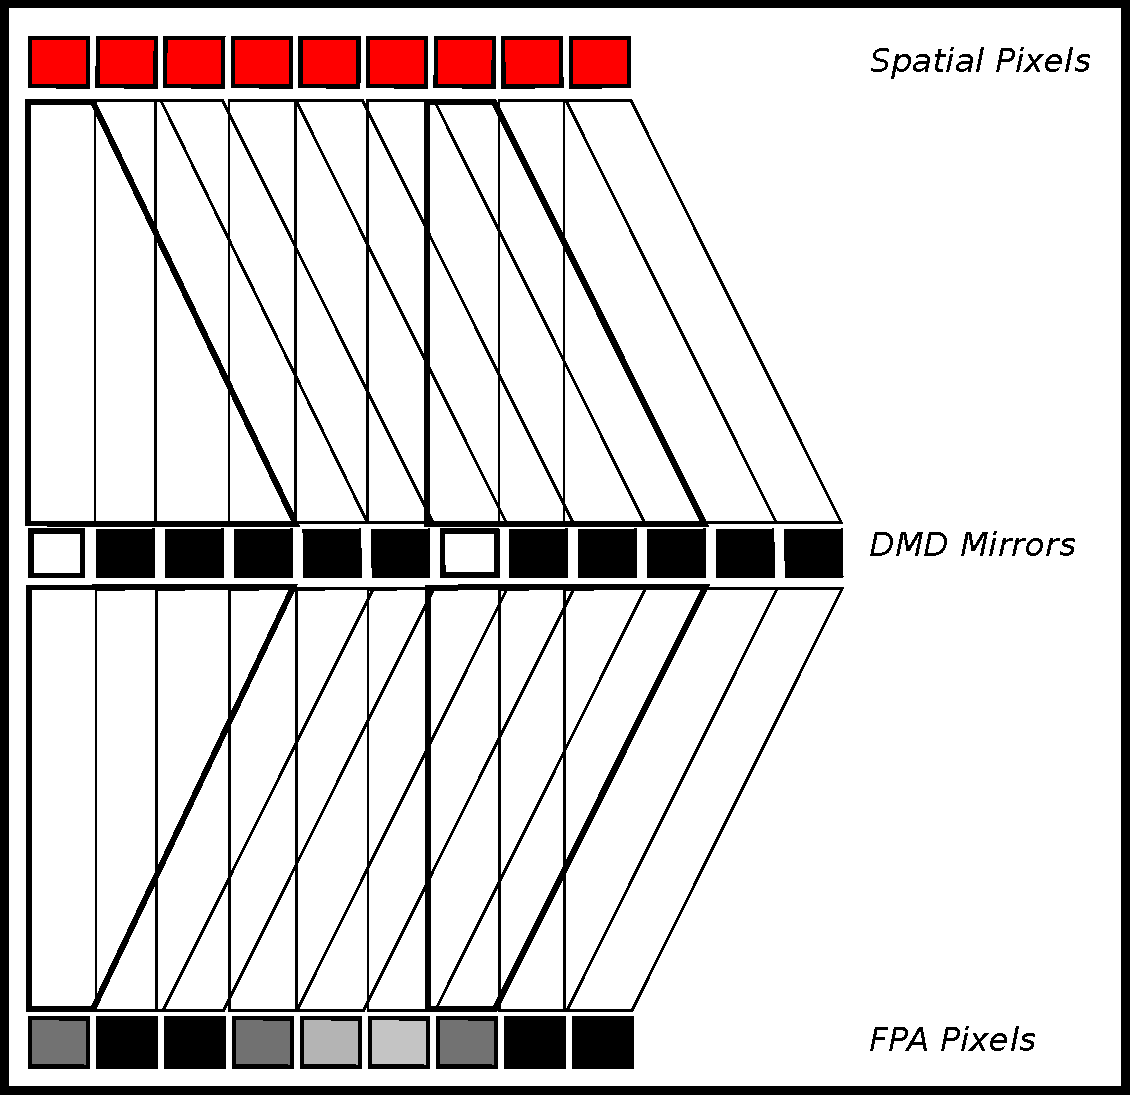
\includegraphics[scale=0.7]{fastSpectralCalibration}
	\centering
	\captionof{figure}[Depiction of spectral calibration]{In order to speed up the spectral calibration we turn the entire monitor ROI to the same spectrum and sweep two DMD columns at a time.}
	\label{fig:fastSpectralCalibration}
\end{figure}

\clearpage
	\begin{figure}[H]
	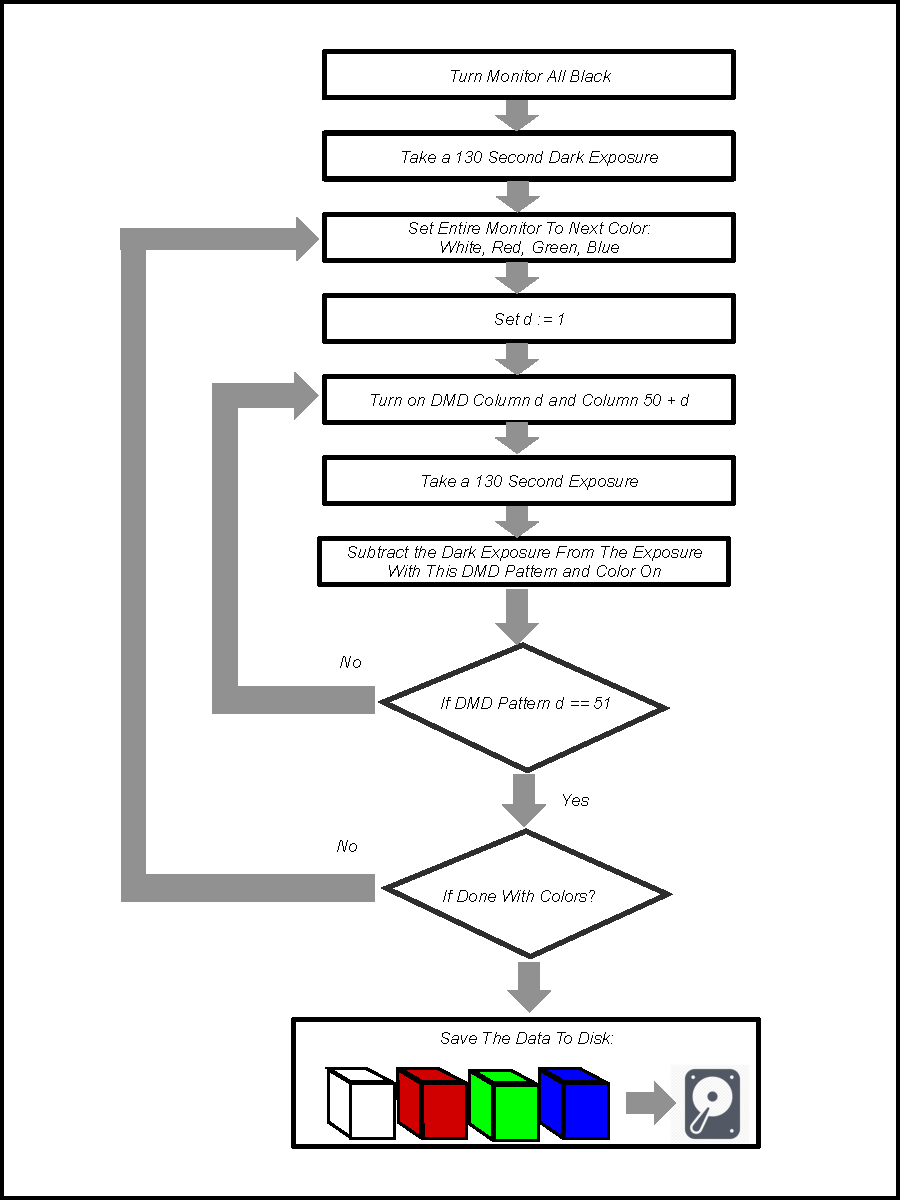
\includegraphics[scale=1.0]{grabRawDetectorImagesForResponseCubes}
	\centering
	\captionof{figure}[Depiction of spectral calibration]{In order to speed up the spectral calibration we turn the entire monitor ROI to the same spectrum and sweet two DMD columns at a time.}
	\label{fig:grabRawDetectorImagesForResponseCubes}
\end{figure}


\subsubsection{Noise Model Calibration}

As I discussed in \Cref{ssec:updatingProbabilities}, the adaptive algorithm we used to make classification decisions compares the ratio of posterior probabilities by updating ratios of the likelihoods after each measurement. The likelihood is defined as the probability of the measurement given that the hypothesis is true. This probability is given by the noise model using \Cref{eq:noiseModel1}. Accurate estimation of the noise standard deviation, $\hat{\sigma}$, is required for optimal classification rates. 

If $\hat{\sigma}$ is much larger than the actual value,  $\sigma$, then the probability for different spectral classes will tend to be similar. However, as I discussed, the \gls{ppca} algorithm depends on weighting the probability of some classes higher than others to outperform non-adaptive systems. This may lead to longer convergence times to the correct class. If the $\sigma$ is too small then the algorithm may converge to the wrong class. 

Fortunately estimating the noise of the system is a relatively straightforward. At each spatial \gls{sp} location we randomly choose one the spectra from the spectral library and display it, then the we display a random pattern on the entire \gls{dmd} record the camera image and compare the measured intensity value at each spatial location to what we expected from the simulated camera image. This is repeated several times until we have sufficient statistics to plot the distribution of the differences between measured and expected intensities, see \Cref{fig:noiseCalFit}. Using the MATLAB \texttt{fit} function with the one-dimensional Gaussian option \texttt{gauss1},we fit a Gaussian to the data to estimate the standard deviation of the noise, $\hat{\sigma}$.

The value of $\sigma$ is the intrinsic amount of noise in the instrument. It takes into account all possible sources of noise in the \gls{afssi-c}. However, we would like to vary the total amount of noise to see how the experimental classification performs compared to simulation and how the it performs compared to various other imaging spectrometers. This is done in post-processing by adding normally distributed noise with standard deviation $\sigma_{added}$ to the measurements. Since the intrinsic system noise is approximately Gaussian, the total variance is thus

\begin{equation}
	\sigma_{total}^2 = \sigma^2 + \sigma_{added}^2
\end{equation}

\begin{figure}[h]
	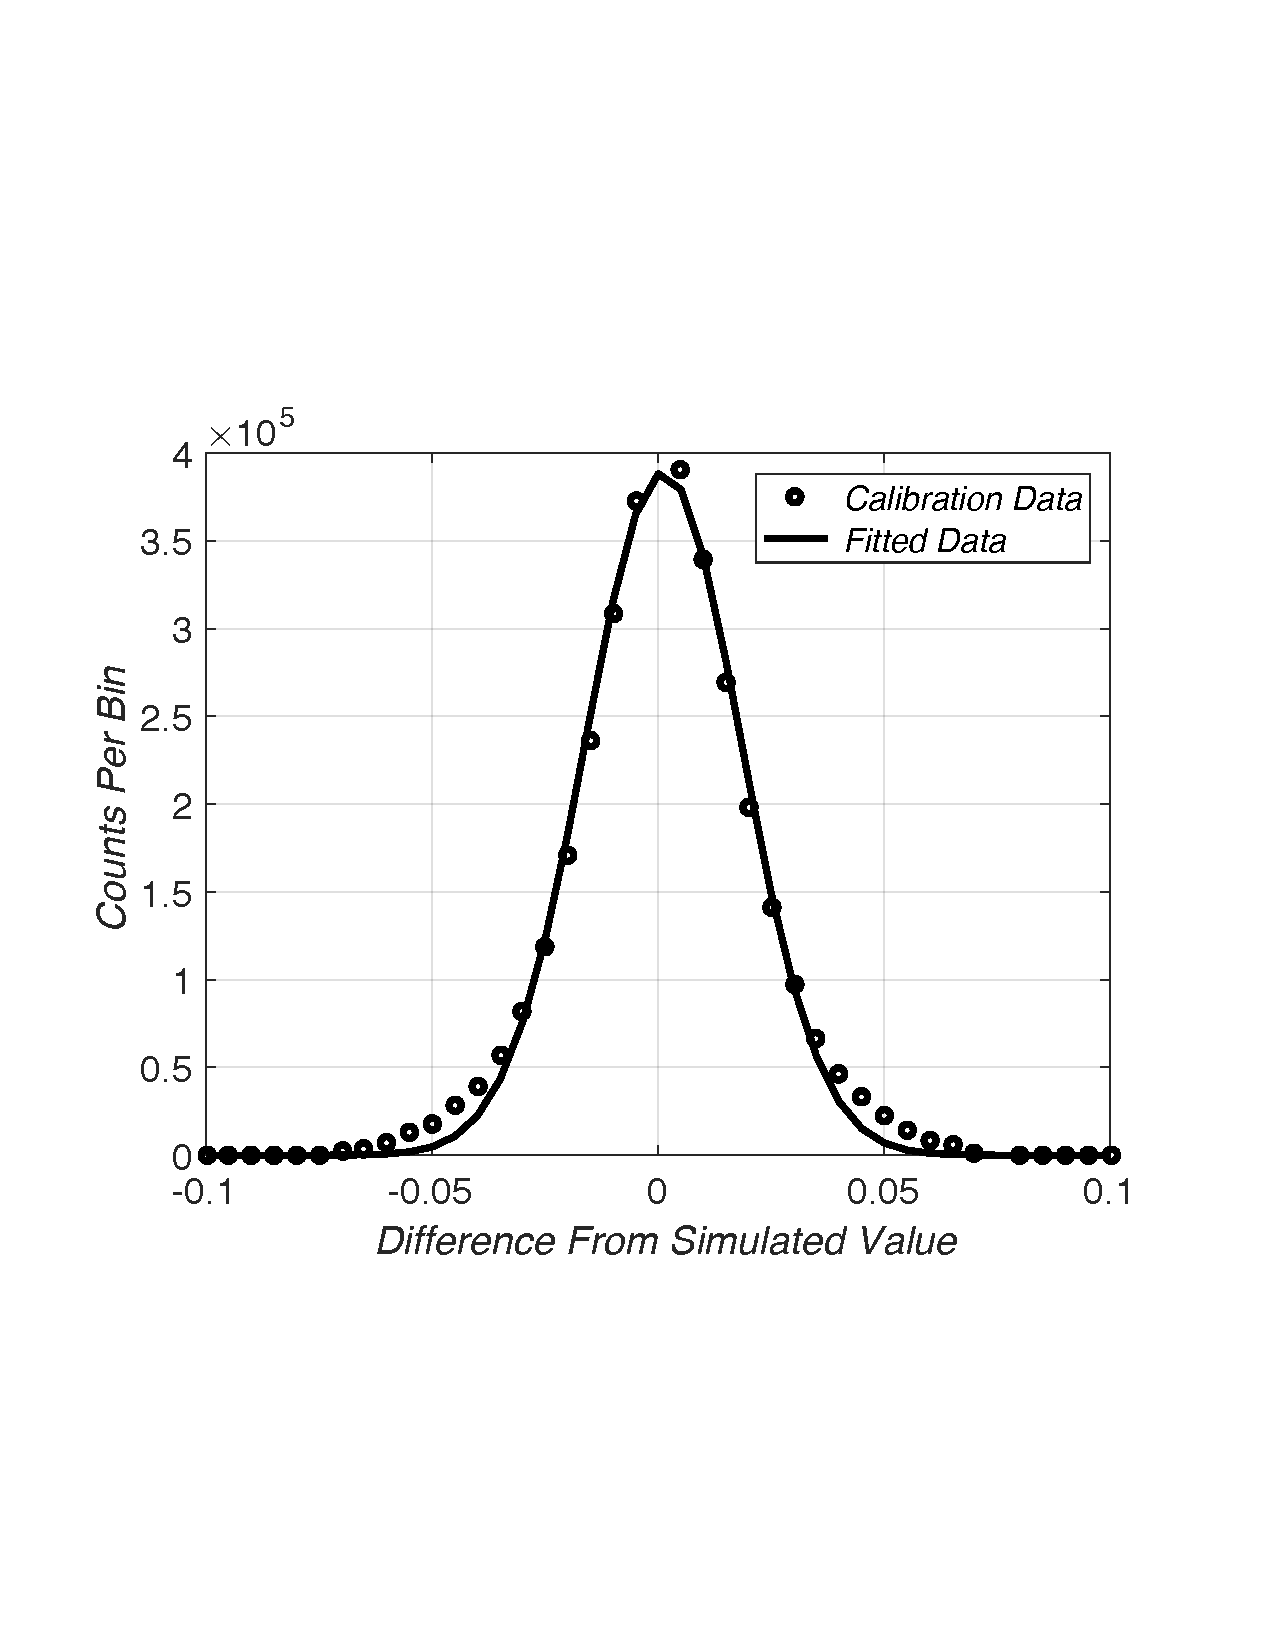
\includegraphics[scale=0.8]{noiseCalFit}
	\centering
	\captionof{figure}[Estimating the System Noise]{Estimating the System Noise: The circles represent the distribution of difference between the measurement and expected values of randomly chosen spectra with random spectral filters. The solid line represents a Gaussian fit, which allows us to estimate the standard deviation of the system noise.}
	\label{fig:noiseCalFit}
\end{figure}

\section{Experimental Results}


\Cref{fig:afssicExpResults3InChap} presents experimental classification results at 0, -3, and -6 dB TSNR after measurements. Measurements 1 through 30 are presented in Appendix \ref{app:afssicExpResults}. As the classification difficulty increases (lower TSNR), the adaptive algorithm takes more measurement steps to correctly classify. 

 \begin{figure}[htb]
  \centering
  % Requires \usepackage{graphicx}
  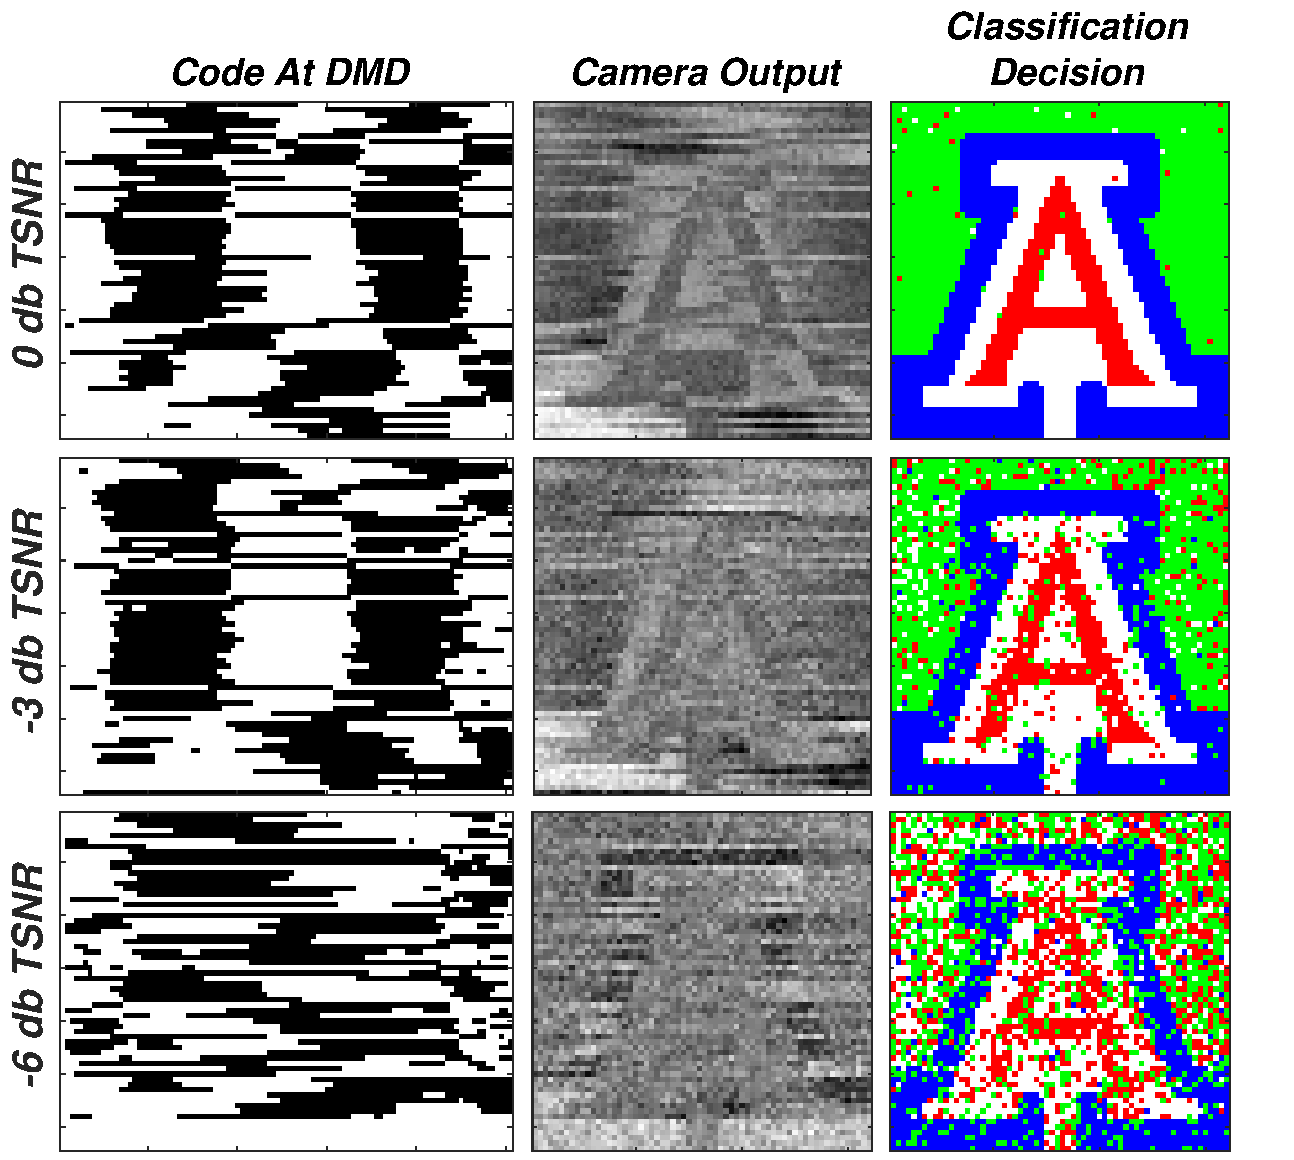
\includegraphics[scale=0.72]{afssicExpResults3}\\
  \caption{Data from after the third measurement step at 0, -3, and -6 dB TSNR. The left column is a depiction of the \gls{dmd} code, center is the output from the detector, and the right is the classification decision at the current measurement.}\label{fig:afssicExpResults3InChap}
\end{figure}

The experimental classification rates that we obtained agree well with simulation. \Cref{fig:SIMmultiTSNR} shows the performance of the \gls{afssi-c} experimental results and the simulated values. The simulated and experimental data are the average of 30 simulations and 10 experiments, for each of the four \gls{tsnr} values representing several levels of increasing classification difficulty (0, -3, -6, and -9dB TSNR).
%
%Experimental data with simulation
\begin{figure}[htb]
 	\centering
  	% Requires \usepackage{graphicx}
  	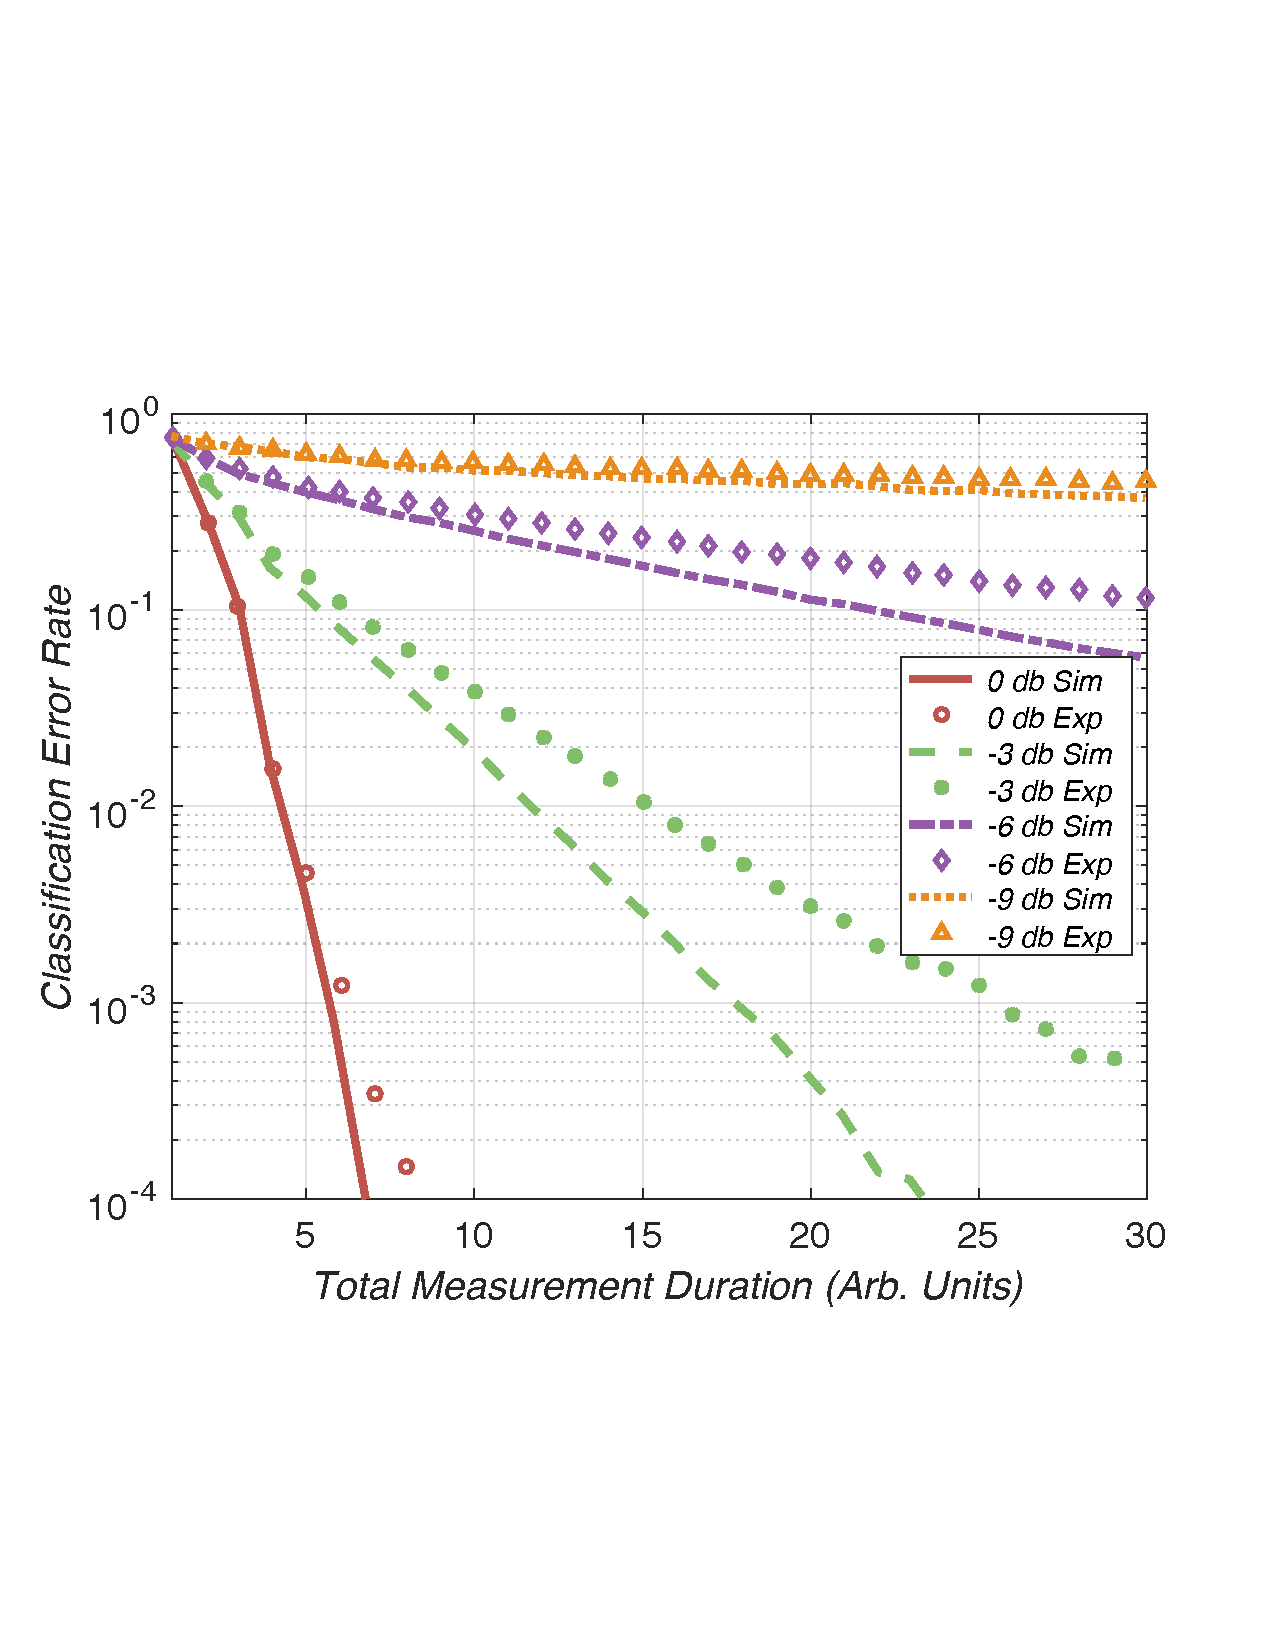
\includegraphics[scale=0.76]{afssicExpVsSim}\\
  	\caption{Comparison of the AFSSI-C experimental system results to the simulation results for multiple TSNR levels by plotting the classification error versus measurement. Shown are repeated experiments of a $64 \times 64 \times 38$ spectral datacube and a 4-class library.}\label{fig:SIMmultiTSNR}
\end{figure}
%
The agreement between simulation and experimental results allows us to compare the performance of the \gls{afssi-c} with traditional spectral imaging systems and non-adaptive computational sensors via simulation, see \Cref{fig:afssicVsOtherSpectromers}. It also compares different feature design modalities. To test feature designs, the adaptive, joint-pPCA designed features are compared to static, pseudo-random features which is what is found many other computational sensing spectral imagers \cite{wagadarikar2008single}. The traditional systems that were investigated as simulations are the pushbroom, whiskbroom, and tunable filter systems. The performance of the simulated traditional systems follows intuition: a whiskbroom system has to sweep over all 4096 spatial locations, while the pushbroom and tunable filter system only make 64 and 38 scanning steps, respectively. This explains the greater \gls{tsnr} and hence greater classification accuracy of the tunable filter system, with the whiskbroom system being least accurate of the three. Note that the sequential nature of the measurements in the \gls{afssi-c} limits its applicability to those scenes which are slowly varying with respect to the time needed to achieve a desired classification accuracy.


%Simulation Data with Traditional Systems
\begin{figure}[htb]
  \centering
  % Requires \usepackage{graphicx}
  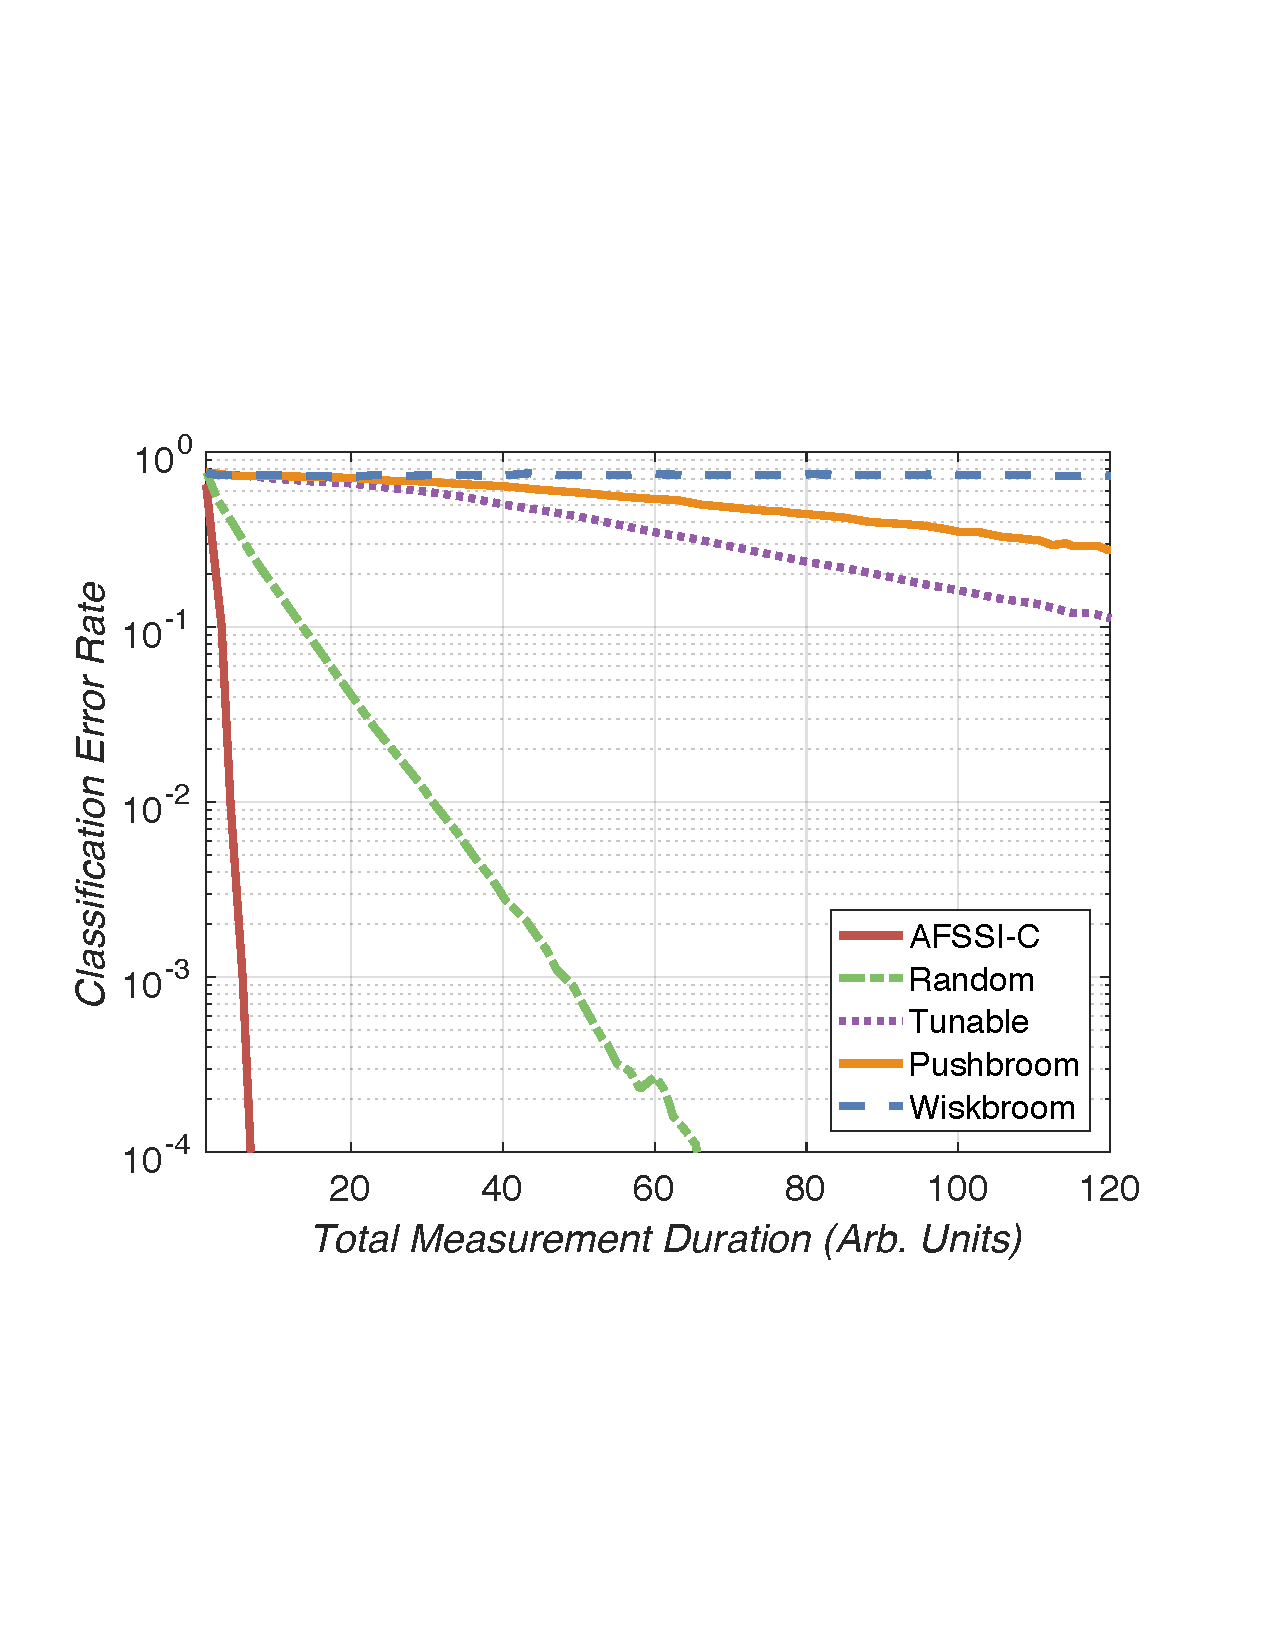
\includegraphics[scale=0.85]{afssicVsOtherSpectromers}\\
  \caption{Simulation comparing the classification performance for different measurements at TSNR = 0 for different systems: the \gls{afssi-c} with designed features (joint pPCA), the \gls{afssi-c} with random features, the traditional pushbroom imager, the traditional tunable filter imager, and the traditional whiskbroom imager. The input is a $64 \times 64 \times 38$ spectral datacube with a 4-class library.} \label{fig:afssicVsOtherSpectromers}
\end{figure}
%
There are a number of phenomena which give the \gls{afssi-c} an advantage over traditional systems. When comparing the \gls{afssi-c} system with joint-pPCA designed features to traditional systems at the 5\textsuperscript{th} measurement in \Cref{fig:afssicVsOtherSpectromers}, we see that the classification accuracy improves by 250$\,\times$. This improvement in performance is attributed to a combination of factors such as the open aperture architecture of the \gls{afssi-c} design, lack of scanning, and adaptivity. 

\Cref{fig:afssicVsOtherSpectromers} also demonstrates the advantage joint-pPCA. By inspecting the 5th measurement, one can observe a 100$\,\times$ performance gain relative to static, pseudo-random coding. The performance curve for the random coding case is generated by directly classifying from the acquired measurements using an identical Bayesian inference framework. The information processing inequality of information theory~\cite{cover2012elements} guarantees us that the alternative approach of classifying after datacube reconstructions can do no better than direct classification. Thus, the difference of these two curves represents the actual classification performance improvement due to adaptivity, while the separation between the static-coded curve and the traditional systems represents the performance improvement arising from the increased open aperture. The simulated results show that the \gls{afssi-c} system to outperform traditional systems where classification is the desired result of the analysis.


\section{Conclusion}

In this chapter, I discussed the \acrfull{afssi-c}, a spectral imager classifier that utilizes adaptive spectral features in a low \acrfull{swap-c} configuration. My collaborators and I were able to show multiple order-of-magnitude improvement in classification accuracy compared to traditional spectral imaging systems when the noise in the system is equal to the minimum separation between the library spectra, by employing a system simulation corroborated with experimental results. By taking advantage of its adaptiveness, the \gls{afssi-c} performance with designed features also achieves multiple order-of-magnitude improvement over a random feature implementation. These adaptive features are designed via Bayesian inference and a novel joint-probabilistic PCA approach, which drives the measurement decision evolution to boost the discrimination ability between spectra candidates at every spatial location. 

Direct classification is a useful modality for many of the applications of spectral imaging. By making measurements of an encoded datacube instead of explicit measurement of every element, huge performance gains are realized. It is reasonable to imagine the \gls{afssi-c} system being of great benefit to a number of industries that rely on \textit{in situ} material classification. 
\chapter{Computational Spectral Unmixing}\label{chap:Csu}

\section{Introduction}

In \Cref{chap:Afssic}, I argued that spectral classification is the goal of spectral imaging in most cases. However, in certain situations the analyst is interested in quantifying the presence of several materials in a single spatial location from a \gls{mixed spectrum}. Mixed spectra can occur when the sensor is part of a high-altitude platform such as an unmanned aerial vehicle (UAV) or satellite. The large standoff distances between the ground and the instrument result in large spatial resolutions. For example, in the Hyperion Imaging Spectrometer, which is satellite based, the spatial resolution is 30 meters \cite{folkman2001eo}. One cannot reasonably expect a single material to always occupy that large of an area. \Gls{spectral unmixing} is any procedure which attempts to take the measured spectrum of a mixed pixel and decompose it into a set of constituent spectra called the \glspl{endmember} and a set of corresponding fractions called the \glspl{fractional abundance}. 

Traditional spectral unmixing requires several seperate steps to quantify the fractional abunances. The isomorphic sensor must spatially or spectral scan the object scene, building the spectral datacube piece by piece. At each step, the restricted aperture or wavelength range rejects a significant fraction of the availiable light. A post-processing step is then used to reduce the size of the data to reduce the computational load. Finally an inversion step is used to compute the fractional abundances. Intuitively, the advantages of computational sensing discussed throughout this dissertation should be able to ameliorate some of the design trade-offs in traditional spectral unmixing.

In this chapter, I will talk about my efforts to apply the techniques of computational sensing to directly estimate the \gls{fractional abundance} without the need to reconstruct the spectral datacube. I will introduce a computational spectral imaging architecture called the \gls{lcsi}. I will then provide simulation results that demonstate the advantage of computational spectral unmixing using the \gls{afss} and the \gls{lcsi} over traditional architectures by leveraging the Fellgett and Jacquinot advantage with compressive sensing algorithms which promote sparse solutions. Results from a proof-of-principle experiment demonstrate the promise of computational spectral unmixing. 

\section{The Linear Mixing Model}

There are two main reasons why mixed spectra occur \cite{keshava2002spectral, keshava2003survey}. First, if the spatial resolution of the sensor is low enough, separate materials can jointly occupy the \acrfull{fov} of a single pixel, the resulting spectral measurement is a combination of the constituent spectra, see \Cref{fig:linearAndNonlinearMixing}(a). In this case, one can imagine the object scene as a \emph{checkerboard} mixture: light from the illumination source scatters or reflects from only one of the materials before being observed by the sensor, multiple scattering between materials are ignored. The second reason for mixed pixels occurs when different materials are combined into a homogeneous mixture, see \Cref{fig:linearAndNonlinearMixing}(b). In this case, mixed spectra are not caused by poor spatial resolution, they are inherent to the nature of the scene. For the purposes of this chapter I will focus on the first case, mixed spectra causes by the spatial resolution limitations of the sensor.

\begin{figure}
	\centering
	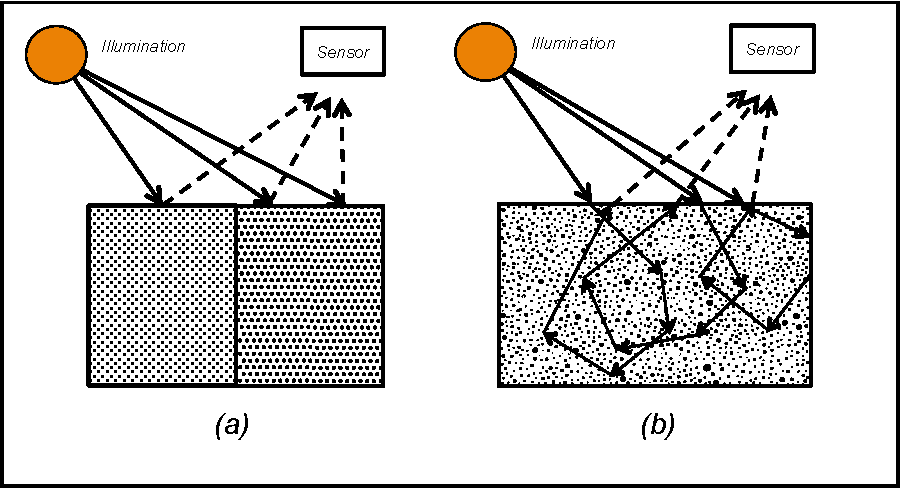
\includegraphics[scale=0.85]{linearAndNonlinearMixing.pdf}
	\captionof{figure}[Linear versus Non-Linear Mixing]{(a) Illustration of linear mixing where incident solar radiation reflects from a surface and the surface consists of distinct materials. (b) Illustration of nonlinear mixing where incident solar radiation encounters an intimate mixture of materials, reflecting or scattering multiple times before being reflected toward the spectral image sensor.}
	\label{fig:linearAndNonlinearMixing}
\end{figure}

When mixed spectra occur due to the spatial resolution limitation of the instrument, the fractional abundance is linearly proportional to the relative area of each material. This is called the \acrfull{lmm}, where the mixed spectrum can be written as 
%
\begin{equation}
\mb{f} = \sum_{r=1}^{N_{R}} x_r \mb{s}_r + \mb{e} = \mb{S} \mb{x}  + \mb{e}
\end{equation}
%
where $\mb{f}$ is the \gls{mixed spectrum}, $\mb{s}_r$ is the $r^{th}$ endmember spectrum, $\mb{S}$ is a matrix in which the columns are the endmember spectra, $\mb{x}$ is the fractional abundance vector, and $N_{R}$ is the number of endmembers in the endmember library, each spectra has \gls{numspecchan} spectral channels. In the \gls{lmm}, the interactions between distinct endmembers are assumed to be neglible \cite{clark1984reflectance}. 

There are two contraints imposed by the physics of the situation. Intuitively we should expect that the fractional abundance should be equal to or larger than zero. This is the \emph{nonnegativity} constraint:
%
\begin{equation}
	x_r \geq 0.
\end{equation}
%
We should also expect that if energy is conserved, i.e. there is no absorption of light, then the \gls{fractional abundance} should sum to one. This is the \emph{additivty} constraint:
%
\begin{equation}
	\sum_{r = 1}^{N_{R}} x_r = 1
\end{equation}


\subsection{Unmixing in Traditional Spectral Imaging}

In traditional spectral imaging, the spectral datacube is first isomorphically acquired by the instrument before any unmixing step is performed. Often a \gls{dimensionality reduction} step is used to reduce the computational burden of processing the spectral datacube \cite{keshava2002spectral, keshava2003survey}. If the endmembers are unknown, an \gls{endmember determination} step is executed. Finally, the \gls{inversion} step is used to estimate the fractional abundances. 

Notable data reduction algorithms include \acrfull{pca} and \acrfull{mnf}. As described in Chapter 2, \gls{pca} is applied to the measured data and finds the basis which decorrelates the data. In \gls{pca} one typically observes a steadily decreasing signal-to-noise ratio as the principal compenent number increases \cite{green1988transformation}. However, this is not always the case, since it equates variance with information and is based on the assumption that the data structure can be described by a multi-dimensional normal distribution \cite{philpot2015mnf}. In \gls{mnf}, the algorithm attempts to order the components in terms of \gls{snr} which consists of two seperate \gls{pca} rotations and a noise whitening step. \gls{mnf} requires estimation of the noise covariance matrix in addition to the covariance of the data.

%A non-statistical technique for dimensionality reduction is the optical real-time adaptive spectral identification system (ORASIS) \cite{bowles2007optical}, which is a series of steps that identify a subset of representative, or exemplar, pixels that convey the variables in a scene. When a new pixel is collects from the scene, a spectrum is compared to each examplar pixel using this angle metrix. If it is sufficently different then it is added to the set. Then using a modified Gram-Schmidt process, an orthogoal basis is created and a new dimension is added until the every exemplar can be represented well within a certain tolerances \cite{keshava2003survey}. 

The inversion step actually estimates the \gls{fractional abundance}. There are a variety of inversion techniques which actually attempt to estimate the fractional abundance vector. Many are based on minimizing the squared error and attempt to enforce additivity or non-negativity \cite{keshava2003survey, lawson1995solving}. There are various algorithms based on \acrfull{map}, \acrfull{mle}, and clustering which can be used for spectral unmxing. Unfortunately, we cannot explore each inversion technique, however due to their prevalence, I will use least-squares based inversion technique when comparing computational spectral unmixing techniques to tradiational unmixing techniques.

\section{Architecture}

In this research, two seperate architectures are used for spectral unmixing. The first architecture is the \gls{afss}, which is the single pixel version of the \gls{afssi-c} described in depth in \Cref{chap:Afssic}. The second architecture is a \acrfull{lcos} based spectral imager, called the \gls{lcsi}, which allows for an extremely compact instrument, see \Cref{fig:lcsiArchi}. The system provides a programmable spectral filter, which can be independently addressed at each physical pixel of the \gls{slm}. The device consists of an array of micro cells of liquid crystal on a reflecting layer \cite{lazarev2012lcos}. Each layer of liquid crystal can be modeled as a thin retarder plate. Since the birefringent phase retarder is sensitive to wavelength, the \gls{lcos} combined with a polarizing beam splitter or a linear polarizer produces a wavelength dependent transmission pattern, a spectral filter, which modulates the input spectra \cite{yuan2015compressive}.

\begin{figure}
	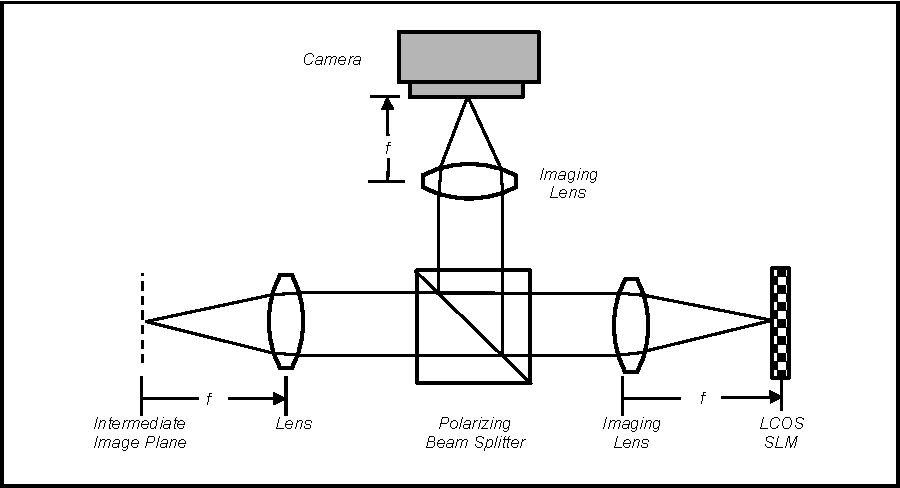
\includegraphics[scale=1.0]{lcsiArchi.pdf}
	\captionof{figure}[LCOS Based Spectral Imager]{The LCOS Spectral Imager. Light from the intermediate image plane is collimated. A polarizing beam splitter passes p-polarized light and rejects s-polarized light. Upon reflection of the LCOS SLM, the polarization state is changed to some elliptical polarization state. Only the s-polarized portion of the elliptical polarization is reflected toward the upper part where it is imaged onto a scientific camera. The intensity of the light that is passed depends on birefringence created by the programmable LCOS.}
	\label{fig:lcsiArchi}
\end{figure}

%\subsection{How the LCOS Creates Spectral Filters}
% Imagine an incident monochromatic plane wave traveling in the z-direction with a Jones polarization vector 
% \begin{equation}
% \mbh{a} = 
% 	\begin{bmatrix}
%     	a_{x}  \\
%     	a_{y} e^{ i \phi  }  \\
%    \end{bmatrix}
% \end{equation}
% %
% where $\phi$ is the phase differene between the x and y axes \cite{milster2013notes}. The full plane wave for the electric field can be written as

% \begin{equation}
% \mb{E} = A \exp \left[ \mb{k} \cdot \mb{r} - \omega t \right] \mbh{a}
% \end{equation}
% %
% where there leading $A$ is a complex constant that adjusted for amplitude and absolute phase shift.
% %
% \begin{equation}
% 	\mb{k} = k \mbh{k} = k \ap{ \alpha \mbh{x} + \beta \mbh{y} + \gamma \mbh{z} }
% \end{equation}
% %
% is the propagation vector with wavenumber $k = 2\pi /\ \lambda$ and direction cosines $\ap{\alpha, \beta, \gamma}$.

% Transmitting through the polarizing beam splitter only passes horizontally polarized light

% \begin{equation}
% 	\begin{bmatrix}
% 		a_x \\
% 		0 
% 	\end{bmatrix}
% 	=
% 	\begin{bmatrix}
% 		1 & 0 \\
% 		0 & 0
% 	\end{bmatrix}
% 	\begin{bmatrix}
% 		a_x  \\
% 		a_y e^{ i \phi  }
% 	\end{bmatrix}
% 	\label{eq:jonesAfterPBS1}
% \end{equation}

% The \gls{lcos} in our architecture is a phase only reflective type. Liquid crystal is used because it has the ability change birefringence $\Delta n$ when an electric field is applied. Birefringence is defined as 
% %
% \begin{equation}
% 	\Delta n = n_e - n_0
% \end{equation}
% %
% where $n_0$ is the ordinary refractive index and $n_e$ is the extraordinary refractive index \cite{zhang2014fundamentals}. By changing the electric field in the cell the $\Delta n$ is changed. 

% Birefringence is utilized to create retardation plates. These retardation plates serve to change the polarization state of input light. If one aligns the retardation plate so that the x polarized light is incident on the ordinary refractive index and the y polarized light is incident onto the ordinary refractive index then x and y polarizations are phase shifted by
% %
% \begin{equation}
% 	\eta = \frac{2 \pi}{\lambda} \left[ n_e\ap{\lambda} - n_o \ap{\lambda} \right] T
% \end{equation}
% %
% where $T$ is the physical thickness of the plate, where the $ n_e \ap{ \lambda } $ and $ n_o \ap{\lambda} $ are index of refraction of the extraordinary and ordinary waves which are wavelength dependant functions \cite{milster2013notes}. 

%The general Jones matrix for an arbitrary birefringent material as a retardation plate is
%
%\begin{equation}
%	\begin{bmatrix}
%		M_{11} & M_{12} \\
%		M_{21} & M_{22}
% 	\end{bmatrix}
% 	=
% 	\begin{bmatrix}
% 		e^{i \eta/2} \cos^2 \theta + e^{-i \eta/2} \sin^2 \theta & \ap{ e^{i \eta/2} - e^{-i \eta/2} } e^{-i \phi} \cos \theta \sin \theta \\
% 		\ap{ e^{i \eta/2} - e^{-i \eta/2} } e^{i \phi} \cos \theta \sin \theta & e^{i \eta/2} \sin^2 \theta + e^{-i \eta/2} \cos^2 \theta
% 	\end{bmatrix}
% 	\label{eq:arbJonesMatrix}
% \end{equation}
% %
% where the relative phase retardation between the fast and slow axes is given by $\eta = \phi_y - \phi_x$, $\theta$ is the orientation of the fast axis with respect to the x-axis, and $\phi$ is the circularity. Thus after propagating from the LCOS the Jones Vector is written as
% %
% \begin{equation}
% 	\begin{bmatrix}
% 		a_x M_{11} \\
% 		a_x M_{21}
% 	\end{bmatrix}	
% \end{equation}
% %
% finally the vertical polarization (y) is reflected by the polarizing beam splitter towards the camera
% %
% \begin{equation}
% 	\begin{bmatrix}
% 		0 \\
% 		a_x M_{21}
% 	\end{bmatrix}	
% \end{equation}

% Where the intensity is pro



% The phase shift can be used to change the polarization state of the light. For example, when linearly polarized light at 45 degrees goes through a phase shift of $\Delta = \lambda / 2$ the polarized light will rotate to vertical. However, this is a special case and in general the output light will be elliptically polarized. When elliptically polarized light is incident onto a linear polarizer, only linearly polarized light is passed, the intensity of the light passed however depends on the relative amplitude and phase of the x and y polarizations of the incident light \cite{milster2013notes}. 

Unfortunately, a full discussion of polarization is not appropriate for this dissertation. The important point is that for light of a single wavelength, the \gls{lcos} produces polarization which in general is not linearly polarized. Placing a linear polarizer after the light has been reflected from the \gls{lcos} will then force the transmitted light to be linearly polarized but at an intensity that depends on the projection of the output polarization from the LCOS onto the transmission direction of the polarizer. Passing non-monochromatic light to an \gls{lcos} and then a linear polarizer will impart a wavelength dependent intensity. In short, the \gls{slm} provides polarization and wavelength dependent transmission patterns to encoded the spectral datacube \cite{tsai2015spatial}.

\subsection{Forward Model}

The forward model for the \gls{lcsi} is similar to the forward model for the \gls{afssi-c} presented in \Cref{ssec:afssicForwardModel}, except now one does not need to account for the dispersion when imaging from the input plane to the LCOS and from the LCOS to the \gls{fpa} of the camera. I will thus skip the derivation of the forward model and simply present the final equation for the measurement value at pixel $n$ and $l$ from the camera:
%
\begin{align} 
	\Gamma_{nl} &= \sum_{n^\prime l^\prime} \iiint \mbox{rect} \left( \frac{x}{\Delta} - l, \frac{y}{\Delta} - n \right) \mbox{rect} \left( \frac{x}{\Delta} - l^\prime , \frac{y}{\Delta} - n^\prime \right) \notag \\
 	&\qquad \times T_{n^\prime l^\prime} \ap{\lambda} D_0 \left( x, y; \lambda \right) dx \, dy \, d\lambda.
\end{align}
%
Notice that there is no dispersion constraint like the one created in the \gls{afssi-c} or a joint spatial-spectral contraints like in the \gls{cassi}. The \gls{lcos} creates dispersion by the very nature of wavelength dependant birefringence. If one so choose to, one can simply treat each pixel in the image as completely indepdent from neighboring pixels. This greatly simplifies the analysis. 

Similar to the \gls{afssi-c} we can further simplify this by imagining a discrete spectral density, the spectral datacube. The discretized source spectral datacube is $D$, and then the detector signal $\Gamma$ is a result of spectral filter created by the \gls{pbs} and LCOS combination where spectral filter $T$ acting on the pixelated source is
%
%
\begin{equation}
	\Gamma_{n,l} = \sum^{N_{\lambda}-1}_{c = 0} T_{n,l,c} D_{n,l,c} \,
\end{equation}
%
%
which shows the measurement at each pixel being the inner product of the source spectrum and the spectral filter created by the \gls{pbs}-\gls{lcos} combination. In a single spatial location, this reduces to a simple inner product
%
\begin{equation}
	g_m = \mb{h}_m^{T} \mb{f} 
\end{equation}
%
where the subscript $m$ represents the $m^{\text{th}}$ measurement step and $\mb{f}$ the true spectrum at that pixel. For a sequence of measurements this simplies to 
%
\begin{equation}
	\mb{g} = \mb{H} \mb{f}
\end{equation}
%
where the $m^{th}$ row of $\mb{H}$ is $\mb{h}_m^T$ and $\mb{g}$ is an $N_m \times$1 vector, $\mb{f}$ is the ground truth mixed spectrum
%
\begin{equation}
	\mb{f} = \mb{S}\mb{x}
\end{equation}
%
Thus for a sequence of noisy measurements at a single pixel
%
\begin{equation}
	\mb{g} = \mb{H}\mb{S}\mb{x} + \mb{e} = \mb{A}\mb{x} + \mb{e}
\end{equation}\label{eq:csuForwardModel}
%
where $\mb{H}$ is an $N_m \times N_{\lambda}$ matrix, $\mb{S}$ is the endmember library which is an $N_{\lambda} \times N_{R}$ matrix, $\mb{x}$ is the fractional abundance vector which an $N_R \times 1$ vector, $\mb{e}$ is the additive noise which is a $N_m \times 1$ vector. If I define
%
\begin{equation}
	\mb{A} = \mb{H} \mb{S},
\end{equation}
%
One can think of $\mb{H}$ as the sensing matrix and $\mb{S}$ as the representation matrix as discussed in \Cref{sec:compressiveSesing}.


\section{Solving the Inverse Problem}

For this work I chose to use the least-squares estimator (LSE)
%
\begin{equation}
	\mbh{x} = \ap{ \mb{A}^T \mb{A} }^{-1} \mb{A}^T \mb{g}
\end{equation}\label{eq:lseEquationChap5}
%
to demonstrate the advantage provided by multiplexing without using compressive sensing based algorithms. To demonstrate compressive sensing approaches, I will used the built-in MATLAB \texttt{lasso} function which attempts to minimize the $\ell_1$ regularized least-squares objective function 
%
\begin{equation}
	\mbh{x} = \argminA_{\mb{x}} \: \| \mb{Ax} - \mb{g} \|_{2}^{2} + \tau \| \mb{x} \|_1
	\label{eq:l1reglsV2}
\end{equation}
%
in order to find fractional abundances that are sparse. 

In the traditional spectral imager, the fractional abundance is estimated after the spectral datacube is acquired. In our work, the fractional abundance can be estimated after each measurement step. However, since we need a way to compare our results to traditional spectral imaging, we can use the tunable filter architectures for a baseline comparision. The tunable filter acquires a single wavelength over the entire field-of-view and thus allows us to obtain measurements in a time sequential manner. This means that we can use the LSE to get an idea of how a traditional spectral imaging architecture would perform.

As I mentioned earlier, in remote sensing the fractional abundance vector $\mb{x}$ tends to be sparse: the number of endmembers in the library is much larger than number of endmembers that are actually present in the mixed spectrum $N_{R} > \| \mb{x} \|_0$. Therefore, one can invoke the techniques designed for compressive sensing to find solutions that are sparse.

\section{Prior work}


\subsection{Prior Efforts in Computational Spectral Unmixing}

Several researchers have shown promising results in applying compressive sensing to spectral unmixing using a modified single-pixel camera architecture \cite{li2012compressive}. They demonstrated the ability to reconstruct the fractional abundance planes without the need to explicitly reconstruct the spectral datacube. In this approach, the object scene is imaged onto a \gls{dmd} and then a condensor lens focuses the reflected light into a whiskbroom spectrometer. One can think of this architecture as a set of parallel single-pixel cameras each operating at a different spectral channel, with the constraint that each \gls{dmd} must display the same pattern. This architecture does not code the spectral dimension of the spectral datacube. The researchers demonstrated compressive unmixing by minimizing the total variation (TV) of the endmember images while enforcing the nonnegativity constraint. 

In another effort, researchers use the \acrfull{cassi} architecture to perform compressive sensing on the spectral datacube and solve the $\ell_1$-regularized least squares problem (lasso in regression) to promote sparsity in the fractional abundances \cite{monsalve2015spectral}. Due to the nature of the single-disperser \gls{cassi} architecture, the researchers are forced to solve a larger joint-inference problem to preform spectral unmixing. 

\subsection{Prior efforts using LCOS Computational Spectral Imaging}

Several groups have previously demonstrated computational spectroscopy and spectral imaging results using variations of liquid crystal technology. The first instance, in 2012, used a single-pixel liquid crystal device to demonstrate compressive spectroscopy and exhibited a 10$\times$ reduction in the number of measurements compared to a traditional ismorphic spectrometer \cite{august2013compressive}. Shortly after in 2013, a demonstration of a compressive spectral imager using an \gls{lcos} \gls{slm} was published which jointly coded spatial and spectral features \cite{zhu2013coded}. In 2015, an \gls{lcos} based hyperspectral imaging sensor demonstrated blind compressive sensing, using a Bayesian approach to dictionary learning \emph{in situ} \cite{yuan2015compressive}. That same year, a miniture ultraspectral imaging system based on a custom built liquid crystal cell, which applies the same spectral filter to each spatial location, demonstrated the ability to reconstruct gigapixel spectral datacubes with an order of magnitude reduction in measurement steps compared to isomorphic systems \cite{august2016miniature}. However, to my knowledge, no one has ever attempted to perform direct spectral unmixing using an \gls{lcos} based device. 


\section{Design and Selection of Spectral Filters for Unmixing}


\subsection{Adaptive Unmixing Algorithm For the AFSSI-C}\label{sec:unmixingAlgo}


The \acrfull{afss} has the ability to display psuedo-arbitrary spectral filters with the restriction of using binary codes $ \{ -1, +1 \}$ using the \gls{dmd}. In the \gls{afss}, one can emulate a tunable filter spectrometer by measuring one spectral channel at time, i.e. turn on one mirror per measurement step. In this case, the measurement matrix is equal to the identity matrix $\mb{H} = \mb{I}$. Combining the tunable filter approach with the LSE produces what one should expect from a traditional isomorphic spectrometer to conduct spectral unmixing.

We can also use random binary codes to achieve a multiplexed measurement to improve the throughput of each measurement to reduce the unmixing error. The spectrum can then be estimated by processing the measurement with the LSE to demonstrate the performance gained by collecting more light per measurement step. However, estimating the fractional abundance using a compressive sensing based algorithm such as the MATLAB \texttt{lasso} function can produce even better unmixing results by enforcing sparsity. 

As shown in the \gls{afssi-c}, adaptive coding can significantly improve performance compared to multiplexing alone. We developed an algorithm for adaptively creating spectral filters which uses a modified version of \gls{ppca} to create adaptive spectral filters. This algorithm begins with the spectral library which consist of the each endmember spectra $\mb{S}$. Initially, before any measurements are made, the estimated fractional abundance of each endmember is assumed to be the same: 
%
\begin{equation}
	\mbh{a}_{m=0} = 
	\begin{bmatrix}
	\frac{1}{N_R} \\
	\frac{1}{N_R} \\
	\vdots \\
	\frac{1}{N_R}
	\end{bmatrix}
\end{equation}
%
where $N_R$ is the number of endmembers. The subscript denotes the $m^{th}$ measurement step. Before any measurement is made, $m=0$. Then each endmember in the spectral library is weighted by the square of their respective estimated fractional abundance
%
\begin{equation}
	\mb{S}_w = 
	\begin{bmatrix}
		\hat{a}_1^2 \mb{s}_1 & \hat{a}_2^2 \mb{s}_2 & \hdots & \hat{a}_{N_R}^2 \mb{s}_{N_R}
	\end{bmatrix}
	\label{eq:weightedSpectralLibrary}
\end{equation}
%
this is called the weighted spectral library. Then the eigenvectors of the unnormalized covariance matrix of the weighted spectral library are computed to obtain the principal components
%
\begin{equation}
	\mb{X}_m = \mb{S}_w \mb{S}_w^T.
\end{equation}
%
Where the first principal component corresponds to the direction of largest variance and so on. Initially, for the first measurement, the algorithm chooses the first principal component for the spectral filter $\mb{h}_{m=1} = \mb{p}_1$. The measurement is then recorded
%
\begin{equation}
	g_{m=1} = \mb{h}_{m=1}^{T} \mb{f} + e_{m}
\end{equation}
%
A simulated ``guess'' measurement based on the current estimated fractional abundance $\mbh{a}_{m -1}$ is also computed:
% 
\begin{equation}
	\gamma_{m=1} = \mb{h}_{m=1}^{T} \mb{S} \mbh{a}_{m=0}
\end{equation}
%
notice that the guess measurement does not include any simulated noise. Remember $\mb{S}$ denotes the original spectral library matrix, not the weighted spectral library matrix. After the measurement is recorded, the $\ell_2$ norm of the difference between the guess measurement and the actual measurement is recorded:
%
\begin{equation}
	\xi_m = \| \gamma_m - g_m \|_2 
\end{equation}
%
The fractional abundance is then estimated using the MATLAB \texttt{lasso} function. In practice, the LSE is used for the first measurement step since the function \texttt{lasso} requires atleast two rows for $\mb{A}$ and therefore two measurements, to run. 

The spectral library is then reweighted using \Cref{eq:weightedSpectralLibrary}. Again the principal components are recomputed. For the $m^{th}$ measurement step, the $m^{th}$ principal component is used for the spectral filter. After the measurement has been recorded, the  $\ell_2$ norm of the difference between the guess measurement and the actual measurement is recomputed $\xi_m$. 

%Again the weighted spectral library is recomputed as well as the principal components. 

This continues after each measurement until either two things happen: 
\begin{enumerate}
	\item If the current $\ell_2$ norm of the difference between the guess and the actual measurement exceeds the last $\ell_2$ norm of the difference between guess and actual measurement by
	%
	\begin{equation}
		\xi_m > \xi_{m-1} - \frac{\sigma}{2}
	\end{equation}	
	%
	where $\sigma$ is the standard deviation of the system noise, which is assumed to be \gls{awgn}.

	\item Used the sixth principal component.
\end{enumerate}

when either of these two conditions are met, the loop resets to using the first principal component again. I constrained the algorithm to only use the first six principal components, because I noticed that the unmixing preformance is optimized when limited to only the first six principal components. Intuitively, this may be occuring because higher principal components tend exhibit lower SNR or because the spectra in the library do not exhibit significant high frequency features. This algorithm is called \acrfull{swpca}. It is important to note that as of yet, this algorithm does not consider the dispersion constraint of the \gls{afssi-c}, and therefore is more appropriate for the single pixel version, the \gls{afss}. The MATLAB code which simulates \gls{swpca} is found in Appendix \ref{app:adaptiveUnmixAlgo}.


\subsection{Hybrid Spectral Filters for the LCSI}\label{ssec:hybridFiltersLCSI}

The spectral filters produced by the \gls{lcsi} architecture are constrained by the physics of the birefringence dispersion created by the \gls{lcos}. For our particular model, the Holoeye PLUTO LCOS SLM, the spectral filter is changed by sending a different grayscale value to the green channel of the video input (Holoeye allows their SLM to be connected like a second monitor). Since there are 256 grayscale values (0-255), there are 256 different spectral filters, see \Cref{fig:slmSpectralFiltersVisible}. 

Since one is not able to design the spectral filters individually, the next best thing is to choose which spectral filters should be used at each measurement step. Intuitively, one can imagine that using the same spectral filter over and over again will lead to a measurement matrix $\mb{H}$ where the rows are linearly dependent. Instead, one should strive to construct a measurement that is highly incoherent to satisfy the \acrfull{rip}. 

For my experiment, I will compare several methods of choosing the spectral filters. The first method is simply selecting them at random from a discrete uniform distribution between 1 and 256, while constraining the selections to prevent using the same spectral filter from being used more than once. This technique however does not attempt to incorporate any prior knowledge about the statistics of the endmembers, besides sparsity. 

One attempt to incorporate the statistics of the endmembers is to use \gls{pca} to select the spectral filters. One could imagine an algorithm which computes the principal components of the endmembers (spectral library) and then selects the spectral filters which most closely resemble the principal component vector $\mb{p}$ based on their angle:
%
\begin{equation}
	\mb{h} = \argmaxA_{\mb{h}} \: \left\{ \frac{ \mb{p} }{ \| \mb{p} \| } \cdot \frac{ \mb{h} }{ \| \mb{h} \|  } \right\}.
\end{equation}
%
For the $m^{th}$ measurement, the spectral filter whose dot product is largest with the $m^{th}$ principal component of the endmember matrix is selected. However, using all the principal components actually increases the unmixing error after a certain amount of measurement steps, as compared to purely random selections. This occurs for several reasons: As the PC number increases, they actually become less informative. Second, principal components tend become more rapidly varying as the PC number increases, the spectral filters generated by the LCOS are in general smoothly varying and become more difficult to match with the higher principal components.

Thus, we created a hybrid spectral filter selection technique that uses \gls{pca} to select the first several spectral filters and then uses psuedo-random selections after a certain number of measurement steps. This balances the ability of \gls{pca} to choose spectral filters that improve the unmixing error at the initial measurement steps while using random selections to ensure the measurement matrix is incoherent enough to satisfy the \gls{rip}.

The hybrid approach to selecting the spectral filters is further extended to use a more advanced version of \gls{pca} called \acrfull{mnf} transform. \gls{mnf} was originally developed to remove noise from multispectral satellite images \cite{green1988transformation} and attempts to select a basis which orders the signal-to-noise ratio of the MNF components. However, \gls{mnf} is also used for Blind Signal Seperation (BSS), which is the seperation of a set of source signals from a set of mixed signals \cite{hundley2001solution}. Instead of computing the principal components, I compute the maximum noise fraction components of the spectral library. I specifically used the noise adjusted principle component analysis (NAPCA) algorithm to compute the MNF of the spectra library which is found in \cite{hundley2001solution}. The algorithm associates rapidly varying parts of the spectral library with noise and assumes the signal is contained in the smoothly varying parts of the spectral library. 

\begin{figure}[H]
	\centering
	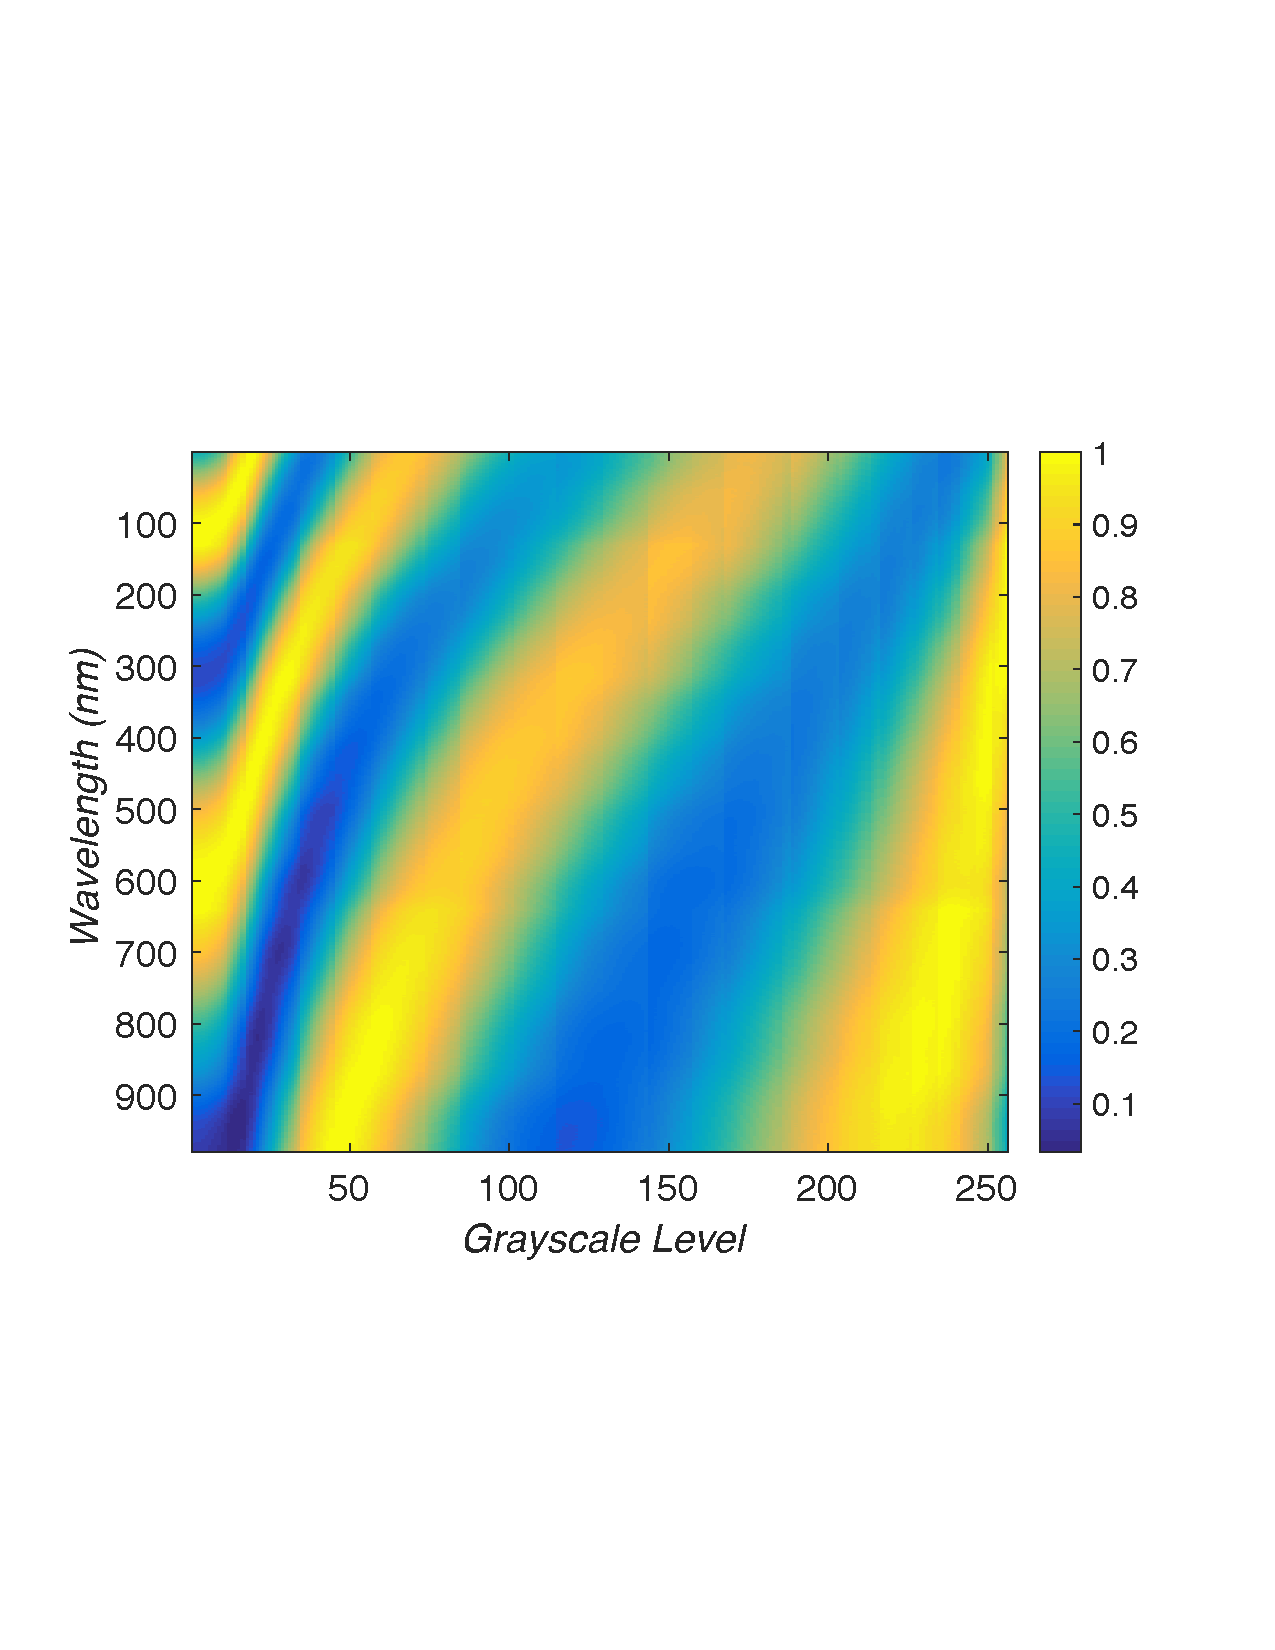
\includegraphics[scale=0.75]{slmSpectralFiltersVisible.pdf}
	\captionof{figure}[The normalized spectral filters created by the Holoeye PLUTO SLM and polarizing beam splitter]{The spectral filters created by the Holoeye PLUTO SLM and polarizing beam splitter. Each column is a spectral filter at a particular grayscale level (0-255) sent to the PLUTO SLM by a custom MATLAB program. }
	\label{fig:slmSpectralFiltersVisible}
\end{figure}


\section{Results}

\subsection{Simulation Results For the AFSS}

Now that I have discussed various coding strategies for spectral unmixing using the \gls{afss}, it is important quantify  them. I performed simulations over five \gls{snr} levels from $10^{-2}$ to $10^2$, where the \gls{snr} is defined as 
%
\begin{equation}
	\text{SNR} = \frac{ \text{E} \Big[ \text{Var}_{N_{\lambda}  \ap{ \mb{s} } } \Big] }{\sigma^2},
\end{equation}
%
which is the ratio of the average variance of the endmembers over the spectral channels to the noise variance. The results after 40 measurement steps are shown in \Cref{fig:unmixingTechniquesComparison}, which show the average \acrfull{rmse} of the estimated fractional abundance versus SNR. \gls{rmse} is defined as 
%
\begin{equation}
	\text{RMSE} =  \left[ \frac{1}{N_R} \sum_{r = 1}^{N_{R}} \ap{ \hat{a}_r - a_r }^2 \right]^{\frac{1}{2}}
\end{equation}
%
The purple dotted line represents the performance of a tunable filter architecture combined with the least-squares estimator (LSE). With random binary patterns, one can obtain an improvement of approximately 3$\times$ which demonstrates the advantage of multiplexing, as shown in the mustard dash-dotted line. By incorporating the prior knowledge of sparsity of the fractional abundance a futher improvement is also achieved, as shown in the orange dashed line. Finally, the blue solid line represents how adaptively designing the spectral filters and using compressive sensing provides an even better result than random coding alone. 

\Cref{fig:unmixingVsMeasurement} shows the average RMSE as a function of measurement number for SNR = 0.01, 1, and 100. The blue line represents psuedo-random spectral filters, the error decreases monotonically with measurement number as one would expect. The green lines represent what happens if the adaptive algorithm never went back to the first principal component once either of the two conditions in \Cref{sec:unmixingAlgo} are met. Simply using higher principle components does not reduce the RMSE after a certain point, even when the spectral library is weighted by the fractional abundance. The red line represents the adaptive algorithm as discussed. This demonstrates the importance of going back to the first principal component whenever the two conditions are met in the adaptive algorithm: it breaks the performance plateau and significantly reduces the unmixing error compared to random coding alone.

\begin{figure}
	\centering
	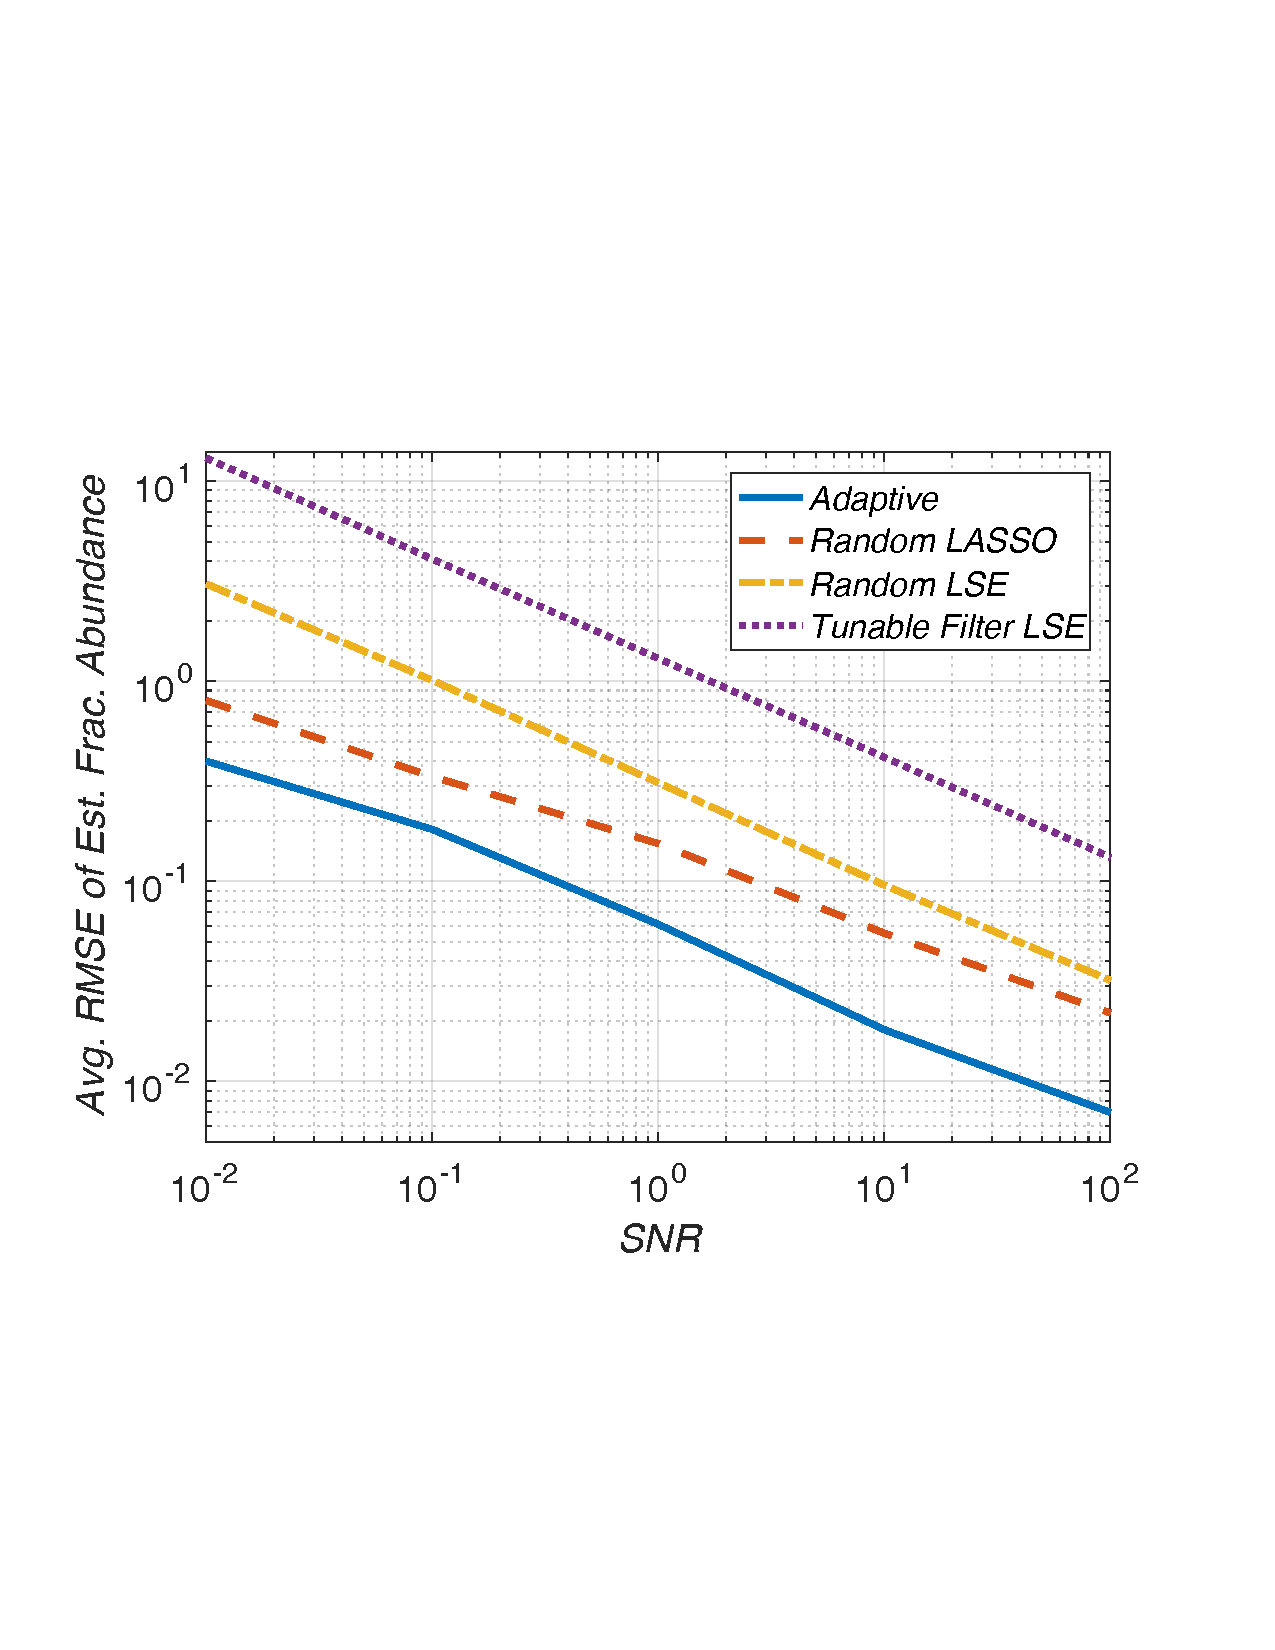
\includegraphics[scale=0.70]{unmixingTechniquesComparison.pdf}
	\captionof{figure}[Comparison of Spectral Unmixing Techniques for the AFSSI-C at five different SNR levels]{A comparison of spectral unmixing techniques for the AFSSI-C at five different SNR levels. The y-axis represents the average RMSE of the estimate fractional abundance. The x-axis represents the signal-to-noise in the measurements. The tunable filter LSE refers to the average unmixing performance if one were to use a tunable filter spectral imaging architectures with least squares estimation to estimate the fractional abundance. The random LSE line refers to the improvement in spectral unmixing This shows the improvement that multiplexing provides over simple tunable filter spectral imaging using the least squares estimator (LSE). Then using the multiplex advantage and algorithms that promote sparsity when the fractional abundance is known to be sparse, one can significantly outperform }
	\label{fig:unmixingTechniquesComparison}
\end{figure}

\begin{figure}
	\centering
	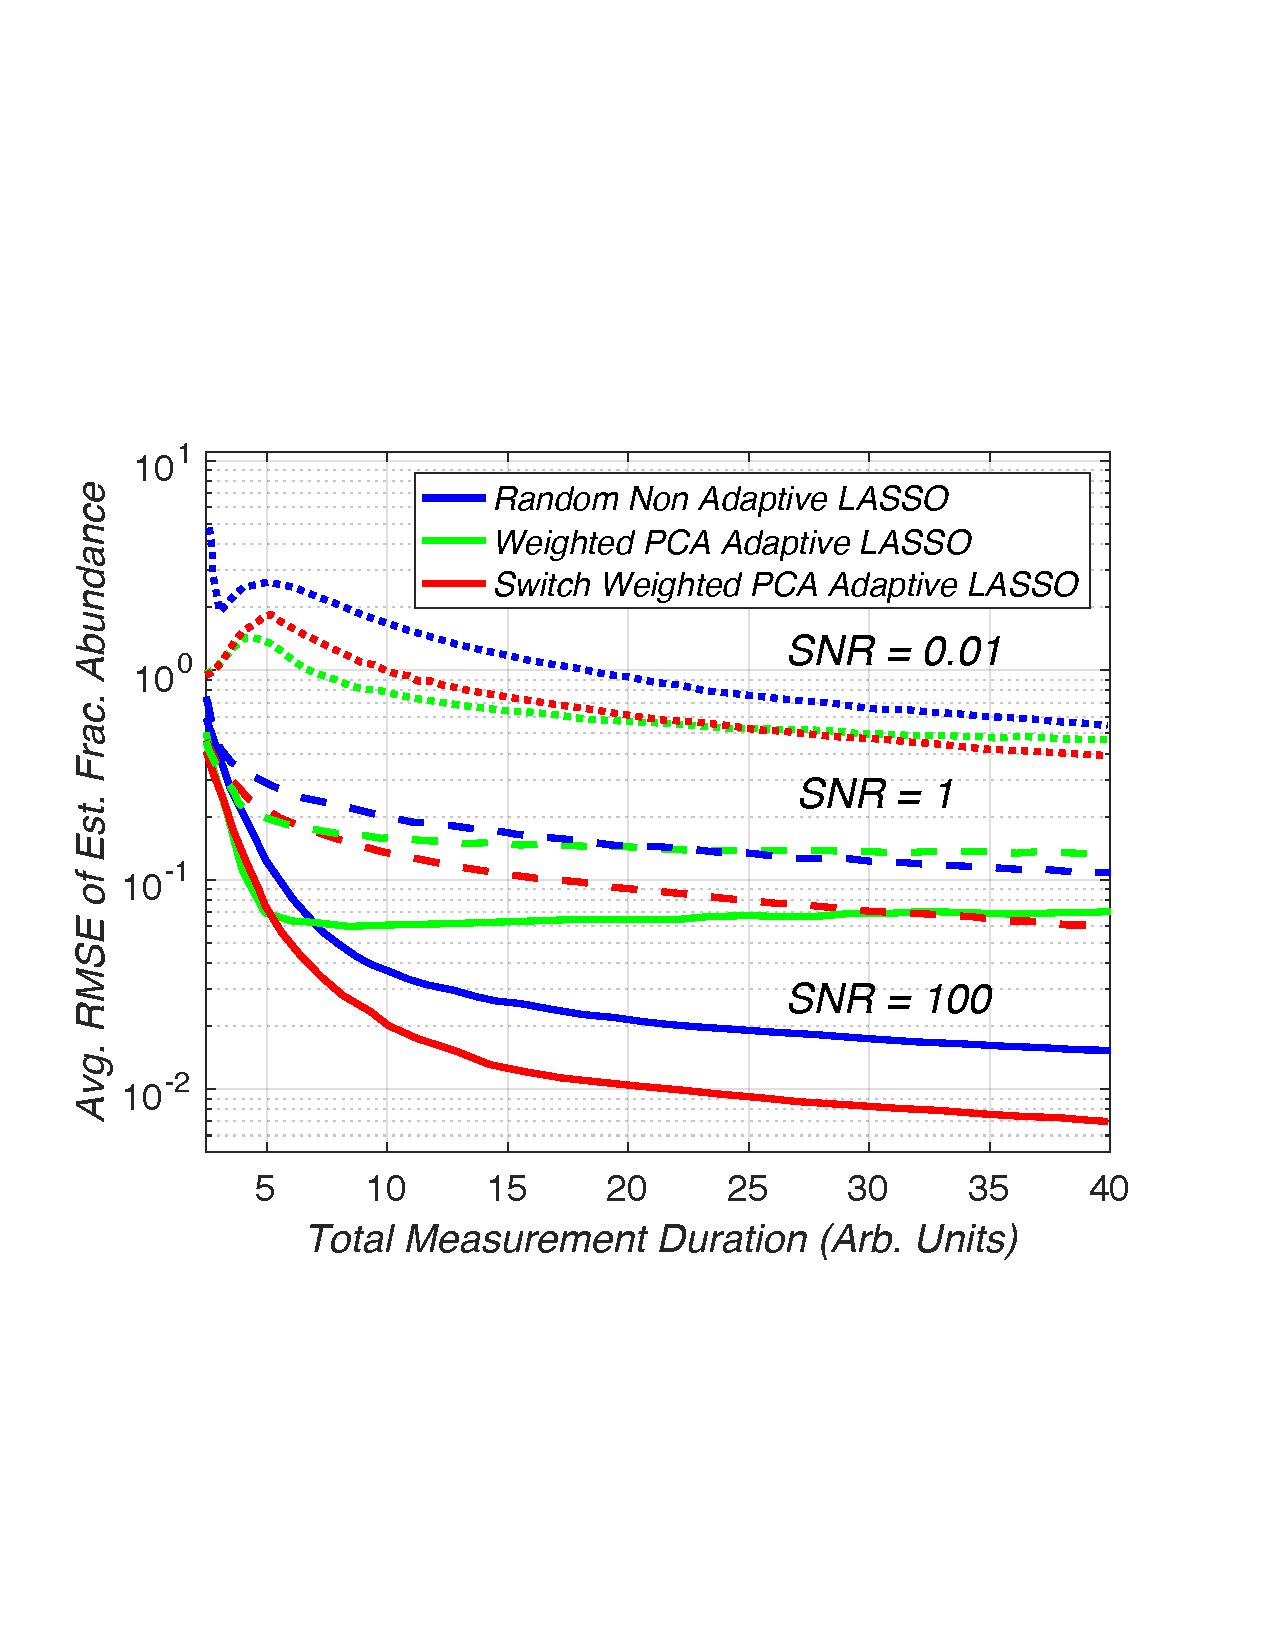
\includegraphics[scale=0.70]{unmixingVsMeasurement.pdf}
	\captionof{figure}[Comparison of Spectral Unmixing Techniques for the AFSSI-C versus Measurement Duration]{Comparison of Spectral Unmixing Techniques for the AFSSI-C versus Measurement Duration for SNR = 0.01, 1.0, and 100. Even though the spectral library is weighted by the fractional abundances from the last measurement, simply using every principal component underperforms using random spectral filters with $\ell_1$ regularized least squares (lasso). Switching the principal components according the algorithm described in \Cref{sec:unmixingAlgo} siginificantly reduces the unmixing error. }
	\label{fig:unmixingVsMeasurement}
\end{figure}


\subsection{Initial Experimental Results of Compressive Unmixing Using the AFSSI-C}

I performed an initial proof-of-principle experiment using the \gls{afssi-c} architecture. Due to the dispersion contrainst of the AFSSI-C, I was unable to test the adaptive algorithm, however the random coding and the use of sparsity promotting algorithms can still be demonstrated. 


For this experiment I had to upgrade the \gls{afssi-c} prototype by adding a second display, see \Cref{fig:unmixingArch1}. This is because the original prototype used only one LED computer monitor, so it can only display combinations of the same red, green, and blue (RGB) spectra, producing only three endmembers. In order to have six endmembers, I added an OLED display which also has red, green, and blue spectra but are different enough that they are not simply scaled versions of the RGB spectra from the LED monitor. This is shown in \Cref{fig:unmixingLibrary}. Note that the RGB spectra from the LED look different from \Cref{fig:afssicSpecLib} which was used for the \gls{afssi-c} experiment because the transmission from the pelicle beam splitter also acts as a spectral filter. 

\begin{figure}
	\centering
	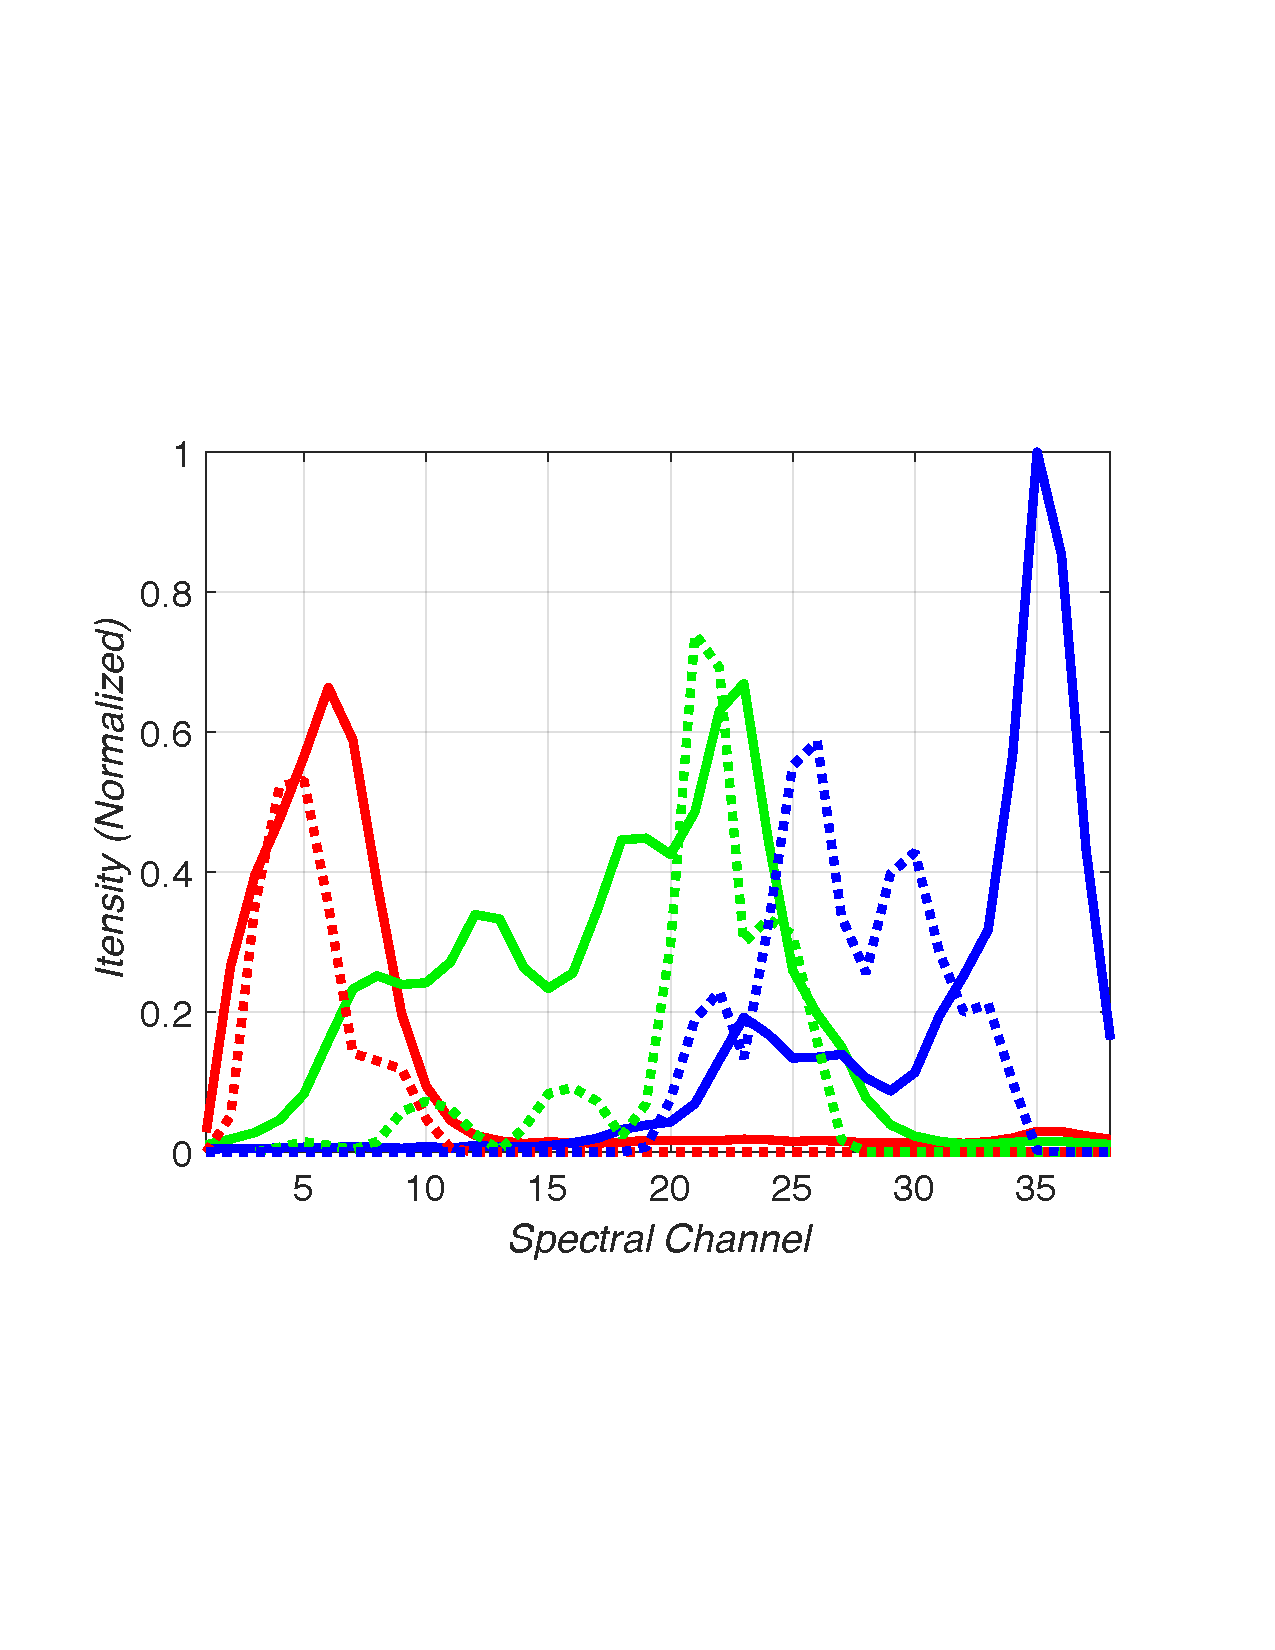
\includegraphics[scale=0.70]{unmixingLibrary}
	\captionof{figure}[Six Endmember Spectra Used For Spectral Unmixing Experiment]{The six endmember spectra used for the spectral unmixing experiment. The library consist of the red, green, and blue spectra from an LED Monitor and the red, green, and blue spectra from the OLED. The LED monitor spectra may look different from the one shown in Chapter 4 since the spectra have been modified by transmitting through a pellicle beam splitter. }
	\label{fig:unmixingLibrary}
\end{figure}

\begin{figure}
	\centering
	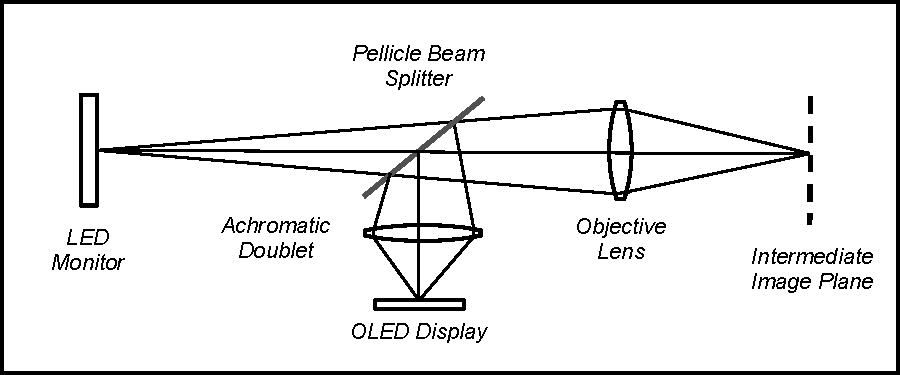
\includegraphics[scale=1.00]{unmixingArch1.pdf}
	\captionof{figure}[Unmixing Architecture for Spectral Unmixing Experiment]{Experimental architecture used to superimpose the spectral images from the LED monitor, which already was in place, and an OLED display. ZEMAX was used to find the correct location of the achromatic doublet, OLED display, and pellicle beam splitter to ensure the intermediate image from both displays appeared at the same location and with the same transverse magnification.}
	\label{fig:unmixingArch1}
\end{figure}

The first-order optical architecture of the unmixing setup was carefully determined using a ray tracing and optimization software package called Zemax. The goal was to ensure that the intermediate image of the LED monitor and the intermediate image of the OLED were at the same location with the same image size. The two images effectively creates a single image which has spectrally mixed pixels with six possible endmembers. The pellicle beam splitter has a clear aperture of 2 inches, thus it needed to be close enough to the objective lens to minimize vignetting. A commercial off-the-shelf 120 mm EFL achromatic doublet from Edmund optics was placed between the OLED and the pellicle beam splitter to move the OLED closer to the instrument. Once all the optical components were optimized in Zemax, they were exported to Solidworks, see \Cref{fig:solidworksOfMixingSetupPicture}, where mounts for the achromatic doublet and the OLED display were designed for 3-D printing. 

There were several practical experimental issues that had to be addressed. Once the setup was constructed, I used a similar spectral calibration procedure from the \gls{afssi-c} experiment to determine the endmembers from the OLED display. The spatial calibration procedure was identical. The OLED was much brighter than the LED monitor, when measured by the SBIG camera. Second, even though the setup was optimized in Zemax, the actual alignment was imperfect. This caused the right side of the OLED to have a larger point-spread function than the left side of the monitor, which caused spatial cross-talk between neighboring pixels. To compensate for this, only one-fourth of the physical pixels were used in a single system pixel. Then a neutral density filter was placed front of the OLED to make the system pixel intensity on the same order-of-magnitude as the intensity from a system pixel from the monitor. Since the pellicle beam splitter acts as a partially reflecting mirror for OLED, I had to account for the image flip by writing a custom MATLAB function which accounts for the left-right flip. 

\begin{figure}
	\centering
	\includegraphics[scale=0.75]{solidworksOfMixingSetupPicture.png}
	\captionof{figure}[Computer Aided Design (CAD) drawing of experimental mixing setup.]{Computer Aided Design (CAD) drawing of experimental mixing setup. Various objects have been ``hidden'' to reduce clutter and emphasize the essential objects: the OLED, the custom design mount for the OLED, the achromatic doublet and the custom designed mount for the doublet, the pellicle beam splitter shown in a kinematic mount, the objective lens also in a custom fabricated C-mount lens.}
	\label{fig:solidworksOfMixingSetupPicture} 
\end{figure}

In order to perform an experiment which demonstrates the ability of the \gls{afssi-c} to perform unmixing on spectrally mixed images, I displayed a 32 $\times$ 32 green ramp on the monitor, see \Cref{fig:linearGreenRampImages}(a). The intensity of the green increases from left to right. The opposite image is displayed on the OLED display, see \Cref{fig:linearGreenRampImages}(b), the intensity of the green decreases from left to right. The other four endmembers which consists of the red and blue of each monitor are set to zero. The fractional abundance of green from both displays sum to one over the entire region-of-interest. 


\begin{figure}
	\centering
	\includegraphics[scale=0.75]{linearGreenRampImages.pdf}
	\captionof{figure}[Ground Truth Images for Spectral Unmixing Experiement]{Ground Truth Images for Spectral Unmixing Experiement. (a) A linear green ramp on the monitor. (b) A linear green ramp on the OLED. Remember that the green of each display are different.}
	\label{fig:linearGreenRampImages} 
\end{figure}

At each measurement step, the DMD is commanded to display a binary random pattern. Since the pattern is designed for $\{ -1, +1 \}$ values, I had to display the positive pattern, record the camera measurement, then display the negative pattern, and record another camera measurement, then subtract the negative from the positive camera images. This unfortunately introduces an additional factor of $\sqrt{\sigma}$ of measurement noise into each measurement step. Both the LSE and the MATLAB \texttt{lasso} function are used to estimate the fractional abundance. \Cref{fig:rmseVsMeasurementExperiment} shows the average RMSE versus measurement number over the 32 $\times$ 32 region. Unfortunately, due to time constraints, I was unable to develop a procedure to estimate the noise in the experiment, therefore the results cannot be directly compared to the simulation results. The result after the $40^{th}$ measurement is shown in \Cref{fig:linearGreenRampImagesExpResultMeas40} 

 By looking at an example pixel, see \Cref{fig:unmixingResultLinearGreenRamp3232}, one can see that the experiment properly identified the two endmembers that were actually present out of the six total endmembers and was able to accurately estimate the fractional abundance after five measurements. 


\begin{figure}[H]
	\centering
	\includegraphics[scale=0.65]{rmseVsMeasurementExperiment.pdf}
	\captionof{figure}[Average RMSE of 32 $\times$ 32 Experimental Spectral Unmixing Results Using the AFSSI-C]{32 $\times$ 32 Experimental Spectral Unmixing Results Using the AFSSI-C with random binary spectral filters. The MATLAB \texttt{lasso} function outperforms the least squares estimator as the number of measurements increase. Thus have an opportunity to beat traditional systems using significantly fewer measurements}
	\label{fig:rmseVsMeasurementExperiment} 
\end{figure}

\begin{figure}[H]
	\centering
	\includegraphics[scale=0.65]{linearGreenRampImagesExpResultMeas40.pdf}
	\captionof{figure}[Image of 32 $\times$ 32 Experimental Spectral Unmixing Results Using the AFSSI-C after the $40^{th}$ measurement.]{Image of 32 $\times$ 32 Experimental Compressive Spectral Unmixing Results Using the AFSSI-C after the $40^{th}$ measurement.}
	\label{fig:linearGreenRampImagesExpResultMeas40} 
\end{figure}

\begin{figure}[H]
	\centering
	\includegraphics[scale=0.65]{unmixingResultLinearGreenRamp3232.pdf}
	\captionof{figure}[Single Pixel Experimental Spectral Unmixing Results Using the AFSSI-C]{Single Pixel Spectral Unmixing Results with the AFSSI-C with random binary spectral filters. The MATLAB \texttt{lasso} function correctly identifies fractional abundance of the two green spectra from each display within five measurement steps. The four other spectra are estimated to be zero. }
	\label{fig:unmixingResultLinearGreenRamp3232} 
\end{figure}


\subsection{Simulation Results For the LCSI}

In order to accurately simulate the spectral filters I first performed a calibration procedure to measure how the each grayscale level filters an input spectrum. A high intensity custom-built white LED lamp was used to illuminate the \gls{lcsi}. At the output we placed an Ocean Optics USB 4000 spectrometer. Then the spectrum of the white light filtered by \gls{lcsi} at each grayscale level is recorded. Then the spectrum at each grayscale level is normalized by the maximum intensity at each wavelength which produces the calibration spectral filters shown in \Cref{fig:slmSpectralFiltersVisible}.

 In order to quantify the filter selection techniques discussed in \Cref{ssec:hybridFiltersLCSI}, I also produced several simulations. simulated the filter selection technique for SNR = 100. \Cref{fig:lcsiResults1} demonstrates the three techniques: randomly selecting filters, the hybrid PCA-Random filter selection, and the hybrid MNF-Random filter selection. Randomly selecting the filters adequately reduces the unmixing error monotonically with measurement error as expected. By using PCA to select the first six spectral filters the and then using a psuedo-random filter selection technique for the rest a significant performance gain is obtained wthin the first 20 measurements. As the number of measurement numbers increases, the probability of having used all the same spectral filters increases. At measurement 256, when all the spectral filters have been used, the average RMSE is the same. Using a hybrid MNF-Random filter selection produces an additional reduction in unmixing error.


\begin{figure}[H]
	\centering
	\includegraphics[scale=0.70]{lcsiResults1.pdf}
	\captionof{figure}[Comparing Random and Hybrid Spectral Filter Selections for the LCSI]{Comparing Random and Hybrid Spectral Filter Selections for the \gls{lcsi} at SNR = 100. One cannot generate arbitrary spectral filters with the \gls{lcsi}, therefore one must decide how to select from a set of 255 possible spectral filters. A hybrid of using the spectral filters that are closest in angle to the first six principal components and then using random filter selections outperforms purely random filter selections. Similarly, a hybrid of using the spectral filters that are closest in angle to the \gls{mnf} components for the first six measurement steps and then using random filter selections outperforms the random and the PCA-random hybrid filter selection. }
	\label{fig:lcsiResults1}
\end{figure}

\section{Conclusion}

Computational spectral unmixing is a computational sensing approach to estimating the fractional abundances of mixed spectra without the need to directly reconstruct the hyperspectral datacube. I discussed two separate architectures for spectral unmixing, the \gls{dmd} based \gls{afss} and the \gls{lcos} bases \gls{lcsi}. I developed two seperate approaches for coding the mixed spectral measurements for a compressing sensing approach for unmixing. The first used adaptive spectral filters combined with conditions to prevent the unmixing error from plateauing. The second relies on variation of \acrfull{pca} or \acrfull{mnf} to find spectral filters provide very informative measurements compared to simplying selecting spectral filters at random. Simulations show the viability these techniques to significantly reduce the unmixing error over naively random coding (or filter selection) alone, demonstrating the importance of incorporation the prior knowledge of the statistics of the signal-of-interest. 
\chapter{Conclusion}\label{chap:Conclusion}

This dissertation discussed several important practical considerations of computational sensing and how they are addressed in three separate applications: compressive object tracking, adaptive spectral image classification, and compressive spectral unmixing. As computational sensing continues to make rapid progress in the coming years many of these issues must be addressed and confronted. 

The first chapter introduced the reader to the concepts of isomorphic and computational sensing. Computational sensing was developed from the disparate fields of multiplexing spectroscopy and indirect imaging. However, the development of the \gls{ccd}, the digital computer, and data compression allowed scientists to begin creating practical and reliable demonstrations of computational sensing. The advent of the mathematics and algorithms of compressive sensing generated an additional technological leap which dramatically reduced the number of measurements in order to reconstruct the signal of interest. Once the history and benefits of computational sensing was discussed, I then discussed the practical issues of computational sensors: calibration, over multiplexing due to finite dynamic range and quantization resolution, code design and optimization, and the need for a priori knowledge.

The second chapter formally developed the concepts related to computational sensing. I discussed the Fellgett advantage, using Hadamard and S-matrix multiplexing. Then a formal discussion of \acrfull{pca} was developed, which demonstrates how it can be used as a dimensionality reduction technique which creates a basis that decorrelates the data. Then a formal discussion on Bayesian statistics was given which justified their use in the \gls{afssi-c}. Sparsity, incoherence, and the \acrfull{rip} were discussed in-depth to demonstrate why random coding is popular for acquiring sparse signals in compressive sensing. The $\ell_1$ minimization subject to data agreement constraints and its equivalent problem minimizing the $\ell_1$ regularized least squares objective function were also discussed with some intuition as to why it works well for promoting sparse solutions to undetermined inverse problems. 

The \acrfull{scout} was discussed in the third chapter. The \gls{scout} showed how intentionally blurring the \acrfull{psf} in a compressive imager can actually help reduce the effects of overmultiplexing. As the amount of signals being sensed increases the variations in the sensed single become more difficult to discern. Overmultiplexing occurs due to the finite dynamic range and quantization resolution. In the single pixel camera \cite{duarte2008single}, one is forced to measure a series of projections in a time sequential manner prior to solving an inverse problem, in the \gls{scout} the projections occur in parallel for a single difference scene. The \gls{scout} introduced the reader to the importance of calibration in a compressive sensor. The measurement matrix must be carefully measured to produce optimal results. It also demonstrated that optimizing the measurement matrix can be extremely time consuming by hand. Developing a heuristic method based on the coherence metric and ray based simulations reduced the time it took to find optimal design parameters. 

The fourth chapter discussed the \acrfull{afssi-c} which is a computational spectral image sensor designed to adaptively classify spectra at each location in the field-of-view of the sensor. It used back-to-back spectrographs with a digital micro-mirror device (DMD) to produces psuedo-arbitrary spectral filters at each system pixel. After each measurement, an algorithm updates the probabilities of each spectra and weighted the spectral library before recomputing principal components. The first principal component vector is then used as the spectral filter for each measurement. The \gls{afssi-c} is shown to quickly converge to the correct spectrum significantly outperforming traditional spectral imaging architectures especially in low \gls{tsnr} scenarios. The chapter discussed the development of spatial and spectral calibration procedures, vital for optimal performance of the \gls{afssi-c}. A procedure for estimating the system noise was also described in-depth. 

The fifth chapter discussed an extension of spectral classification called spectral unmixing. Two architectures were discussed for spectral unmixing: the \acrfull{afss} and the \acrfull{lcsi}. The \gls{lcsi} relies on the wavelength dependent nature of birefringence to generate multiplex spectral measurements. One of the major constraints of the \gls{lcsi} is that psuedo-arbitrary spectral filters are not possible like in the \gls{afss} or \gls{afssi-c}, therefore I had to develop techniques for selecting spectral filters using random selections and a hybrid of using \gls{pca} or \gls{mnf} to select spectral filters and then using the random filter selections. 

\section{Future Outlook}


One research project that has been an active area of research in the \acrfull{LENS} is the coded memory effect imaging system being developed by my colleague Xiaohan Li. The project combines the memory effect of speckle with \acrfull{cacti} to temporally code speckle. This allows one to infer dynamic object information that is not directly observable with the speckle alone. 

Computational sensing continues to have an extremely promising future. Large companies are actively conducting research and developing products which take advantage of the principles of computational sensing. For example, Microsoft sells a depth sensor, called the Kinect, which relies on a form computational sensing to infer the distance of objects and their shapes. Meanwhile, a recently announced grant from NASA will fund the development of snapshot hyperspectral imagers based on the \acrfull{ctis} for space-borne applications \cite{ricespectraleyes2016grant}. Many university based research groups around the world are actively conducting research that demonstrate compact spatial, spectral, temporal, and polarization computational sensing. Computational sensing will become even more prevalent as the demand for higher resolutions in resource constrained environments abound. 
%\bibliographystyle{IEEEtranS}  
%\bibliography{ThesisBib}






\begin{appendices}
	\chapter{Derivation of the Least Squares Estimator}\label{app:Derivation of the Least Squares Estimator}


Suppose 

\begin{equation}\label{eq:lineareqAp1}
	\mb{g} = \mb{Hr} 
\end{equation}

Given \smb{g} and \smb{H} we want to solve for \smb{r}. If the matrix is full rank then we can simply multiply both sides of equation \ref{eq:lineareqAp1} by $\mbi{H}$ 

\begin{equation}
	\mbi{H} \mb{g} = \mbi{H} \mb{Hr} = \mb{I} \mb{r} = \mb{r}
\end{equation}

If \smb{H} is not full rank then its inverse does not exist. However we can try to find a solution \smbh{r} that minimizes the squared error. This is called the \emph{Least Squares Solution} also known as the \emph{Least Squares Estimator}, \emph{Ordinary Least Squares} and by many other names. We define the squared error as

\begin{equation}\label{eq:squarederrorAp1}
	\mathbf{ \lVert \mathbf{e} \rVert }^2 =    \mb{ \lVert \mb{Hr-g} \rVert }^2
\end{equation}

\noindent To minimize the error, we take the derivative of equation \ref{eq:squarederrorAp1} with respect to \smb{r} and set it equal to zero and solve for \smb{r}. Note that the equation \ref{eq:squarederrorAp1} can be expanded in terms of an inner product 

\begin{equation} \label{eq:squarederrorAp2}
	\mathbf{ \lVert \mathbf{e} \rVert }^2 =    \mb{ \lVert \mb{Hr-g} \rVert }^2 = \sum_{i=1}^{N} e_i^{2} = \mathbf{e}^T \mathbf{e} =(\mathbf{Hr-g} ) ^{T} ( \mathbf{Hr-g} )
\end{equation}

\noindent The transpose is distributive 

\begin{equation}
	 ( \mathbf{Hr-g} )^{T} = ( \mathbf{Hr} )^{T} - \mathbf{g}^{T} 
\end{equation}

\noindent The transpose of a product of matrices equals the product of their transposes in reverse order

\begin{equation}
	 ( \mathbf{Hr} )^{T} = \mathbf{r}^{T} \mathbf{H}^{T} 
\end{equation}

\noindent So equation \ref{eq:squarederrorAp2} becomes
\begin{equation}
	\begin{split}
		\mathbf{ \lVert \mathbf{e} \rVert }^2 & = ( \mathbf{r}^{T} \mathbf{H}^{T}  - \mathbf{g}^{T} )  ( \mathbf{Hr-g} ) \\
		& = \mathbf{r}^T \mathbf{H}^T \mathbf{H} \mathbf{r} - \mathbf{r}^T \mathbf{H}^T \mathbf{g} - \mathbf{g}^T \mathbf{H} \mathbf{r} + \mathbf{g}^T \mathbf{g}
	\end{split}
\end{equation}

\noindent We can see that the two middle terms $\mbt{r}\mbt{H}\mb{r} = \mbt{g}\mb{Hr}$ because they are just scalars.

\begin{equation}\label{eq:lsgradstep1}
	\mathbf{ \lVert \mathbf{e} \rVert }^2 =  \mathbf{r}^{T} \mathbf{H}^{T} \mathbf{H} \mathbf{r} - 2 \mathbf{g}^{T} \mathbf{H} \mathbf{r} +   \mathbf{g}^T \mathbf{g}  
\end{equation}	

To find the least squares solution, take the gradient with respect to \smb{r} and set it equal to zero. 

It should be noted that there are two different notations for writing the derivative of a vector with respect to a vector $\frac{ \partial{ \mb{y} } } { \partial{ \mb{x} } }$. If the numerator \smb{y} is of size $m$ and the denominator \smb{x} of size $n$, then the result can be laid out as either an $m \times n$ matrix or $n \times m$ matrix, i.e. the elements of \smb{y} laid out in columns and the elements of \smb{x} laid out in rows, or vice versa. They are both correct and equal, which leads to confusion when switching back in forth. I will write both to reduce confusion.

Clearly the gradient of the third term in equation \ref{eq:lsgradstep1} w.r.t $\mathbf{r}$ is $0$, so it goes away. We first tackle the first term on the right hand side in equation \ref{eq:lsgradstep1}

\begin{equation}
	\dfrac {\partial } {\partial \mathbf{r} }  \mathbf{r}^{T} \mathbf{H}^{T} \mathbf{H} \mathbf{r} 
\end{equation}

Let $\mathbf{K} = \mathbf{H}^T \mathbf{H}$. Since \smb{K} is symmetric, we can use the identity

\begin{equation}
\dfrac {\partial } {\partial \mathbf{r} }  \mathbf{r}^{T} \mathbf{K} \mathbf{r} = 2 \mathbf{r}^T \mathbf{K} = 2 \mbt{K} \mb{r}
\end{equation}

since $\mathbf{K}=\mathbf{K}^T$ then 

\begin{equation}
\dfrac {\partial } {\partial \mathbf{r} }  \mathbf{r}^{T} \mathbf{H}^{T} \mathbf{H} \mathbf{r}  = 2 \mathbf{r}^T \mathbf{H}^T \mathbf{H} = 2 \mathbf{H}^T \mathbf{H} \mathbf{r}
\end{equation}



and the gradient of the middle term in equation \ref{eq:lsgradstep1} is simply $- 2 \mathbf{H}^{T} \mathbf{g}$ so 
\begin{equation}
\dfrac {\partial } {\partial \mathbf{r} } \mathbf{ \lVert \mathbf{e} \rVert }^2  = 2 \mathbf{H}^T \mathbf{H} \mathbf{r} - 2 \mathbf{g}^{T} \mathbf{H}
\end{equation}
setting it equal to zero and solving for \smb{r} gives the least squares estimate
\begin{equation}
	\hat{ \mb{r} } = ( \mbt{H} \mb{H} )^{-1} \mbt{H} \mb{g}
\end{equation}
	%\include{apLeastAngleRegression}
	\chapter{SCOUT Experimental Results}\label{app:scoutExpResults}

This appendix contains the experimental reconstruction results of two movers in 10 difference frames from the zero (black) background \gls{scout} data. It also contains the experimental reconstruction results of one mover in 10 difference frames from non-zero (black) background.


\section{Zero Background Difference Frames}

\begin{figure}[!ht]
	\centering
	\includegraphics[scale=0.75]{zero_bg_movie_frame_un_1.pdf}
	\captionof{figure}[Difference frame 1 of a sequence of two movers on a black background.]{Difference frame 1 of a sequence of one mover on a black background.}
	\label{fig:zero_bg_movie_frame_un_1}
\end{figure}

\begin{figure}[!ht]
	\centering
	\includegraphics[scale=0.75]{zero_bg_movie_frame_un_2.pdf}
	\captionof{figure}[Difference frame 2 of a sequence of two movers on a black background.]{Difference frame 2 of a sequence of one mover on a black background.}
	\label{fig:zero_bg_movie_frame_un_2}
\end{figure}

\clearpage

\begin{figure}[!ht]
	\centering
	\includegraphics[scale=0.75]{zero_bg_movie_frame_un_3.pdf}
	\captionof{figure}[Difference frame 3 of a sequence of two movers on a black background.]{Difference frame 3 of a sequence of one mover on a black background.}
	\label{fig:zero_bg_movie_frame_un_3}
\end{figure}

\begin{figure}[!ht]
	\centering
	\includegraphics[scale=0.75]{zero_bg_movie_frame_un_4.pdf}
	\captionof{figure}[Difference frame 4 of a sequence of two movers on a black background.]{Difference frame 4 of a sequence of one mover on a black background.}
	\label{fig:zero_bg_movie_frame_un_4}
\end{figure}

\begin{figure}[!ht]
	\centering
	\includegraphics[scale=0.75]{zero_bg_movie_frame_un_5.pdf}
	\captionof{figure}[Difference frame 5 of a sequence of two movers on a black background.]{Difference frame 5 of a sequence of one mover on a black background.}
	\label{fig:zero_bg_movie_frame_un_5}
\end{figure}

\clearpage

\begin{figure}[!ht]
	\centering
	\includegraphics[scale=0.75]{zero_bg_movie_frame_un_6.pdf}
	\captionof{figure}[Difference frame 6 of a sequence of two movers on a black background.]{Difference frame 6 of a sequence of one mover on a black background.}
	\label{fig:zero_bg_movie_frame_un_6}
\end{figure}



\begin{figure}[!ht]
	\centering
	\includegraphics[scale=0.75]{zero_bg_movie_frame_un_7.pdf}
	\captionof{figure}[Difference frame 7 of a sequence of two movers on a black background.]{Difference frame 7 of a sequence of one mover on a black background.}
	\label{fig:zero_bg_movie_frame_un_7}
\end{figure}

\begin{figure}[!ht]
	\centering
	\includegraphics[scale=0.75]{zero_bg_movie_frame_un_8.pdf}
	\captionof{figure}[Difference frame 8 of a sequence of two movers on a black background.]{Difference frame 8 of a sequence of one mover on a black background.}
	\label{fig:zero_bg_movie_frame_un_8}
\end{figure}

\clearpage

\begin{figure}[!ht]
	\centering
	\includegraphics[scale=0.75]{zero_bg_movie_frame_un_9.pdf}
	\captionof{figure}[Difference frame 9 of a sequence of two movers on a black background.]{Difference frame 9 of a sequence of one mover on a black background.}
	\label{fig:zero_bg_movie_frame_un_9}
\end{figure}

\begin{figure}[!ht]
	\centering
	\includegraphics[scale=0.75]{zero_bg_movie_frame_un_10.pdf}
	\captionof{figure}[Difference frame 10 of a sequence of two movers on a black background.]{Difference frame 10 of a sequence of one mover on a black background.}
	\label{fig:zero_bg_movie_frame_un_10}
\end{figure}

\clearpage

\section{Non-Zero Background Difference Frames}

\begin{figure}[!ht]
	\centering
	\includegraphics[scale=0.75]{non_zero_bg_movie_frame_un_1.pdf}
	\captionof{figure}[Difference frame 1 of a sequence of one mover on a non-zero background.]{Difference frame 1 of a sequence of one mover on a non-zero background.}
	\label{fig:non_zero_bg_movie_frame_un_1}
\end{figure}

\begin{figure}[!ht]
	\centering
	\includegraphics[scale=0.75]{non_zero_bg_movie_frame_un_2.pdf}
	\captionof{figure}[Difference frame 2 of a sequence of one mover on a non-zero background.]{Difference frame 2 of a sequence of one mover on a non-zero background.}
	\label{fig:non_zero_bg_movie_frame_un_2}
\end{figure}

\begin{figure}[!ht]
	\centering
	\includegraphics[scale=0.75]{non_zero_bg_movie_frame_un_3.pdf}
	\captionof{figure}[Difference frame 3 of a sequence of one mover on a non-zero background.]{Difference frame 3 of a sequence of one mover on a non-zero background.}
	\label{fig:non_zero_bg_movie_frame_un_3}
\end{figure}

\clearpage

\begin{figure}[!ht]
	\centering
	\includegraphics[scale=0.75]{non_zero_bg_movie_frame_un_4.pdf}
	\captionof{figure}[Difference frame 4 of a sequence of one mover on a non-zero background.]{Difference frame 4 of a sequence of one mover on a non-zero background.}
	\label{fig:non_zero_bg_movie_frame_un_4}
\end{figure}

\begin{figure}[!ht]
	\centering
	\includegraphics[scale=0.75]{non_zero_bg_movie_frame_un_5.pdf}
	\captionof{figure}[Difference frame 5 of a sequence of one mover on a non-zero background.]{Difference frame 5 of a sequence of one mover on a non-zero background.}
	\label{fig:non_zero_bg_movie_frame_un_5}
\end{figure}

\begin{figure}[!ht]
	\centering
	\includegraphics[scale=0.75]{non_zero_bg_movie_frame_un_6.pdf}
	\captionof{figure}[Difference frame 6 of a sequence of one mover on a non-zero background.]{Difference frame 6 of a sequence of one mover on a non-zero background.}
	\label{fig:non_zero_bg_movie_frame_un_6}
\end{figure}

\clearpage

\begin{figure}[!ht]
	\centering
	\includegraphics[scale=0.75]{non_zero_bg_movie_frame_un_7.pdf}
	\captionof{figure}[Difference frame 7 of a sequence of one mover on a non-zero background.]{Difference frame 7 of a sequence of one mover on a non-zero background.}
	\label{fig:non_zero_bg_movie_frame_un_7}
\end{figure}

\begin{figure}[!ht]
	\centering
	\includegraphics[scale=0.75]{non_zero_bg_movie_frame_un_8.pdf}
	\captionof{figure}[Difference frame 8 of a sequence of one mover on a non-zero background.]{Difference frame 8 of a sequence of one mover on a non-zero background.}
	\label{fig:non_zero_bg_movie_frame_un_8}
\end{figure}

\begin{figure}[!ht]
	\centering
	\includegraphics[scale=0.75]{non_zero_bg_movie_frame_un_9.pdf}
	\captionof{figure}[Difference frame 9 of a sequence of one mover on a non-zero background.]{Difference frame 9 of a sequence of one mover on a non-zero background.}
	\label{fig:non_zero_bg_movie_frame_un_9}
\end{figure}

\clearpage

\begin{figure}[!ht]
	\centering
	\includegraphics[scale=0.75]{non_zero_bg_movie_frame_un_10.pdf}
	\captionof{figure}[Difference frame 10 of a sequence of one mover on a non-zero background.]{Difference frame 10 of a sequence of one mover on a non-zero background.}
	\label{fig:non_zero_bg_movie_frame_un_10}
\end{figure}



	\chapter{The Psuedo-Code For SCOUT Experiment}\label{app:scoutPsuedoCode}

This appendix contains the psuedo-code for running the SCOUT experiment which is described in \Cref{chap:Scout}.

\begin{algorithm}
	\caption{Dark Frame Measurement algorithm}
	\begin{algorithmic}[1]
		\Function {getDarkFrame}
		
		\State Open Connection to Camera
		\State Set camera temperature to $0$ degrees Celsius
		\State Start a stopwatch timer
		\State $tv := 60$ seconds
		\State $c := 0$
		\For{k = 1}{$numExp$} \Comment{Loop takes $numExp$ camera exposures}
			\Begin
			\State $te := $ Read the stopwatch timer (units of seconds).
				\If{ te > c * tv }
				\Begin
					\State Display an all white screen on monitor
					\State $c := c + 1$
				\End
			\State Sets the entire plamsa to $0$
			\State $df(k) :=$ Camera Readout
			\End
		\State Close Connection to Camera
		\State average dark frame measurements 
		\State Return averaged dark frame measurements	
\end{algorithmic}
\end{algorithm}

\begin{algorithm}
	\caption{SCOUT Calibration algorithm}
	\begin{algorithmic}[1]
		\Function {getHcal}
		\State $df := $ getDarkFrame  \Comment{Runs the Dark Frame Measurement Function}
		\State Open Connection to Camera
		\State Set camera temperature to $0$ degrees Celsius
		\State Start a stopwatch timer
		\State $tv := 60$ seconds
		\State $c := 0$
		\State $locList := $ randomize list of locations $n$ to $N$ 
		\For{n = 1}{$N$}
			\Begin
			\State $te := $ Read the stopwatch timer (units of seconds).
				\If{ te > c * tv }
				\Begin
					\State Display an all white screen on monitor
					\State $c := c + 1$
				\End
			\State Sets the entire plamsa to $0$
			\State Turn on location $locList(n)$
			\State $p :=$ Camera Readout
			\State Sets the entire plamsa to $0$
			\State $p := p - df$ \Comment{Subtract dark frame from the readout of the nth location}
			\State Convert image to vector
			\State Store in the nth column of $H$
			\End
		\State Close Connection to Camera
		\State Save H	
\end{algorithmic}
\end{algorithm}



\begin{algorithm}
	\caption{Take Measurements for SCOUT Zero Background}
	\begin{algorithmic}[1]
		\Function {scoutMeasZeroBg}
		\State Open Connection to Camera
		\State Set camera temperature to $0$ degrees Celsius
		\State Start a stopwatch timer
		\State $tv := 60$ seconds
		\State $c := 0$
		\For{k = 1}{$numFrames$}
			\Begin
			\State $te := $ Read the stopwatch timer (units of seconds).
				\If{ te > c * tv }
				\Begin
					\State Display an all white screen on monitor
					\State $c := c + 1$
				\End
			\State Sets the entire plamsa to $0$
			\State $movLocList(k) := $ generate random list of mover locations over all possible $N$ locations
			\State Create image $f(k)$ where all zero except the locations from $movLocList(k)$. 
			\State Display image $f(k)$ \Comment{Display the ground truth frame}
			\State $r :=$ Camera Readout
			\State $g(k) := $ Convert camera readout $r$ to vector 
			\State Sets the entire plamsa to $0$
			\End
		\State Close Connection to Camera
		\State Save all measurements and ground truth frames $g$, $f$
\end{algorithmic}
\end{algorithm}

\begin{algorithm}
	\caption{Reconstruct SCOUT Experiment Data}
	\begin{algorithmic}[1]
		\Function {reconScoutExp}
		\State Load all measurements $g$
		\State Load $H$ \Comment{From the calibration function getHcal}
		
		\For{k = 2}{$numFrames$}
			\Begin
			\State $\Delta g(k - 1) := g(k) - g(k-1)$ \Comment{Subtract previous measurement from current one}
			\State $\tau := (1 \times 10^{-9}) \left( 2 H^T \Delta g(k-1) \right)$
			\State $ reltol := 1 \times 10 ^ {-9} $
			\State $\Delta \hat{f}(k-1) := l1\_ls(H, \Delta g, \tau, reltol, quiet)$ \Comment{Reconstruct the difference frame using the $l1_ls$ MATLAB code. }
			\End
		\State Return all reconstructed frame differences $\Delta \hat{f}$
\end{algorithmic}
\end{algorithm}

	\chapter{SCOUT Simulation Code}\label{app:scoutSimCode}

\begin{lstlisting}[
  style=Matlab-editor,
  basicstyle=\tiny,
  escapechar=`,
  caption={Main Simulation Script},
]
% GENERATING SYSTEM MEASUREMENT MATRIX 'H'

clc; clearvars; close all
rand_trials = 5
% lens to camera image sensor defocus in mm
defocus_value=35;
% pitch (in mm)of mask1 (next to image sensor)
p1=0.01; 
% pitch (in mm) of mask2 (next to lens)
p2=0.5;
%focal length of lens
f=35; 

%% comments about image sensor pitch
%  reading 288 x 288 part on image sensor and binning 
%  (36x36) to obtain 8x8 pixels
%  sensor pitch is 9 microns. For binnned 8x8, each pixel
%  is 36*9=   324 microns

% pitch of image sensor in mm
p=0.324;

for i = 1:rand_trials
    
    % d1 is distance between Mask 1 and image plane of lens
    % here 2.04 mm is the spacing between camera sensor
    % image plane and Mask 1
    d1=defocus_value-2.04;
    
    % d2 is distance between Mask 2 and image plane of lens
    % here 6.35 mm is the spacing between
    d2=f-6.35;
    
    % calculating pitch and positions relative to detector
    % for locating Mask1 away from focus
    pos1 = (defocus_value -d1)/(f+defocus_value);
    
    % position of Mask 2
    pos2=(d2+defocus_value)/(f+defocus_value); 
    
    %calculating pitch values of Masks on detector
    pd1=(p1*defocus_value)/d1; % for mask1
    pd2=(p2*defocus_value)/d2; % for mask2
    pitch1=pd1/p;
    pitch2=pd2/p;
    
    
    pitch = [pitch1 pitch2];
    pos=[pos1 pos2];
    
    % Mask leaakge based on experimental mask transmission 
    % values
    leakage1=0.12;%masks open part leakage of 12%
    leakage=0.00;%masks black part no leakage
    
    % fill factor of mask1 and mask2 , 50%
    through=[0.5 0.5]; 
    
    lens_defocus=defocus_value;
    
    %scaling mask patterns, using smaller values speeds up code
    upsamp=0.25; 
    
    directory=pwd;
    
    date='feb16'; %date for file names
    
    name = ...
        sprintf(['%s/pos_%.3g_%.3g_through_%.3g_%.3g_'...
            'pitch_%.3g_%.3g.mat'],...
        directory,pos(1),pos(2),through(1),through(2),...
        pitch(1),pitch(2));
    
    % choose blur type on masks
    psfblur='fourierpsf';
    %psfblur='false' for no blur    
    % for adding blur based on fourier filter    
    %psfblur='fourierpsf' 
    
    varargin={'upsample',upsamp,'mask_pos',...
        pos,'throughput',through,'maskpitch', ...
        pitch,'defocus', lens_defocus,'psfblur',...
        psfblur,'leakage',leakage,'leakage1',leakage1};
    
    N=32;%size of the scene (NxN)
    K=8;%size of detector (KxK)
    
    % call function to generate system matrix, with point 
    % by point calibration. Selecting display as 'false' 
    % to prevent figure display while generating matrix
    H(:,:,i) = struct_projection(N, 'display',false,...
        'compression', N/K, varargin{:});
    

    save(['condnum_df_' num2str(defocus_value) ...
        'normalization_on.mat'],'H','rand_trials')
    
end

    % use the statement below for locating Mask1 before the focus (i.e. on the same side of focus as Mask 2)
    %  pos1=(d1+defocus_value)/(f+defocus_value);
    
    pos2=(d2+defocus_value)/(f+defocus_value); % position of Mask 2
    
    %calculating pitch values of Masks on detector
    pd1=(p1*defocus_value)/d1; % for mask1
    pd2=(p2*defocus_value)/d2; % for mask2
    pitch1=pd1/p;
    pitch2=pd2/p;
    
    
    pitch = [pitch1 pitch2];
    pos=[pos1 pos2];
    
    %Mask leaakge based on experimental mask transmission values
    leakage1=0.12;%masks open part leakage of 12%
    leakage=0.00;%masks black part no leakage
    
    
    through=[0.5 0.5]; % fill factor of mask1 and mask2 , 50%
    lens_defocus=defocus_value;
    upsamp=0.25; %scaling mask patterns, using smaller values speeds up code
    directory=pwd;
    date='feb16'; %date for file names
    
    name = sprintf('%s/pos_%.3g_%.3g_through_%.3g_%.3g_pitch_%.3g_%.3g.mat',directory,pos(1),pos(2),through(1),through(2),pitch(1),pitch(2));
    
    %%choose blur type on masks
    psfblur='fourierpsf';
    %psfblur='false' for no blur
    %psfblur='fourierpsf' for adding blur based on fourier filter
    
    
    varargin={'upsample',upsamp,'mask_pos',pos,'throughput',through,'maskpitch', pitch,'defocus', lens_defocus,'psfblur',psfblur,'leakage',leakage,'leakage1',leakage1};
    
    N=32;%size of the scene (NxN)
    K=8;%size of detector (KxK)
    
    % call function to generate system matrix, with point by point calibration.
    %selecting display as 'false' to prevent figure display while generating matrix
    H(:,:,i) = struct_projection(N, 'display',false,...
        'compression', N/K, varargin{:});
    
    % system_mat_name=sprintf('%s_defocus_%d.mat',date,lens_defocus);% file
    % name to save system matrix 'H'
    
    %     system_mat_name = ['trial' num2str(i) '_default_matrix.mat']
    save(['condnum_df_' num2str(defocus_value) 'normalization_on.mat'],'H','rand_trials')
    
end

\end{lstlisting}


\begin{lstlisting}[
  style=Matlab-editor,
  basicstyle=\tiny,
  escapechar=`,
  caption={struct\_projection function},
]
function H = struct_projection(N,varargin)

defopt.mask_pos = [.1 .9];
defopt.compression = 4;
defopt.throughput = 0.5;
defopt.defocus = 2;
defopt.display = true;
defopt.upsample = 4;

% Sets pitch equal to reconstruction resolution
defopt.maskpitch = 1; 
defopt.psfblur='false';
defopt.leakage1=0;%mask clear part
defopt.leakage=0;%mask dark part

opt = matlab_options(varargin, defopt);

compression = opt.compression;
throughput = opt.throughput;
dd = opt.defocus;
leakage = opt.leakage;
leakage1 = opt.leakage1;

upsample = opt.upsample;  % linear upsample factor

display = opt.display;

psfblur=opt.psfblur; % read blur type

% all physical distances are in mm


N=32;% scene size NxN

% location pitch - desired image-space reconstruction 
% resolution in mm
p  = 0.324;  

f = 35; % lens focal length in mm
D=25.4; %lens diameter in mm

maskcount = length(opt.mask_pos);

%for locating Mask1 away from focus
d1 = dd - opt.mask_pos(1)*(f+dd); 

% use the statement below for locating Mask1 before the 
% focus (i.e. on the same side of focus as Mask 2)

%%% testing for defocus=1, mask1 behind mask2

if maskcount>1
  d2 = opt.mask_pos(2)*(f+dd) - dd; %%%edit
else
  d2 = 0;
end
if maskcount>2
  d3 = dd+opt.mask_pos(3)*(f+dd); %%edit
else
  d3 = 0;
end

if maskcount>3
  error('mask_pos is too long, must have length 1-3');
end

throughput = throughput(:);
if length(throughput)==1 && maskcount>1
  throughput=throughput^(1/maskcount)*ones(maskcount,1);
end
if length(throughput) <3
  throughput = [throughput;ones(3-length(throughput))];
end

if length(opt.maskpitch) == 1 && maskcount > 1
  maskpitch=opt.maskpitch*ones(maskcount,1);
else
  maskpitch = opt.maskpitch(:);
end

% Code assumes all masks present even if they aren't, 
% so pad to length 3
maskpitch = [maskpitch ; ones(3 - length(maskpitch),1)];

% make mask pitch (pd) equal to reconstruction pitch (p)
pd = maskpitch * p; % mask pitch in sensor plane

%% perform geometrical calculations

p1 = pd(1)*d1/dd; % physical mask pitch---- mm real mask
p2 = pd(2)*d2/dd;
p3 = pd(3)*d3/dd;

% this is the pitch of the points in the aperture,
% a larger defocus (dd) gives a smaller pitch
pL = p*f/dd;  

fprintf('mask 1: d1 = %.1f, p1 = %.3f\n', d1, p1);
fprintf('mask 2: d2 = %.1f, p2 = %.3f\n', d2, p2);
fprintf('mask 3: d3 = %.1f, p3 = %.3f\n', d3, p3);

Sf = p * (N-1) / (1 + dd/f);  % full "image" width at focus (mm)
Sd = Sf * (1 + dd/f); % image width at sensor (at z = dd)
S1 = Sf * (1 + d1/f); % at mask 1
S2 = Sf * (1 + d2/f); % at mask 2 

S3 = Sf * (1 - d3/f); % at mask 3

Bd = D * dd/f; % blur width at sensor
B1 = D * d1/f;
B2 = D * d2/f;
B3 = D * d3/f;

%% define mask structures
m0.z = f; % aperture
m0.x = [-D/2:pL:D/2]; 
m0.y = m0.x;
[X,Y] = meshgrid(m0.x, m0.y);

%%## adding gaussian blur to model lens defocus

% 'blursize' indicates the size of the blur filter which is
% computed as per the defocus level above(bigger blur for a larger defocus).
blursize=size(X);

% the standard deviation of 12 is chosen to model lens 
% defocus with Gaussian blur
m0.v=fspecial('gaussian',blursize(1),12); 

m1.z = d1; % first mask
m1.x = [-(B1+S1)/2:p1:(B1+S1)/2];
m1.y = m1.x;
m1.v = double(rand(length(m1.x)) <= throughput(1));

% including leakage of dark part
leak = leakage*ones(length(m1.v)); 

% including leakage of clear part
leak1 = leakage1*ones(length(m1.v)); 
m1.v = max(m1.v.*(1-leak1),leak);
m2.z = d2; % second mask
m2.x = [-(B2+S2)/2:p2:(B2+S2)/2];
m2.y = m2.x;
m2.v = double(rand(length(m2.x)) <= throughput(2));

% including leakage of dark part
leak = leakage*ones(length(m2.v));

% including leakage of clear part
leak1 = leakage1*ones(length(m2.v));
m2.v = max(m2.v.*(1-leak1),leak);
m3.z = d3; % third mask
m3.x = [-(B3+S3)/2:p3:(B3+S3)/2];
m3.y = m3.x;
m3.v = double(rand(length(m3.x)) <= throughput(3));
% including leakage of dark part
leak = leakage*ones(length(m3.v));
% including leakage of clear part
leak1 = leakage1*ones(length(m3.v));
m3.v = max(m3.v.*(1-leak1),leak);

%% perform calculations
H = [];Hcrop=[];
% range and sampling for masks in sensor plane
xx = [-Sd/2:pd/upsample:Sd/2]; 
% range of point locations (mapped to image space)
xlist = [-Sd/2:p:Sd/2]; 
progress(1, length(xlist)^2, 1, 1);
ind = 1;

countval=length(xlist);

for xcount=1:countval
    for ycount=1:countval
        x=xlist(xcount);
        y=xlist(ycount);
        progress(ind); ind = ind + 1;
        [mout, ml] = overlay_masks({m0, m1, m2}, ...
            [x,y], dd, xx, xx,B1,B2,Bd,psfblur,D);
        full_image = mout.v;
        scalefac = upsample * p / pd;
        high_res = imresize(full_image, [N,N], 'bilinear');
        % default compression of 4 for  32x32 scene to 
        % 8x8 detector              
        low_res = bin_image(high_res, compression); 
        
        if display
            if gcf ~= 2; figure(2); end
            subplot(1,2,1);
            imagesc(high_res); axis image; colormap gray;
            subplot(1,2,2);
            imagesc(low_res); axis image; colormap gray;
            drawnow;
        end
        
        H = [H low_res(:)]; % build the system matrix
       
    end
end
if display
  figure(3); 
  imagesc(H); 
  colormap jet; 
  colorbar;
end
\end{lstlisting}


\begin{lstlisting}[
  style=Matlab-editor,
  basicstyle=\tiny,
  escapechar=`,
  caption={overlay\_masks function},
]
function [m_out, ml] = overlay_masks(mask_list, origin, ...
    z, x, y,B1,B2,Bd,psfblur,D)
% project a list of masks to given z plane and overlay them
%   mask_list - list of mask structures
%   origin - [x, y] coordinates of projection origin
%   z      - z-plane to project to
%   x, y   - x and y coordinate lists to interpolate onto

if nargin < 4
    x = ml{1}.x;
    y = ml{1}.y;
end

% project the masks to common z plane
if nargin > 1
    for ind = 1:length(mask_list)
        ml{ind} = project_mask(mask_list{ind}, origin, z);
    end
else
    ml = mask_list;
end

% build the combined mask structure
m_out = ml{1};
m_out.x = x;
m_out.y = y;
[X,Y] = meshgrid(x,y); % gridded coordinates for output mask
m_out.v = ones(size(X));

for ind = 1:length(ml)
    [Xm, Ym] = meshgrid(ml{ind}.x, ml{ind}.y); % native projected coordinates
    if 0
        fprintf('ind = %i\n', ind);
        fprintf('size(Xm) = [%i, %i]\n', size(Xm,1), ...
            size(Xm,2));
        fprintf('size(Ym) = [%i, %i]\n', size(Ym,1), ...
            size(Ym,2));
        fprintf('size(v)  = [%i, %i]\n', ...
            size(ml{ind}.v,1), size(ml{ind}.v,2));
        fprintf('size(X)  = [%i, %i]\n', size(X,1), ...
            size(X,2));
        fprintf('size(Y)  = [%i, %i]\n', size(X,1), ...
            size(X,2));
    end
    % interpolate from the native projected coordinates
    % onto the common coordinates
    
    switch (psfblur)
        
        case 'fourierpsf' % adding blur on masks
            switch (ind)
                case 1
                    m_out.v = m_out.v .* interp2(Xm, Ym, ...
                        ml{ind}.v, X, Y, '*linear', 0);
                    
                    
                case 2 %blur on mask 1
                    [sz1,sz2]=size((interp2(Xm, Ym, ...
                        ml{ind}.v, X, Y, '*linear', 0)));
                    
                    %create filter in fourier domain
                    blur_radius1=(sz1*((D-B1)/D))/2; 
                    % compute blur radius at chosen defocus 
                    % level
                    [rr cc] = meshgrid(1:sz1);
                    blurpsf1 = fftshift(sqrt((rr-round(sz1/2)).^2+(cc-round(sz1/2)).^2)<=blur_radius1);
                    blur_filter1 = abs((ifft2(blurpsf1)));
                    %apply filter
                    
                    filtered_mask =  ...
						real(ifft2(blurpsf1.*fft2(interp2(Xm, Ym, ml{ind}.v, X, Y, '*linear', 0))));
                    
                    %normalized the filtered mask to it can't amplify
                    filtered_mask = filtered_mask / max(filtered_mask(:));
                    
                    m_out.v = m_out.v .* filtered_mask;
                    m_out.v(m_out.v<0)=0;
                    
                case 3 %blur on mask 2
                    
                    [sz1,sz2]=size((interp2(Xm, Ym, ml{ind}.v, X, Y, '*linear', 0)));
                    
                    %create filter in fourier domain
                    blur_radius2=(sz1*((D-B2)/D))/2; % compute blur radius at chosen defocus level
                    [rr cc] = meshgrid(1:sz1);
                    blurpsf2 = fftshift(sqrt((rr-round(sz1/2)).^2+(cc-round(sz1/2)).^2)<=blur_radius2);
                    %apply filter
                    blur_filter2 = abs(ifft2(blurpsf2));
                    
                    filtered_mask = ...
						real(ifft2(blurpsf2.*fft2(interp2(Xm, Ym, ml{ind}.v, X, Y, '*linear', 0))));
                    
                    filtered_mask = filtered_mask / max(filtered_mask(:));
                    m_out.v = m_out.v .* filtered_mask;
                    m_out.v(m_out.v<0)=0;
            end
            
        case 'false' %no blur
            m_out.v = m_out.v .* interp2(Xm, Ym, ml{ind}.v, X, Y, '*linear', 0);
            
    end
    
end

\end{lstlisting}


\begin{lstlisting}[
  style=Matlab-editor,
  basicstyle=\tiny,
  escapechar=`,
  caption={project\_mask function},
]

function m_out = project_mask(m_in, origin, new_z)
% project the input mask to a new z plane.  The projection is performed
% via rays emanating from the provided x-y origin in the z=0 plane

% mask attributes: z, v, x, y (optional)
% if y is provided, v should be 2d, otherwise 1d

m_out.z = new_z;
m_out.v = m_in.v;
x0 = origin(1);
m_out.x = (m_in.x - x0) * (m_out.z/m_in.z) + x0;
if length(origin) > 1
    y0 = origin(2);
    m_out.y = (m_in.y - y0) * (m_out.z/m_in.z) + y0;
end

%calling function to locate the center of the aperture at the point source
%co-ordinates

 % call function to center PSF 
[m_out.x m_out.y]=centering_atlocation(origin,m_out.x,m_out.y); 

end

\end{lstlisting}

\begin{lstlisting}[
  style=Matlab-editor,
  basicstyle=\tiny,
  escapechar=`,
  caption={centering\_atlocation function},
]
function [out1, out2]=centering_atlocation(origin,in1,in2)

%function to locate the center of the aperture at the point source co-ordinates

m_out.x=in1;
m_out.y=in2;

%####calculations for x-cordinate####
len_mx=length(m_out.x);

test_even_odd=mod(len_mx,2);
if test_even_odd==0
    %even length
    mid_pt=(len_mx/2);
elseif test_even_odd==1
    %odd length
    mid_pt=((len_mx+1)/2);
end
% calculating mid point
midval=m_out.x(mid_pt);
m_out.x=(m_out.x - midval +  origin(1));%center the data around origin


%####calculations for y-cordinate####
len_my=length(m_out.y);
test_even_odd=mod(len_my,2);
if test_even_odd==0
    %even length
    mid_pty=(len_my/2);
else
    %odd length
    mid_pty=((len_my+1)/2);
end
midvaly=m_out.y(mid_pty);
m_out.y=(m_out.y - midvaly +  origin(2));%center the data around origin

out1=m_out.x;
out2=m_out.y;
%@@@@@@@@@@@@
   

\end{lstlisting}


\begin{lstlisting}[
  style=Matlab-editor,
  basicstyle=\tiny,
  escapechar=`,
  caption={bin\_image function},
]
function imout = bin_image(im, n)
% bin images
% im - image (or set of images) to be binned
% n  - number of elements (linearly) to be binned
%
% n can be a vector of bin sizes in each dimension.  If n is a scalar,
% it is interpreted as 
%    [n, n]       for 2D images, 
%    [n, n, 1]    for 3D images,
%    [n, n, 1, 1] for 4D images, etc.
%
% examples:
%  size(im)         n        -->  size(imout)
%  [50, 50]         5        -->  [10, 10]
%  [50, 50, 3]      5        -->  [10, 10, 3]
%  [50, 50, 100]    [5,5,20] -->  [10, 10, 5]
%
% note: if the dimensions of im are not multiples of the elements of n,
% then the last few values of im will not be used.  That is,
%   size(im) = [51, 51]   and  n = 5   -->  size(imout) = [10, 10]
% and the last row and column of im [im(:,51) and im(51,:)] are unused.



% expand n into vector form if necessary
if length(n) == 1
    ntmp = n;
    n = ones(1, length(size(im)));
    n(1) = ntmp;
    n(2) = ntmp;
end

s = floor(size(im)./n); % target size
S.type = '()';  % used in subsref and subsasgn
subscell = {};  %
for d = 1:length(s)
    subscell{d} = ':';
end

for d = 1:length(s)  % loop over each dimension
    if n(d) == 1; % no binning along this dimension - move on
        continue
    end
    S.subs = subscell;
    ts = size(im);
    ts(d) = s(d);
    imout = zeros(ts);
    for i = 1:s(d)
        start = (i-1)*n(d)+1;
        stop  = i*n(d);
        S.subs{d} = [start:stop];
        M = subsref(im, S);
        S.subs{d} = i;
        imout = subsasgn(imout, S, sum(M, d));
    end
    if d < length(s) % only need to reassign if we're not done yet
        im = imout;
    end
end

\end{lstlisting}
	\chapter{Derivation of the Update Rule for Log-Likelihood Ratios}\label{app:Derivation of the LLR Update}

In order to update the conditional probability of the $i^{th}$ hypothesis given the full set of measurements $\{ g \}_m$ we can use Bayes' theorem

\begin{equation}
\mbox{P} \left( h_i | \{ g \}_m \right) = \frac{\mbox{P} \left( \{g\}_m |\, h_i \right) \; \mbox{P} \left(h_i\right)}{\mbox{P} \left( \{g\}_m \right)}.
\end{equation}


We really have no way of directly calculating $\mbox{P}\left( \left\{g\right\}_m \right)$. We can avoid the need to compute this by taking ratios. In our case, the ratio of the probability of the $i^{th}$ spectrum given the set of all measurements up to the current measurement $m$ $\left\{g_{m}\right\}$ to the probability of the $j^{th}$ spectrum given the set of all measurements up to the current measurement $m$ $\left\{g_{m}\right\}$ is

\begin{equation}
    L_{ij}^{\left\{ g \right\}_m}
    =
    \frac
    {
    \mbox{P}\left(\left\{ g \right\}_m\bigm\vert {h}_i\right)\mbox{P}\left({h}_i\right)
    }
    {
    \mbox{P}\left(\left\{ g \right\}_m\bigm\vert {h}_j\right)\mbox{P}\left({h}_j\right)
    }
\end{equation}
%
We will assume that the joint probability are independent and can be written as a product, thus we can rewrite the about equation as:
%
\begin{equation}
L_{ij}^{\left\{ g \right\}_m} =
{
    \mbox{P}( g_m \bigm\vert {h}_i ) \prod_{m'=1}^{m-1} \mbox{P}(g_{m'} \bigm\vert {h}_i ) \mbox{P}\left({h}_i\right)
\over
    \mbox{P}( g_m \bigm\vert {h}_j ) \prod_{m'=1}^{m-1} \mbox{P}(g_{m'} \bigm\vert {h}_i ) \mbox{P} \left({h}_j\right)
}
\end{equation}
%
If we define the ratio of likelihoods up to the last measurement $m-1$ as
%
\begin{equation}
    L_{ij}^{\left\{ g_{m-1} \right\}} =
    {
        \prod_{m'=1}^{m-1} \mbox{P}(g_{m'} \bigm\vert {h}_i ) \mbox{P}\left({h}_i\right)
    \over
        \prod_{m'=1}^{m-1} \mbox{P}(g_{m'} \bigm\vert {h}_i ) \mbox{P}\left({h}_j\right)
    }
\end{equation}
%
then we can write the equation for the update procedure as

\begin{equation}\label{eq:updateProcedure}
    L_{ij}^{\left\{ g \right\}_m} =
    {
        \mbox{P}( g_m \bigm\vert {h}_i )
    \over
        \mbox{P}( g_m \bigm\vert {h}_j )
    }
    L_{ij}^{\left\{ g_{m-1} \right\}}
\end{equation}

At the beginning before any measurements are taken, $m=0$, we have no bias towards any of the hypotheses. At $m = 0$

\begin{equation}\label{eq:uniformPrior1}
    L_{ij}^{g_0} =
    {
       \mbox{P}( {h}_i )
    \over
       \mbox{P}( {h}_j )
    }
\end{equation}

Since we have no bias we set all of our probabilities at $m=0$ to

\begin{equation}\label{eq:uniformPrior2}
    \mbox{P}( {h}_i)
    =
    \frac{1}{N}.
\end{equation}
%
In other words, each spectra is equiprobable. This is known as a ``uniform prior''. Thus before any measurements are made by definition:

\begin{equation}\label{eq:equiProb}
    L_{ij}^{ g_0 } = 1 \mbox{ for all } i,j
\end{equation}

We use a matrix to track the all the possible pairs of ratios. For example with a 3-class library

\begin{equation}
    \mathbf{L}^{\left\{ g \right\}_m}
    =
    \begin{bmatrix}
      L_{11}^{\left\{ g \right\}_m}  & L_{12}^{\left\{ g \right\}_m}  & L_{13}^{\left\{ g \right\}_m}  \\
      L_{21}^{\left\{ g \right\}_m}  & L_{22}^{\left\{ g \right\}_m}  & L_{23}^{\left\{ g \right\}_m}  \\
      L_{31}^{\left\{ g \right\}_m}  & L_{32}^{\left\{ g \right\}_m}  & L_{33}^{\left\{ g \right\}_m}
    \end{bmatrix}
\end{equation}
%
Based on the eq.~\ref{eq:equiProb}, the initial likelihood ratio matrix at the measurement step $m = 0$ is

\begin{equation}
    \mathbf{L}^{ g_1 }
    =
    \begin{bmatrix}
      1  & 1 & 1 \\
      1  & 1 & 1 \\
      1  & 1 & 1
    \end{bmatrix}
\end{equation}

Now that we have our initial conditions, and our update procedure from eq~\ref{eq:updateProcedure}, we still haven't discussed a way to calculate $P(g_m|{h}_i)$, the probability of observing a measurement $g_m$ given that the $i^{th}$ spectrum is the true spectrum. This is where we introduce our noise model. The noise model, gives the probability of the measurement we just made $g_m$, if we assume some Gaussian noise distribution $\mathscr{N}(0,\sigma)$.

\begin{equation}\label{eq:noiseModel}
    \mbox{P}(g_m|{h}_i)
    =
    \frac
    {
        1
    }
    {
        \sqrt{2\pi \sigma^2}
    }
    \exp{
    \left[
        -
        \frac
        {
        \left( g_m - \mb{t}_m \cdot \mb{s}_i \right)^2
        }
        {
        2 \sigma^2
        }
    \right]
    }
\end{equation}

Remember $g_m$ is the noisy measurement and $\mb{t}_m$ is the spectral code realized by the DMD pattern. For example, a given measurement number $m$, in the case of 3 possible spectra the inner products $\mb{t}_m \cdot \mb{s}_1$, $\mb{t}_m \cdot \mb{s}_2$, $\mb{t}_m \cdot \mb{s}_3 $ will all have different values. These inner products are deterministic because $\mb{t}_m$ is something we choose and $\mb{s}_l$ for $m' = 1,2,3$ comprise our library and by definition are constant. Plug these inner products into the equation above assuming a given $\sigma$, and we will get different values of $\mbox{P}(g_m | h_1)$, $\mbox{P}(g_m | h_2)$, and $\mbox{P}(g_m | h_3)$

%\begin{figure}
%    \centering
%    \includegraphics[scale=0.4]{noisemodelpic1.png}
%     \caption[Plot of the probability distribution function for 3 spectra in a hypothetical library]
%   {Plot of the probability distribution function for 3 spectra in a hypothetical library. Each p.d.f. is used to compute the probability that the $l^{th}$ spectrum is the true spectrum.}
%\end{figure}

In the picture above we see have 3 Gaussian distributions for each of the 3 possible spectra. The measurement $g_1 = \mb{t}_1 \cdot \mb{s}_{true} + \mathscr{N}(0,\sigma_a) \approx 0.05$ as shown on the horizontal axis. Where this intercepts the functions gives the values of the probability of the measurement given knowledge of each spectrum.

\begin{equation}
    \mbox{P}(g_1|s_1)
    =
    \frac
    {
        1
    }
    {
        \sqrt{2\pi \sigma^2}
    }
    \exp{
    \left[
        -
        \frac
        {
        \left( g_1 - \mb{t}_1 \cdot s_1 \right)^2
        }
        {
        2 \sigma^2
        }
    \right]
    }
    \approx
    0.30
\end{equation}
\begin{equation}
    \mbox{P}(g_1|s_2)
    =
    \frac
    {
        1
    }
    {
        \sqrt{2\pi \sigma^2}
    }
    \exp{
    \left[
        -
        \frac
        {
        \left( g_1 - \mb{t}_1 \cdot s_2 \right)^2
        }
        {
        2 \sigma^2
        }
    \right]
    }
    \approx
    0.40
\end{equation}
\begin{equation}
    \mbox{P}(g_1|s_3)
    =
    \frac
    {
        1
    }
    {
        \sqrt{2\pi \sigma^2}
    }
    \exp{
    \left[
        -
        \frac
        {
        \left( g_1 - \mb{t}_1 \cdot s_3 \right)^2
        }
        {
        2 \sigma^2
        }
    \right]
    }
    \approx
    0.26
\end{equation}


The likelihood ratios become:

\begin{equation}
    L_{12}^{ g_=1 }
    =
    \frac
    {
        \mbox{P}(g_1|h_1)
    }
    {
        \mbox{P}(g_1|h_2)
    }
    \approx
    .13
\end{equation}
\begin{equation}
    L_{13}^{ g_=1 }
    =
    \frac
    {
        \mbox{P}(g_1|h_1)
    }
    {
        \mbox{P}(g_1|h_3)
    }
    \approx
    0.25
\end{equation}
\begin{equation}
    L_{23}^{ g_=1 }
    =
    \frac
    {
        \mbox{P}(g_1|h_2)
    }
    {
        \mbox{P}(g_1|h_3)
    }
    \approx
    1.9
\end{equation}

The diagonal will always be $1$ and the elements $L_{21}^{\left\{ g_m=1 \right\}}$, $L_{31}^{\left\{ g_m=1 \right\}}$, and $L_{32}^{\left\{ g_m=1 \right\}}$ are just the inverse of the upper right elements in the likelihood ratio matrix.

\begin{equation}
    \mathbf{L}^{g_1}
    =
    \begin{bmatrix}
      1.0  & 0.7 & 1.2 \\
      1.3  & 1.0 & 1.6 \\
      0.9  & 0.6 & 1.0
    \end{bmatrix}
\end{equation}

For $m=2$ use the update procedure
\begin{equation}
    L_{ij}^{\left\{ g_2, g_1 \right\}} =
    {
        \mbox{P}( g_2 \bigm\vert {h}_i )
    \over
        \mbox{P}( g_2 \bigm\vert {h}_j )
    }
    L_{ij}^{g_1}
\end{equation}

\noindent then store the data back into the likelihood ratio matrix.

However during computing, exponentials often cause numerical problems. In MATLAB 2013b, the exponential of a number larger than approximately 709 is so large that MATLAB simply call them infinity (Inf). If these are in the denominators of the likelihood ratios then computers will simply call them not a number (NaN). To avoid, these computational issues use the logserious-likelihood ratio to eliminate the exponentials

\begin{equation}
    \mathscr{L}_{ij}^{\left\{g_m\right\}}
    =
    \ln{
        \left[
            L_{ij}^{\left\{g_m\right\}}
        \right]
    }
    =
    \ln{
    \left[
        \frac
        {
            \mbox{P}(\left\{ g \right\}_m|{h}_i)\mbox{P}({h}_i)
        }
        {
            \mbox{P}(\left\{ g \right\}_m|{h}_j)\mbox{P}({h}_j)
        }
    \right]
    }
\end{equation}

\begin{equation}
    \mathscr{L}_{ij}^{\left\{g_m\right\}}
    =
    \ln{
        \left[
            \frac
            {
                \mbox{P}( g_m |{h}_i)
            }
            {
                \mbox{P}( g_m |{h}_j)
            }
            L_{ij}^{\left\{g_{m-1}\right\}}
        \right]
    }
\end{equation}

We will now derive a simple update procedure. The log of a product is the sum of the logs and we can rewrite the last term:

\begin{equation}
    \mathscr{L}_{ij}^{\left\{g_m\right\}}
    =
    \ln{
        \left[
            \frac
            {
                \mbox{P}( g_m |{h}_i)
            }
            {
                \mbox{P}( g_m |{h}_j)
            }
        \right]
    }
    +
    \mathscr{L}_{ij}^{\left\{g_{m-1}\right\}}
\end{equation}

\noindent The log of a division is the difference of the logs.

\begin{equation}
    \mathscr{L}_{ij}^{\left\{g_m\right\}}
    =
    \ln{
        \left[
            \mbox{P}( g_m |{h}_i)
        \right]
    }
    -
    \ln{
        \left[
            \mbox{P}( g_m |{h}_j)
        \right]
    }
    +
    \mathscr{L}_{ij}^{\left\{g_{m-1}\right\}}
\end{equation}

\noindent Plug in equation~\ref{eq:noiseModel} for the conditional probabilities.

\begin{multline}
    \mathscr{L}_{ij}^{\left\{g_m\right\}}
    =
    \ln{
        \left\{
            \frac
            {
                1
            }
            {
                \sqrt{2\pi \sigma^2}
            }
            \exp{
            \left[
                -
                \frac
                {
                \left( g_m - f_m \cdot {h}_i \right)^2
                }
                {
                2 \sigma^2
                }
            \right]
            }
        \right\}
    }
    \\
    -
    \ln{
        \left\{
            \frac
            {
                1
            }
            {
                \sqrt{2\pi \sigma^2}
            }
            \exp{
            \left[
                -
                \frac
                {
                \left( g_m - f_m \cdot {h}_j \right)^2
                }
                {
                2 \sigma^2
                }
            \right]
            }
        \right\}
    }
    +
    \mathscr{L}_{ij}^{\left\{g_{m-1}\right\}}
\end{multline}

\noindent Continue expanding the number of terms in order to find terms that will cancel.

\begin{multline}
    \mathscr{L}_{ij}^{\left\{g_m\right\}}
    =
    \ln{
        \left\{
            \frac
            {
                1
            }
            {
                \sqrt{2\pi \sigma^2}
            }
        \right\}
    }
    +
    \ln{
    \left\{
            \exp{
            \left[
                -
                \frac
                {
                \left( g_m - f_m \cdot {h}_i \right)^2
                }
                {
                2 \sigma^2
                }
            \right]
            }
        \right\}
    }
    \\
    -
    \ln{
        \left\{
            \frac
            {
                1
            }
            {
                \sqrt{2\pi \sigma^2}
            }
        \right\}
    }
    -
    \ln{
    \left\{
            \exp{
            \left[
                -
                \frac
                {
                \left( g_m - f_m \cdot {h}_i \right)^2
                }
                {
                2 \sigma^2
                }
            \right]
            }
        \right\}
    }
    +
    \mathscr{L}_{ij}^{\left\{g_{m-1}\right\}}
\end{multline}

\noindent Two terms cancel. The natural log of an exponential is just the argument of the exponential.

\begin{equation}\label{eq:LLRUpdate}
    \mathscr{L}_{ij}^{\left\{g_m\right\}}
    =
    -
    \frac
    {
        \left( g_m - f_m \cdot {h}_i \right)^2
    }
    {
        2 \sigma^2
    }
    +
    \frac
    {
        \left( g_m - f_m \cdot {h}_j \right)^2
    }
    {
        2 \sigma^2
    }
    +
    \mathscr{L}_{ij}^{\left\{g_{m-1}\right\}}
\end{equation}

\begin{equation}\label{eq:LLRUpdate2}
    \boxed{
        \mathscr{L}_{ij}^{\left\{g_m\right\}}
        =
        \mathscr{L}_{ij}^{g_m}
        +
        \mathscr{L}_{ij}^{\left\{g_{m-1}\right\}}
    }
\end{equation}


\noindent As you can see we now have a simplified update procedure which only requires addition to the previous set of log-likelihood ratios. We have completely avoided the computing the exponential of larger numbers!

Now that we have the newly updated log-likelihood ratios $ \mathscr{L}_{ij}^{\left\{g_m\right\}} $, we can calculate the newly updated probabilities of each candidate spectra $\mbox{P}({h}_i | {g_m})$.

We will discuss an example that shows how we begin the update procedure after the first measurement. For $m = 1$

\begin{equation}
    \mathscr{L}_{ij}^{g_1}
    =
    -
    \frac
    {
        \left( g_1 - f_m \cdot {h}_i \right)^2
    }
    {
        2 \sigma^2
    }
    +
    \frac
    {
        \left( g_1 - f_m \cdot {h}_j \right)^2
    }
    {
        2 \sigma^2
    }
    +
    \mathscr{L}_{ij}^{g_{0}}
\end{equation}


\noindent From equation~\ref{eq:uniformPrior1} and~\ref{eq:uniformPrior2} we know that $L_{ij}^{g_{0}} = 1$. The natural log of 1 is 0.

\begin{equation}
    \mathscr{L}_{ij}^{g_{0}}
    =
    \ln{
    \left(
        L_{ij}^{g_{0}}
    \right)
    }
    =
    \ln{
    \left(
        1
    \right)
    }
    =
    0
\end{equation}

\noindent We now have an equation that we can use to begin our update procedure
\begin{equation}
    \mathscr{L}_{ij}^{g_1}
    =
    -
    \frac
    {
        \left( g_1 - f_m \cdot {h}_i \right)^2
    }
    {
        2 \sigma^2
    }
    +
    \frac
    {
        \left( g_1 - f_m \cdot {h}_j \right)^2
    }
    {
        2 \sigma^2
    }
\end{equation}





\section{Calculating the Conditional Probabilities from the Log-Likelihood Ratio Matrix}

Similar to the likelihood ratio matrix, the log-likelihood ratio matrix is used to keep track of the ratio of the probabilities of each hypothesis.

After each measurement $m$, each log-likelihood ratio is updated using equation ~\ref{eq:LLRUpdate2}

Then the conditional probabilities of each hypothesis $\mbox{P}(h_l | \left\{ g \right\}_m)$ can be calculated using the following algorithm:

\begin{enumerate}
    %
    \item Determine the row of with the maximum element
    %
    \begin{equation}
    \texttt{maxRow := } \texttt{findRow}(\pmb{\mathscr{L}}^{\left\{ g \right\}_m}))
    \end{equation}
    %
    \item Once you know the row, get the corresponding column
    %
    \begin{equation}
    \mathscr{L}_{i,\texttt{maxRow}}^{ \left\{ g_{m} \right\} }
    \end{equation}
    %
    \item Take the exponentials for all the elements in that column. To get the unnormalized probabilities.
    %
    \begin{equation}
    \exp ( \mathscr{L}_{i,\texttt{maxRow}}^{ \left\{g_{m} \right\} } )
    \end{equation}
    %
    \item Normalize probabilities assuming all the denominators are equal to 1 and then by dividing each element by the sum
    %
    \begin{equation}
    \mbox{P}(h_l | \left\{ g \right\}_m )
    =
    \frac
    {
        \exp ( \mathscr{L}_{i,\texttt{maxRow}}^{ \left\{g_{m} \right\} } )
    }
    {
        \sum_{i = 1}^{N_R} \exp ( \mathscr{L}_{i,\texttt{maxRow}}^{ \left\{g_{m} \right\} } )
    }
    \end{equation}
    %
    \item The true spectrum is the hypothesis with the largest probability.
    %
    \begin{equation}
        s_{true} := \texttt{max}\left[\mbox{P}(s_{l}) \right]
    \end{equation}
    %
\end{enumerate}


	\include{apAfssicExperimentalResults}
	\include{adaptiveUnmixAlgo}
\end{appendices}


\renewcommand{\baselinestretch}{1}		% chaning the value
\small\normalsize						% switch size to make the value take

%\printglossaries[type=acryonym]
\printglossaries

\bibliographystyle{IEEEtran.bst}
\bibliography{Dissertation}

\end{document}

